%%%%%%%%%%%%%%%%%%%%%%%%%%%%%%%%%%%%%%%%%
\documentclass[a5paper,doc,10pt,noapacite]{apa6}
%----------------------------------------------------------------------------------------
%	Paquetes y configuraciones
%----------------------------------------------------------------------------------------
\usepackage[hidelinks]{hyperref}
\usepackage[unnumberedbib,notocbib]{apacite}
%\usepackage{chapterbib} % bibunits???
\usepackage{bibunits}

\usepackage{amsfonts} 
\usepackage{amsmath}
\usepackage{amssymb,amsthm}
\usepackage{enumerate}
\usepackage{enumitem}
\usepackage[utf8]{inputenc}
\usepackage[T1]{fontenc}
\usepackage[spanish,es-nolayout,es-nodecimaldot,es-tabla]{babel}
\geometry{top=2.5cm, bottom=2.5cm, left=2.5cm, right=2.5cm, headheight=1.8cm,headsep=.5cm,footskip=1.3cm}

\usepackage{url}
\def\UrlBreaks{\do\/\do-}
\def\pnorm||#1||_#2,#3{||#1||_{L^{#2}(#3)}}
\usepackage{multirow}
\usepackage{multicol}
\usepackage{enumitem}
\usepackage{nicefrac}
\usepackage{graphicx}
\usepackage{stmaryrd}
\usepackage{dsfont}
\usepackage{bropd}
\usepackage{easybmat}
\usepackage[table,xcdraw]{xcolor}
\usepackage{longtable} 
\usepackage{setspace}
\usepackage{comment}
\usepackage{mathpazo}
\usepackage{array}
\usepackage{wrapfig}
\usepackage{ragged2e}
\usepackage{hyperref}
\usepackage{bigstrut}
\usepackage{tabularx}

\usepackage{sectsty}
\sectionfont{\centering\fontsize{13}{15}\selectfont}

\subsectionfont{\centering\fontsize{10}{10}\selectfont\scshape}
\subsubsectionfont{\fontsize{9.5}{10}\selectfont}

\paragraphfont{\centering\fontsize{9}{10}\selectfont}
\subparagraphfont{\centering\fontsize{8.5}{10}\selectfont}

\usepackage[titles]{tocloft}
\usepackage{textcomp }

\usepackage{csquotes}
\usepackage{floatrow}

\newfloatcommand{capbtabbox}{table}[][\FBwidth]

% Comandos
\newcommand{\bull}{\textbullet \ }
\newcommand{\EPN}{Escuela Politécnica Nacional}
\newcommand{\Modemat}{Centro de Modelización Matemática, ModeMat-EPN}%{ModeMat -- Escuela Politécnica Nacional}
\newcommand{\Modematb}{Centro de Modelización Matemática, ModeMat-EPN}

\newcommand{\R}{\mathbb{R}}
\newcommand{\N}{\mathbb{N}}
\newcommand{\Z}{\mathbb{Z}}
\newcommand{\C}{\mathbb{C}}
\newcommand{\dsum}{\displaystyle \sum}
\newcommand{\yds}{\qquad\text{y}\qquad}
\newcommand{\tendsto}[1][ ]{\stackrel{ #1 }{\longrightarrow}}
\newcommand{\subKeps}[2][k]{#2_{#1,\varepsilon}}
\DeclareMathOperator{\Dom}{Dom}
\DeclareMathOperator{\Ran}{Ran}
\DeclareMathOperator{\inv}{inv}
\DeclareMathOperator{\Res}{Res}
\DeclareMathOperator{\Ind}{Ind}
\DeclareMathOperator{\im}{Im}
\DeclareMathOperator{\CEiP}{CEiP}
\DeclareMathOperator{\dive}{div}
\DeclareMathOperator{\Esp}{E}
\DeclareMathOperator{\Var}{V}
\DeclareMathOperator{\cov}{cov}
\DeclareMathOperator{\Normal}{\mathcal{N}}
\DeclareMathOperator{\sen}{sen}

\newtheorem{definicion}{Definición}
\newtheorem{proposicion}{Proposición}
\newtheorem{teorema}{Teorema}
\newtheorem{observ}{Observación}
\newtheorem{ejem}{Ejemplo}
\newtheorem*{objetivo}{Objetivo}
\newtheorem*{objetivos}{Objetivos}


%%%mycolors
\definecolor{palegreen}{rgb}{0.6, 0.98, 0.6}
\definecolor{paleblue}{rgb}{0.69, 0.93, 0.93}
\definecolor{pastelyellow}{rgb}{0.99, 0.99, 0.59}
\definecolor{pastelgray}{rgb}{0.81, 0.81, 0.77}
\definecolor{pastelgreen}{rgb}{0.47, 0.87, 0.47}
\definecolor{pastelblue}{rgb}{0.68, 0.78, 0.81}

\newcommand{\vsb}{\vspace{0.75\baselineskip}}
\newcommand{\Speaker}[4]{\vsb #1 \\ \emph{#2} \\ \textsc{#3}\\ \texttt{#4}}


\setlength{\parindent}{0pt}
\linespread{1.5}

\usepackage[10pt]{moresize}

\usepackage{xspace}
\makeatletter
\DeclareRobustCommand{\maybefakesc}[1]{%
  \ifnum\pdfstrcmp{\f@series}{\bfdefault}=\z@
    {\fontsize{\dimexpr0.8\dimexpr\f@size pt\relax}{0}\selectfont\uppercase{#1}}%
  \else
    \textsc{#1}%
  \fi
}
\newcommand\AM{\,\maybefakesc{am}\xspace}
\newcommand\PM{\,\maybefakesc{pm}\xspace}
\makeatother


%---------------------------------------- Autoría ---------------------------------------- %
\title{Plantilla LAWOC}
\author{Andy}
\shorttitle{}
\date{\today}

%---------------------------------------- Citas  ------------------------------------------ %
\renewcommand\bibliographytypesize{\footnotesize}


%------------------------------------- Abstracts ---------------------------------------- %
\newcommand{\pto}{$\cdot$ }

% AbstractA no contiene elementos bibliográficos
\newcommand{\AbstractA}[6]{%
	\addcontentsline{toc}{subsection}{#1 \footnotesize(\emph{#2})}
	\begin{center}
		\bf\scshape#1
	\end{center}
	%\subsection{#1}
	\vspace{-0.85\baselineskip}
	%
	%
	\begin{center}
		{\scriptsize% 
			  #2		\bull			% Autor
		\textsf{#3}		\bull			% Institución
		\texttt{#4}		\\[-1em]		% Correo
		\emph{#5} }				%.Área
	\end{center}
	\vspace{-0.5\baselineskip}
	\begin{spacing}{1.2}
		\footnotesize
		\hspace{15.0pt}
		#6	
	\end{spacing}
	\vspace{1\baselineskip}
}

% AbstractCA no contiene elementos bibliográficos
\newcommand{\AbstractCA}[7]{%
	\addcontentsline{toc}{subsection}{#1 \footnotesize(\emph{#2})}
	\begin{center}
		\bf\scshape#1
	\end{center}
	%\subsection{#1}
	\vspace{-0.85\baselineskip}
	%
	%
	\begin{center}
		{\scriptsize% 
			  #2					% Autor
			  #3		\bull			% Co-autores
		\textsf{#4}		\bull			% Institución
		\texttt{#5}		\\[-1em]		% Correo
		\emph{#6} }				%.Área
	\end{center}
	\vspace{-0.5\baselineskip}
	\begin{spacing}{1.2}
		\footnotesize
		\hspace{15.0pt}
		#7	
	\end{spacing}
	\vspace{1\baselineskip}
}

% Abstract B sí contiene bibliografía
\newcommand{\AbstractB}[6]{%
	\addcontentsline{toc}{subsection}{#1 \footnotesize(\emph{#2})}
	\begin{center}
		\bf\scshape#1
	\end{center}
	%\subsection{#1}
	\vspace{-0.85\baselineskip}
	%
	\begin{center}
		{\scriptsize% 
			  #2		\bull			% Autor
		\textsf{#3}		\bull			% Institución
		\texttt{#4}		\\[-1em]		% Correo
		\emph{#5} }				%.Área
	\end{center}
	\vspace{-0.5\baselineskip}
	\begin{spacing}{1.2}
		\begin{bibunit}
			\footnotesize
			\hspace{15.0pt}
			#6
			\addtocontents{toc}{\protect\setcounter{tocdepth}{-1}}	
			\putbib
			\addtocontents{toc}{\protect\setcounter{tocdepth}{2}}
		\end{bibunit}\vspace{0.5\baselineskip}
	\end{spacing}
}

% Abstract B sí contiene bibliografía
\newcommand{\AbstractCB}[7]{%
	\addcontentsline{toc}{subsection}{#1 \footnotesize(\emph{#2})}
	\begin{center}
		\bf\scshape#1
	\end{center}
	%\subsection{#1}
	\vspace{-0.85\baselineskip}
	%
	\begin{center}
		{\scriptsize% 
			  #2					% Autor
			  #3		\bull			% Co-autores
		\textsf{#4}		\bull			% Institución
		\texttt{#5}		\\[-1em]		% Correo
		\emph{#6} }				%.Área
	\end{center}
	\vspace{-0.5\baselineskip}
	\begin{spacing}{1.2}
		\begin{bibunit}
			\footnotesize
			\hspace{15.0pt}
			#7
			\addtocontents{toc}{\protect\setcounter{tocdepth}{-1}}	
			\putbib
			\addtocontents{toc}{\protect\setcounter{tocdepth}{2}}
		\end{bibunit}\vspace{0.5\baselineskip}
	\end{spacing}
}

% Curso tutorial
\newcommand{\Tutorial}[5]{%
\addcontentsline{toc}{subsection}{#1 \footnotesize(\emph{#2})}
	\begin{center}
		\bf\scshape #1
	\end{center}
	%\subsection{#1}
	\vspace{-0.85\baselineskip}
	%
	\begin{center}
		{\scriptsize% 
			  #2		\bull			% Autor
		\textsf{#3}		\bull			% Institución
		\texttt{#4}		\\[-1em]		% Correo 
		}
	\end{center}
	\vspace{-0.5\baselineskip}
	%
	\addtocontents{toc}{\protect\setcounter{tocdepth}{0}}
	
	\begin{spacing}{1}
		\begin{bibunit}
			\footnotesize
			#5
			\addtocontents{toc}{\protect\setcounter{tocdepth}{-1}}
			\putbib
			\addtocontents{toc}{\protect\setcounter{tocdepth}{2}}
		\end{bibunit}\vspace{0.5\baselineskip}
	\end{spacing}
}

%------------------------------------- Información turística ---------------------------------------- %

\newcommand{\InfoTour}[6]{%
\qquad \textbf{\textsc{#1:}}%
#2

\qquad
\begin{tabular}{p{1.5cm} p{7cm}}
	Hours 	& #3
	\\
	Location	& #4
	\\
	Prices	& #5
    \\
    Website & {\scriptsize\texttt{#6}}
\end{tabular}
\vspace{\baselineskip}
}

\newcommand{\InfoTourb}[2]{%
\qquad \textbf{\textsc{#1:}}%
#2
\vspace{\baselineskip}
}

\newcommand{\InfoTourc}[6]{%
\quad \emph{#1:}%
#2

\quad
\begin{tabular}{p{1.5cm} p{7cm}}
	Hours 	& #3
	\\
	Location	& #4
	\\
	Prices	& #5
    \\
    Website & {\scriptsize\texttt{#6}}
\end{tabular}
\vspace{\baselineskip}
}

\newcommand{\Rest}[3]{%
\begin{tabular}{>{\bf\scshape}p{3.5cm} >{\em\centering\arraybackslash}p{2cm}    >
{\raggedleft\arraybackslash}p{4cm}}
	#1  & #2 & #3
\end{tabular}
\vspace{0.4\baselineskip}
}

\renewcommand{\BCBT}{}

% -------------- Pseudo definición fuera de entorno que no me gustó pero toca respetar las malas costumbres de algún modo

\newcommand{\neodefi}[1]{%
	\vspace{1\baselineskip}
	\textbf{\small#1} \newline
}

%--------------------------------------------------------------------------------------------------------------------------------------
%----------------------------------------------------------------------------------------
%------------------------------------------
\begin{document}
\pagestyle{empty}
\pagenumbering{gobble} 
%%%%%%%%%%%%%%%%%%%%%%%%
%      Título
%%%%%%%%%%%%%%%%%%%%%%%%
\newgeometry{top=4cm, bottom=2cm, left=2.5cm, right=2.5cm}
{
	\HUGE
	{\bf\textsc{XVI \\[0.5cm] Encuentro  \\[0.5cm] de Matemática \\[0.5cm] y sus Aplicaciones \\[0.5cm] }}
	\\[1cm]
	\large
	
	\vspace{-1.5cm}
	\begin{center}
		22 -- 26 de octubre de 2018
		
		\vspace{1.5\baselineskip}
		
		Quito, Ecuador
	\end{center}
}

\vspace{2cm}
\begin{center}
	
\includegraphics[height=2.45cm]{Logos/DM-EPN}
\end{center}

%\clearpage\null\newpage
%%%%%%%%%%%%%%%%%%%%%%%%
%      Datos de edición
%%%%%%%%%%%%%%%%%%%%%%%%
\newpage
\newgeometry{top=4cm, bottom=2cm, left=2cm, right=2cm}
\mbox{}
\vfill
{
\footnotesize
\textsc{XVI Encuentro de Matemática y sus Aplicaciones}

22 -- 26 de octubre de 2018

Quito, Ecuador

%
\vspace{1\baselineskip}
\emph{Comité Organizador}
\begin{spacing}{1.2}
\scriptsize
	Polo Vaca		\bull Paúl Acevedo	\bull Adriana Uquillas	
	
	\emph{\EPN}
\end{spacing}

%
\vspace{1\baselineskip}
\emph{Comité Científico}
\begin{spacing}{1.2}
\scriptsize
	Marco Calahorrano Recalde	--	\emph{\EPN, ECUADOR} 		\bull 
	Diego Chamorro			-- 	\emph{Université d'Évry, FRANCIA} \bull
	Juan Carlos De los Reyes		-- 	\emph{\EPN, ECUADOR} \bull
	Luis Horna				--	\emph{\EPN, ECUADOR} \bull
	Luis Miguel Torres			--	\emph{\EPN, ECUADOR} 
%		
\end{spacing}

%
\vspace{1\baselineskip}
\emph{De esta edición}
\begin{spacing}{1.2}
\scriptsize
	\emph{Editor:} 	Andrés Miniguano Trujillo 	--	\emph{\Modemat, ECUADOR}
	
	\emph{Asistentes:} Eduardo Arias, Erika Ludeña -- \emph{\EPN, ECUADOR}
	
	\emph{Diseño arte:} Julio Erazo -- \emph{\EPN, ECUADOR}
	
	\emph{Adaptación de portada:} Belén Santacruz Reyes
%		
\end{spacing}

%
\vspace{1\baselineskip}
\emph{Auspiciantes}
\begin{spacing}{1.2}
\scriptsize
	Sociedad Ecuatoriana de Matemática \emph{(SEdeM)}				\bull
	\Modemat													\bull
	Actuaria: Asesoramiento Estratégico
\end{spacing}

%
\vspace{1\baselineskip}
\emph{Con el apoyo de}
\begin{spacing}{1.2}
\scriptsize
	Escuela Politécnica Nacional \emph{(EPN)}						\bull
	Departamento de Matemática EPN
\end{spacing}


% Logos
\vspace{1.5\baselineskip}
\begin{center}
	
\includegraphics[height=1cm]{Logos/SEdeM}
	\qquad\quad
	
\includegraphics[height=1cm]{Logos/ModeMat}
	\qquad\quad
	
\includegraphics[width=2.5cm]{Logos/logo-actuaria}			%*
	\qquad\quad
	
\includegraphics[height=1cm]{Logos/EPN}
	\qquad\quad
	
\includegraphics[height=1cm]{Logos/DM-EPN}
\end{center}

% Contenidos
\newpage
\pagestyle{empty}
\pagenumbering{arabic}
\setcounter{page}{0}
\newgeometry{top=2cm, bottom=2cm, left=2cm, right=2cm, headheight=1.8cm,headsep=.5cm,footskip=1.3cm}
%\normalsize
\small
\tableofcontents



%----------------------------------------------------------------------------------------
\newpage
\pagestyle{plain}
%%%%%%%%%%%%%%%%%%%%%%%%
%%%%%%%%%%%%%%%%%%%%%%%%
% \section{Program}
% \normalsize
% adad
%que no pongamos el programa


%----------------------------------------------------------------------------------------
\newpage
%%%%%%%%%%%%%%%%%%%%%%%%
%%%%%%%%%%%%%%%%%%%%%%%%
\newgeometry{top=2cm, bottom=2cm, left=1.75cm, right=1.75cm, headheight=1.8cm,headsep=.5cm,footskip=1.3cm}


\section{Presentación}
\footnotesize

El XVI Encuentro de Matemática y sus Aplicaciones, el cual se llevará a cabo este año del 22 al 26 de octubre, es un evento bienal de carácter científico--académico que congrega a destacados investigadores tanto nacionales como internacionales, con el objetivo de dar a conocer el avance y desarrollo de la matemática y sus aplicaciones en los últimos años. Para conseguir este objetivo, el Departamento de Matemática de la {\EPN} en Quito--Ecuador, organiza este evento para generar un espacio de permita la discusión y la divulgación del trabajo que se está realizando en el campo de la matemática y sus aplicaciones. Además, la realización de este encuentro busca contribuir al desarrollo de la investigación en matemática en el Ecuador, así como en generar lazos de investigación con otros investigadores tanto a nivel local como extranjero. 

\vspace{0.5\baselineskip}
En esta oportunidad el encuentro estará dedicado, entre otros tópicos, a los campos del análisis matemático y las ecuaciones diferenciales, a la optimización tanto discreta como continua, a la estadística y probabilidad y a la economía cuantitativa. Para presentar las diversas temáticas que se abordarán en el encuentro, se realizarán: conferencias plenarias, exposición de trabajos de investigación, presentación de pósters científicos, mini--workshops y cursos tutoriales.

\vspace{0.5\baselineskip}
Cabe mencionar que este encuentro está dirigido a investigadores, profesores, estudiantes de Matemática e Ingeniería Matemática y en general a todas aquellas personas que de una y otra manera han sido cautivadas por esta bella ciencia: la matemática.

\vspace{0.5\baselineskip}
En estas actas se encuentran los resúmenes de las conferencias plenarias, las exposiciones de trabajos de investigación y los textos completos de guía para los cursos tutoriales.

\vspace{0.5\baselineskip}
Mi agradecimiento muy especial a Andrés Miniguano Trujillo y a su equipo de estudiantes, Erika Ludeña y Eduardo Arias, que hicieron posible la edición de estas memorias.


\vspace{2\baselineskip}
Polo Vaca Arellano

Coordinador General

\vspace{0.5\baselineskip}
Quito, octubre de 2018



%----------------------------------------------------------------------------------------
\newpage
%%%%%%%%%%%%%%%%%%%%%%%%
%%%%%%%%%%%%%%%%%%%%%%%%
\newgeometry{top=2cm, bottom=2cm, left=1.75cm, right=1.75cm, headheight=1.8cm,headsep=.5cm,footskip=1.3cm}
\section{Lista de expositores - Conferencias}
\footnotesize

\begin{spacing}{1.2}
\begin{multicols*}{2}

	\Speaker{Chérif Amrouche}{Université de Pau et des Pays de l’Adour}{Francia}{cherif.amrouche@univ-pau.fr}
	
	%\Speaker{Diego Chamorro}{Université d’Ervy-Ecuador}{Francia}{diego.chamorro@univ-evry.fr}
	
	\Speaker{Cristian Coletti}{Universidade Federal do ABC}{Brasil}{cristian.coletti@ufabc.edu.br}
	
	\Speaker{Alan De Genaro}{Fundaç\~{a}o Getulio Vargas}{Brasil}{genaro.alan@gmail.com}
	
	\Speaker{Juan Carlos De los Reyes}{\Modematb}{Ecuador}{juan.delosreyes@epn.edu.ec}
	
	\Speaker{Mariana Escalante}{Consejo Nacional de Investigaciones Científicas y Tecnológicas y Universidad Nacional de Rosario}{Argentina}{mariana@fceia.unr.edu.ar}
	
	\Speaker{Lorenzo Fusi}{Università degli Studi di Firenze}{Italia}{lorenzo.fusi@unifi.it}
	
	\Speaker{Óscar Jarrín}{Universidad Técnica de Ambato}{Ecuador}{oscar\_jar88@hotmail.com}
	
	%\Speaker{Marcelo Magalhaes}{Universidade Federal da Bahia}{Brasil}{marcelo.magalhaes@ufba.br}
	
	\Speaker{Paolo Marcellini}{University of Firenze}{Italia}{marcellini@math.unifi.it}
	
	\Speaker{Stefano Mortola}{Politécnico de Milán}{Italia}{stemor@mate.polimi.it}
	
	\Speaker{Ivan Rapaport}{Universidad de Chile}{Chile}{rapaport@dim.uchile.cl}
	
	\Speaker{Fabio Rosso}{University of Firenze}{Italia}{abio.rosso@unifi.it}
	
	\Speaker{Daniel Severín}{Universidad Nacional de Rosario}{Argentina}{daniel@fceia.unr.edu.ar}
	
	\Speaker{Luis Miguel Torres}{\Modematb}{Ecuador}{luis.torres@epn.edu.ec}
	
	\Speaker{Vincenzo Vespri}{Università degli studi di Firenzi}{Italia}{vincenzo.vespri@unifi.it}
	
	\Speaker{Annegret Wagler}{Université Clermont Auvergne}{Francia}{wagler@isima.fr}






% Continuar
\end{multicols*}
\end{spacing}








\section{Lista de expositores - Trabajos de investigación}
\footnotesize

\begin{spacing}{1.2}
\begin{multicols*}{2}

\Speaker{Carlos Ajila}{\EPN}{Ecuador}{carlos.ajila.epn@gmail.com}

\Speaker{Carlos Almeida}{\EPN}{Ecuador}{carlos.almeida@epn.edu.ec}

\Speaker{Marcelo Ávila}{Cervecería Nacional}{Ecuador}{avilamarcelo@hotmail.com}

\Speaker{Fernando Cortez}{\EPN}{Ecuador}{manuel.cortez@epn.edu.ec}

\Speaker{Sergio González}{\Modematb}{Ecuador}{sergio.gonzalez@epn.edu.ec}

\Speaker{Kateryne Herrera}{\Modemat}{Ecuador}{kateryn.mth@gmail.com}

\Speaker{Óscar Jarrín}{Universidad Técnica de Ambato}{Ecuador}{oscar\_jar88@hotmail.com}

\Speaker{Francisco Lara}{\EPN}{Ecuador}{jose.larad@epn.edu.ec} \\



\Speaker{Juan Mayorga}{Universidad Yachay Tech}{Ecuador}{jmayorga@yachaytech.edu.ec}

\Speaker{Andrés Merino}{Pontificia Universidad Católica del Ecuador}{Ecuador}{aemerinot@puce.edu.ec
}

\Speaker{Pedro Merino}{\Modematb}{Ecuador}{pedro.merino@epn.edu.ec}

\Speaker{Leonardo Montoya}{\EPN}{Ecuador}{leonardo.montoya@epn.edu.ec}

\Speaker{Víctor Morales}{Universidad de Valparaíso}{Chile}{victor.morales@uv.cl}

\Speaker{Kathia Pinzón}{\EPN}{Ecuador}{kath.ely19@gmail.com}

\Speaker{Boris Polanco}{Institute of Mathematical Statistics and Actuarial sciences - University of Bern}{Suiza}{boris.polancojacome@students.unibe.ch}

\Speaker{Diego Recalde}{\EPN}{Ecuador}{diego.recalde@epn.edu.ec}

\Speaker{Yasmín Salazar Méndez}{\EPN}{Ecuador}{yasmin.salazar@epn.edu.ec}

\Speaker{Ramiro Torres}{\EPN}{Ecuador}{ramiro.torres@epn.edu.ec}

\Speaker{Tuomo Valkonen}{\Modematb}{Ecuador}{tuomo.valkonen@epn.edu.ec}

\Speaker{David Villacís}{\Modematb}{Ecuador}{david.villacis01@epn.edu.ec}		





% Continuar
\end{multicols*}
\end{spacing}










\section{Lista de expositores - Cursos}
\footnotesize

\begin{spacing}{1.2}
\begin{multicols*}{2}

\Speaker{Rafael Burbano}{\EPN}{Ecuador}{rafael.burbano@epn.edu.ec}

\Speaker{Gabriela Castro}{Sociedad Ecuatoriana de Estadística}{Ecuador}{gaby77castro@gmail.com}

\Speaker{Carlos Echeverría}{\EPN}{Ecuador}{carlos.echeverria@epn.edu.ec}

\Speaker{Ménthor Urvina}{\EPN}{Ecuador}{menthor.urvina@epn.edu.ec}


% Continuar
\end{multicols*}
\end{spacing}





%----------------------------------------------------------------------------------------
\newpage
%%%%%%%%%%%%%%%%%%%%%%%%
%%%%%%%%%%%%%%%%%%%%%%%%
\newgeometry{top=2cm, bottom=2cm, left=2cm, right=2cm, headheight=1.8cm,headsep=.5cm,footskip=1.3cm}
\section{Conferencias plenarias}
\vspace{1\baselineskip}
\normalsize

\bibliographyunit[\subsection]
\bibliography*{citas.bib}
\bibliographystyle*{apacite}
\bibliographyunit
\renewcommand{\refname}{\small Referencias}

% csh bibunit.csh

\linespread{1.3}


\AbstractB{Elliptic Problems in Smooth and Non Smooth Domains}
{Ch\'erif Amrouche}{Université de Pau et des Pays de l'Adour, Francia}{cherif.amrouche@univ-pau.fr}{Laboratoire de Math\'ematiques et Leurs Applications}{We are interested here in questions related to the {\bf regularity} of solutions of {\bf elliptic} problems  
	%$$
	%\mathrm{div}\, (A \nabla\, u) = f \quad \mathrm{in}\quad \Omega
	%$$
	with {\bf Dirichlet} or {\bf Neumann} boundary condition, see \cite{CP-AC-1}. 
	For the last 20 years, lots of work has been concerned with questions   when $\Omega$ is a {\bf Lipschitz domain}. 
	
	We give here some complements for the case of the {\bf Laplacian}, see \cite{CP-AC-3}, the {\bf Bilaplacian} \cite{CP-AC-2, AP-AC-6} and the operator $\mathrm{div}\, (A \nabla)$, see \cite{CP-AC-5}, when ${\bf A}$ is a matrix or a function,  and we extend this study to obtain other regularity results for domains having an adequate regularity. 
	
	Using the duality method, we will then revisit the work of \cite{AP-AC-4}, concerning the so-called {\bf very weak solutions}, when the data are less regular. Thanks to the {\bf interpolation theory}, it permits us to extend the classes of solutions and then to obtain new results of regularity.
}


\vfill
\newpage

%\AbstractCA{Hölder regularity for solutions of nonlinear transport-diffusion equations}{Diego Chamorro}{-- Stéphane Menozzi}{Université d'Érvy, Ecuador -- Université d'Érvy, Francia}{diego.chamorro@univ-evry.fr -- menozzi@ccr.jussieu.fr}{Laboratoire de Mathématiques et Modélisation d’Evry}{We study transport-diffusion equations where the nonlinear transport term is based on Calderon-Zygmund operators that satisfy some boundedness hypotheses and where the diffusion is given by a fractional power of the Laplacian. In this setting we study Hölder regularity of the solutions and, using some a priori information, we show how it is possible to break down the homogeneity relationship that bounds the nonlinear term.}




\AbstractCA{Boolean percolation on doubling graphs}{Cristian Coletti}{-- Daniel Machado -- Sebastian Grynberg}{Universidade Federal do ABC, Brasil -- Universidade Federal do ABC, Brasil -- Universidad de Buenos Aires, Argentina}{cristian.coletti@ufabc.edu.br -- daniel.miranda@ufabc.edu.br -- sgrynberg@cnet.fi.uba.ar}{Center of Mathematics}{We consider the discrete Boolean model of percolation on graphs satisfying a doubling metric condition. We study sufficient conditions on the distribution of the radii of balls placed at the points of a Bernoulli point process for the absence of percolation, provided that the retention parameter of the underlying point process is small enough. We exhibit three families of interesting graphs where the main result of this work holds. Finally, we give sufficient Conditions for ergodicity of the discrete Boolean model of percolation.}




\AbstractA{Modeling our sense of smell}{Carlos Conca}{Universidad de Chile, Chile}{cconcadim@.uchile.cl}{Center for Mathematical Modeling}{In this lecture, we are interested in the study of an inverse problem for an integral equation arising from the biology of the olfactory system. The transduction of an odor into an electrical signal is accomplished by a depolarizing influx of ions through cyclic-nucleotide-gated (CNG for short) channels on the cilium membrane.  The inverse problem studied is to determine the spatial distribution of these ion channels from measurements of the electrical current at the ends of the cilium. The Mellin transform will allow us to write an explicit formula for its solution, so obtaining observability or continuity results will then amounts to punctual estimates of the kernel of this integral equation on vertical lines of the complex plane. These will be accomplished using arguments in the spirit of the stationary phase method.}

\vfill
\newpage


\AbstractA{Pricing interest rate derivatives under monetary changes}{Alan De Genaro}{Fundação Getulio Vargas, Brasil}{genaro.alan@gmail.com}{}{The goal of this paper is to develop a reduced-form model for pricing derivatives on the overnight rate. The model incorporates jumps around central bank (CB) meetings. More specifically, rate changes are decomposed into fluctuations between CB meetings and deterministic timed jumps following CB meetings. This approach is useful for practitioners, since it allows the extraction of expectations regarding central bank decisions embedded in liquid instruments, as well as the use of these expectations for the pricing of less liquid derivatives, such as options, in a consistent manner. We discuss applications to 30-Day Fed funds options and IDI options traded in Brazil.\\
	
	\scriptsize \textbf{Palabras clave:} Overnight interest rate \pto deterministic timed jumps \pto interest rate derivatives
	
}




\AbstractA{Optimal control of nonsmooth distributed parameter systems modeled by variational inequalities of the second kind}{Juan Carlos De los Reyes}{\EPN, Ecuador}{juan.delosreyes@epn.edu.ec}{}{Variational inequalities are an important mathematical tool for modeling free boundary problems that arise in different application areas. Due to the intricate nonsmooth structure of the resulting models, their analysis and optimization turns out to be a very challenging task. In this talk we focus on a class of variational inequalities, called of the second kind, with a twofold purpose. First, we aim at giving a glance at the most prominent applications of these types of variational inequalities, and the related analytical and numerical difficulties. Second, we consider optimal control problems constrained by these variational inequalities and provide a thorough discussion on the existence of Lagrange multipliers and the different types of optimality systems that can be derived for the characterization of local minima. Different stationarity concepts will be introduced in this context and the gap between finite- and infinite-dimensional problems will be addressed. Finally, the numerical solution of the nonsmooth optimal control problems will be discussed, as well as future challenges and perspectives.}
%


\vfill
\newpage




\AbstractA{On different approaches of a mixed integer linear programming program: an application to the minimum chromatic violation problem}{Mariana Escalante}{Consejo Nacional de Investigaciones Científicas y Tecnológicas y Universidad Nacional de Rosario, Argentina}{mariana@fceia.unr.edu.ar}{}{The main purpose of this talk is to present two different approaches for tackling combinatorial problems, both using polyhedral and graph theoretical  tools. For doing so, I organize divide the presentation  into two quite different parts, each of them associated with a particular problem.
	
	The first one is the \emph{Maximum Stable Set Problem in a Graph}. A stable set is a set of mutually nonadjacent nodes in a graph. The stable set polytope is the convex hull of the characteristic vectors of stable sets. There are very well-known polyhedral relaxations of this polytope, however they are tight on very particular families of graphs. 
	In this talk we focus on a non polyhedral relaxation obtained after applying the PSD-operator defined by Lóvasz and Schrijver (known as $N_+$-operator). We consider those graphs for which one iteration of this PSD operator achieves the stable set polytope. In particular, we work on the validity of a conjecture  characterizing  this family of graphs.
	
	The second problem is connected to coloring in graphs. We consider a case arising from classroom  assignment in an institution where courses can share some specific rooms, like labs. This gives raise to what we call the \emph{ Minimum Chromatic Violation Problem} since there are some restrictions coming from the coloring problem, that can be violated. We formulate this problem as an integer program and study the polyhedral structure of its feasible region.
	Due to its formulation we relate this polytope with the two extreme situations: the coloring polytope and the $k$-partition polytope.}




\AbstractCA{A mathematical model for harmonic volcanic tremors}{Lorenzo Fusi}{-- Angiolo Farina -- Giordano Montegrossi}{Universit\`{a} degli Studi di Firenze, Italia -- Universit\`{a} degli Studi di Firenze, Italia -- Istituto di Geoscienze e Georisorse, Italia}{lorenzo.fusi@unifi.it -- angiolo.farina@unifi.it -- giordano.montegrossi@igg.cnr.it}{Dipartimento di Matematica e Informatica ``U. Dini''-Italia}{Volcanic eruptions are often preceded and accompanied by low-frequency harmonic tremors
	that can persist for minutes to many months. The typical 
	measured frequency is approximately between 0.5 and 10 Hz.  Recently it has been speculated
	that harmonic tremors may be  linked to oscillations of large gas bubbles
	entrapped in cavities or rock cracks in which vapor or
	gas bubbles are heated by magma. The
	idea is that vapor bubbles develop near the heat source and, under proper
	conditions, dissipate energy not only by conduction but also by performing
	mechanical work (i.e. oscillating). Using an experimental
	apparatus that mimics the natural phenomenon of harmonic tremors (a capillary adiabatic tube filled with water and heated from the bottom)
	we develop a mathematical model of the observed phenomenon. The aim of the model is to give a 
	rigorous description of the oscillatory behavior of the experimental apparatus and to reproduce the range 
	of frequencies observed in on-field measurements. Writing the overall momentum and energy balance we formulate the mathematical problem 
	that consists of a system of nonlinear ordinary and partial differential equations coupled together. We solve the system numerically 
	obtaining an oscillating period that falls in the range of the recorded-ones.}




\AbstractA{Analysis of robust semiparametric nonlinear time series models using Reproducing Kernels Hilbert Spaces}{Marcelo Magalhaes}{Universidade Federal da Bahia, Brasil}{marcelo.magalhaes@ufba.br}{Mestre em Matemática Aplicada e Doutor em Estatística}{Reproducing Kernels Hilbert Spaces (RKHS) are considered in order to analyze nonlinear heteroscedastic regressions of stochastic processes under very general settings and subject to heavy tailed errors. An estimation procedure using the EM algorithm is proposed and, in order to get the estimators more resistant to outliers than those based only on the Normal distribution, the model random errors are assumed to follow a scale mixture of Normal distributions. This class of distributions includes, among others, the Student's $t$ and symmetric stable distributions. The methodology is extended to multivariate models. We present the underlying theory and develop the estimation algorithm. Its applicability and performance are assessed via a simulation study.}




\AbstractA{Elliptic and parabolic equations under general and $p,q$ growth conditions}{Paolo Marcellini}{Universit\`a degli Studi di Firenze, Italia}{marcellini@math.unifi.it}{Dipartimento di Matematica e Informatica ``U.Dini''-Italia}{We give some recent \emph{existence} and \emph{interior regularity results} - partly obtained in collaboration with \textit{Giovanni Cupini, Michela	Eleuteri} and \textit{Elvira Mascolo} - for elliptic partial differential \emph{equations} in divergence form, or elliptic \emph{systems} of $m$ partial differential equations in divergence form of the type 
	\begin{equation*}
	\sum_{i=1}^{n}\frac{\partial }{\partial x_{i}}a_{\alpha }^{i}\left(
	x,u\left( x\right) ,Du\left( x\right) \right) =b_{\alpha }\left( x,u\left(
	x\right) ,Du\left( x\right) \right) ,\;\;\;\;\alpha =1,2,\ldots ,m\,,
	\end{equation*}%
	for maps $u:\Omega \subset \mathbb{R}^{n}\rightarrow \mathbb{R}^{m}$. Here the vector field $\left( a_{\alpha }^{i}\left( x,s,\xi \right) \right) $ assumes values in the set of $m\times n$ matrices and it satisfies some \emph{general growth conditions} with respect to the gradient variable $\xi \in \mathbb{R}^{m\times n}$, sometime $p,q$\textit{\ growth conditions}.
	
	As a part of a joint research-project with \textit{Verena B\"{o}gelein and Frank Duzaar}, we consider the evolution problem associated with a convex integrand $f\colon \mathbb{R}^{m\times n}\rightarrow \lbrack 0,\infty )$ satisfying - for instance - some $p,q$-growth assumption. To establish the existence of solutions we introduce the concept of \textit{variational solutions}. In contrast to weak solutions, i.e. mappings $u\colon \Omega_{T}\subset \mathbb{R}^{n+1}\rightarrow \mathbb{R}^{m}$ which solve 
	\begin{equation*}
	\partial _{t}u-\operatorname{div} Df(Du)=0
	\end{equation*}%
	weakly in $\Omega _{T}$, variational solutions in general exist under a much weaker assumption on the gap $q-p$.
	
	In particular, if $2\leq p\leq q<p+\min \left\{ 1,\tfrac{4}{n}\right\} $, we obtain the existence of variational solutions and we also show that they are actually - in this case - weak solutions. This means that any solution $u$ automatically admits the necessary higher integrability of the spatial derivative $Du$ to satisfy the parabolic system in the weak sense, i.e. we prove that 
	\begin{equation*}
	u\in L_{\mathrm{loc}}^{q}\left( 0,T;W_{\mathrm{loc}}^{1,q}(\Omega ,\mathbb{R}^{m})\right) .
	\end{equation*}}





\AbstractA{Some open or semi-open problems in homogenization theory}{Stefano Mortola}{Politécnico de Milán, Italia}{ste13251@gmail.com}{}{In this talk I expose three problems that I studied with some colleagues and
	we were not able to find  complete solutions.
	
	The problems are in the field of elliptic differential equations, ordinary 	differential equations and first order PDE and precisely in the field of homogenization with periodic structures. The homogenization is a mathematical technique to study inhomogeneous material whose structure is too complex to  be studied directly. The aim is to approximate such structures with suitable homogeneous materials. In this process we will see that new kinds of averages will appear.}




\AbstractA{The congested clique: a model of distributed computing}{Iván Rapaport}{Universidad de Chile, Chile}{rapaport@dim.uchile.cl}{}{The congested clique model is a message-passing model of distributed computation where the underlying
	communication network is the complete graph of $n$ nodes. We consider the situation where the joint input to
	the nodes is an $n$-node labeled graph $G$. The reconstruction problem is defined as follows:  if the input graph $G$ does not belong to a particular graph class, then every node must reject; otherwise, every node must reconstruct $G$ (i.e., must  end up knowing all the edges of $G$). In this talk we are going to discuss some relations between particular graph classes and the corresponding complexity  measures of the distributed algorithms for solving the reconstruction problem (these complexity measures are in fact time and bandwidth).}



\vfill
\newpage


\AbstractCB{Thin-film flow of an inhomogeneous fluid with density-dependent viscosity}{Fabio Rosso}{-- Lorenzo Fusi -- Angiolo Farina -- Kumbakonam Rajagopal}{fabio.rosso@unifi.it -- lorenzo.fusi@unifi.it -- angiolo.farina@unifi.it}{Universit\`a degli Studi di Firenze, Italia}{}% -- Dipartimento di Matematica e Informatica ``U. Dini``-Italia -- Dipartimento di Matematica e Informatica ``U. Dini``-Italia -- University College Station-EE. UU.}%
{It is well known that continuum like granular materials may respond in a fluid-like manner. Such kind of fluids are inherently compressible because interstitial space between grains, see \cite{ElGo}. However, in some particular situations, such as interlocking or small grains, they may be reasonably treated as incompressible fluids: indeed the interstitial volume (a pure liquid, air or even vacuum) may be sufficiently small during motion that the material is volume preserving but it does not exist any reference configuration in which the material has uniform density.
	After a brief review of some important issues concerning inhomogeneous materials and showing some examples, 
	we study the pressure-driven thin film flow of an inhomogeneous incompressible fluid whose viscosity depends on the density. The constitutive response of this class of fluids can be derived using a thermodynamical framework recently put into place to describe the dissipative response of materials
	whose stored energy depends on the gradient of the density, see \cite{MaRa}. Assuming a small aspect ratio of the channel we use the lubrication expansion and focus on the leading order problem. We show that the mathematical problem reduces to a nonlinear first order PDE for the density in which the coefficients are integral operators. The problem is solved numerically and plots that describe the evolution of the density in the fluid domain are displayed. We also show that it is possible to determine an analytical solution of the problem when the boundary data are small perturbations of the homogeneous case. Finally we use such an analytical solution to validate the numerical scheme.}


\vfill
\newpage


\AbstractA{Addressing graph coloring problems}{Daniel Sever\'in}{Universidad Nacional de Rosario, Argentina}{daniseverin@gmail.com}{Combinatorial Optimization Group}{The Graph Coloring Problem (GCP) consists of determining the minimum number of colors needed to paint vertices of a graph where vertices
	connected by an edge must not share the same color.
	It is one of the most emblematic problems in the area of Combinatorial Optimization due to the large number of applications that can be modeled with it: Scheduling Problems, Frequency Assignments, Microprocessor Register Assignments during code compilation, among others.
	
	The impact of solving real-life problems through modeling them as instances of the GCP led naturally to solve other problems whose solutions could also be modeled as colorings in a graph although with certain additional constraints.
	Some well known variants of the GCP are: \emph {List Coloring}, where each vertex has a predetermined list of available colors;
	\emph{Equitable Coloring}, where it is required to balance the number of vertices painted with the same color; and
	\emph{Packing Coloring}, where the minimum distance between vertices of the same color is restricted according to that color.
	
	In this talk we analyze the GCP and its variants, we explore their hardness from the Computational Complexity point of view
	and we present known exact and heuristic approaches for their resolution.}




\AbstractA{Mixed integer programming in practice: experiences from the Discrete Optimization and Operations Research Group at EPN}{Luis Miguel Torres}{\Modematb, Ecuador}{luis.torres@epn.edu.ec}{}{Integer Programming and its extension Mixed Integer Programming have become powerful frameworks for modeling a wide range of discrete and combinatorial optimization problems 
	arising in various application areas such as production planning, logistics, public transport optimization, among others. Since the introduction of the cutting plane algorithm for pure integer
	programs by Ralph E. Gomory in the late 50s, our understanding about the structure of (mixed) integer programs has advanced significantly and led to the development of efficient solution 
	strategies. In this talk, I will highlight the results of some research and application projects carried out in recent years by the Discrete Optimization and Operations Research group at EPN: the optimization
	of course timetables for degree programs at EPN, the optimal schedule of the professional Ecuadorian soccer league, the optimal assignment of vehicles and drivers in a public transportation
	system in Quito, and the integrated routing of pollsters and vehicles for the Ecuadorian Statistics Bureau INEC. In all cases, the emphasis will be in the application of mixed integer programming for 
	modeling these real-world problems.}


\vfill
\newpage


\AbstractA{Anisotropic elliptic operators}{Vincenzo Vespri}{Universit\`{a} degli studi di Firenzi, Italia}{vincenzo.vespri@unifi.it}{}{In this talk we will speak about recent results about anisotropic operators.
	
	In the last decades many papers were devoted to the study on the anisotropic operators  but the question of the H\"older regularity of solutions to equations with measurable coefficients was left open.
	
	A first step to face this problem was made by  Liskevich and Skrypnik in 2009. They  considered  the following class of anisotropic quasilinear equations
	\begin{equation*}
	\frac {\partial^2 u} {\partial x_1^2 } + \sum_{i=2}^{N} \frac {\partial } {\partial x_i} A_i(x,u, Du)  + b( x,u, Du) = 0 \   \quad
	\mbox{in} \  \Omega.
	\end{equation*}
	They assumed  $p>2$, a suitable condition on the lower terms,  the following structure conditions
	\begin{equation*}
	\left\{ \begin{aligned}
	& i) \quad  \sum_{i=2}^{N} A_i(x,u, \eta) \cdot  \eta_i\geq C_{0}\mid{\bar{ \eta}}\mid^{p}_{N-1}\\
	& ii) \quad
	\mid A_{i}(x,u,\eta)  \mid  \leq C_{1} \mid {\bar{ \eta}} \mid^{p-1}_{N-1},
	\end{aligned} \right.
	\end{equation*}
	where $\bar{\eta}=(\eta_2, ..., \eta_{N}) $ and the following nearness between the exponents holds:
	\begin{equation*}
	\displaystyle 2<p\leq \frac{N p^\diamond}{N-p^\diamond} ,\quad   \  \frac{1}{p^\diamond}= \frac{1}{N} \Big( \frac{1}{2}+ \frac{N-1}{p}\Big), \quad p^\diamond < N  .
	\end{equation*}
	We recall that this condition implies  the local boundedness of the solutions.
	
	More precisely they realized that the parabolic techniques  to study the degenerate  equation
	$$
	u_t= \Delta_p u, \quad  p>2,
	$$
	can be adapted to study  the elliptic case too by proving a suitable  expansion of positivity in space variables.
	
	In this talk we will speak how this idea was implemented by several Authors to extend the H\"older regularity to a larger class of anisotropic operators.}


\vfill
\newpage


\AbstractA{The stable set polytope and its relaxations}{Annegret Wagler}{Université Clermont Auvergne, Francia}{wagler@isima.fr}{}{The stable set problem is one major combinatorial optimization problems with many applications, but
	hard to solve in general. One way to tackle problems of this type is to apply the polyhedral
	approach. 
	In this context, we study the stable set polytope, several of its linear and semidefinite
	relaxations, and graph classes where certain relaxations are tight. 
	
	We first focus on perfect graphs, which turned out to have a rich structure and many interesting
	properties, linking various mathematical disciplines: graph theory, combinatorial optimization,
	semidefinite programming, polyhedral, and convexity theory. 
	
	Furthermore, we raise the question whether some of the properties of perfect graphs can be
	generalized to
	larger graph classes. We answer this question affirmatively and report on recently achieved results
	for some superclasses of perfect graphs.}







%%%%%%%%%%%%%%%%%%%%%%%%
%%%%%%%%%%%%%%%%%%%%%%%%
\newpage
\footnotesize
\section{Conferencia semi plenaria}
\vspace{1\baselineskip}
\normalsize

\AbstractB{Algunos teoremas de tipo Liouville para las ecuaciones de Navier-Stokes estacionarias en los espacios de Lebesgue y de Morrey}{Óscar Jarrín}{Universidad Técnica de Ambato, Ecuador}{oscar\_jar88@hotmail.com}{Dirección de investigación y desarrollo}{La unicidad de las soluciones débiles (globales en tiempo) de las ecuaciones de Navier-Stokes en tres dimensiones es hasta la actualidad un  problema abierto. En esta charla se presentarán algunos resultados obtenidos en el estudio de este problema en el caso particular de las ecuaciones de Navier-Stokes estacionarias, en tres dimensiones y sin la acción de fuerzas exteriores: 
	
	\begin{equation*}
	-\Delta \vec{U}+(\vec{U} \cdot \vec{\nabla})\vec{U} +\vec{\nabla}P = 0, \qquad \dive(\vec{U})=0.
	\end{equation*}
	
	Bajo hipótesis adicionales sobre el campo de velocidad \(\vec{U}\) (que es solución de estas ecuaciones) y que están  dadas en el marco de los espacios de Lebesgue y los espacios de Morrey homogéneos, mostramos que la solución trivial \(\vec{U}=0\) es la única solución de estas ecuaciones. Este problema es también conocido como problema de Liouville para las ecuaciones de Navier-Stokes estacionarias. \\ 
	\nocite{Chamorro-2018, Gilles-2016, Seregin-2016}
	
	
	\scriptsize \textbf{Palabras clave:} Ecuaciones de Navier-Stokes \pto Sistema estacionario \pto Problema de Liouville \pto Espacios de Morrey.
	
}

\vfill
\newpage



%%%%%%%%%%%%%%%%%%%%%%%%
%%%%%%%%%%%%%%%%%%%%%%%%


\footnotesize
\section{Exposición de trabajos de investigación}
\vspace{1\baselineskip}
\normalsize

\begin{comment}
\AbstractCB{Homotopía de categorías finitas y carcajes ligados}
{Carlos Ajila}{-- David Pazmiño -- Pablo Rosero}{\EPN, Ecuador -- Université du Québec, Canada -- Univesidad de Talca, Chile}{carlos.ajila.epn@gmail.com -- david.pazmino@epn.edu.ec -- pablosebasrp@gmail.com}{}
{En esta charla se presenta una teoría de homotopía para categorías finitas generalizando la construcción de \citeA{Larose-2004} para estructuras binarias reflexivas. Posterior a esto, se construye una categoría que extiende a un carcaje ligado, la misma que estará enriquecida con una estructura adicional (categoría con vacuidad) y se adapta la teoría anterior para esta nueva estructura. Finalmente se compara las homotopías de la categoría y la realización geométrica de su nervio usando para ello el conjunto parcialmente ordenado de símplices de la categoría, obteniéndose así la equivalencia entre ambas teorías de homotopía.}
\end{comment}


\AbstractA{Una invitación a las teorías de conjuntos musical y transformacional}
{Carlos Ajila}{\EPN-Ecuador}{carlos.ajila.epn@gmail.com}{}
{La matemática se encuentra presente en todas las manifestaciones de nuestra vida. Sin duda alguna una de ellas es el arte, y por ende la música. Diversas técnicas se han utilizado para estudiar la teoría musical, muchas de las cuales tienen una fuerte presencia matemática. El objetivo de esta charla, que tiene carácter divulgativo, es la de presentar dos teorías dentro de la vasta teoría musical: la teoría de conjuntos musical y la teoría transformacional. En ambos casos se presenta como la teoría de grupos es una herramienta de gran utilidad para el análisis de la música dentro del contexto tonal así como del atonal. Se presentan aplicaciones de manera muy específica en la música serial, particularmente en el serialismo dodecafónico de Schönberg, Webern y Berg.}



\AbstractA{Estructura económica en el Ecuador: construcción de índices de concentración y especialización}{Carlos Almeida}{\EPN, Ecuador}{carlos.almeida@epn.edu.ec}{Departamento de Matemática EPN}
{Las aglomeraciones urbanas generan dinámicas económicas que necesitan caracterizarse de forma adecuada, el desarrollo local de ciertos sectores económicos se interrelacionan con otros además de que generan a su vez concentración demográfica que a su vez impulsa otros sectores. La heterogeneidad de la economía ecuatoriana es explorada a  través de la pequeña y mediana empresa, los pesos de cada sector y en  cada unidad territorial son comparados de forma que se toman en cuenta los pesos y la relativos de las economías y la importancia de los sectores.  Se utiliza la clasificación CIIU 4.0 para determinar la actividad principal de las empresas y se hacen agrupaciones geográficas  que privilegian continuidad territorial. Se aplica la metodologia propuesta a los datos del directorio de empresas del Instituto Nacional de Estadística y Censos (INEC) en el año 2015.}

\vfill
\newpage


\AbstractA{Un modelo de programación lineal entera para la optimización de los recursos asignados tanto al área comercial como trade}{Marcelo Ávila}{Cervecería Nacional, Ecuador}{avilamarcelo@hotmail.com}{}
{La cultura de la empresa manifiesta dos puntos importantes: 
\begin{seriate}
	\item Somos una compañía de dueños.
	\item Controlamos estrictamente nuestros costos para liberar recursos que mantendrán un crecimiento sostenible y lucrativo de nuestros ingresos.
\end{seriate}

Existía una ejecución incorrecta en el uso de materiales y en la asignación de descuentos, lo que causaba pérdidas a la compañía. Se tenía política centralizada en el departamento de compras, es decir, solo se consideraban en las licitaciones a proveedores ubicados en Guayaquil.
Se procedió a: validar los issues relacionados a la falta de control en la ejecución de materiales y manejo de descuentos; asegurar que las promociones sean trasladadas a consumidores; proporcionar medidas aplicables para la correcta ejecución de materiales y descuentos generando ahorros para la compañía; disminuir el tiempo de implementación de materiales e incrementar el tiempo de ejecución en el punto de venta.
Se estimó para el año 2018 un ahorro de \(\$624.700\) optimizando compra de materiales, costo de logística y reasignación de descuentos. Se desarrolló la cultura de la empresa entre los colaboradores al promover las leyes, políticas y conducta empresarial en su trabajo diario.}


%\vfill
%\newpage


\AbstractB{Blowup versus global in time existence of solutions for nonlinear heat equations in scale-invariant Besov norms}{Fernando Cortez}{\EPN, Ecuador}{manuel.cortez@epn.edu.ec}{}{We consider the Cauchy problem of the nonlinear heat equation  \(u_t -\Delta u= u^{b}\), \(u(0,x)=u_0\), with $b\geq 2$, and $b\in \mathbb{N}$. 
We prove that  initial data $u_0\in \mathcal{S}(\mathbb{R}^{n})$ (the Schwartz class) arbitrarily small in the scale invariant Besov-norm $\dot B^{-2/b}_{n(b-1) b/2,q}(\mathbb{R}^{n})$, can produce solutions that blow up in finite time. In addition, the blowup may occur after an arbitrarily short time.
The case $b=3$ answers a question raised by Yves Meyer \cite{Cannone-2006}. 
Our result also proves that the smallness assumption put in an earlier work by \citeA{Miao-2007}, for the global-in-time solvability, is essentially optimal.
\nocite{Bourgain-2008, Brezis-1996, Montgomery-2001} \vspace{-1em}
}


\AbstractA{Numerical simulation of non-isothermal viscoplastic flow by semismooth Newton methods}
{Sergio González}{\Modematb, Ecuador}{sergio.gonzalez@epn.edu.ec}{}
{
In this talk, we discuss the numerical solution of non-isothermal viscoplastic flow by semismooth Newton methods. We first analyze a Boussinesq approximation of the convection effect in Bingham fluids. The resulting coupled model is then regularized by means of a local regularization technique. After discretization in space, a second order BDF method is used for the time discretization of the regularized problem, leading, in each time iteration, to a nonsmooth system of equations, which is amenable to be solved by generalized Newton methods. Next, we show some preliminary results in the analysis of a Houska problem in which temperature-dependent parameters are considered.}

%\vfill
%\newpage

\AbstractCA{Optimización binivel del parámetro de regularización con dependencia espacial del modelo de variación total generalizada para el filtrado de ruido en imágenes}
{Kateryn Herrera}{-- Juan Carlos De los Reyes}{\Modematb, Ecuador}{kateryn.mth@gmail.com -- juan.delosreyes@epn.edu.ec}{}
{Nuestro objetivo es plantear y resolver un problema de optimización binivel no lineal en espacios funcionales, para determinar el valor óptimo de los parámetros con dependencia espacial del modelo de variación total (TV) y del modelo de variación total generalizada (TGV) para el filtrado de ruido en imágenes. El considerar la dependencia espacial de los parámetros nos permite filtrar ruido no uniforme en una imagen, lo que nos acerca más a situaciones reales donde no se conocen el tipo ni la distribución de ruido que puede cubrir información relevante.

Las dificultades que surgen de inmediato al tratar un problema binivel no lineal en espacios de dimensión infinita son la no diferenciabilidad de la restricción, que corresponde al problema de filtrado de ruido, lo que hace imposible verificar condiciones de calificación para sistemas de Karush-Kuhn-Tucker (KKT). Para tratar el problema de no diferenciabilidad empleamos una regularización de tipo Huber para los términos no diferenciables del modelo TV y TGV. 

Los resultados analíticos que se presentan son la existencia de soluciones del problema de optimización de parámetros, la Fréchet diferenciabilidad del operador solución, lo que permite probar la existencia de multiplicadores de Lagrange. Además, la existencia del estado adjunto, que permite obtener una caracterización del gradiente del funcional de costo reducido. Se evidenció que los multiplicadores asociados a las restricciones de caja son medidas, que computacionalmente hablando son muy costosas de implementar. Para superar esto se propuso introducir la \emph{regularización de Moreau-Yosida}, donde se estableció el sistema de optimalidad asociado al problema regularizado y se mostró que las soluciones de los problemas regularizados convergen hacia la solución del problema original. 

La estrategia numérica que se propone consiste en usar un método cuasi-Newton de segundo orden, específicamente el método BFGS, junto con los algoritmos de tipo Newton Semi-Smooth para la resolución del modelo de filtrado de ruido en el caso del modelo TGV y en el modelo TV el método de Newton clásico, estos algoritmos fueron globalizados utilizando una proyección que modifica la matriz hessiana y garantiza que sea definida positiva.
Para los esquemas de discretización se empleó el método de aproximación por diferencias finitas, ampliamente utilizado en el procesamiento matemático de imágenes, debido a la estructura de la imagen digital.}

%\vfill
%\newpage




\AbstractB{Descripción de un modelo computacional de percepción bajo influencia de contexto}{Francisco Lara}{\EPN, Ecuador}{jose.larad@epn.edu.ec}{}{El descubrimiento científico inevitablemente está influenciado por la percepción del mundo. Por otro lado, toda percepción está influenciada por el contexto de la situación. 
Mi proyecto de investigación es una propuesta al mecanismo cognitivo del descubrimiento científico, tomando en cuenta la percepción. 
En la charla mostraré una simulación por computadora de una situación física que puede verse al menos de dos formas. 
Este proyecto fue iniciado en Indiana University como parte de mi programa de post doctorado, y esta realizado en colaboración con los profesores Douglas Hofstadter (autor de Godel, Escher, Bach: An Eternal Golden Braid) y Robert Goldstone. 

La simulación que presentaré se trata de dos objetos puntuales que se mueven simétricamente el uno con respecto del otro en el espacio, siguiendo una trayectoria en forma de <<X>>. 
Debido a la simetría, un observador determina un punto de encuentro entre los dos objetos, pero no le es posible saber si los objetos se cruzaron o colisionaron en la intersección de las trayectorias. 
Esto se debe a que no existe información de la naturaleza de los objetos, pudiendo ser ellos sólidos o gaseosos. Debido a la imposibilidad de romper la ambigüedad, el cerebro resuelve esta situación percibiendo una de las dos situaciones. Si se añaden ciertos contextos a la situación, se incrementa la probabilidad de que se perciba una de ellas. 

Este efecto perceptual es creado por medio de una red neuronal que permite, en primer lugar, identificar los objetos; y, en segundo lugar, es afectada por el contexto de la situación. El modelo computacional también necesita de una simulación de un laboratorio virtual que permite crear la situación. 
El observador es simulado por un agente cognitivo que es capaz de observar el mundo y encontrar relaciones entre objetos del mundo. 
Esta charla corresponde a una parte del documento de \citeA{Lara-2017}.}

%\vfill
%\newpage


\AbstractA{A multigrid optimization algorithm for the numerical solution of quasilinear variational inequalities involving the \(p\)-Laplacian}{Sofía López}{\Modematb, Ecuador}{sofia.lopezo@epn.edu.ec}{}{In this work we propose a multigrid optimization algorithm (MG/OPT) for the numerical solution of a class of quasilinear variational inequalities of the second kind. This approach is enabled by the fact that the solution of the variational inequality is given by the minimizer of a nonsmooth energy functional, involving the $p$-Laplace operator. We propose a Huber regularization of the functional and a finite element discretization for the problem. Further, we analyze the regularity of the discretized energy functional, and we are able to prove that its Jacobian is slantly differentiable. This regularity property is useful to analyze the convergence of the MG/OPT algorithm. In fact, we demonstrate that the algorithm is globally convergent by using a mean value theorem for semismooth functions. We apply the MG/OPT algorithm to the numerical simulation of the viscoplastic flow of Bingham, Casson and Herschel–Bulkley fluids in a pipe.}


\vfill
\newpage



\AbstractCA{Concentration of solutions for a one-dimensional nonlinear Schrödinger equation with critical frequency}{Juan Mayorga}{-- R.Carrasco}{Universidad Yachay Tech, Ecuador -- \EPN, Ecuador}{jmayorga@yachaytech.edu.ec -- rocajabe@gmail.com}{}{Analytical results obtained 
by Felmer \& Mayorga-Zambrano for the $d$-dimensional \emph{flat case} 
are restated for the one-dimensional nonlinear Schrödinger equation with critical frequency,
\begin{equation}\label{eq:original_abstract}
\begin{cases}
\epsilon^{2} v^{\prime\prime} - V(x)v + |v|^{p-1}v = 0,
& x\in \mathbb{R},
\\
\qquad \qquad
|v(x)|\rightarrow 0, & \mbox{as }
|x|\rightarrow \infty,
\end{cases}
\tag{$P_\epsilon$}
\end{equation}
where
the potential $V:\mathbb{R} \rightarrow \mathbb{R}$ is 
continuous, non-negative, explodes at infinite, and 
$\Omega =\mathrm{int} \{ x \, \in \mathbb{R} : V(x)=0\} = (a,b)$. 
Here 
the limit problem, as $\epsilon \downarrow 0$, is
\begin{equation}
\label{eq:limit_abstract}
\begin{cases}
u^{\prime\prime}(x) + |u(x)|^{p-1} u(x) = 0,
& x\in \Omega\\
u(a)=u(b) = 0,
\end{cases}
\tag{$P$}
\end{equation}
By using the Ljusternik-Schnirelman machinery, sequences $\{u_k\}_{k\in \mathbb{N}}$ and $\{v_{k,\epsilon}\}_{k\in \mathbb{N}}$ of solutions for \eqref{eq:limit_abstract} and
\eqref{eq:original_abstract}, respectively, are found. 
For a fixed $k\in \mathbb{N}$, $u_k$ and $v_{k,\epsilon}$, changes of sign $k$ times.
The critical levels of
\eqref{eq:original_abstract} converge to those of \eqref{eq:limit_abstract}. The solutions $\subKeps{{v}}$  exponentially concentrate around
$\Omega$, and, up to rescaling and up to a subsequence, they converge to
a solution of \eqref{eq:limit_abstract}. 

For $\epsilon >0$ fixed, we applied a variation of a shooting scheme developed by Ha
to obtain numerically explicit solutions for \eqref{eq:limit_abstract} and \eqref{eq:original_abstract} for the case when $a=-2$, $b=2$, $p=2$ and 
$V (x) = \big(1-\mathds{1}_{[-2,2]}(x) \big) \cdot \Big(\exp\left( -( 4 - |x|^{2} ) \Big) - 1\right)
$.
A secant approach is applied since the use of two initial slopes provides control on $k$, the Ljusternik-Schnirelman category. The initial value problem solver was Runge-Kutta 4.

Fixed $k$, the concentration is numerically shown as $\pnorm||u_k - v_{k,\epsilon}/ \epsilon^{2} ||_2,{-3,3}\tendsto[\epsilon] 0$.
Here, additional difficulties come from the existence of at least two solutions for each critical level, fact which in its turn comes from the properties of Krasnoselski's genus.}

\vfill
\newpage

%\AbstractCA{Dynamics of cracks in rocks}{Juan Mayorga}{-- Anvarbek Meirmanov -- Oleg Galtsev}{Yachay Tech University-Ecuador -- Belgorod State University-Rusia}{jmayorga@yachaytech.edu.ec -- anvarbek@list.ru -- oleg\_galtsev@mail.ru}{}{The dynamics of cracks in rocks under frequently repeated heat impulses coming from the earth's core is considered.
%%
%As Kasahara postulates, these  geological faults in rocks are earthquakes centers that is 
%any earthquake is a consequence of a collapse in a deep-seated geological fault, and it begins when the pressure inside the fault achieves some intrinsic limiting  value. 
%However Kasahara did not clarify  what physical processes result from an increment of the pressure inside the fracture. 
%We derive and propose a simple mathematical model, based on Poroelasticity Theory, for a deep-seated geological fault's collapse considering first the accumulation of energy in a single crack and then propagation of the crack. }


%\vfill
%\newpage

%\AbstractCA{Mathematical models of filtration in two different porous media with a common boundary}{Juan Mayorga}{-- Anvarbek Meirmanov -- N.Erygina}{Universidad Yachay Tech -- Belgorod State University}{jmayorga@yachaytech.edu.ec -- anvarbek@list.ru -- eryginan@bsu.edu.ru}{}{In the present paper we consider filtration of an incompressible liquid in a composite medium consisting of two different absolutely rigid bodies with common boundary. The motion of the liquid in the different bodies is described by two different Darcy systems of filtration. The main problem here is the boundary conditions at the boundary dividing different bodies. It is well known that the Darcy system of filtration is a homogenization of the Stokes system for incompressible viscous liquid in periodic pore space of the elastic body, when the pore size tends to zero and the Lame's constant of elastic body tends to infinity.  Therefore, to get the missing boundary conditions we approximate initial problem with a sequence of corresponding problems for the coupled system of Stokes and Lame equations and derive the necessary boundary conditions as a homogenization of this coupled system. }


\AbstractA{Compactos numerables: el origen de los números ordinales transfinitos}
{Andrés Merino}{Pontificia Universidad Católica del Ecuador, Ecuador}{aemerinot@puce.edu.ec
}{Escuela de Ciencias Físicas y Matemática}{A finales de los años 1800, George Cantor plantea la idea de derivado de un conjunto, a partir de la cual nace de manera natural la idea de números ordinales transfinitos, dando así inicio a la Teoría Descriptiva de Conjuntos. Esta charla presenta varias perspectivas para el inicio del estudio de los números ordinales, exponiendo las ideas intuitivas de algunas demostraciones referentes a estos. Además, se presentan algunos resultados referente a la primitiva asociada a la derivada transfinita de subconjunto compactos numerables de números reales y sus posibles extensiones a espacios polacos.}





\AbstractCB{Simulación numérica de fluidos tipo Bingham con frontera libre}
{Pedro Merino}{-- Cristhian Nuñez}{\Modematb, Ecuador}{pedro.merino@epn.edu.ec -- cristhian.nunez@epn.edu.ec}{}
{Presentamos un método combinado de Newton semi-suave y el método de conjuntos de nivel, para la simulación numérica de un Fluído de Bingham. Partiendo de un modelo de Bingham en un dominio móvil y usando un método implícito del problema evolutivo formulamos un problema quasi-estático. Se propone un esquema de resolución que funciona en dos fases: i) cálculo de la dinámica del fluido de Bingham y ii) cálculo de la frontera del fluido. En la primera fase, a partir de una frontera inicial, calculamos la dinámica del fluido de Bingham usando la formulación del sistema primal-dual. Este sistema es discretizado mediante el uso de elementos Taylor-Hood que se resuelve con el método de Newton semi suave, obteniendo así un campo vectorial de la velocidad del fluido que, a su vez, es incorporado en la segunda fase de predicción de la frontera libre.
La frontera del fluido se prescribe resolviendo la ecuación de transporte, aproximada utilizando elementos lineales de Lagrange. Se presentan varias simulaciones y resultados para ilustrar la ciencia del método. Además, el modelo es validado mediante simulaciones del fluido sin frontera libre y con fluidos Newtoneanos.
\nocite{Merino-2018, Reyes-2011} \vspace{-1em}}

\AbstractCA{Estudio de la homología persistente de una filtración de complejos de Clique}
{Leonardo Montoya}{-- David Pazmiño}{\EPN, Ecuador -- Université du Québec, Canadá}{leonardo.montoya@epn.edu.ec -- david.pazmino@epn.edu.ec}{}
{En esta charla se presenta la definición de complejo de clique y su relación con las potencias de un grafo para introducir el concepto de homología persistente de una filtración. Seguidamente, se introduce el concepto de \textit{beat-point}, y se prueba su incidencia con la homotopía de un complejo. Finalmente, se definen transformaciones que permiten preservar la homología persistente de una filtración de complejos de clique, a la vez que se reducen puntos de las potencias del grafo y por ende se facilitan los cálculos de homología.}




\AbstractB{Una técnica de agrupación robusta para un enfoque Big Data: CLARABD, el algoritmo CLARA para tipos de datos mixtos}
{Víctor Morales}{Universidad de Valparaíso, Chile}{victor.morales@uv.cl}{}
{El algoritmo CLARA es conocido por ser una alternativa robusta para clasificación no supervisada para conjuntos de datos <<grandes>>. Por un lado, se considera robusta por usar el algoritmo $k$-medoides para obtener los representantes de los grupos. Por otro lado, un conjunto de datos es considerado <<grande>> en función de la complejidad computacional así como del poder de cómputo.
Por ejemplo, en 1990 se entendía como un conjunto de datos <<grande>> cuando se tenía más de 100 observaciones \cite{Kaufman-2009}. Hoy se considera <<grande>> un problema con varios miles de observaciones. En particular, el software R permite hasta 65536 observaciones cuando usa el algoritmo $k$-medoides tradicional; más allá de ese umbral el problema debe ser abordado con el algoritmo CLARA \cite{Machler-2017}.

CLARA es un algoritmo que encaja adecuadamente en el contexto Big Data. Es capaz de procesar conjuntos de datos de millones de observaciones en pocos segundos. Sin embargo, una limitante es la métrica utilizada para el cálculo de las disimilaridades. Actualmente las opciones son la distancia euclideana y la de manhattan. Esto limita el uso de este potente algoritmo para la clasificación de datos mixtos, esto es, datos de tipo nominal, ordinal y binarios (a)simétricos.

CLARA realiza múltiples muestras del conjunto de datos original, aplica $k$-medoides a cada muestra, encuentra los medoides y luego devuelve su mejor agrupamiento como salida. Este trabajo presenta el algoritmo CLARABD que extiende al algoritmo tradicional posibilitando la clasificación de observaciones con tipos de datos mixtos y ha sido implementado en el lenguaje R.
Específicamente, esta propuesta se diferencia del algoritmo CLARA tradicional en que la entrada para el cálculo de los medoides de cada muestra puede realizarse mediante una matriz de distancias o disimilaridad con las métricas euclídea, manhattan y gower. Siendo esta última la métrica de disimilaridad la que permite clasificar observaciones de tipo mixto.}




\AbstractCA{Imports and productivity in dollarization: the case of Ecuadorian firms} {Kathia Pinzón}{-- Segundo Camino-Mogro -- Paul Carrillo}{\EPN, Ecuador -- Universidad Católica de Santiago de Guayaquil, Ecuador -- Inter-American Development Bank, Ecuador}{kath.ely19@gmail.com -- scaminom@supercias.gob.ec -- paulcar@iadb.org}{}
{The debate about the effects of imports on economic growth, although not conclusive, has been overwhelmingly in favor of the consideration of ``productivity effects" of imports (taking into account the type of imported goods: raw materials, capital goods, etc.) to draw conclusions on this ground. This study analyzes, by using a typical Cobb Douglas production function (whose input variables are capital, labor and raw materials), the effects of imported raw materials on the productivity level of formal firms in Ecuador during the period 2007-2017. We estimate the Total Factor Productivity (TFP) at firm level through the use of parametric and non-parametric methods (System Generalized Method of Moments---GMM-SYS---and Data Envelopment Analysis---DEA), in such a way that we solve the problems of endogeneity and simultaneity in the selection of inputs (inherent to this type of estimations). Our estimation proposes an adjustment to the traditional production function, where the raw materials variable is divided into domestic and imported raw materials, in order to obtain the effect of the latter on the firm's sales and thus discuss the importance of raw material imports in the improvement of productivity. The results show that at the level of all economic sectors, the imported raw materials affects productivity in 8\% (more than what local raw materials do, 7\%); the number of employees affects productivity in 7\% and the capital stock does in 4\%. We also found that when analyzing the importation of raw materials at the sectorial level, the results vary, showing the heterogeneity among local firms regarding their production inputs composition. These results open the debate about the importance of international trade policy planning according to the nature of the economic sectors (beyond the political ground).}


\vfill
\newpage


\AbstractA{Estimadores de Monte Carlo del valor en ruina y el valor en ruina en la cola}{Boris Polanco}{University of Bern, Suiza}{boris.polancojacome@students.unibe.ch}{Institute of Mathematical Statistics and Actuarial sciences}{En esta presentación, revisaremos la estimación de dos medidas de riesgo que en el contexto actuarial representan el capital requerido por una compañía aseguradora para tener una probabilidad de ruina fija (valor en ruina), así como también su versión como medida de riesgo coherente (valor en ruina en la cola). 

Primero consideramos el modelo de riesgo de Crámer-Lundberg con reclamaciones que siguen una distribución de Weibull. Este modelo describe la evolución de la reserva de una compañía aseguradora en el tiempo. A partir de esto, se define el evento cuando la reserva es menor que cero conocido como ruina y se estima su probabilidad de ocurrencia. Partiendo de esta estimación se calcula las dos medidas de riesgo \(VaRu\) y \(TVaRu\).

Para estimar la probabilidad de ruina se utiliza el método de Monte Carlo, que no es computacionalmente eficiente, ya que cuando el capital inicial de la aseguradora aumenta, la probabilidad de ruina decrece exponencialmente rápido apareciendo un problema de simulación de eventos raros. Para solventar esto, se utiliza algunas técnicas de reducción de varianza, como el muestreo por importancia, simulación condicional, variables de control. Estas técnicas permiten estimar tales cantidades con un alto nivel de precisión.

Actualmente, la simulación de eventos raros, es de gran interés en la industria aseguradora por su estrecha relación con  eventos como catástrofes naturales conocidos por su baja frecuencia y alta severidad. Además, es importante contar con métodos para el cálculo de capitales mínimos requeridos adecuados que deben mantener las compañías aseguradoras para cumplir las obligaciones con los asegurados.
En esta exposición presentaremos definiciones y resultados importantes utilizados para el cálculo adecuado de estas medidas de riesgo.\\

	\scriptsize \textbf{Palabras clave:} Teoría del Riesgo Actuarial \pto Simulación Estocástica \pto Desempeño Académico \pto Reaseguros, Solvencia \pto Muestreo por importancia \pto Cambio Exponencial de Medida \pto Simulación de eventos raros.\\
	
	\scriptsize \textbf{Nota:} Esta presentación se basa en la tesis de maestría en estadística realizada por el autor, bajo la supervisión del Prof. Dr. Riccardo Gatto. Coordinador del Programa de la Asociación Suiza de Actuarios (SAV), de la Facultad de Ciencias, Instituto de Estadística Matemática y Ciencias Actuariales de la Universidad de Berna en Suiza.
}


\vfill
\newpage


\AbstractCA{Integrated vehicle and pollster routing}
{Diego Recalde}{-- Sandra Gutiérrez -- Andrés Miniguano -- Luis Torres -- Ramiro Torres -- Pablo Zuleta}{\EPN, Ecuador}{diego.recalde@epn.edu.ec -- sandra.gutierrez@epn.edu.ec -- andres.miniguano@epn.edu.ec -- luis.torres@epn.edu.ec -- ramiro.torres@epn.edu.ec -- pablo.zuleta@epn.edu.ec}{Departamento de Matemática}
{
The National Statistics Bureau of Ecuador carries out monthly polls to monitor the evolution of consumer prices for basic commodities. Each store from a selected sample has to be visited once a month by a pollster, who registers the listing prices of the observed commodities. The polls are carried out on certain data collection days. On each of these days, one or more teams of pollsters are transported in hired vehicles from the Bureau's office to designated points in the city, where they start their scheduled visits. After visiting a store, the pollster either walks or is transported by a vehicle to the next scheduled store, depending on the distance between the stores and other factors, such as security concerns. After finishing all the scheduled visits, pollsters are transported back to office. In this talk we address the integrated task of scheduling visits of pollsters to stores, as well as routing the vehicle fleet used to transport them, with the aim of minimizing global costs.\\

	\scriptsize \textbf{Palabras clave:} Integrated routing and scheduling \pto Operations research \pto Integer programming models \pto Primal heuristics }


\AbstractCA{Desigualdad y demanda por redistribución en América Latina: estimación de un modelo multinivel híbrido con un pseudopanel}
{Yasmín Salazar Méndez}{-- Fábio D. Waltenberg}{\EPN, Ecuador -- CEDE-UFF, Brasil}{yasmin.salazar@epn.edu.ec -- waltenberg@economia.uff.br}{Departamento de Economía Cuantitativa -- Departamento de Economía y Programa de Pos graduación en Economía}
{¿Por qué algunos países redistribuyen más que otros? Ciertamente, las preferencias individuales por redistribución son determinantes. No obstante, los factores que moldean tales preferencias y los mecanismos mediante los cuales afectan la agenda político-económica de los países constituyen un complejo rompecabezas compuesto por piezas macro y microeconómicas. Incluir todos estos elementos en la modelización y estimación econométrica constituye un desafío debido a que la mayoría de técnicas disponibles están diseñadas para variables de un solo nivel. Este artículo contribuye a la literatura econométrica y económica con la estimación de un modelo multinivel híbrido en un pseudopanel, lo que permite tomar en cuenta variaciones temporales y por país, y eliminar parte de la heterogeneidad no observada. Adicionalmente, se investiga el papel de la desigualdad de renta en las preferencias por redistribución en América Latina, utilizando una gran base de variables individuales (microdados del Latinobarómetro) y datos macroeconómicos (Banco Mundial y Standardized World Income Inequality Database). Históricamente, América Latina ha sido caracterizada como la región más desigual del mundo, en términos de redistribución de renta, por lo que comprender la importancia relativa de las diferentes motivaciones para un mayor o menor apoyo a políticas redistributivas en los países latinoamericanos es fundamental para el diseño de políticas redistributivas y de sistemas de tributación que se muestren, simultáneamente, eficaces en sus objetivos, y también robustos – por ejemplo, a las alternancias políticas. A inicios del siglo XXI, muchos países de la región implementaron políticas que, si bien no alteraron estructuralmente la economía y la sociedad, al menos suavizaron algunas manifestaciones de la desigualdad. Una eventual continuidad o intensificación del proceso dependería de la convergencia de circunstancias, tales como: coyuntura económica internacional adecuada, correlación de fuerzas políticas favorables a políticas redistributivas en los países, la presencia de cuadros capaces de diagnosticar y manejar barreras políticas y económicas y formular políticas redistributivas. Como principal resultado de las estimaciones econométricas, se destaca la observación de una relación positiva entre la desigualdad y la probabilidad de apoyo a políticas redistributivas, especialmente en los grupos de baja renta, inclusive después de la inclusión de una serie de controles individuales y de variables agregadas de crecimiento, riqueza y gasto social.}



\AbstractCA{¿Qué se evidencia en cuanto al rendimiento académico de los estudiantes en una universidad pública ecuatoriana luego de la implementación del SNNA?}
{Yasmín Salazar Méndez}{-- Kathia Pinzón -- Julio Medina}{\EPN, Ecuador}{yasmin.salazar@epn.edu.ec -- kath.ely19@gmail.com -- julio.medina@epn.edu.ec}{Departamento de Economía Cuantitativa}
{En Ecuador, el sistema de educación superior (ES) históricamente se ha caracterizado por la sobrerrepresentación de los sectores más aventajados de la sociedad. En el \(2008\), el país incorporó en su Constitución nuevas directrices para la ES orientadas hacia la consecución de <<igualdad de oportunidades>> y, complementariamente, en el \(2012\) implementó el Sistema de Nivelación y Admisión (SNNA). En este contexto, en este estudio se analizan las características y el desempeño de un grupo de estudiantes de una universidad pública ecuatoriana. Para esto, se realizó una encuesta y se estimó un modelo de regresión lineal múltiple mediante mínimos cuadrados ordinarios (MCO). Los resultados sugieren que aún existen sectores sociales con representación casi nula y que el desempeño académico universitario depende significativamente de factores personales, familiares e institucionales.\\

	\scriptsize \textbf{Palabras clave:} Métodos Estadísticos \pto Educación Superior \pto Desempeño Académico.
}




\AbstractCA{Métodos exactos para el problema de particionamiento de grafos con multi-pesos}
{Ramiro Torres}{-- Diego Recalde -- Polo Vaca}{\EPN-Ecuador}{ramiro.torres@epn.edu.ec -- @epn.edu.ec -- polo.vaca@epn.edu.ec}{Departamento de Matemática}
{Un problema fundamental en Optimización Combinatoria es dividir un grafo en algunas partes. Existen muchas versiones de dicho problema dependiendo del número de partes, tipos de peso sobre las aristas o nodos, o la exigencia de ciertas características específicas sobre cada una de las partes. Usualmente, el objetivo de estos problemas se enfoca en minimizar la conectividad interna o  maximizar  la conectividad externa. En este trabajo, un problema de particionamiento derivado de la planificación de rutas vehiculares y pedestres que surge durante la recolección de información para el cálculo del  índice de precios al consumidor es estudiado. 

En la recolección de la información para el cálculo del  índice de precios al consumidor, el Instituto Nacional de Estadísticas y Censos usa un cierto número de encuestadores que deben visitar locales comerciales ubicados en zonas urbanas y registrar el precio de ciertos productos de la canasta básica. Se requiere que la carga de trabajo asignada a los encuestadores diariamente sea equilibrada y cumpla ciertas restricciones laborales (tiempo máximo de trabajo, desplazamientos, entre otros). El objetivo consiste en particionar el número total de locales comerciales en un número fijo de grupos,  tal que cada grupo cumpla con un conjunto de requerimientos y el desplazamiento entre locales sea minimizado. Así, asociando la posición de los locales con nodos de un grafo, la distancia entre locales con costos de las aristas, y el tiempo de recolección de la información de los locales como pesos de los nodos, el problema puede ser modelado como un problema de particionamiento general de grafos.


Sea $G=(V,E)$ un grafo no dirigido con $V=\{v_1,v_2,\ldots,v_n\}$ el conjunto de nodos, $E=\{ \{v_i,v_j\}:v_i,v_j\in V,v_i\neq v_j \}$  el conjunto de aristas, $d:E\rightarrow R^+$ costos sobre los arcos, un número entero $k \geq 2$ y sea $T=\{1,2,\ldots,\tau\}$ el conjunto de requerimiento que se debe satisfacer en cada partición. Así, sea  $w_i^t$ el peso del nodo $i\in V$ del tipo $t\in T$, y denotaremos $W_L^{ct}, W_U^{ct} \in \mathbb{R}^+$, $W_L^{ct}\leq W_U^{ct}$, las cotas inferiores y superiores para los pesos en cada partición  $c=1,2,\ldots,k$ del requerimiento $t\in T$, respectivamente. El peso de un subgrafo $(V_c,E(V_c))$ del requerimiento  $t\in T$ es la suma total de los pesos de los nodos del requerimiento $t$ en $V_c$. El problema de particionamiento de grafos con multi-pesos consiste en encontrar una colección de $k$ conjuntos disjuntos $V_1,V_2,\ldots,V_k$, donde $V_i\cap V_j=\emptyset$ para todo $i\neq j$, $\cup_{c=1}^k V_c=V$, y 
  \begin{align*}
  & W_L^{ct} \leq \sum_{j\in V_c}w_j^t \leq W_U^{ct},& \quad & \forall
    c=1,\ldots,k,\; t\in T \label{cond_pesos}
  \end{align*}
 tal que el costo total de las aristas en los subgrafos $(V_c,E(V_c))$ sea minimizada.  Notar que el conjunto $E(V_c)$ contiene las aristas con nodos extremos en $V_c$. 

El presente trabajo se enfoca en aportar nuevas formulaciones  para el problema de particionamiento de grafos con multi-pesos usando programación lineal entera, analizar la estructura de los politopos asociados a dichas formulaciones y  encontrar familias de desigualdades válidas o probar algunos resultados relacionados a facetas del politopo. Con dichos resultados,  un algoritmo exacto tipo branch \& bound combinados con los resultados obtenidos en el estudio poliedral es reportado.}



\AbstractA{Preconditioned proximal-point methods with applications to inverse problems}
{Tuomo Valkonen}{\Modematb-Ecuador}{tuomo.valkonen@epn.edu.ec}{}
{Popular primal–dual methods for imaging problems, such as the primal–dual hybrid gradient method and the ADMM, can be seen as preconditioned proximal point methods, where the preconditioner ingeniously decouples the primal and dual updates, and thus makes the otherwise impractical proximal point method computable. Using the proximal point approach, it is relatively straightforward to derive a large family of related, practical and easily implementable algorithms: stochastic and doubly-stochastic methods for big data, and variants of all these algorithms for non-convex problems, in particular imaging with non-linear models. In this talk, we will look at the abstract machinery for deriving these algorithms, as well as applications to non-linear and PDE-constrained inverse problems.}



\AbstractA{A fast non regularized numerical algorithm for solving bilevel denoising problems}
{David Villacís}		{\Modematb-Ecuador}		{david.villacis01@epn.edu.ec}		{Optimization}
{We study bilevel optimization problems restricted to variational inequalities of the second kind with application to image denoising tasks. Several learning problems in image processing can be formulated in the context of a bilevel optimization problem. In such problems the lower level corresponds to a variational formulation for a specific imaging task (denoising, inpainting, segmentation, etc.) and the higher level problem uses the solution provided by the lower level to compute a quality measure using a training dataset. Even though previous work has been proposed by using a smoothed version of the lower level problem in order to characterize an optimality condition, we will focus our efforts on a non-smoothed version of the non-differentiable terms. We will find optimality conditions of the bilevel problem by exploiting the directional differentiability of the solution operator of the lower level problem and propose a numeric scheme based on a Trust Region algorithm in order to find candidate solutions.}









%%%%%%%%%%%%%%%%%%%%%%%%
%%%%%%%%%%%%%%%%%%%%%%%%
\newpage
\footnotesize
\section{Cursos tutoriales}
\vspace{1\baselineskip}
\normalsize

% ------------------ Burbano ------------------%
\Tutorial{Matemáticas de la elección y el ordenamiento}{Rafael Burbano}{\EPN, Ecuador}{rafael.burbano@epn.edu.ec}{
	\subsubsection{Introducción}
		
		En la teoría de la decisión se indica que tomar una decisión implica <<escoger>> o <<seleccionar>> una alternativa o curso de acción entre un conjunto de ellas. En el caso de que presencia de un conjunto finito de alternativas, una de las formas para seleccionar la opción óptima es a través de la ordenación del conjunto de alternativas la cual se realiza apoyándose en un conjunto de múltiples criterios - económicos, sociales, ambientales. La base para una ordenación <<multicriterio>> son los modelos de preferencia construidos a partir de relaciones binarias definidas en el conjunto de alternativas. \citeA{Ozturke-2003}, refiriéndose a este tema expresan:
		
		\begin{displayquote}
Los científicos construyen modelos para comprender mejor y para representar mejor una situación dada; tales modelos también pueden usarse para propósitos más o menos operativos. A menudo es necesario comparar objetos en tales modelos, básicamente, con el fin de establecer o bien si hay un orden entre los objetos o para establecer si dichos objetos son <<cercanos>>. Los objetos pueden ser todo, desde candidatos a intervalos de tiempo, desde códigos de computadora a patrones médicos, desde loterías a sistemas de producción. Esta es la razón por la cual se usa el modelado preferencia en una gran variedad de campos como la economía, sociología, psicología, ciencias políticas, inteligencia artificial, informática, lógica temporal y el problema de satisfacibilidad del intervalo, programación matemática, comercio electrónico, medicina, biología, arqueología y, obviamente, análisis de decisiones.
		\end{displayquote}

	Se considera que el tomador de decisiones frente a dos alternativas \(x\) e \(y\), tiene las siguientes opciones:
\begin{APAitemize}
    \item Prefiere  \(x\) a \(y\) ó prefiere \(y\) a \(x\).
    \item Es indiferente entre \(x\) e \(y\) .
    \item No puede o no quiere comparar las alternativas.
\end{APAitemize}

	De esta manera, el tomador de decisiones define tres relaciones, denominadas de <<preferencia estricta>>, o simplemente de <<preferencia>>, que se notará con \(P\); de <<indiferencia>>, se notará con \(I\); y, de <<no comparabilidad>>, que se notará con \(J\).
	
	\subsubsection{Teoría de la elección social, Teoría del voto y Análisis multicriterio}
	
	La elección social en forma abstracta se expresa de la siguiente manera \cite{Colell-1995}: 

Sean \(X = x_1, x_2,\dots, x_m\) un conjunto de \(m\) alternativas o estados sociales; el conjunto de relaciones racionales definidas sobre el conjunto de alternativas, \(\Re = \{ R\in \mathbb{Q}: R \subset X^2\}\) \footnote{Una relación racional es una relación completa, reflexiva y transitiva}.  Asumimos que existen \(n\) individuos o agentes y que las preferencias del individuo \(i\)se describen por la relación \(R_i \in \Re\). Un funcional de bienestar social u operador de agregación de preferencias es un funcional que agrega las \(n\) preferencias en una única preferencia social agregada:
	\begin{align*}
	 \mathcal{H} : \Re ^n \longrightarrow \Re \\
    (R_1, R_2, \dots, R_n) \mapsto \mathcal{R}
	\end{align*}

	La agregación de las votaciones y el análisis multicriterio, se representan mediante un esquema similar al de la elección social. En el caso de las votaciones, la relación \(R_i \in \Re\) representa a las preferencias del i-ésimo votante sobre el conjunto de candidatos \(X\). La
relación agregada \(\mathcal{R}\) es el resultado final de la agregación de las votaciones. En el análisis multicriterio, el ordenamiento parcial determinado por el i-ésimo criterio se expresa mediante la relación \(R_i \in \Re\). La relación agregada \(\mathcal{R}\) muestra el resultado de la agregación multicriterio.
Las similitudes y analogías entre los elementos la elección social, la teoría del voto y el análisis multicriterio (AMC) y se presentan en el cuadro siguiente:


	
	\begin{center}
	\fontsize{7}{11}\selectfont
	\begin{tabular}{c  c c }
		\thickline
		\textbf{Elección social} & \textbf{Teoría de la votación}  & \textbf{AMC} \\	\hline
		 Estados sociales & Candidatos & Alternativas\\
		 Preferencias de los individuos & Preferencias de los votantes & Criterios\\
		 Observador ético \/ sociedad & Junta electoral & Tomador de decisiones \\
		 Individuos & Ciudadanos y partidos políticos & Actores sociales\\
		 Funcional de bienestar social & Método electoral & Operador de agregación\\
		%
		%
		\thickline
		\\[3em]
	\end{tabular}
	\label{tab:B1}

	\emph{Elección social, Teoría de la votación y Análisis multicriterio}
	\end{center}

	\subsubsection{Conjuntos ordenados}

\paragraph{Relaciones sobre un conjunto.}
En esta sección se presentan algunos de los conceptos matemáticos sobre las relaciones sobre un conjunto.

\subparagraph{Relación sobre un conjunto \(X\).}

Sea \(X\) un conjunto no vacío. Una relación \(R\) sobre  \(X\) es un subconjunto del producto cartesiano \(X \times X = X^2\). Si el par \((x,y) \in R\), se nota \(xRy\) o también \(R(x,y)\). Cuando \((x,y) \not \in R\), se nota \(\neg (xRy)\) o \(\neg R(x,y)\) respectivamente. El
símbolo \(\neg\) es la negación lógica y se lee <<es falso>>. Los elementos de \(X\) se denominan alternativas.

\subparagraph{Representación de una relación.}

Si \(X\) es finito, digamos \(X = \{x_1, x_2, \dots , x_n \}\), la relación \(R\) sobre \(X\) se representa por una matriz booleana \footnote{Una matriz booleana es una matriz de ceros y unos.} cuadrada \(R = (r_{ij})\) de dimensión \(n\), donde \(r_{ij} = 1\), si \(x_i R x_j \text{ y } r_{ij} = 0\) en el caso contrario. La relación \(R\) también se puede representar con el grafo \((X,R)\) en el cual las alternativas \(x \in X\) corresponden a los nodos, y las parejas \((x,y) \in R\) a los arcos del grafo.

%
\vspace{1\baselineskip}
\textbf{EJEMPLO 1:}

Sea \(X = {A_1, A_2, A_3, A_4}, R\) la relación definida por:
\[
	R = \big\{		(A_1, A_1),(A_1, A_2),(A_1, A_4),(A_2, A_3),(A_3,A_2),(A_3, A_3),(A_4,A_3) \big\}
\]

\begin{figure}
\begin{floatrow}
	\fontsize{7}{11}\selectfont
	\captionsetup{justification=centering, labelfont=footnotesize, font=footnotesize}
	%	Tabla
	\capbtabbox{%
	 \begin{tabular}{c|cccc} \thickline
	\(R\) & \(A_1\) & \(A_2\) & \(A_3\) & \(A_4\)   \\	\hline
	\(A_1\) & 1 & 1 & 0 & 1   \\
	\(A_2\) & 0 & 0 & 1 & 0   \\
	\(A_3\) & 0 & 1 & 1 & 0   \\
	\(A_4\) & 0 & 0 & 1 & 0   \\
	\end{tabular}
	\vspace{3em}
	}{	  \caption*{Matriz \(R\) \\ El nodo \(A_i\) se etiqueta únicamente \(i\).}%
	}
	%	Figura
	\ffigbox{	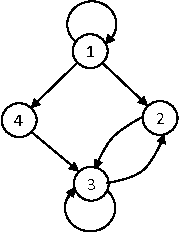
\includegraphics[scale=0.9]{Graficos/fig1_RB}		}{  \caption*{Grafo \(R\)}	}
	%
\end{floatrow}
\end{figure}
%


\subparagraph{Relaciones derivadas.}

Sea \(R\) una relación sobre el conjunto \(X\), la relación inversa \(R^{-1}\), el complemento \(R^{c}\) de la relación \(R\) se definen por:
\begin{align*}
    R^{-1} &= \big\{(x,y) \in X : \,(y,x) \in R \big\} \\
    R^{c} &= \big\{(x,y) \in X : \, (y,x) \not \in R\big\} 
\end{align*}

\subparagraph{Relación identidad.}

Relaciones identidad es:
\[
	I_d = \big\{ (x,x) : \, x \in X \big\}
\]


\subparagraph{Composición de relaciones.}

Si \(R\) y \(T\) son dos relaciones sobre \(X\), la relación compuesta \(RT\) se define por: \(x \, RT \, y\) ssi para algún \(z \in X, \; x \, R\, z \wedge z \, T\, y\).

%
\vspace{1\baselineskip}
\textbf{EJEMPLO 2:}

Sean \(R\) y \(T\) las relaciones definidas por las siguientes matrices:

%
\begin{table}[H]
	\fontsize{7}{11}\selectfont
    %\caption{Global caption}
    \begin{minipage}{.5\linewidth}
      %\caption{}
      \centering
	\begin{tabular}{c|ccccc} \thickline
	\(R\) & \(A_1\) & \(A_2\) & \(A_3\) & \(A_4\) & \(A_5\)  \\	\hline
    \(A_1\) & 1 & 1 & 0 & 1 & 1  \\
    \(A_2\) & 0 & 1 & 1 & 0 & 1  \\
	\(A_3\) & 0 & 1 & 0 & 1 & 0   \\
	\(A_4\) & 1 & 0 & 1 & 0 & 1   \\
	\(A_5\) & 0 & 0 & 1 & 0 & 1   \\
\end{tabular}
\label{tab:B2} 
    \end{minipage}%
    \begin{minipage}{.5\linewidth}
      \centering
        %\caption{}
	\begin{tabular}{c|ccccc} \thickline
	\(T\) & \(A_1\) & \(A_2\) & \(A_3\) & \(A_4\) & \(A_5\)  \\	\hline
    \(A_1\) & 0 & 1 & 0 & 1 & 0  \\
    \(A_2\) & 0 & 0 & 1 & 0 & 0  \\
	\(A_3\) & 1 & 0 & 0 & 1 & 0   \\
	\(A_4\) & 0 & 0 & 0 & 1 & 1   \\
	\(A_5\) & 1 & 1 & 0 & 0 & 1   \\
\end{tabular}
\label{tab:B3}
    \end{minipage} 
\end{table}
%

\vfill
\newpage

Entonces

\begin{table}[H]
   \fontsize{7}{11}\selectfont
    \begin{minipage}{.5\linewidth}
      \centering
	\begin{tabular}{c|ccccc} \thickline
	\(R^{-1}\) & \(A_1\) & \(A_2\) & \(A_3\) & \(A_4\) & \(A_5\)  \\
	\hline
    \(A_1\) & 1 & 0 & 0 & 1 & 0  \\
    \(A_2\) & 1 & 1 & 1 & 0 & 0  \\
	\(A_3\) & 0 & 1 & 0 & 1 & 1   \\
	\(A_4\) & 1 & 0 & 1 & 0 & 0   \\
	\(A_5\) & 1 & 1 & 0 & 1 & 1   \\
\end{tabular}
\label{tab:B4} 
    \end{minipage}%
    \begin{minipage}{.5\linewidth}
      \centering
        %\caption{}
	\begin{tabular}{c|ccccc} \thickline
	\(R^{c}\) & \(A_1\) & \(A_2\) & \(A_3\) & \(A_4\) & \(A_5\)  \\
	\hline
    \(A_1\) & 0 & 0 & 1 & 0 & 0  \\
    \(A_2\) & 1 & 0 & 0 & 1 & 0  \\
	\(A_3\) & 1 & 0 & 1 & 0 & 1   \\
	\(A_4\) & 0 & 1 & 0 & 1 & 0   \\
	\(A_5\) & 1 & 1 & 0 & 1 & 0   \\
\end{tabular}
\label{tab:B5} 
    \end{minipage} 
\end{table}

\begin{table}[H]
\fontsize{7}{11}\selectfont
\begin{center}
	\begin{tabular}{c|ccccc} \thickline
	\(RT\) & \(A_1\) & \(A_2\) & \(A_3\) & \(A_4\) & \(A_5\)  \\
	\hline
    \(A_1\) & 1 & 1 & 1 & 1 & 1  \\
    \(A_2\) & 1 & 0 & 0 & 1 & 0  \\
	\(A_3\) & 0 & 0 & 1 & 1 & 1   \\
	\(A_4\) & 1 & 1 & 0 & 1 & 0   \\
	\(A_5\) & 1 & 1 & 0 & 1 & 1   \\
\end{tabular}
\label{tab:B6} 
\end{center}
\end{table}

\textbf{Observación:} La matriz asociada a \(RT\) es el producto booleano \footnote{La suma y el producto booleano se definen por: \(0+0 = 0\), \( 0+1 = 1+0 = 1\), \(1+1 = 1\); \( 0\times0 = 0\), \( 0\times1 = 1\times0 = 0\), \( 1\times 1 = 1\).} de las matrices \(R\) y \(T\).\\

Para simplificar la escritura escribimos <<ssi>> en lugar de <<si y solo si>>.

\subparagraph{Propiedades de las relaciones.}

Se dice que la relación \(R\) satisface la propiedad:

\begin{table}[H]
\fontsize{7.5}{11}\selectfont
\begin{center}
\begin{tabular}{l l l l l}
	Reflexiva & ssi & \(x \, R \, x\) & ssi & \(I_d \subset R\)  \\
    Irreflexiva & ssi & \( \neg(x \, R \, x)\) & ssi & \(R \subset I_d^{c}\)  \\
    Simétrica & ssi & \( (x \, R \, y) \Longrightarrow (y \, R \, x)\) & ssi & \(R = R^{-1}\)  \\
    Asimétrica & ssi & \( (x \, R \, y) \Longrightarrow \neg (y \, R \, x)\) & ssi & \(R \cap R^{-1} = \varnothing \)  \\
    Antisimétrica & ssi & \( (x \, R \, y) \wedge (y \, R \, x) \Longrightarrow (x = y)\) & ssi & \(R \cap R^{-1} = I_d\)  \\
    Transitiva & ssi & \( (x \, R \, y) \wedge (y \, R \, z) \Longrightarrow (x \, R \, z)\) & ssi & \(RR \subset R\)  \\
    Semitransitiva & ssi & \( (x \, R \, y) \wedge (y \, R \, z) \Longrightarrow (x \, R \, u) \vee (u \, R \, z) \) & ssi & \(PPI \subset P\) \; \text{ssi} \; \(IPP \subset P\) \\
    Ferrers & ssi & \( (x \, R \, y) \wedge (z \, R \, u) \Longrightarrow (x \, R \, u) \vee (z \, R \, y) \) & ssi & \(PIP \subset P\)\\
    Completa & ssi & \( (x \, R \, y) \vee (y \, R \, x) \) & ssi & \(X^2 = R \cup R^{-1}\)  \\
    Cuasi completa & ssi & \( x \neq y \Longrightarrow (x \, R \, y) \vee (y \, R \, x) \) & ssi & \(X^2 \backslash I_d = R \cup R^{-1}\)  \\[-2\baselineskip]
\end{tabular}
\label{tab:B7} 
\end{center}
\end{table}



Para todo \(x,y,z,u \in X\), según corresponda.

La completitud y cuasi completitud se denominan también completitud fuerte y completitud
respectivamente \citeA{Ozturke-2003}.

\newpage

\subparagraph{Relaciones de orden.}

Sean \(I\), \(P\) y \(R\) relaciones definidas sobre el conjunto \(X\). Se dice que \(R\) es una relación de:

\begin{table}[H]
\fontsize{8}{11}\selectfont
\begin{center}
\begin{tabular}{l l l }
	Orden parcial      & ssi & \(R\) es reflexiva, antisimétrica y transitiva  \\
	                   & ssi & \(I_d \subset R\), \( R \cap R^{-1} \subset I_d \) y \(RR \subset R \)\\
    Pre-orden parcial  & ssi & \(R\) es reflexiva y transitiva \\
                       & ssi & \(I_d \subset R\) y \(RR \subset R \)\\
    Semi-orden parcial & ssi & \(R\) es reflexiva, Ferrers y semitransitiva \\
                       & ssi & \(I_d \subset R\), \(PIP \subset P\) y \(PPI \subset P \)\\[-1\baselineskip]
\end{tabular}
\label{tab:B8} 
\end{center}
\end{table}

\vspace{-1\baselineskip}

Una relación de orden, preorden o semiorden parcial es una relación de orden, preorden o semiorden total ssi la relación es completa ssi \(X^2 = R \cup R^{-1}\).

La relación \(P\) se denomina:

\begin{table}[H]
\fontsize{7.5}{11}\selectfont
\begin{center}
	\begin{tabular}{l l l }
		Orden estricto parcial & si & \(P\) es asimétrica y transitiva \\
	    	                   & ssi & \(P \cap P^{-1} = \varnothing \) y \(PP \subset P \)\\[-1\baselineskip]
	\end{tabular}
	\label{tab:B9} 
\end{center}
\end{table}

\vspace{-1\baselineskip}

Una relación de orden estricta parcial es una relación de orden estricta total ssi la relación es cuasi-completa ssi \(X^2  \backslash  I_d = R \cup R^{-1}\).

El par \((X,R)\) o \((X,P)\) se denomina estructura de orden.

La relación \(I\) se denomina de:

\begin{table}[H]
\fontsize{7.5}{11}\selectfont
\begin{center}
	\begin{tabular}{l l l }
		Semejanza & si & \(I\) es reflexiva y simétrica \\
	    	      & ssi & \(I_d \subset I \), \(I = I^{-1} \)\\
		Equivalencia & si & \(I\) es reflexiva, simétrica y transitiva \\
	          	     & ssi & \(I_d \subset I \), \(I = I^{-1} \) y \(II \subset I\)\\[-1\baselineskip]
	\end{tabular}
\label{tab:B10} 
\end{center}
\end{table}

\vspace{-1\baselineskip}

La clase de equivalencia de \(x \in X\) para la relación de equivalencia \(I\), se define por:
\[
	[x] = \big\{y \in X : x \, I \, y \big\}
\]

\textbf{Observación:}

\begin{APAenumerate}
    \item La completitud implica la reflexividad; la asimetría la irreflexividad; y, la completitud implica la cuasi-completitud.
    \item La completitud es un supuesto de partida en la economía convencional (mainstream). La economía ecológica por el contrario considera la comparabilidad débil de valores como uno de sus fundamentos (Alier et al 1998). Siendo este el caso, queda abierta completamente la posibilidad de no comparabilidad entre alternativas, lo que lleva a estructuras de orden parcial.
\end{APAenumerate}


\vfill
\newpage

Ejemplos de las distintas estructuras de orden.


\vspace{1\baselineskip}
\textbf{EJEMPLO 3:} Orden total

\begin{table}[H]
\begin{floatrow}
	\fontsize{7}{11}\selectfont
	\captionsetup{justification=centering, labelfont=footnotesize, font=footnotesize}
	%	Tabla
	\capbtabbox{%
	 \begin{tabular}{c|cccc} \thickline
	\(R\) & \(A_1\) & \(A_2\) & \(A_3\) & \(A_4\)   \\ \hline
    \(A_1\) & 1 & 0 & 0 & 1  \\
    \(A_2\) & 1 & 1 & 1 & 1  \\
	\(A_3\) & 1 & 0 & 1 & 1  \\
	\(A_4\) & 0 & 0 & 0 & 1  \\
	\end{tabular}
	\vspace{0.35cm}
	}{	  %\caption*{Matriz \(R\) \\ El nodo \(A_i\) se etiqueta únicamente \(i\).}%
	}
	\capbtabbox{%
	 \begin{tabular}{c|cccc} \thickline
	\(R\) & \(A_2\) & \(A_3\) & \(A_1\) & \(A_4\)   \\ \hline
    \(A_2\) & 1 & 1 & 1 & 1  \\
    \(A_3\) & 0 & 1 & 1 & 1  \\
	\(A_1\) & 0 & 0 & 1 & 1  \\
	\(A_4\) & 0 & 0 & 0 & 1  \\
	\end{tabular}
	}{	  \caption*{(reordenando \(X\))}%
	}
\end{floatrow}
\end{table}

\[
	R: A_2 > A_3 > A_1 > A_4
\]

\begin{figure}[H]
    \centering
    
\includegraphics[scale=0.9]{Graficos/fig2_RB}
    \label{fig:RB_grafo2}
\end{figure}

En un orden total finito los elementos pueden ordenarse uno detrás de otro, por ello se lo denomina también orden lineal. La relación \(P = R \backslash I\) es un orden estricto.

Para visibilizar de mejor manera, en un grafo no se grafican los arcos que se pueden obtenerse por la aplicación de la transitividad. Así en un orden lineal se suele graficar únicamente los arcos que enlazan un nodo al siguiente.

El ejemplo paradigmático de orden total es el orden usual <<mayor o igual>> (\(\geq\)) en los números naturales o en los números reales.

\vspace{1\baselineskip}
\textbf{EJEMPLO 4:} Preorden 

\begin{table}[H]
\begin{floatrow}
	\fontsize{7}{11}\selectfont
	\captionsetup{justification=centering, labelfont=footnotesize, font=footnotesize}
	%	Tabla
	\capbtabbox{%
	 \begin{tabular}{c|ccccc} \thickline
	\(R\) & \(A_1\) & \(A_2\) & \(A_3\) & \(A_4\) & \(A_5\)    \\ \hline
    \(A_1\) & 1 & 0 & 0 & 1 & 0  \\
    \(A_2\) & 1 & 1 & 0 & 1 & 0  \\
	\(A_3\) & 1 & 1 & 1 & 1 & 1  \\
	\(A_4\) & 1 & 0 & 0 & 1 & 0  \\
	\(A_5\) & 1 & 1 & 1 & 1 & 1  \\
	\end{tabular}
	\vspace{0.35cm}
	}{	  %\caption*{Matriz \(R\) \\ El nodo \(A_i\) se etiqueta únicamente \(i\).}%
	}
	\capbtabbox{%
	 \begin{tabular}{c|ccccc} \thickline
	\(R\) & \(A_3\) & \(A_5\) & \(A_2\) & \(A_1\) & \(A_4\)    \\ 	\hline
    \(A_3\) & 1 & 1 & 1 & 1 & 1  \\
    \(A_5\) & 1 & 1 & 1 & 1 & 1  \\
	\(A_2\) & 0 & 0 & 1 & 1 & 1   \\
	\(A_1\) & 0 & 0 & 0 & 1 & 1  \\
	\(A_4\) & 0 & 0 & 0 & 1 & 1  \\
	\end{tabular}
	}{	  \caption*{(reordenando \(X\))}%
	}
\end{floatrow}
\end{table}

\[
	R: A_3 = A_5 > A_2 > A_1 = A_4
\]

\begin{figure}[H]
    \centering
    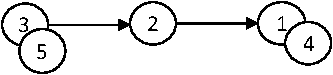
\includegraphics[scale=0.9]{Graficos/fig3_RB}
    \label{fig:RB_grafo2}
\end{figure}

Reordenando los elementos de \(X\) de ser necesario, la matriz de una relación de preorden es una matriz con 1’s en la triangular superior y una estructura de bloques cuadrados de 1’s disjuntos sobre la diagonal principal. Los bloques cuadrados determinan a las clases de equivalencia, pues \(I\) es una relación de equivalencia. En el ejemplo: \([A_3] = \{A_3, A_5\}\), \([A_2] = \{A_2\}\), \([A_1] = \{A_1, A_4\}\) y están totalmente ordenadas por la relación inducida \([x] \, R \, [y]\) si \( x \, R \, y\). En el ejemplo, \([A_3] \, R \, [A_2] \,  R \, [A_1]\). Las clases de equivalencia forman una partición de \(X\) (las clases de equivalencia son disjuntas y su unión es igual a \(X\)).

\vspace{1\baselineskip}
En la microeconomía se asume que las preferencias de los consumidores son un preorden sobre el conjunto de canastas de consumo; las <<curvas de indiferencia>> son las clases de equivalencia.

\vspace{1\baselineskip}
\textbf{EJEMPLO 5:} Semiorden 

\begin{table}[H]
\begin{floatrow}
	\fontsize{7}{11}\selectfont
	\captionsetup{justification=centering, labelfont=footnotesize, font=footnotesize}
	%	Tabla
	\capbtabbox{%
	 \begin{tabular}{c|ccccc} \thickline
	\(R\) & \(A_1\) & \(A_2\) & \(A_3\) & \(A_4\) & \(A_5\)    \\ \hline
    \(A_1\) & 1 & 0 & 1 & 1 & 1  \\
    \(A_2\) & 1 & 1 & 1 & 1 & 1  \\
	\(A_3\) & 1 & 0 & 1 & 0 & 0  \\
	\(A_4\) & 1 & 1 & 1 & 1 & 1  \\
	\(A_5\) & 1 & 1 & 1 & 1 & 1  \\
	\end{tabular}
	\vspace{0.9\baselineskip}
	}{	  %\caption*{Matriz \(R\) \\ El nodo \(A_i\) se etiqueta únicamente \(i\).}%
	}
	\capbtabbox{%
	 \begin{tabular}{c|ccccc} \thickline
	\(R\) & \(A_2\) & \(A_4\) & \(A_5\) & \(A_1\) & \(A_3\)    \\ 	\hline
    \(A_2\) & 1 & 1 & 1 & 1 & 1  \\
    \(A_4\) & 1 & 1 & 1 & 1 & 1  \\
	\(A_5\) & 1 & 1 & 1 & 1 & 1  \\
	\(A_1\) & 0 & 1 & 1 & 1 & 1  \\
	\(A_3\) & 0 & 0 & 0 & 1 & 1  \\
	\end{tabular}
	}{	  \caption*{(reordenando \(X\))}%
	}
\end{floatrow}
\end{table}

\vspace{-1\baselineskip}
\begin{figure}[H]
    \centering
    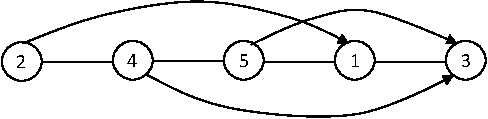
\includegraphics[scale=0.9]{Graficos/fig4_RB}
    \label{fig:RB_grafo4}
\end{figure}

En un semiorden, al reordenar los elementos de \(X\) de ser necesario, la matriz asociada tiene 1’s en la triangular superior y una estructura de bloques cuadrados de 1’s no necesariamente disjuntos sobre la diagonal principal. La matriz asociada es en <<escalera>>: la frontera entre los 0’s y 1’s tiene la forma de una escalera con los 0’s en la triangular inferior de la matriz \cite{Monjardet-1978}.

La relación \(I\) es una relación de semejanza. No es una relación transitiva.

En el grafo de un semiorden, los nodos se pueden graficar en secuencia, uno a continuación de otro (o uno debajo de otro), siguiendo el orden de los elementos en la matriz en escalera. Cada nodo se enlaza con el primer nodo estrictamente menor mediante un arco dirigido (flecha). El nodo <<padre>> será mayor al nodo hijo y a todos los nodos a la derecha (o inferiores). Esto permite graficar un conjunto limitado de arcos y visibilizar de mejor manera el grafo.

En el ejemplo, los bloques son: \(B_1 = \{A_2, A_4, A_5\}\), \(B_2 = \{A_4, A_5, A_1\}\), \(B_3 = \{A_1, A_3\}\). No son clases de equivalencia pues no son bloques disjuntos, pero son bloques consecutivos.

Nótese que en un semiorden los mejores elementos de \(X\) son los elementos de \(B_1 \backslash \cup _{i \geq 2} B_i\). Los elementos de este conjunto son máximos, satisfacen que para todo \(y \in X\), \(x \, R \, y\).

\vspace{1\baselineskip}
Un semiorden es una estructura adecuada para modelar y evitar la <<paradoja de Luce>> en la microeconomía tradicional: Un consumidor prefiere estrictamente una taza de café con dos cucharadas de azúcar (\(10 [gr]\)) a una taza de café sin azúcar. Por otra parte, el consumidor es indiferente entre dos tazas de café con \(z\) y \(z + \epsilon\) gramos de azúcar (\(0 \geq z \geq 10\); \(\epsilon = 0.01\)). Si se forma la cadena indiferencia de tazas de café con: \(0\); \(0,01\); \(0,02\); \(\dots\); \(9,98\); \(9,99\); \(10\) gramos de azúcar; al final se concluirá que el consumidor es indiferente entre la taza de café con \(10 [gr]\) de azúcar y la taza de café sin azúcar.

\vspace{1\baselineskip}
\textbf{EJEMPLO 6:} Orden parcial

\begin{figure}[H]
\begin{floatrow}
	\fontsize{7}{11}\selectfont
	\captionsetup{justification=centering, labelfont=footnotesize, font=footnotesize}
	%	Tabla
	\capbtabbox{%
	 \begin{tabular}{c|cccc} \thickline
	\(R\) & \(A_2\) & \(A_3\) & \(A_1\) & \(A_4\) \\ \hline
    \(A_2\) & 1 & 1 & 1 & 0   \\
    \(A_3\) & 0 & 1 & 0 & 1   \\
	\(A_1\) & 0 & 0 & 1 & 1   \\
	\(A_4\) & 0 & 0 & 0 & 1   \\
	\end{tabular}
	\vspace{2em}
	}{	  \caption*{}%
	}
	%	Figura
	\ffigbox{	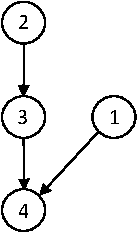
\includegraphics[scale=0.75]{Graficos/fig5_RB}		}{  \caption*{}	}
	%
\end{floatrow}
\end{figure}

\vspace{-2\baselineskip}
La estructura de orden parcial es bastante común. Por ejemplo, los elementos de una familia de subconjuntos de un conjunto están relacionados por un orden parcial

\vspace{1\baselineskip}
\textbf{EJEMPLO 7:} Preorden parcial

\vspace{1\baselineskip}
\begin{figure}[H]
\begin{floatrow}
	\fontsize{7}{11}\selectfont
	\captionsetup{justification=centering, labelfont=footnotesize, font=footnotesize}
	%	Tabla
	\capbtabbox{%
	 \begin{tabular}{c|ccccc} \thickline
	\(R\) & \(A_3\) & \(A_5\) & \(A_2\) & \(A_1\) & \(A_4\)     \\ \hline
    \(A_3\) & 1 & 1 & 1 & 1 & 1  \\
    \(A_5\) & 1 & 1 & 1 & 1 & 1  \\
	\(A_2\) & 0 & 0 & 1 & 0 & 0  \\
	\(A_1\) & 0 & 0 & 0 & 1 & 1  \\
	\(A_4\) & 0 & 0 & 0 & 1 & 1  \\
	\end{tabular}
	}{	  \caption*{}%
	}
	%	Figura
	%\vspace{-1\baselineskip}
	\ffigbox{	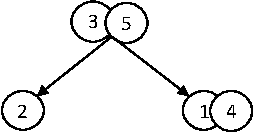
\includegraphics[scale=0.75]{Graficos/fig6_RB}		}{  \caption*{}	}
	%
\end{floatrow}
\end{figure}

\vspace{-1\baselineskip}
\textbf{EJEMPLO 8:} Semiorden parcial

\vspace{-2.3\baselineskip}
\begin{figure}[H]
\begin{floatrow}
	\fontsize{7}{11}\selectfont
	\captionsetup{justification=centering, labelfont=footnotesize, font=footnotesize}
	%	Tabla
	\capbtabbox{%
	 \begin{tabular}{c|ccccc} \thickline
	\(R\) & \(A_2\) & \(A_4\) & \(A_5\) & \(A_1\) & \(A_3\)    \\ 	\hline
    \(A_2\) & 1 & 0 & 1 & 1 & 1  \\
    \(A_4\) & 0 & 1 & 1 & 1 & 1  \\
	\(A_5\) & 0 & 1 & 1 & 1 & 1  \\
	\(A_1\) & 0 & 0 & 1 & 1 & 1  \\
	\(A_3\) & 0 & 0 & 0 & 1 & 1  \\
	\end{tabular}
	\vspace{2em}
	}{	  \caption*{}%
	}
	%	Figura
	\ffigbox{	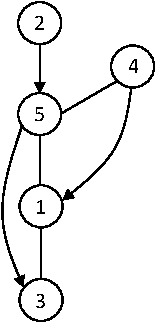
\includegraphics[scale=0.75]{Graficos/fig7_RB}		}{  \caption*{}	}
	%
\end{floatrow}
\end{figure}

\vfill
\newpage

\paragraph{Estructura \(I-P-J\).}

La tripleta \(I\), \(P\), \(J\) de relaciones sobre \(X\) se denomina una estructura de preferencia \(I-P-J\) ssi satisface las condiciones:

\vspace{1\baselineskip}
\begin{APAenumerate}
    \item \(I\) es reflexiva y simétrica.
    \item \(P\) es asimétrica.
    \item \(J\) es irreflexiva y simétrica.
    \item \(P \cap I = P \cap J = I \cap J = \varnothing\).
    \item \(X^2 = I \cup P \cup P^{-1} \cup J\). 
    \item La relación característica o relación grande \(R\) se define por \(R = I \cup P\)
\end{APAenumerate}

\vspace{1\baselineskip}
Si \(J = \varnothing\), la estructura de preferencia se denomina estructura \(I-P\).


\vspace{1\baselineskip}
\textbf{EJEMPLO 9:} 
Para la relación \(R\) del ejemplo 2. Se tiene que:

\begin{table}[H]
	\fontsize{7}{11}\selectfont
    %\caption{Global caption}
    \begin{minipage}{.5\linewidth}
      %\caption{}
      \centering
	\begin{tabular}{c|ccccc} \thickline
	\(R\) & \(A_1\) & \(A_2\) & \(A_3\) & \(A_4\) & \(A_5\)  \\ \hline
    \(A_1\) & 1 & 1 & 0 & 1 & 1  \\
    \(A_2\) & 0 & 1 & 0 & 0 & 1  \\
	\(A_3\) & 0 & 1 & 1 & 1 & 0   \\
	\(A_4\) & 1 & 0 & 1 & 1 & 1   \\
	\(A_5\) & 0 & 0 & 1 & 0 & 1   \\
\end{tabular}
\label{tab:B2} 
    \end{minipage}%
    \begin{minipage}{.5\linewidth}
      \centering
        %\caption{}
	\begin{tabular}{c|ccccc} \thickline
	\(R^{-1}\) & \(A_1\) & \(A_2\) & \(A_3\) & \(A_4\) & \(A_5\)  \\ \hline
    \(A_1\) & 1 & 1 & 0 & 1 & 1  \\
    \(A_2\) & 0 & 1 & 1 & 0 & 1  \\
	\(A_3\) & 0 & 0 & 1 & 1 & 0   \\
	\(A_4\) & 1 & 0 & 1 & 1 & 1   \\
	\(A_5\) & 0 & 0 & 1 & 0 & 1   \\
\end{tabular}
\label{tab:B3}
    \end{minipage} 
\end{table}
%

\begin{table}[H]
   \fontsize{7}{11}\selectfont
    \begin{minipage}{.5\linewidth}
      \centering
	\begin{tabular}{c|ccccc} \thickline
	\(I\) & \(A_1\) & \(A_2\) & \(A_3\) & \(A_4\) & \(A_5\)  \\ \hline
    \(A_1\) & 1 & 0 & 0 & 1 & 0  \\
    \(A_2\) & 0 & 1 & 0 & 0 & 0  \\
	\(A_3\) & 0 & 1 & 1 & 1 & 0   \\
	\(A_4\) & 1 & 0 & 1 & 1 & 0   \\
	\(A_5\) & 0 & 0 & 0 & 0 & 1   \\
\end{tabular}
\label{tab:B4} 
    \end{minipage}%
    \begin{minipage}{.5\linewidth}
      \centering
        %\caption{}
	\begin{tabular}{c|ccccc} \thickline
	\(P\) & \(A_1\) & \(A_2\) & \(A_3\) & \(A_4\) & \(A_5\)  \\ \hline
    \(A_1\) & 0 & 1 & 0 & 0 & 1  \\
    \(A_2\) & 0 & 0 & 0 & 0 & 1  \\
	\(A_3\) & 0 & 1 & 0 & 0 & 0   \\
	\(A_4\) & 0 & 0 & 0 & 0 & 1   \\
	\(A_5\) & 0 & 0 & 1 & 0 & 0   \\
\end{tabular}
\label{tab:B5} 
    \end{minipage} 
\end{table}

%

\begin{table}[H]
   \fontsize{7}{11}\selectfont
    \begin{minipage}{.5\linewidth}
      \centering
	\begin{tabular}{c|ccccc} \thickline
	\(P^{-1}\) & \(A_1\) & \(A_2\) & \(A_3\) & \(A_4\) & \(A_5\)  \\ \hline
    \(A_1\) & 0 & 0 & 0 & 0 & 0  \\
    \(A_2\) & 1 & 0 & 1 & 0 & 0  \\
	\(A_3\) & 0 & 0 & 0 & 0 & 1   \\
	\(A_4\) & 0 & 0 & 0 & 0 & 0   \\
	\(A_5\) & 1 & 1 & 0 & 1 & 0   \\
\end{tabular}
\label{tab:B4} 
    \end{minipage}%
    \begin{minipage}{.5\linewidth}
      \centering
        %\caption{}
	\begin{tabular}{c|ccccc} \thickline
	\(J\) & \(A_1\) & \(A_2\) & \(A_3\) & \(A_4\) & \(A_5\)  \\ \hline
    \(A_1\) & 0 & 0 & 1 & 0 & 0  \\
    \(A_2\) & 0 & 0 & 0 & 1 & 0  \\
	\(A_3\) & 1 & 0 & 0 & 0 & 0   \\
	\(A_4\) & 0 & 1 & 0 & 0 & 0   \\
	\(A_5\) & 0 & 0 & 0 & 0 & 0   \\
\end{tabular}
\label{tab:B5} 
    \end{minipage} 
\end{table}

\paragraph{Matriz de relaciones o matriz coloreada.}

La información anterior puede resumirse en la matriz de relaciones definida por:
\begin{align*}
    R_0 : X \times X & \longrightarrow \big\{I, P , P^{-1}, J \big\} \\
    (x,y) & \mapsto R_0(x,y) = \text{argmax} \big\{R_k(x,y)\big\}
\end{align*}

Es decir, a cada par \((x,y)\) se le asocia el símbolo de la relación que se satisface en el par. Para destacar las relaciones se pinta o colorea el fondo de la celda con: amarillo para la indiferencia, celeste para la preferencia estricta, verde para la preferencia estricta inversa, y gris para la indiferencia.


\vspace{1\baselineskip}
\textbf{EJEMPLO 10:} Continuando con el ejemplo 9.

\begin{table}[H]
   \fontsize{7}{11}\selectfont
   	\captionsetup{justification=centering, labelfont=footnotesize, font=footnotesize}
    \centering
	\begin{tabular}{c|ccccc} \thickline
	\(R_0\) & \(A_1\) & \(A_2\) & \(A_3\) & \(A_4\) & \(A_5\)  \\ \hline
    \(A_1\) & \cellcolor{pastelyellow} I & \cellcolor{paleblue} P & \cellcolor{pastelgray}J & \cellcolor{pastelyellow} I & \cellcolor{paleblue} P  \\
    \(A_2\) &  & \cellcolor{pastelyellow} I & \cellcolor{palegreen} \(P^{-1}\) & \cellcolor{pastelgray}J & \cellcolor{paleblue} P  \\
	\(A_3\) &  &  & \cellcolor{pastelyellow} I & \cellcolor{pastelyellow} I & \cellcolor{palegreen} \(P^{-1} \)  \\
	\(A_4\) &  &  &  & \cellcolor{pastelyellow} I & \cellcolor{paleblue} P   \\
	\(A_5\) &  &  &  &  & \cellcolor{pastelyellow}I   \\
    \end{tabular}
    \caption*{Matriz coloreada}
\label{tab:B4} 
\end{table}

	\subsubsection{Conjuntos difusos.}

En un conjunto <<clásico>>, no difuso, dado un conjunto \(A\) y un elemento \(x\), se tiene que: \(x\) pertenece a \(A\) o, \(x\) no pertenece a \(A\). Por ejemplo si \(A = \{x : x \, \text{es alto}\}\) y \(x = \text{Jorge}\), se tiene que Jorge es alto o Jorge no es alto. Si, digamos, Jorge mide \(1.90 [m]\) (y lo consideramos alto), ¿qué se puede decir de Santiago que mide \(1.85 [m]\) y de María que mide \(1.60[m]\)?

Posiblemente la respuesta sea: Santiago es medianamente alto, María es muy poco alta. Los conjuntos difusos permiten expresar estas ideas. En los conjuntos clásicos se puede definir una función de pertenencia al conjunto \(A\) que toma el valor 1 si \(x \in A\) y vale 0 si \(x \not \in A\) (y solo toma estos valores). En los conjuntos difusos, la función grado de pertenencia al conjunto difuso \(A\) puede ser cualquier valor entre 0 y 1. El grado de pertenencia igual a 0 significará que es absoluta y totalmente certero que \(x \not \in A\). El grado de pertenencia igual a 1 significará que es absoluta y totalmente certero que \(x \in A\). Así, para el conjunto difuso \(A\) (el conjunto de los altos), se tendrá que \(\text{gr}(\text{Jorge} \in A) = 1\); \(\text{gr}(\text{Santiago} \in A) = 0.90\); \(\text{gr}(\text{María} \in A) = 0.30\). Veamos ahora la definición formal de conjunto difuso. 

\paragraph{Conjuntos difusos.}

Sea \(X\) un conjunto cualesquiera que lo denominaremos universo del discurso.

\begin{APAitemize}
    \item Un conjunto difuso \(A\) es una función \(\mu _A: X \rightarrow [0,1]\) que para cada elemento de \(x \in X\) asocia el grado de pertenencia, o la credibilidad de la pertenencia, de \(x\) al conjunto \(A\). Se nota \(\mu _A(x) = \text{gr}(x \in A)\).
    
    \item Una relación difusa \(R\) sobre \(X\) es un subconjunto difuso en \(X \times X\). El grado de pertenencia del par \((x,y) \in X \times X\) al conjunto \(R\) se nota \(R(x,y)\). Se dice también que \(R(x,y)\) el grado de credibilidad, o simplemente credibilidad, de la relación \(R(x,y)\).
\end{APAitemize}

\paragraph{Operaciones entre conjuntos difusos.}

Las operaciones clásicas entre conjuntos: unión, intersección y complemento se extienden a los conjuntos difusos de la siguiente manera:

\subparagraph{Complemento.}

Un complemento difuso de un conjunto difuso \(A\) es una función \(N\) que al grado de pertenencia al conjunto difuso \(A\) le asocia el grado de pertenencia al conjunto difuso complemento \(A^{c}\).
    \begin{align*}
    N: [0,1] & \longrightarrow [0,1]\\
    \mu _A(x) & \longrightarrow N(\mu _A(x)) = \mu _{A^{c}}(x)
    \end{align*}

Cumple las condiciones siguientes:
\begin{align*}
	\text{condiciones de borde:	}&	& N(0) &= 1,\qquad  N(1) = 0,
	\\
	\text{monotonía creciente:		}&	& a&<b	\Rightarrow N(a) \geq N(b).
\end{align*}

Adicionalmente se puede exigir el cumplimiento de las condiciones siguientes:
\begin{APAitemize}
    \item \(N\) es una función continua.
    \item \(N\) es estrictamente decreciente, en tal caso se denomina negación estricta.
    \item \(N\big(N(a)\big) = a\), involución. De ser este el caso se denomina negación fuerte.
\end{APAitemize}

\subparagraph{Intersección.}
La intersección difusa de dos conjuntos difusos \(A\) y \(B\) es una función \(T\), denominada norma triangular o t-norma, que al par de grados de pertenencia de un elemento a los conjuntos \(A\) y \(B\) le asocia el grado de pertenencia al conjunto difuso intersección \(A \cap _T B\).
    \begin{align*}
    T: [0,1] \times [0,1] & \longrightarrow [0,1]\\
    (\mu _A(x), \mu _B(x)) & \longrightarrow T(\mu _A(x), \mu _B(x)) = \mu_{A\cap B} (x)
    \end{align*}

Cumple las condiciones:
\begin{align*}
	T(1,a) &= a 		&	\text{condiciones de borde}	\\
	T(a,b) &= T(b,a) 	&	\text{conmutatividad}			\\
	a \leq a' \wedge b \leq b' &\Rightarrow T(a,b) \leq T(a',b')	&	\text{monotonía no decreciente}			\\
	T\big(T(a,b),c\big) &= T\big(a, T(b,c)\big)	&		\text{asociatividad}			\\
\end{align*}

    
Adicionalmente se puede exigir el cumplimiento de la condición:

\begin{center}
	\(T\) es una función continua.
\end{center}

\subparagraph{Unión.}

La unión difusa de dos conjuntos difusos \(A\) y \(B\) es una función \(S\), denomina co-norma triangular o t-conorma o s-norma, que al par de grados de pertenencia a \(A\) y \(B\) le asocia el grado de pertenencia al conjunto difuso unión  \(A \cup _S B\).
    \begin{align*}
    S: [0,1] \times [0,1] & \longrightarrow [0,1]\\
    (\mu _A(x), \mu _B(x)) & \longrightarrow S(\mu _A(x), \mu _B(x)) = \mu_{A\cup B} (x)
    \end{align*}

Cumple las condiciones:
\begin{align*}
	S(0,a) &= a 		&	\text{condiciones de borde}	\\
	S(a,b) &= S(b,a) 	&	\text{conmutatividad}			\\
	a \leq a' \wedge b \leq b' &\Rightarrow S(a,b) \leq S(a',b')	&	\text{monotonía no decreciente}			\\
	S\big(S(a,b),c\big) &= S\big(a, S(b,c)\big)	&		\text{asociatividad}			\\
\end{align*}
 
Adicionalmente se puede exigir el cumplimiento de la condición:

\begin{center}
	\(S\) es una función continua.
\end{center}

\vspace{1\baselineskip}
\textbf{EJEMPLO 11:}

\begin{APAenumerate}
    \item La negación usual es la función \(N(a)=1-a\).
    \item La t-norma y la t-conorma de Frank de parámetro \(s\), son:
    \begin{align*}
    	T^s(a,b) & = \log _s \left(1+\dfrac{(s^a -1)(s^b-1)}{s-1}\right),			\\	
    	S^s(a,b) & = 1- \log _s \left(1+\dfrac{(s^{1-a} -1)(s^{1-b}-1)}{s-1}\right), 	\qquad s \in (0,\infty).
    \end{align*}

    \item La t-norma y la t-conorma de Lukasiewics son:
    \begin{align*}
    	T(a,b) & = \max (a+b-1,0),		\\
    	S(a,b) & = \min (a+b,1).
    \end{align*}    
    
\end{APAenumerate}

\textbf{Observación:} La negación usual, la t-norma y la t-conorma de Frank de parámetro \(s\); la negación usual, la t-norma y la t-conorma de Lukasiewics son tripletas de De Morgan; es decir, satisfacen las leyes de De Morgan:
\begin{align*}
	(A \cup_S B)^c &= A^c \cap_T B^c	,
	\\
	(A \cap_T B)^c &= A^c \cup_S B^c	.
\end{align*}

La t-norma y la t-conorma de Frank de parámetro \(s\), satisface que:
    \begin{align*}
    	\lim _{s \rightarrow 1} T^s(a,b) & = T^1(a,b)  = ab,	\\
    	\lim _{s \rightarrow \infty} S^s(a,b) & = S^{\infty} (a,b)  = \min (a+b,1).
    \end{align*}  

\paragraph{Estructura \(I-P-J\) difusa.}

En el modelo no difuso, a partir de la preferencia débil \(R\) las relaciones \(I\), \(P\), \(J\) se definen mediante una estructura \(I-P-J\). En el caso de que \(R\) es una preferencia difusa, la estructura \(I-P-J\) también será difusa. Para ello, en el marco conceptual definido por \citeA{Fodor-1994}, se aplica una versión simplificada el teorema de \citeA{Alcina-1985}.

\subparagraph{Teorema \cite{Alsina-1985}.}

Sean \((X,R)\) una estructura de preferencia difusa donde \(R\) es una preferencia débil difusa definida sobre \(X\), \(N\) un complemento difuso, \(T\) una t-norma, \(S\) una t-conorma. La estructura de preferencia difusa \(I-P-J\) definida por:

\[
	I = R \cap_T R^{-1}, \qquad P = R \cap_T R^{{-1}^c}, \qquad J = R^{c} \cap_T R^{{-1}^c}
\]

satisface las condiciones:
\[
	R = I \cup_S P, \qquad R^{{-1}^c} = P \cup_S J, \qquad X \times X = I \cup P \cup P^{-1} \cup J 
\]

Si y solo si

\begin{APAitemize}
    \item \(N\) es la negación usual \(\big(N(a) = 1-a\big)\)
    \item \(T\) es la t-norma de Frank de parámetro \(s = 1\), \(T^1(a,b) = ab\)
    \item \(S\) es la t-conorma de Frank de parámetro \(s = \infty\), \(S^{\infty}(a,b) = \min(a+b, 1)\)
\end{APAitemize}

\subparagraph{Corolario}

Al aplicar el teorema de Alsina se obtiene:
\[
	I = R*R^{-1}, \qquad P = R*(1-R^{-1}), \qquad P^{-1} = (1-R)*R^{-1}, \qquad J = (1-R)*(1-R^{-1})
\]

\vspace{1\baselineskip}
\textbf{EJEMPLO 12:} Consideremos la estructura difusa \(I-P-J\) determinada por la relación difusa reflexiva \(R\).

\begin{table}[H]
	\fontsize{7}{11}\selectfont
    %\caption{Global caption}
    \begin{minipage}{.5\linewidth}
      %\caption{}
      \centering
	\begin{tabular}{c|ccccc} \thickline
	\(R\) & \(A_1\) & \(A_2\) & \(A_3\) & \(A_4\) & \(A_5\)  \\ \hline
    \(A_1\) & 1 & 0.6 & 0.3 & 1 & 1  \\
    \(A_2\) & 0.8 & 1 & 0.4 & 0.9 & 1  \\
	\(A_3\) & 0.3 & 0.1 & 1 & 0.3 & 0.4   \\
	\(A_4\) & 0 & 0.1 & 0.8 & 1 & 0.9   \\
	\(A_5\) & 0.2 & 0.3 & 0.2 & 0.2 & 1   \\
\end{tabular}
\label{tab:B2} 
    \end{minipage}%
    \begin{minipage}{.5\linewidth}
      \centering
        %\caption{}
	\begin{tabular}{c|ccccc} \thickline
	\(R^{-1}\) & \(A_1\) & \(A_2\) & \(A_3\) & \(A_4\) & \(A_5\)  \\ \hline
    \(A_1\) & 1 & 0.6 & 0.3 & 1 & 1  \\
    \(A_2\) & 0.8 & 1 & 0.4 & 0.9 & 1  \\
	\(A_3\) & 0.3 & 0.1 & 0.8 & 1 & 0.9   \\
	\(A_4\) & 0 & 0.1 & 0.8 & 1 & 0.9   \\
	\(A_5\) & 0.2 & 0.3 & 0.2 & 0.2 & 1   \\
\end{tabular}
\label{tab:B3}
    \end{minipage} 
\end{table}
%

\begin{table}[H]
   \fontsize{7}{11}\selectfont
    \begin{minipage}{.5\linewidth}
      \centering
	\begin{tabular}{c|ccccc} \thickline
	\(I\) & \(A_1\) & \(A_2\) & \(A_3\) & \(A_4\) & \(A_5\)  \\ \hline
    \(A_1\) & 1 & 0.48 & 0.09 & 0 & 0.2  \\
    \(A_2\) & 0.48 & 1 & 0.04 & 0.09 & 0.3  \\
	\(A_3\) & 0.09 & 0.04 & 1 & 0.24 & 0.08   \\
	\(A_4\) & 0 & 0.09 & 0.24 & 1 & 0.18   \\
	\(A_5\) & 0.20 & 0.3 & 0.08 & 0.18 & 1   \\
\end{tabular}
\label{tab:B4} 
    \end{minipage}%
    \begin{minipage}{.5\linewidth}
      \centering
        %\caption{}
	\begin{tabular}{c|ccccc} \thickline
	\(P\) & \(A_1\) & \(A_2\) & \(A_3\) & \(A_4\) & \(A_5\)  \\ \hline
    \(A_1\) & 0 & 0.12 & 0.21 & 1 & 0.8  \\
    \(A_2\) & 0.32 & 0 & 0.36 & 0.81 & 0.70  \\
	\(A_3\) & 0.21 & 0.06 & 0 & 0.06 & 0.32   \\
	\(A_4\) & 0 & 0.01 & 0.56 & 0 & 0.72   \\
	\(A_5\) & 0 & 0 & 0.12 & 0.02 & 0   \\
\end{tabular}
\label{tab:B5} 
    \end{minipage} 
\end{table}

%

\begin{table}[H]
   \fontsize{7}{11}\selectfont
    \begin{minipage}{.5\linewidth}
      \centering
	\begin{tabular}{c|ccccc} \thickline
	\(P^{-1}\) & \(A_1\) & \(A_2\) & \(A_3\) & \(A_4\) & \(A_5\)  \\ \hline
    \(A_1\) & 0 & 0.32 & 0.21 & 0 & 0  \\
    \(A_2\) & 0.12 & 0 & 0.06 & 0.01 & 0  \\
	\(A_3\) & 0.21 & 0.36 & 0 & 0.56 & 0.12   \\
	\(A_4\) & 1 & 0.81 & 0.06 & 0 & 0.02   \\
	\(A_5\) & 0.80 & 0.70 & 0.32 & 0.72 & 0   \\
\end{tabular}
\label{tab:B4} 
    \end{minipage}%
    \begin{minipage}{.5\linewidth}
      \centering
        %\caption{}
	\begin{tabular}{c|ccccc} \thickline
	\(J\) & \(A_1\) & \(A_2\) & \(A_3\) & \(A_4\) & \(A_5\)  \\ \hline
    \(A_1\) & 0 & 0.08 & 0.49 & 0 & 0  \\
    \(A_2\) & 0.08 & 0 & 0.54 & 0.09 & 0  \\
	\(A_3\) & 0.49 & 0.54 & 0 & 0.14 & 0.48   \\
	\(A_4\) & 0 & 0.09 & 0.14 & 0 & 0.08   \\
	\(A_5\) & 0 & 0 & 0.48 & 0.08 & 0   \\
\end{tabular}
\label{tab:B5} 
    \end{minipage} 
\end{table}

\paragraph{Matriz coloreada difusa.}

La matriz de relaciones en este caso es la matriz \(R^* = (R_0, \text{Gr})\) donde:
\begin{align*}
	R_0(x,y) &= \text{argmax}^*\{R_k(x,y)\}
\\
	\text{Gr}(x,y) &= R_0(x,y)(x,y) =\max_{R_k}*\{R_k(x,y)\};
\end{align*}
\(R_0(x,y)\) es la relación de mayor credibilidad, \(\text{Gr}(x,y)\) es la mayor credibilidad \(R^*\).

\vspace{1\baselineskip}
\textbf{EJEMPLO 13:} para el ejemplo 12, se tiene que la matriz:

\begin{table}[H]
   \fontsize{7}{11}\selectfont
   	\captionsetup{justification=centering, labelfont=footnotesize, font=footnotesize}
    \centering
	\begin{tabular}{c|ccccc} \thickline
	\(R^*\) & \(A_1\) & \(A_2\) & \(A_3\) & \(A_4\) & \(A_5\)  \\ \hline
    \(A_1\) & \cellcolor{pastelyellow} 1 & \cellcolor{pastelyellow} 0.48 & \cellcolor{pastelgray} 0.49 & \cellcolor{paleblue} 1 & \cellcolor{paleblue} 0.8  \\
    \(A_2\) &  & \cellcolor{pastelyellow} 1 & \cellcolor{pastelgray} 0.54 & \cellcolor{paleblue} 0.81 & \cellcolor{paleblue} 0.7  \\
	\(A_3\) &  &  & \cellcolor{pastelyellow} 1 & \cellcolor{palegreen} 0.56 & \cellcolor{pastelgray} 0.48 \\
	\(A_4\) &  &  &  & \cellcolor{pastelyellow} 1 & \cellcolor{paleblue} 0.72   \\
	\(A_5\) &  &  &  &  & \cellcolor{pastelyellow} 1  \\
    \end{tabular}
    \caption*{Matriz coloreada difusa}
\label{tab:B4} 
\end{table}

\subsubsection{Algunos métodos ordinales o electorales}

Los métodos ordinales de ordenamiento de alternativas son los <<métodos de votación>>. En estos métodos no se expresa una intensidad sobre la relación entre las alternativas. Se parte un conjunto de \(m\) candidatos o alternativas \(X = \{A_1, A_2, \dots ,A_m\}\) y de \(n\)  electores. 

\vspace{1\baselineskip}
La preferencia del elector \(k\)  sobre los candidatos se representa mediante un orden lineal estricto o un preorden \(R_k\) sobre \(X\). El operador de agregación de votaciones es:

\begin{table}[H]
\fontsize{7}{11}\selectfont
\begin{center}
\begin{tabular}{c c c c c }
	        & \(\mathcal{F}\) &  & \(\mathcal{G} \)&  \\
    \(\mathcal{H}: \Re ^n\) & \(\rightarrow \) & \(\mathcal{M}\) & \(\rightarrow \)& \(\Re\)  \\
    \((R_1,R_2,\dots, R_n)\) & \(\mapsto\) & \(V\) &  \(\mapsto\) & \(R\) \\
\end{tabular}
\label{tab:B31} 
\end{center}
\end{table}
\vspace{-1\baselineskip}

La matriz de comparación por pares \(V = v_{ij}\) es la matriz de votación total \cite{Levin-1995}, \(v_{ij}\) es el número de votos a favor \(A_i \succ A_j\). 
Las preferencias estrictas cuentan como 1 voto y las indiferencias por \(\frac{1}{2}\) voto. La matriz \(V\) cumple \(v_{ij} + v_{ji} = n \).

\vspace{1\baselineskip}
\textbf{EJEMPLO 14:} 

\vspace{1\baselineskip}
La siguiente tabla describe las preferencias de \(n = 11\) votantes sobre un conjunto de tres alternativas \(X = \{A_1, A_2, A_3\}\).

\vspace{1\baselineskip}
A partir de la tabla suguiente, construimos la matriz de votación agregada \(V = (\alpha_{ij})\). La matriz de votación agregada puede representarse con un grafo donde los nodos se identifican con las alternativas y los arcos asociados al par \((A_i, A_j)\) se ponderan por la votación agregada \(\alpha_{ij}\). 


%
%
\begin{figure}[H]
\begin{floatrow}
	\fontsize{7}{11}\selectfont
	\captionsetup{justification=centering, labelfont=footnotesize, font=footnotesize}
	%	Tabla
	\capbtabbox{%
	 \begin{tabular}{c|ccc} \thickline
	 & \(A_1\) & \(A_2\) & \(A_3\)    \\ \hline
    \(A_1\) & 0 & 7.5 & 5.5  \\
	\(A_2\) & 3.5 & 0 & 7  \\
    \(A_3\) & 5.5 & 4 & 0  \\
	\end{tabular}
	\vspace{0.75em}
	}{	  \caption*{Matriz de votación \(V\).}%
	}
	%	Figura
	\ffigbox{	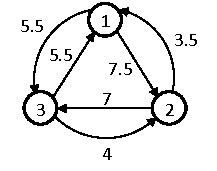
\includegraphics[scale=0.75]{Graficos/fig8_RB}		}{  \caption*{Grafo \(V\)}	}
	%
\end{floatrow}
\end{figure}


\begin{table}[H]
   \fontsize{7}{11}\selectfont
   	\captionsetup{justification=centering, labelfont=footnotesize, font=footnotesize}
    \centering
	\begin{tabular}{c|c} \thickline
    \hline
     Votante &  Preferencia \\ \hline
    \(V_1\) & \(A_1 \succ A_2 \sim A_3\)  \\
    \(V_2\) & \(A_1 \succ A_2 \succ A_3\)  \\
    \(V_3\) & \(A_1 \sim A_2 \succ A_3\)  \\
    \(V_4\) & \(A_1 \succ A_2 \succ A_3\)  \\
    \(V_5\) & \(A_1 \succ A_2 \succ A_3\)  \\
    \(V_6\) & \(A_2 \succ A_3 \succ A_1\)  \\
    \(V_7\) & \(A_2 \succ A_3 \succ A_1\)  \\
    \(V_8\) & \(A_3 \succ A_1 \succ A_2\)  \\
    \(V_9\) & \(A_1 \sim A_2 \sim A_3\)  \\
    \(V_{10}\) & \(A_3 \succ A_1 \succ A_2\)  \\
    \(V_{11}\) & \(A_3 \succ A_1 \sim A_2\)  
	\end{tabular}
\label{tab:B32} 
\end{table}
%

\vspace{-2\baselineskip}

\paragraph{Regla de la Mayoría.}

En la regla de la mayoría, se elige a \(A_i\) como mejor alternativa a \(A_j\) ssi un mayor número de electores prefiere a \(A_i\) sobre \(A_j\) \cite{Dasgupta-2003}.\\


\vspace{1\baselineskip}
\textbf{EJEMPLO 15:} Para el ejemplo 14, las votaciones mayoritarias son: \(A_1 \succ A_2\): 7.5 votos a favor; \(A_2 \succ A_3\): 7 votos a favor; \(A_1 \succ A_3\) y \(A_3 \succ A_1\) 5.5 votos a favor de cada opción, empate. No hay un ganador. Se forman ciclos: \footnote{Un ciclo es una secuencia de proposiciones que inician y terminan con una misma alternativa. En el grafo asociado, un ciclo es un camino cerrado que inicia en un nodo y que regresa al mismo recorriendo el grafo en el sentido de los arcos.} \(A_1 \succ A_2 \succ A_3 \succ A_1\); \(A_1 \succ A_3 \succ A_1\). 

\begin{figure}[H]
\begin{floatrow}
	\fontsize{7}{11}\selectfont
	\captionsetup{justification=centering, labelfont=footnotesize, font=footnotesize}
	%	Tabla
	\capbtabbox{%
	 \begin{tabular}{c|ccc} \thickline
	 & \(A_1\) & \(A_2\) & \(A_3\)    \\ \hline
    \(A_1\) & 0 & 7.5 & 5.5  \\
	\(A_2\) & 0 & 0 & 7  \\
    \(A_3\) & 5.5 & 0 & 0  \\
	\end{tabular}
	}{	  \caption*{Voto mayoritario.}%
	}
	%	Figura
	\ffigbox{	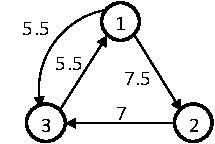
\includegraphics[scale=0.75]{Graficos/fig9_RB}		}{  \caption*{Grafo}	}
	%
\end{floatrow}
\end{figure}
%

\vspace{-1\baselineskip}

\paragraph{Método de Copeland.}

La matriz de pérdidas y ganancias \(R^* = (c_{ij})\) se define por \(c_{ij} = 1\) ssi \(\alpha_{ij} > \dfrac{n}{2}\), \(c_{ij} = -1\) ssi \(\alpha_{ij} < \dfrac{n}{2}\).
El puntaje de Copeland es igual a la suma de la fila de la matriz de pérdidas y ganancias \cite{Conitzer-2012, Levin-1995}. Las alternativas se ordenan en función del puntaje de Copeland. 

\vspace{1\baselineskip} 
\textbf{EJEMPLO 16:} Para el ejemplo 14

\begin{table}[H]
   \fontsize{7}{11}\selectfont
   	\captionsetup{justification=centering, labelfont=footnotesize, font=footnotesize}
    \centering
	\begin{tabular}{c|ccccc} \thickline
    \hline
	 & \(A_1\) & \(A_2\) & \(A_3\) &  & \(C\)   \\ \hline
    \(A_1\) & 0 & 1 & 0 &  & 1 \\
	\(A_2\) & -1 & 0 & 1 &  & 0 \\
    \(A_3\) & 0 & -1 & 0 &  & -1 \\
	\end{tabular}
	\caption*{Matriz Copeland.}
\label{tab:B32} 
\end{table}

El orden agregado es: \(S_c: A_1 \succ A_2 \sim A_3\).

El método puede modificarse al método equivalente: La matriz de Copeland \(R^* = (c_{ij})\) se define por \(c_{ij} = 1\) ssi \(\alpha_{ij} \geq \dfrac{n}{2}\). El puntaje total de la alternativa \(A_i\) es igual a la suma de los elementos de la fila \(i\) menos la suma de los elementos de la columna \(i\) de la matriz \(R^*\). Las alternativas se ordenan en función del puntaje total.

\vspace{1\baselineskip} 
\textbf{EJEMPLO 17:} Continuando con el ejemplo 14:

\vspace{-1\baselineskip}
\begin{figure}[H]
\begin{floatrow}
	\fontsize{7}{11}\selectfont
	\captionsetup{justification=centering, labelfont=footnotesize, font=footnotesize}
	%	Tabla
	\capbtabbox{%
	 \begin{tabular}{c|ccccc} \thickline
	 & \(A_1\) & \(A_2\) & \(A_3\) &  & \(C\)   \\ \hline
    \(A_1\) & 0 & 1 & 1 &  & 1 \\
	\(A_2\) & 0 & 0 & 1 &  & 0 \\
    \(A_3\) & 1 & 0 & 0 &  & -1 \\
	\end{tabular}
	\vspace{0.5em}
	}{	  \caption*{Matriz de Copeland}%
	}
	%	Figura
	\ffigbox{	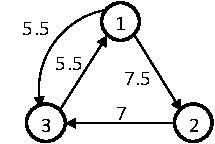
\includegraphics[scale=0.75]{Graficos/fig10_RB}		}{  \caption*{Grafo Copeland}	}
	%
\end{floatrow}
\end{figure}
%

%\vspace{-1\baselineskip}

La relación de Copeland es una forma de expresar la regla de la mayoría. En el grafo de la matriz de Copeland en estricto rigor no se ponderan los arcos; sin embargo, para presentar mayor información, y que quede claro su relación con la regla de la mayoría, se presenta la ponderación de los arcos.

\vspace{-0.5\baselineskip}

\paragraph{Método de Condorcet.}

En el leguaje de Condorcet una <<proposición>> es la comparación de un par de alternativas (por ejemplo, \(A_3 \succ A_2\)) una <<opinión>> es un conjunto de proposiciones. La proposición inversa de \(A_i \succ A_j\) es \(A_j \succ A_i\). Una opinión es <<contradictoria>>, <<absurda>> o <<imposible>> si las proposiciones que la conforman generan un ciclo; una opinión es <<no contradictoria>> si no hay ciclos.

\vspace{1\baselineskip} 
El método de Condorcet consiste en: 
\begin{seriate}
\item Tomar las proposiciones que estén de acuerdo con el mayor número de votantes y analizar si dichas proposiciones no generan ciclos.
\item Si este es el caso, la opinión conformada por estas proposiciones es el orden que está de acuerdo con la mayoría de votantes.
\item Si hay ciclos, se toman las proposiciones que tengan menor votación y se las va borrando sucesivamente hasta eliminar los ciclos.
\item el orden final se construye a partir de las proposiciones remanentes (Young, 1990:28).
\end{seriate}

\vspace{1\baselineskip} 
El método de Condorcet en términos de grafo consiste en verificar si el grafo de la relación de Copeland es acíclico; si ese es el caso, se termina el proceso. Si no es así, hay que borrar los arcos de menor peso consecutivamente hasta obtener un grafo acíclico.

\vspace{1\baselineskip} 
\textbf{EJEMPLO 18:} Para el ejemplo 14, el grafo de la relación de Copeland tiene ciclos. Al aplicar el método de Condorcet nos queda:

\vspace{-1\baselineskip}

\begin{center}
\begin{figure}[H]
	\fontsize{7}{11}\selectfont
	\captionsetup{justification=centering, labelfont=footnotesize, font=footnotesize}
    \centering
    \caption*{Relación de Copeland \(\qquad \qquad  R^* \backslash \{\text{arcos de menor peso}\} \qquad \qquad  \qquad  \mathcal{R}\)}
    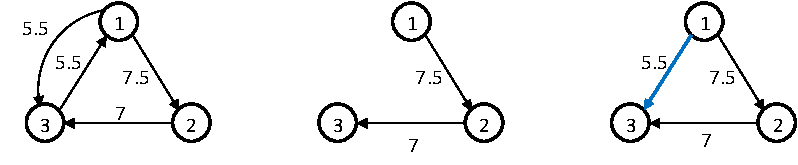
\includegraphics[scale=0.75]{Graficos/fig11_RB}	
    \label{fig:RB_grafo11}
\end{figure}
\end{center}

\vspace{-2\baselineskip}

\paragraph{Método de Borda.}
El método de Borda consiste en:

\begin{APAenumerate}
    \item De acuerdo al criterio de cada votante:
        \begin{seriate}
            \item Ordenar las alternativas descendentemente -de mejor a peor-.
            \item Asignar el valor \(n-1\) a la mejor alternativa, \(n-2\) a la siguiente mejor y así sucesivamente.
        \end{seriate}
    \item Calcular la cuenta o puntuación de Borda sumando los puntajes obtenidos.
    \item El orden resultante se define en función de la puntuación total \cite{Conitzer-2012, Levin-1995}. 
\end{APAenumerate}

El método puede ampliarse para cuando un elector establece empates entre las alternativas. En un primer paso, las alternativas que empatan se ordenan de manera arbitraria; en el segundo paso, el puntaje asignado a todas las alternativas empatadas es el promedio de los puntajes.


\vspace{1\baselineskip} 
\textbf{EJEMPLO 19:} Para la votación del ejemplo 14, tenemos:

\begin{table}[H]
   \fontsize{7}{11}\selectfont
   	\captionsetup{justification=centering, labelfont=footnotesize, font=footnotesize}
    \centering
	\begin{tabular}{c|ccccccccccccc} \thickline
	 & \(C_1\) & \(C_2\) & \(C_3\) & \(C_4\)& \(C_5\)& \(C_6\)& \(C_7\)& \(C_8\)& \(C_9\)& \(C_10\)& \(C_11\)&  & \(B\)   \\ \hline
    \(A_1\) & 2 & 2 & 1.5 & 2 & 2 & 0 & 0 & 1 & 1 & 1 & 0.5 &  & 13 \\
	\(A_2\) & 0.5 & 1 & 1.5 & 1 & 1 & 2 & 2 & 0 & 1 & 0 & 0.5 &  & 10.5 \\
    \(A_3\) & 0.5 & 0 & 0 & 0 & 0 & 1 & 1 & 2 & 1 & 2 & 2 &  & 9.5 \\
	\end{tabular}
	\caption*{Cuenta de Borda}
\label{tab:B32} 
\end{table}

El método de Borda es equivalente a sumar los elementos de las filas de la matriz de votación:

\begin{table}[H]
   \fontsize{7}{11}\selectfont
   	\captionsetup{justification=centering, labelfont=footnotesize, font=footnotesize}
    \centering
	\begin{tabular}{c|ccccc} \thickline
	 & \(A_1\) & \(A_2\) & \(A_3\) &  & B   \\ \hline
    \(A_1\) & 0 & 7.5 & 5.5 &  & 13  \\
	\(A_2\) & 3.5 & 0 & 7 &  & 10.5 \\
    \(A_3\) & 5.5 & 4 & 0 &  & 9.5 \\
	\end{tabular}
\label{tab:B32} 
\end{table}

El orden agregado es: \(S_B : A_1 \succ A_2 \succ A_3\).

\paragraph{Aplicación de los métodos de votación al análisis multicriterio.}

Para aplicar los métodos de votación al análisis multicriterio, primero se debe transformar cada <<criterio>> en un <<voto>>. Una posible forma de hacerlo es considerar un modelo con umbral.

\subparagraph{Modelo con umbral.}

Sean \(x,y \in X = \Re ^n\) dos alternativas, \(c_j\) el umbral de indiferencia asociado al criterio \(x\). La preferencia parcial estricta y la indiferencia parcial se definen por:
\begin{equation*}
\left\{
\begin{aligned}
x \, P_j \, y & \Leftrightarrow x_j > y_j +c_j\\
x \, I_j \, y & \Leftrightarrow |x_j -y_j| \leq c_j
\end{aligned}
\right.
\end{equation*}


\newpage


\textbf{EJEMPLO 20:} Consideremos la siguiente matriz de impacto:

\begin{table}[H]
   \fontsize{7.5}{11}\selectfont
   	\captionsetup{justification=centering, labelfont=footnotesize, font=footnotesize}
    \centering
	\begin{tabular}{l|cccccc} \thickline
	 \multirow{2}{*}{Criterio} 	& \multirow{2}{*}{PIB pc} & \multirow{2}{*}{Inflación} & Consumo & Emisiones  & \multirow{2}{*}{Desempleo} & \multirow{2}{*}{Pobreza}	\\
	 		&		&		&	Energía pc &	 \(CO_2\) pc	 \\     \hline
    Objetivo & \(\max\) & \(\min\) & \(\min\) & \(\min\) & \(\min\) & \(\min\)   \\
	Umbral & 600 & 0.50 & 100 & 200 & 1.50 & 1.50 \\
    \cellcolor{pastelyellow} Ecuador & 7830 & 3.6 & 836.3 & 2111 & 5.0 & 5.48 \\
	\cellcolor{pastelyellow} Colombia & 9000 & 2.3 & 696.3 & 1560 & 11.6 & 9.64 \\
	\cellcolor{pastelyellow} Perú & 8790 & 1.5 & 667.1 & 1646 & 7.9 & 5.00 \\
	\end{tabular}
\label{tab:B32} 
\end{table}

Al aplicar la Definición 1, las relaciones entre las alternativas quedan:

\begin{table}[H]
   \fontsize{7}{11}\selectfont
   	\captionsetup{justification=centering, labelfont=footnotesize, font=footnotesize}
    \centering
	\begin{tabular}{l|c} \thickline
	Criterio & Preferencia  \\ \hline
    PIB pc & \(C \sim P \succ E\)   \\
	Inflación & \(P \succ C \succ E\)   \\
    Consumo Energía pc & \(C \sim P \succ E\)   \\
	Emisiones \(CO_2\) pc & \(C \sim P \succ E\)   \\
	Desempleo & \(E \succ P \succ C\)   \\
	Pobreza & \(P \sim E \succ C\)   \\
	\end{tabular}
\label{tab:B32} 
\end{table}

Que nos lleva a la matriz de <<votación>> siguiente:

\begin{figure}[H]
\centering
\begin{floatrow}
	\fontsize{7}{11}\selectfont
	\captionsetup{justification=centering, labelfont=footnotesize, font=footnotesize}
	%	Tabla
	\capbtabbox{%
	 \begin{tabular}{c|ccccc} \thickline
	 & ECU  & COL & PER & & B   \\ \hline
     ECU  & 0 & 2 & 1.5 & & 3.5   \\
	 COL  & 4 & 0 & 3 & & 7       \\
     PER  & 4.5 & 3 & 0 & & 7.5   \\
	\end{tabular}
	\vspace{1.1em}
	}{	  \caption*{Matriz de votación}%
	}
	%	Figura
	\ffigbox{	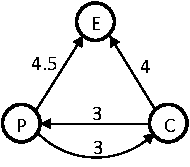
\includegraphics[scale=0.75]{Graficos/fig12_RB}		}{  \caption*{Grafo Copeland}	}
	%
\end{floatrow}
\end{figure}

\vspace{-1\baselineskip}
\[
	\text{Perú} \succ \text{Colombia} \succ \text{Ecuador}
\]

La aplicación del método de Condorcet lleva a soluciones múltiples una de las cuales coincide con el método de Borda:
\begin{align*}
	\text{Perú} \succ \text{Colombia} \succ \text{Ecuador}
\\
	\text{Colombia} \succ \text{Perú} \succ \text{Ecuador}
\end{align*}

\subsubsection{Axiomas de la elección social}

Es bien conocido que Kenneth Arrow dio un tratamiento axiomático a la Teoría de la Elección Social. Arrow primero estableció ciertas condiciones o propiedades (axiomas) razonables que se considera deben cumplir las reglas de agregación de las preferencias, para luego intentar encontrar la regla que satisfaga estos axiomas. Al final Arrow demostró que tal regla no existe \footnote{Erik Maskin (Maskin, 2009:6) al referirse Arrow comenta: Aunque la regla de la mayoría viola la decisión y la regla de la mayoría viola la independencia, Ken pensó que seguramente debe haber otras reglas de votación que satisfacen los cuatro axiomas: decidibilidad, consenso, ausencia de un dictador y la independencia de alternativas irrelevantes. Pero después de probar regla tras regla, con el tiempo llegó a sospechar que estos axiomas son colectivamente contradictorios. Y así es como nació el teorema de imposibilidad, Ken mostró que no hay una regla de votación que satisfaga los cuatro axiomas.}. Sin embargo, al aplicar cualquier método de agregación debería estar claro cuáles propiedades se satisfacen y cuáles no (de acuerdo a Arrow no es posible que se satisfagan todas). Veamos las propiedades de los operadores de agregación.

\vspace{1\baselineskip}
Sea \(\Re\) el conjunto de relaciones de preferencia racionales definidas sobre el conjunto de alternativas \(X = \{A_1,A_2,\dots, A_m\}\). Consideremos el operador \(\mathcal{H}\):
\begin{align*}
\mathcal{H}: \Re ^n & \rightarrow \Re \\
(R_1, R_2, \dots , R_n) & \mapsto R
\end{align*}


Sea \(\Omega = \{1,2,\dots, n\}\) el conjunto de índices de los individuos.

\vspace{1\baselineskip}
Para facilitar el enunciado a algunas de las propiedades veamos una definición previa.
Aumento del grado de preferencia. Se dice que el grado de la preferencia parcial entre \(A_i\) y \(A_j\) aumenta ssi de \(P_k^{-1}\) se pasa a \(I_k\) o \(P_k\), o de \(P_k\) se pasa a \(I_k\): \(P_k: (A_i \, P_k^{-1} \, A_j) \wedge [(A_i \, I'_k \, A_j) \vee (A_i \, P'_k \, A_j)]\) ó \((A_i \, I_k \, A_j) \wedge (A_i \, P'_k \, A_j)\). Para la preferencia agregada el grado de la preferencia entre \(A_i\) y \(A_j\) aumenta ssi de \(P^{-1}\) se pasa a \(I,J\) o \(P\); o de \(J\) se pasa a \(I\) O \(P\); de \(I\) se pasa a \(P\): \((A_i \, P^{-1} \, A_j) \wedge [(A_i \, I' \, A_j) \vee (A_i \, J' \, A_j) \vee (A_i \, P' \, A_j)]\) ó \((A_i \, J \, A_j) \wedge [(A_i \, I' \, A_j) \vee (A_i \, P' \, A_j)]\) ó \((A_i \, I \, A_j) \wedge (A_i \, P' \, A_j)\).

\paragraph{Propiedades de los operadores.}

Se dice que el operador de agregación de preferencias \(\mathcal{H}\) es:

\begin{APAenumerate}
    \item \textbf{Paretiano:} ssi \(\mathcal{H}\) respeta la unanimidad de la preferencia estricta entre las alternativas. O sea, ssi para todos los individuos, la alternativa \(A_i\) es estrictamente preferida a \(A_j\), en la preferencia agregada también; es decir: \(\forall k \in \Omega, A_i \, P_k \, A_j \Rightarrow A_i \, P \, A_j\).
    
   \vspace{1\baselineskip}
    \item \textbf{Fuertemente Paretiano:} ssi para todos los individuos, la alternativa \(A_i\) es débilmente preferida a \(A_j\), y si para algún individuo es estrictamente preferida, en la preferencia agregada también lo es: \(\forall k \in \Omega, A_i \, R_k \, A_j \wedge \exists j \in \Omega,  A_i \, P_j \, A_j \Rightarrow A_i \, P \, A_j\).
    
    \vspace{1\baselineskip}
    \item \textbf{Simétrico entre criterios:} (anónimo) ssi no importa los nombres de los individuos. Es decir, hay un trato igualitario para todos ellos. Esto se estable de la manera siguiente: un cambio de orden entre los criterios no afecta el resultado del funcional. Si \(\sigma\) es una permutación de \(\Omega\), entonces:
    \[
    	\mathcal{H}(R_1, R_2, \dots, R_n) = \mathcal{H}(R_{\sigma (1)}, R_{\sigma (2)}, \dots, R_{\sigma (n)})
    \]
    
    \vspace{1\baselineskip}
    \item \textbf{Neutral entre alternativas:} ssi la preferencia agregada se invierte cuando se invierten las preferencias parciales originales.
    \[
    	\mathcal{H}(R_1^{-1}, R_2^{-1}, \dots, R_n^{-1}) = \mathcal{H}(R_{11}, R_{2}, \dots, R_{n})^{-1}
    \]
    
    \vspace{1\baselineskip}
    \item \textbf{Tiene respuesta positiva:} ssi en la preferencia agregada \(A_i\) es débilmente preferida a \(A_j\) y si aumenta el grado de preferencia parcial \(A_i\) sobre \(A_j\) para algún \(k \in \Omega\), entonces \(A_i\) es estrictamente preferido a \(A_j\). Si \(A_i \, R \, A_j\) y para algún \(k \in \Omega\), \(\{( A_i \, P_k^{-1} \, A_j) \wedge [( A_i \, I'_k \, A_j) \vee ( A_i \, P'_k \, A_j)]\} \vee \{( A_i \, I_k \, A_j) \wedge ( A_i \, P'_k \, A_j)\}\) entonces \(A_i \, P' \, A_j\); donde
\begin{align*}
	R &= \mathcal{H}(R_1, \dots, R_k, \dots, R_n) ,
	\\
	R' &= \mathcal{H}(R_1, \dots, R'_k, \dots, R_n).
\end{align*}
    
    Adicionalmente puede añadirse un axioma adicional relacionado con el axioma de respuesta positiva. 
    
        \begin{APAitemize}
            \item \textbf{No decreciente:} ssi el grado de la preferencia agregada entre \(A_i\) y \(A_j\) no decrece cuando aumenta el grado de preferencia de \(A_i\) sobre \(A_j\) para algún \(k \in \Omega\). Si para algún \(k \in \Omega\), \(\{(A_i \, P_k^{-1} \, A_j) \wedge [(A_i \, I'_k \, A_j) \vee (A_i \, P'_k \, A_j)]\} \vee \{(A_i \, I_k \, A_j) \wedge (A_i \, P'_k \, A_j)\}\)  entonces \((A_i \, I \, A_j) \Rightarrow [(A_i \, I' \, A_j) \vee (A_i \, P' \, A_j)] \vee (A_i \, J \, A_j) \Rightarrow [(A_i \, J' \, A_j) \vee (A_i \, P' \, A_j)] \vee (A_i \, P \, A_j) \Rightarrow (A_i \, P' \, A_j)\); donde \(R = \mathcal{H}(R_1, \dots, R_k, \dots, R_n) \), \(R' = \mathcal{H}(R_1, \dots, R'_k, \dots, R_n)\).
        \end{APAitemize}
    
    \vspace{1\baselineskip}
    \item \textbf{Satisface el axioma de independencia de alternativas irrelevantes:} ssi la relación agregada \(A_i \, R \, A_j\) depende únicamente de las preferencias entre estas alternativas. De manera formal, \(R_k\) y \(R'_k\) son relaciones en \(X\), \(k \in \Omega\), y si \(R_k : \{A_i, A_j\} = R'_k : \{A_i, A_j\}\) para todo \(k \in \Omega\), entonces: \((R_1, R_2, \dots, R_n) : \{A_i, A_j\}  = \mathcal{H}(R'_1,  R'_2, \dots, R'_n) : \{A_i, A_j\} \). \(R : Y\) es la restricción de la relación \(R\) al subconjunto de alternativas \(Y\).
    
    \vspace{1\baselineskip}
    \item \textbf{Dictatorial:} ssi existe un individuo \(k\) llamado dictador tal que la preferencia estricta del dictador determina la preferencia estricta agregada: \(A_i \, P_k \, A_j \Rightarrow A_i \, P \, A_j\).
    
    
    La definición de \(\mathcal{H}\) implícitamente define cuatro condiciones adicionales:
    
    \vspace{1\baselineskip}
    \item \textbf{Universalidad del dominio:} La regla de agregación \(\mathcal{H}\) se aplica a cualquier vector de preferencias racionales \((R_1, R_2, \dots, R_n).\)
    
    \vspace{1\baselineskip}
    \item \textbf{Racionalidad de la relación agregada:} La relación agregada \(R\) es completa, reflexiva y transitiva sobre el conjunto de alternativas \(X\) (es un orden o preorden total o completo).
    
    \vspace{1\baselineskip}
    \item \textbf{Decidibilidad débil:} En cualquier conjunto de alternativas \(X\) puede identificar un elemento máximo.
    
    \vspace{1\baselineskip}
    \item \textbf{Decidibilidad fuerte:} En cualquier conjunto de alternativas \(X\) puede identificar un único elemento máximo.
\end{APAenumerate}

\vspace{1\baselineskip}
\textbf{Observación.} La condición de simetría entre criterios es más general que la condición de no existencia de un dictador. De igual manera, si la relación agregada es un orden o preorden total, se cumple que es decidible fuerte o débil respectivamente.


Como un ejercicio para el lector queda propuesto verificar el cumplimiento de las propiedades de los operadores de agregación de los métodos de votación que se ha mencionado en este documento.

\nocite{Burbano-2014, Burbano-2016, Burbano-2009, Cioni-2010, Colell-1995, Reina-2008}

}

\newpage

% ------------------ Castro ------------------%
\Tutorial{El Arte de hacer Estadísticas: Estadística básica para personas con alma de artista. ¡Desarrolla tu propia encuesta online!}{Gabriela Castro}{Sociedad Ecuatoriana de Estadística, Ecuador}{gaby77castro@gmail.com}{
	\subsubsection{Orígenes de la estadística}

Se puede considerar dos de las actividades que han realizado los seres humanos, como las bases para los orígenes de la estadística, son las siguientes:

\vspace{1\baselineskip}
\textbf{El interés por registrar todo lo que le rodea:} Los seres humanos siempre han estado atentos a su entorno y han buscado registrar lo que está a su alrededor, mediante pinturas rupestres en cuevas, esculpe sobre huesos, madera, tablas de arcilla papiros o papel \cite{Fernandez-2002}.

Los primeros registros se relacionan a actividades de caza, religiosas o guerras; pero a medida que aparecen la primera civilización los registros se convierten en una herramienta necesaria para los Estados, que buscan contar con registros de propiedades, censos de población, transacciones
económicas, disponibilidad de recursos \cite{Fernandez-2002}.

La segunda se relaciona con la \textbf{afición de los seres humanos por los juegos de azar}; esta es una afición surgida desde los comienzos de la humanidad, según se ha encontrado en yacimientos arqueológicos muy antiguos. Esta afición exige buscar la solución más favorable para sus
intereses; es decir, la solución que de brinde mayor probabilidad de éxito \cite{Fernandez-2002}.

\paragraph{Un poco de historia de la Estadística en Ecuador.}

En la \textbf{época incásica} el Tahuantinsuyo habitaba una población estimada en más de 12 millones de personas, que se agrupaban en una multiplicidad de etnias diferente; que, aunque compartían algunos atributos culturales, diferían en otros aspectos como el lenguaje, lo que representaba un problema para el compartir de ideas, tales como la programación de las actividades burocráticas, la administración de los bienes y actividades estatales repartidas por todo el Imperio. 

\begin{wrapfigure}{l}{0.25\textwidth} %this figure will be at the right
    \centering
    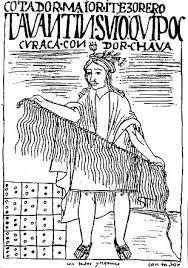
\includegraphics[scale=0.35]{Graficos/fig5_GC.jpg}
\end{wrapfigure}

En este sentido, una de las herramientas más importantes fueron los \textbf{quipus}, proveniente del vocablo quechua que significa <<nudo>> ; se refiere a un implemento de cuerdas anudadas que fue el principal instrumento para registrar información en el Imperio Inca.

A partir de la conquista, los españoles relatan que la información contenida en los quipus incluía datos estadísticos relacionados con el registro de censos, la contabilidad tributaria y otras informaciones numéricas similares. 

\begin{wrapfigure}{r}{0.25\textwidth} %this figure will be at the right
    \centering
    
\includegraphics[scale=0.35]{Graficos/fig3_GC.jpg}
    \vspace{-2em}
\end{wrapfigure}

En la \textbf{época colonia}, en las últimas décadas del siglo XVIII, comenzó un proceso de recolección de información que la Corona española requería de sus posesiones americanas. Es así que los ministros en cada uno de sus ramos respectivos, comenzaron a utilizar la frase \textquote{Su majestad quiere saber}, a fin de recabar toda esa información necesaria para planificar correctamente un futuro de seguridad y promisión para los territorios americanos. A fines del siglo XVII, se comenzó a utilizar la frase: \textquote{Su Majestad quiere una exposición clara y sencilla}.

\vspace{1\baselineskip}
La cantidad de información almacenada sin revisar y su escasa utilización dieron muestra del poco interés que demostraron los políticos y funcionarios de esa época, y es solo a finales del siglo XX cuando se comienza a valorar este bagaje de información.

\begin{wrapfigure}{l}{0.35\textwidth} %this figure will be at the right
    \centering
    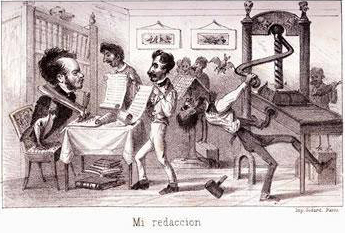
\includegraphics[scale=0.3]{Graficos/fig1_GC.jpg}
\end{wrapfigure}

Durante la \textbf{época republicana}, se hicieron intentos de institucionalizar la ejecución de de censos a través de la expedición de leyes o decretos que permitieran su realización, normas legales que se han perdido o se encuentran dispersas entre gran cantidad de archivos históricos de nuestro país. 

\vspace{1\baselineskip}
Así, por ejemplo, en la Primera Constitución del Estado del Ecuador de 1830, al disponerse que la representación de diputados de los tres departamentos (Azuay, Guayas y Quito) que conformaron el <<Estado del Ecuador>>, se la haría según el censo de población; en 1873 el presidente García Moreno decretó la creación de una Oficina de Estadística, en la ciudad de Quito; durante la presidencia de Velasco Ibarra, en 1970, se decreta que las funciones de Estadísticas y Censos serán ejercidas a través del Instituto Nacional de Estadísticas (INE). Finalmente, en 1976 y en 1978, se expide la Ley de Estadística, vigente hasta esta fecha, en la que se crean el Sistema Estadístico Nacional (SEN), el Consejo Nacional de Estadística y Censos (CONEC) y el Instituto Nacional de Estadística y Censos (INEC).

\vspace{1\baselineskip}
En la \textbf{actualidad}, esta ciencia es tiene gran aplicabilidad, hasta el punto de no concebir un trabajo de carácter científico sin el apoyo de algún método estadístico. 

\begin{wrapfigure}{r}{0.25\textwidth} %this figure will be at the right
    \centering
    
\includegraphics[scale=0.12]{Graficos/fig9_GC.jpg}
    \vspace{-1em}
\end{wrapfigure}

Se ha convertido en un elemento fundamental de la sociedad de la información y del conocimiento, en la cual se desarrolla el mundo y el Ecuador.

El Ecuador se ha avanzado en cuanto a la generación de información estadística, se cuenta con un Instituto Nacional de Estadística más fortalecido; así como el Banco Central de Ecuador, encargado de la generación de las estadísticas de síntesis de los principales sectores de la economía; el país cuenta con el Sistema Nacional de Información a cargo de la Secretaría Nacional de Planificación y Desarrollo. Sin embargo, es innegable que en nuestro medio existe un vacío notorio en lo referente a la evolución de la estadística, debido a falta de obras que recojan y organicen la información dispersa y proporcionen una amplia y selecta bibliografía como fuente de consulta.

\vspace{1\baselineskip}
En el país existen diversas situaciones que impiden el desarrollo de las actividades estadísticas, a la par de las tendencias de los países más desarrollados, tales como: escaso financiamiento, la falta consciencia por parte de los gobernantes sobre la importancia de la estadística para la toma de decisiones, la falta de cultura estadística nacional de productores, informantes y usuarios, la limitada armonización e integración de la información, la falta de decisión política y la falta de capacitación del personal involucrado el trabajo estadístico.

\subsubsection{¿Qué es la Estadística?} 

La estadística es una ciencia teórica que forma parte de las ciencias matemáticas; facilita la toma de decisiones mediante la presentación ordenada de los datos a través de tablas y gráficos estadísticos; también permite reducir los datos observados a un pequeño número de medidas estadísticas que permitan la comparación entre diferentes series de datos; además, permite estimar la probabilidad de éxito que tiene cada una de las decisiones posibles \cite{Fernandez-2002}.

\paragraph{Ramas de la estadística.}

La estadística se puede dividir en dos ramas principales, la estadística descriptiva y la estadística analítica:

\vspace{1\baselineskip}
La \textbf{estadística descriptiva} tiene como objeto representar y resumir los resultados, \([...]\) En general se condensa la información obtenida, en tablas, gráficos y parámetros que la resumen y permiten entenderla rápidamente \cite{Vargas-1995}. <<La reducción de datos conlleva a un error que debe ser controlado, puede realizarse previamente durante el proceso de tabulación o, con mayor eficacia, utilizando las medidas estadísticas>> \cite{Fernandez-2002}, las mismas que permitirán comparar diferentes series de datos obtenidas mediante diversas observaciones.

La \textbf{estadística analítica}, también denomina inferencial, estudia los elementos de una muestra y a través de la construcción de un modelo matemático infiere las propiedades a la población muestreada. Estudia la probabilidad de éxito de diferentes soluciones posibles a un problema de las diferentes ramas de la ciencia.

\subsubsection{Conceptos básicos de la estadística}

\textbf{Población:} Cualquier conjunto de personas, objetos, ideas, o acontecimientos que se someten a una observación estadística de una o varias características que comparten sus elementos y que permiten diferenciarlos. El significado de población en la estadística es más amplio que el utilizado en el lenguaje común, que suele hacer alusión al conjunto de personas.

\textbf{Elementos o individuos de una población:} son cada uno de los componentes de la población.

\textbf{Tamaño de la población:} es el número de elementos de una población, que puede ser finito o infinito.

\textbf{Caracteres de una población:} son cada una de las propiedades, rasgos, o cualidades que poseen los elementos de una población.

\textbf{Variable:} es cualquier carácter de una población susceptible de tomar valores numéricos; en todos los elementos de una población no se presenta la misma intensidad de cada uno de dichos valores.

Las variables se clasifican en continuas y discretas, según admitan o no infinitos valores intermedios entre dos valores próximos respectivamente.

\textbf{Muestra:} es la parte seleccionada de una población, en la que los elementos que son parte, no tiene ninguna característica esencial que los distinga del resto. Se utiliza cuando se pretenden contar con una parte representativa de la población.

\textbf{Censos:} son observaciones exhaustivas que estudias los caracteres estructurales y estáticos de toda una población.

\textbf{Encuestas:} son investigaciones realizadas sobre un subconjunto de la población, generalmente son realizadas sobre fenómenos más dinámicos de la población; los datos se obtienen. 

\textbf{Frecuencia:} es el número de repeticiones que presenta un determinado dato de un carácter en los diferentes elementos de una población o muestra.

\textbf{Frecuencia absoluta:} es el número de repeticiones de un determinado valor de una variable. También representa el número de elementos de la población que tiene el mismo valor o modalidad. La suma de frecuencias corresponde al tamaño de la población.

\textbf{Frecuencia relativa:} es una proporción entre el número de veces que se repite un dato y el tamaño de la población. Se obtiene de dividir la frecuencia absoluta de un determinado dato entre el tamaño de la población.  

\subsubsection{Tipos de medidas de los datos}

\textbf{Medida Nominal (datos categóricos):} se refiere a caracteres cualitativos o atributos, no tienen ninguna relación de orden, no puede medirse en una escala continua. Por ejemplo, los colores de cabellos, sexo, sabores de helados, etc.

\textbf{Medida ordinal (datos de tipo ordinal):} en este caso son caracteres cualitativos, pero que tienen una relación de orden; no puede fijarse una distancia entre dos datos consecutivos. Por ejemplo, los niveles educativos, las categorías laborales de una empresa.

\textbf{Medidas cuantitativas o de intervalo:} los datos tienen un orden, es posible medir la distancia entre dos valores cualquiera, pueden ser variables descritas, como número enteros o continuas cuando hay infinitos número en sus intervalos. Por ejemplo, la temperatura, la edad, el salario,
el peso corporal.

\subsubsection{Medidas de posición}

Las medidas de posición representan puntos de referencia que permiten ubicar la situación de una variable estadística en la recta real y de este modo mostrar la síntesis de toda la información contenida en la distribución de frecuencias.

\textbf{Moda:} identifica el valor o intervalo que más se repite, es el valor que se ha observado un mayor número de veces (Casares. 2007).

Se debe tener precaución con el valor modal, puesto que puede ser engañoso, ya que no necesariamente indica la ubicación de la mayoría de los valores de la distribución en su conjunto (Casares. 2007).

\textbf{Medidas de tendencia central}

Las medidas de tendencia central muestran la localización o posición de los valores alrededor de los cuales fluctúan los demás \cite{Vargas-1995}.

\textbf{Media o promedio} se define como la división entre la suma de los valores que toma una variable respecto al total de elementos de una muestra. Se representa con el símbolo , se calcula con la siguiente fórmula \cite{Vargas-1995}:   
\[
	\bar{x}= \dfrac{1}{n} \sum \limits_{i=1}^{n} x_{i} = \dfrac{x_{1}+x_{2}+ \cdots+x_{n}}{n}
\]

Donde:
\begin{APAitemize}
\item \(\bar{x}\): es el valor promedio de la variable.
\item \(x_{i}\): son los valores que toma el elemento \(i\) de la variable.
\item \(n\): es el total de elementos de una muestra.
\item \(\sum\): es la sumatoria.
\end{APAitemize}

\vspace{1\baselineskip}
\textbf{Mediana:} es el dato que se encuentran en el lugar central de un conjunto de datos ordenados. 



\newpage



\subsubsection{Medidas de dispersión}
Las medidas de dispersión permiten evidenciar que tan alejados se encuentran los datos de la media.

\vspace{1\baselineskip}
\textbf{Desviación media:} Es la división entre la suma de los valores absolutos de las diferencias entre cada uno de los valores y el promedio respecto al total.
\[
	D_{m}= \sum_{i=1}^{n} \dfrac{|x_{i} \cdot \bar{x}|}{n}
\] 

\textbf{Varianza muestral:} es el promedio de las diferencias cuadráticas de los datos respecto al promedio; y sus unidades son las unidades de los datos al cuadrado. Su fórmula es la siguiente \cite{Vargas-1995}:
\[
	S^{2}= \sum_{i=1}^{n} \dfrac{ \left( x_{i}-\bar{x} \right)^{2}}{n-1}
\]

\textbf{Desviación estándar:} es la raíz cuadrada de la varianza. Las unidades de medida de la desviación típica son las mimas que la de los datos sobre los que ha sido calculada.
\[
	S= \sqrt{ \sum_{i=1}^{n} \dfrac{ \left( x_{i}-\bar{x} \right)^{2}}{n-1} }
\]


\subsubsection{Representaciones gráficas}

Un gráfico proporciona una impresión que ayuda a clasificar la variabilidad y simetría de los datos. Existen diferentes tipos de gráficos que dependen de la naturaleza del tipo de la variable que se esté analizando.

\begin{table}[H]
\fontsize{7}{11}\selectfont
  \centering
    \begin{tabular}{c | p{9em} | c} \thickline
    	\textbf{Tipo de variable} & \textbf{Gráfico} & \textbf{Representación} \bigstrut\\ \hline
    	Cualitativa & Diagrama de rectángulos o Barras & \raisebox{-\totalheight}{
\includegraphics[width=3cm]{Graficos/fig2_GC.jpg}} \\
        & Sectores o pasteles &  \raisebox{-\totalheight}{
\includegraphics[width=3cm]{Graficos/fig11_GC.jpg}} \\
    \thickline
    \end{tabular}
\end{table}

\begin{table}[H]
\fontsize{7}{11}\selectfont
  \centering
    \begin{tabular}{c | p{9em} | c} \thickline
    \multicolumn{1}{p{7.5em}|}{} & Pictogramas & \raisebox{-\totalheight}{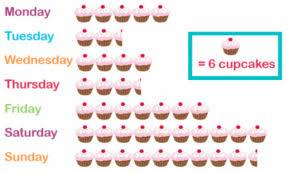
\includegraphics[width=3cm]{Graficos/fig7_GC.jpg}} \\          
          & Perfil radial & \raisebox{-\totalheight}{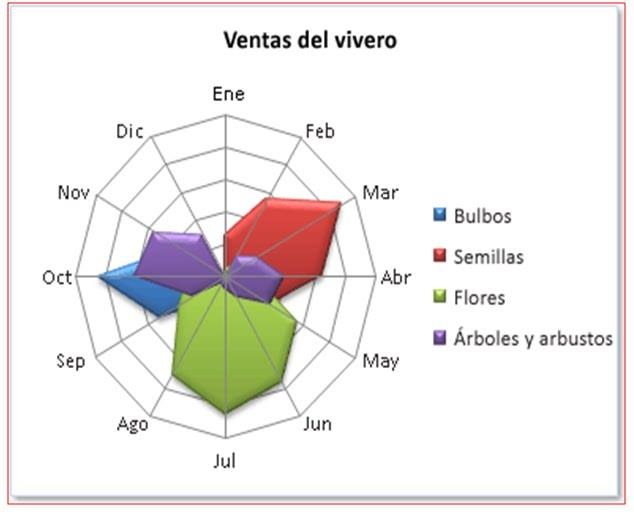
\includegraphics[width=3cm]{Graficos/fig10_GC.jpg}} \\
          & Cartograma & \raisebox{-\totalheight}{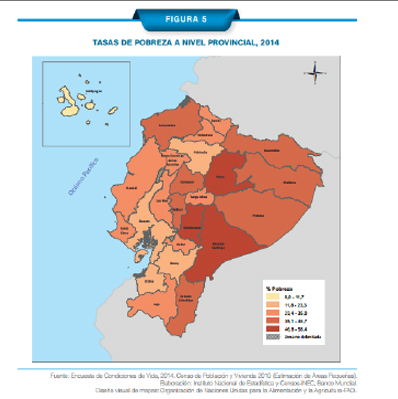
\includegraphics[width=3cm]{Graficos/fig12_GC.jpg}} \\
    \thickline
    \end{tabular}
    \end{table}
    
\begin{table}[H]
\fontsize{7}{11}\selectfont
  \centering
    \begin{tabular}{c | p{9em} | c} \thickline
    \textbf{Tipo de variable} & \textbf{Gráfico} & \textbf{Representación} \bigstrut\\ \hline
    {Cuantitativa} & Histograma & \raisebox{-\totalheight}{
\includegraphics[width=3cm]{Graficos/fig6_GC.jpg}} \\
	& Polígono de \newline frecuencias simples &  \raisebox{-\totalheight}{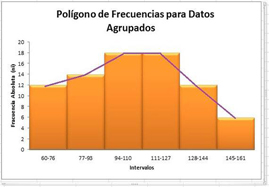
\includegraphics[width=3cm]{Graficos/fig8_GC.jpg}}\\
    & Diagrama de\newline frecuencias acumuladas \newline Variables discretas &  \raisebox{-\totalheight}{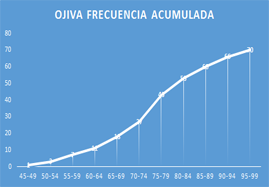
\includegraphics[width=3cm]{Graficos/fig31_GC.png}} \\
    \thickline
    \end{tabular}
\end{table}




\subsubsection{¿Cómo hacer una encuesta?}

La gran mayoría de oficinas de estadística del mundo se rigen por el modelo de producción estadística para la generación de operaciones estadísticas, que <<se define como el conjunto de actividades que involucran, de acuerdo a su naturaleza, la ejecución de las fases y procesos del Modelo Genérico de Producción Estadística. Los procesos incluyen la planificación, diseño, construcción, recolección, procesamiento, análisis, difusión y evaluación de los resultados estadísticos sobre determinada área o tema de interés nacional>> (IENC, 2014). Las encuestas, censos, estadísticas con base en registros administrativos son operaciones estadísticas.

El modelo de producción estadística es un proceso que determina las fases que se deben seguir para implementar una operación estadística. El modelo está diseñado para ser implementado independientemente del tipo de fuente de datos utilizada para la generación de estadísticas. Para Ecuador, este modelo fue desarrollado por el Instituto Nacional de Estadística y Censos; consta de ocho fases y dos macro procesos transversales.

Se presenta a continuación, de manera sucinta las ocho fases del Modelo de Producción Estadística y las actividades que conllevan cada una de ellas.

\begin{figure}[H]
	\fontsize{7}{11}\selectfont
	\captionsetup{justification=centering, labelfont=footnotesize, font=footnotesize}
\caption*{Modelo de producción estadística}
\centering
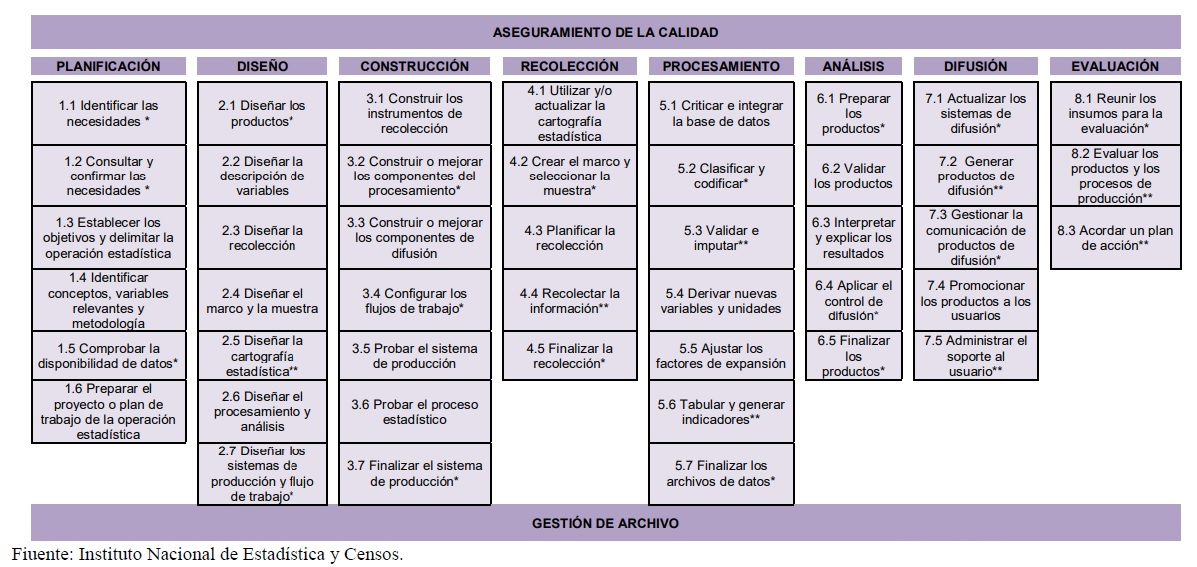
\includegraphics[scale=0.35]{Graficos/fig14_GC.jpg}
\end{figure}

\subsubsection{Desarrollo de encuestas en línea}
En la actualidad el mundo está cada vez más sumido en la tecnología, el uso de los dispositivos tecnológicos es cada vez más común y se usa sin diferencia de edad o estrato social. La sociedad, cada vez más, está automatizando todas las actividades que se realizan a diario, sea a la hora de estudiar, trabajar, o actividades cotidianas.

En este sentido las técnicas para recabar datos se están volcando a la utilización de herramientas tecnológicas, como los dispositivos móviles (tablet, laptop, celulares) y los computadores; otorgando a cada persona que las usa, una rapidez mayor. En tal sentido, se han convertido en una forma, cada vez más utilizada, para levantar información. Aunque cabe destacar que los procesos presenciales para recopilar información no han dejado de estar vigentes.

Este tipo de herramientas son comúnmente utilizadas en el marketing digital, estudios de mercado, puesto que las empresas consideran que las encuestas online son un medio adecuado para evaluar los niveles de satisfacción mediante la web. Por ejemplo, a través de encuestas se evalúan los productos que los consumidores creen mejor que otros o la calidad de los mismos y a partir de dicha información los analistas tiene elementos paras crear estrategias que puedan ser de beneficio para una institución.


	\begin{center}
	\fontsize{7}{11}\selectfont
	\begin{tabularx}{\textwidth}{X X}
		\thickline
		\textbf{Ventajas} & \textbf{Desventajas} \\	\hline
Son económicas, existe mucho ahorro en contratación de encuestadores, desarrolladores de aplicativos para la recolección de datos, entre otros. & Puede existir desconfianza del encuestado, lo que promovería que las respuestas no sean totalmente ciertas. \\
Se obtienen resultados de manera más rápida, al tener automatizado el ingreso de los datos a través de las aplicaciones web. & Sesgo en los resultados, es decir, análisis que se realice, no se podrá inferir sobre el total del universo, ya que no se puede conocer qué porcentaje representa la muestra y si este es suficiente, como para ser considerado.\\
    Aportan valor, porque al hacer una encuesta a los clientes, por ejemplo, al terminar un proceso de compra, demuestra la preocupación por el trabajo bien hecho. & Baja fiabilidad estadística, al no tener un universo conocido y una muestra representativa, los indicadores estadísticos no siempre funcionan con el nivel de fiabilidad requeridos. \\
		\thickline
		\\[3em]
	\end{tabularx}
	\label{tab:B1}

	\emph{Ventajas y desventajas de las encuestas Online}
	\end{center}


\textbf{Nota importante:} Si se quiere usar una encuesta online, generando datos cuantitativos, es necesario respetar y analizar los porcentajes que se obtienen, como porcentajes sobre el total de respuestas, no sobre la población que se está estudiando.

\vspace{1\baselineskip}
Hoy en día existen varias herramientas web a través de las cuales se pueden elaborar encuestas en línea, tales como:

\vspace{1\baselineskip}
\textbf{Google.}
La empresa de google tiene el servicio de encuestas por medio de sus productos de google drive, que permite, de manera gratuita, crear formularios de encuestas, mostrando diferentes plantillas o se crear una propia. Esta herramienta permite analizar los datos luego de ser obtenidos, al crear una base de datos con la información se va recopilando.

\textbf{TypeForm.}
Es un sitio web que ofrece la vista adecuada para las encuestas, el principal interés es que el usuario no abandone el proceso de la encuesta ya sea por las aburridas preguntas o una vista que no le agrada; busca que el internauta observe la encuesta sin importar las preguntas.

\textbf{Survio.}
Es una herramienta bastante popular, que cuenta con un repertorio de 100 platillas o más para emplear. Tiene las opciones de compartir en las redes sociales y ofrece características para evaluar el mercado de comercio entre las empresa.

\textbf{Polldady.}
Es una herramienta que permite crear encuestas on line con la ayuda de un editor visual, de arrastrar y soltar, destaca por la elegancia de sus estilos visuales, las matrices de preguntas y la posibilidad de trabajar con contenido multimedia propio.

\vspace{1\baselineskip}
En este documento nos centraremos en el desarrollo de encuestas con Google Drive, sus ventajas son:

\begin{APAitemize}
\item Costo <<cero>>, por ser gratuito.
\item Se puede obtener respuestas, visualizar estadísticas y obtener resultados a tiempo real.
\item Permite organizar los formularios de manera totalmente personalizada: con logotipo de la empresa, añadiendo imágenes, vídeos, podcast. 
\item Es muy poco intrusivo. La persona encuestada puede elegir contestar cuando lo desee.
\item Se puede segmentar; esto es, si se cuenta con una base de datos, es posible enviar diferentes tipos de encuestas según la edad, sexo, localización, poder adquisitivo.  
\item Las encuestas se recopilan automáticamente generando estadísticas para facilitar la obtención de resultados y su posterior análisis.
\item Los encuestados pueden responder de manera instantánea ya sea desde el ordenador, móvil o tablet.  
\end{APAitemize}

\paragraph{Desarrollo de un formulario Online en Google Drive.}

Para el desarrollo de un formulario online se siguen los siguientes pasos:

\begin{APAenumerate}
\item Acceder a una cuenta de Google. 
\item Ir a la opción Google drive y seleccionar el apartado de formularios. 
\item Diseñar la encuesta.

\subitem Poner el título de la encuesta 
\subitem Se debe elegir el tipo de pregunta que se requiere hacer; estas pueden ser: de texto, respuesta única, respuesta múltiple, selección de una opción de una lista.
\subitem Luego se poner <<Agregar elemento>> y se continúa añadiendo preguntas. 
\subitem En la barra superior del área de trabajo dar click en <<Ver el formulario publicado>> para ver cómo está quedando el formulario.

\item Una vez terminado dar click en <<Enviar formulario>> y se abrirá una nueva ventana con diversas opciones para distribuir el formulario, sea este mediante redes sociales, correo electrónico, vincularlo a un sitio web. 
\end{APAenumerate}

\subsubsection{Visualización de la información}
En este mundo cambiante, lleno de imágenes, es importante la forma en la que la información se presenta. Es por esto, que se han desarrollado varias herramientas online para crear infografías que permitan mostrar los resultados de una manera más atractiva al público en general, y que sea más fácil de comprender y digerir.

Entre los sitios web más conocidos para la creación de infografías se tiene:

\vspace{1\baselineskip}
\textbf{Canva.}
La herramienta de creación de infografías en Canva contiene cientos de elementos de diseño  gratuitos, lo que permite experimentar con la visualización de datos con mucha versatilidad.

\textbf{Info.gram.}
Es una herramienta gratuita que permite insertar información en cada una de las cajas predeterminadas, se puede añadir y eliminar cajas. Se puede elegir más de una docena de opciones gráficas, añadir cajas de texto, fotos, mapas o incluso videos. Es posible compartir la infografía en redes sociales o usar el código para ponerla en un sitio Web.

\textbf{Google Developers.}
Esta es una herramienta de Google, fácil de utilizar y además gratuita. Se puede elegir entre una amplia variedad de gráficos y, que permite conectarlos con los datos generados en tiempo real por una web.

\textbf{Piktochart.}
El editor de Piktochart permite modificar el color de las fuentes, insertar gráficos y cargar formas e imágenes. Es sencillo alinear los diferentes elementos gráficos que integran la infografía y modificar el tamaño de las imágenes de manera proporcional.

\vspace{1\baselineskip}
\textbf{Ejemplo de una infografía:}

\begin{figure}[H]
\fontsize{7}{11}\selectfont
\captionsetup{justification=centering, labelfont=footnotesize, font=footnotesize}
\centering
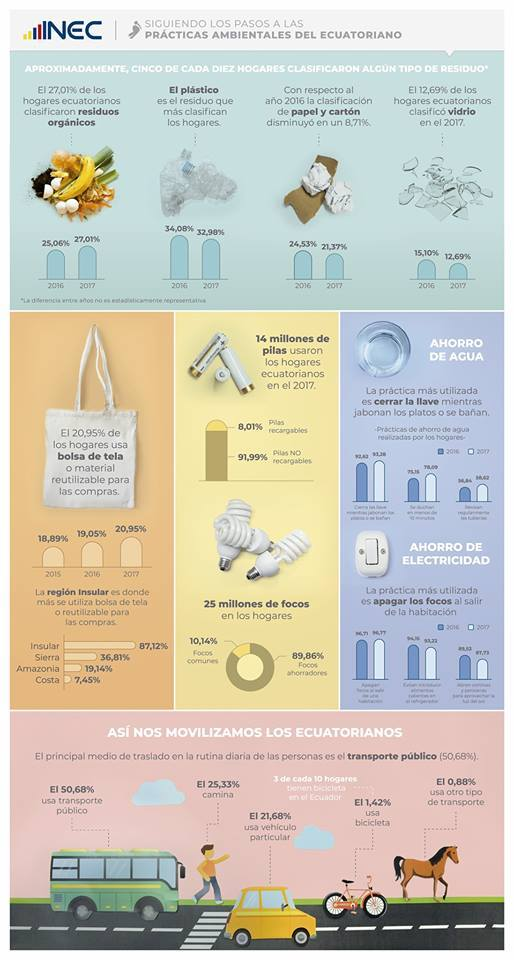
\includegraphics[scale=0.39]{Graficos/fig4_GC.jpg}
\caption*{Fuente: Instituto Nacional de Estadística y Censos}
\end{figure}


\nocite{Caceres-2007, Arribas-2014, CaceresH-2007, INEC-2014, Ross-2007}
}

%
%
%
%
%
%
%
%
%
%
%
%
%
%
%
%
%
%
%
%
%
%
%
%
%
%
%
%
%
%
%
%
%
%


\newpage


% ------------------ Echeverría ------------------%
\Tutorial{Muestreo aleatorio simple muestreo sistemático}{Carlos Echeverría}{\EPN, Ecuador}{carlos.echeverria@epn.edu.ec}{%
\subsubsection{Definiciones fundamentales}\setcounter{figure}{0}

\neodefi{Fenómeno aleatorio y fenómeno no determinístico:}
	Se llama fenómeno \emph{\textbf{determinístico}} o \emph{\textbf{no aleatorio}} a todo fenómeno del cual se obtiene el mismo resultado cuando se realiza bajo iguales condiciones; por ejemplo, un auto demorará el mismo tiempo todas las veces que recorra la misma distancia, con igual velocidad.
	
	Se llama fenómeno \emph{\textbf{no determinístico}} o \emph{\textbf{aleatorio}} a todo fenómeno del cual no necesariamente se obtiene el mismo resultado cuando se realiza bajo las mismas condiciones; por ejemplo, al lanzar una moneda, las ocurrencias de cara y sello se obtienen de manera no predecible. Estos fenómenos son el objeto de estudio de la Estadística y de la Probabilidad.
	
\neodefi{Población:}
	Conjunto formado por todos los posibles elementos concebibles (o hipotéticamente concebibles) que intervienen en el estudio. 
	
	En las poblaciones infinitas no es posible observar todos sus elementos; las poblaciones finitas tienen un número determinado de elementos. 

\neodefi{Variable:}
	Característica de la población a ser estudiada en el proceso. 	Las variables estadísticas pueden ser cuantitativas y cualitativas, donde las cuantitativas pueden ser continuas o discretas, mientras que las cualitativas pueden ser nominales o jerarquizadas.
 
\neodefi{Dato:}
	Valor de la variable que se obtiene de un elemento de la población.
 
\neodefi{Variable cuantitativa continua:}
	Implica procesos de medición. Puede asumir cualquier valor en un intervalo. Los datos que se obtienen se denominan datos continuos. 
 
\neodefi{Variable cuantitativa discreta:}
	Implica procesos de conteo. Toma valores separados. Los datos que se obtienen se denominan datos discretos.
 
\neodefi{Variable cualitativa nominal:}
	Implica determinación de categorías. Los datos se obtienen luego de determinar cada una de las posibles categorías.
 
\neodefi{Variable cualitativa jerarquizada:}
	Implica asignación de un orden. Los datos se obtienen luego de determinar cada una de las posibles jerarquizaciones.

\neodefi{Muestra:}
	Es común utilizar la palabra \emph{\textbf{muestra}} para identificar dos conceptos:
	\begin{seriate}
		\item	Como subconjunto de la población; es decir, el conjunto de elementos de la población que aportan con los datos respecto a la variable en estudio.
		\item	Como el conjunto de datos obtenidos de la variable en un subconjunto de la población.
	\end{seriate}
	
\neodefi{Parámetro:}
	Valor numérico que identifica alguna de las características de la variable en la población. 
	
\neodefi{Estimador:}
	Expresión matemática que especifica cómo utilizar los datos de la muestra para estimar un parámetro. 
	
\neodefi{Estimación:}
	Valor numérico que estima al parámetro; se obtiene al reemplazar los datos de la muestra en el estimador. 
	
\neodefi{Censo:}
	Cuando en el estudio intervienen todos los elementos de la población.
	
\neodefi{Muestreo:}
	Comprende el estudio del instrumento con el cual se van a obtener los datos, el método con el cual se van a seleccionar los elementos que conformarán la muestra y el tamaño de la muestra. 
	
\neodefi{Muestreo aleatorio simple:}
	Si la variable es \emph{\textbf{discreta}}, una \emph{\textbf{muestra aleatoria simple}} o muestra aleatoria irrestricta es aquella en la cual todos los elementos de la población tienen la misma probabilidad de ser incluidos en la muestra.
	
	Si la variable es \emph{\textbf{continua}}, una muestra \emph{\textbf{aleatoria simple}} o muestra aleatoria irrestricta es aquella en la cual la probabilidad de incluir cualquier intervalo de valores en la muestra es igual al porcentaje de la población que está comprendida en dicho intervalo.
	
	El cálculo del tamaño de la muestra depende del tipo de parámetro que se desea estimar, de la variabilidad del proceso, del tipo de población finita o infinita, del comportamiento de la variable y del error de estimación permitido.
	
\neodefi{Muestreo por estratos:}
	Método de muestreo en el cual la población se organiza en grupos llamados estratos. 
	
	Dentro de cada estrato, sus elementos no son relativamente muy diferentes respecto a la variable en estudio; las diferencias son significativas entre elementos que se encuentran en diferentes estratos.
	
	El cálculo del tamaño de la muestra depende del tipo de parámetro que se desea estimar, de la variabilidad del proceso dentro de cada uno de los estratos, del tipo de población finita o infinita, del comportamiento de la variable y del error de estimación permitido. 
	
\neodefi{Muestreo por conglomerados:}
	Método de muestreo en el cual se organiza la población en grupos internamente heterogéneos, llamados conglomerados. Cada conglomerado es muy similar a la  población, respecto a la variable en estudio, se puede considerar como la población en pequeño.
	
	El cálculo del tamaño de la muestra depende del tipo de parámetro que se desea estimar, de la variabilidad del proceso dentro de cada uno de los conglomerados, del tipo de población finita o infinita, del comportamiento de la variable y del error de estimación permitido.
	
\neodefi{Muestreo sistemático:}
	Método de muestreo por medio del cual se obtienen los elementos de la muestra a intervalos uniformes de tiempo, orden o espacio.
	
	Se escoge un número aleatorio que indica el primer elemento de la muestra, un segundo número aleatorio indica cada cuántas unidades (ej. cada cuánto tiempo) se toman los siguientes elementos de la muestra. Para evitar posibles efectos cíclicos que conduzcan a muestras con mayor o menor número de elementos con características que no reflejan lo que realmente sucede en la población, es conveniente cambiar permanentemente el proceso seguido, utilizando números aleatorios.
	



%
%%%%
%%%%%%%%
\subsubsection{Planificación y organizaciión de procesos de muestreo}
	
Se supone que se ha identificado el problema a ser resuelto, su naturaleza y sus aspectos más importantes.

\neodefi{Finalidad:}

El uso que tendrá la información que se obtenga, ¿Para qué?
	
\neodefi{Objetivos:}
	Es indispensable determinar los objetivos que se desean alcanzar, a más de determinar el alcance del estudio, permiten lograr un diseño óptimo.
	
	Se deben determinar los objetivos generales y específicos con explicaciones y justificativos a cada uno de ellos.
	
	Los objetivos generales proporcionan el alcance del estudio, sin determinar las variables que serán motivo de estudio.
	
	Los objetivos específicos definen cada una de las variables motivo de estudio, justificando su inclusión en el proceso.
	
\neodefi{Alcance:}
	Se refiere al alcance geográfico y al nivel de desagregación de la información
	
	El alcance geográfico hace referencia a los lugares o zonas donde se realizará la investigación, que deben estar perfectamente definidos: ciudades, zona urbana o rural, polos de desarrollo económico, regiones administrativas.
	
	Los niveles de desagregación determinan los niveles de detalle con los que se desea obtener la información. Por ejemplo, nivel de instrucción académica por edades, por género, por situación económica, por razas, por regiones.

\neodefi{Variables:}
	Se deben determinar todas las variables que intervendrán y serán cuantificadas en el estudio, jerarquizándolas en orden de importancia para el estudio. Por ejemplo, uso de drogas psicotrópicas en los centros de reclusión considerando edad, género, nivel de instrucción académica, nacionalidad.

\neodefi{Información previa:}
	Se debe conocer la bibliografía con la que se cuenta; estudios similares realizados, en ejecución, planificados u organizados; recursos humanos conocedores de los temas a ser tratados.

\neodefi{Recursos:}
	Se debe determinar específicamente los recursos con los que se cuenta: humanos, físicos, materiales, financieros, tiempo con la respectiva planificación de utilización en las diferentes etapas de la investigación.
	
\neodefi{Cuestionario:}
	Es el instrumento que permite recoger la información, en el cual están reflejados los objetivos específicos a través de preguntas que por su presentación y redacción deben permitir al entrevistador obtener la información propuesta necesaria. Para su elaboración es necesario considerar los siguientes aspectos:
	
	\vspace{0.75\baselineskip}
	\textbf{Criterios para la construcción de cuestionarios}
	
	\begin{APAitemize}
		\item Utilizar el lenguaje más apropiado para alcanzar una comunicación completa y precisa con el entrevistado,
		\item las preguntas deben tener una estructura tal que no permite sugerencias de respuesta al  entrevistado,
		\item cada pregunta debe manifestar claramente solo una idea, sin posibilidad de ambigüedad,
		\item se debe procurar exista secuencia lógica entre las diferentes preguntas,
		\item para cada pregunta debe estar claramente estipulado la escala dentro de la cual contesta el entrevistado.
	\end{APAitemize}
	
	\vspace{0.75\baselineskip}
	\textbf{Validación del cuestionario}
	
	Se busca comprobar la bondad, pertinencia y calidad del cuestionario:
	\begin{APAitemize}
		\item Comprobación del cumplimiento de los objetivos de la investigación,
		\item orden secuencial de las preguntas,
		\item la presentación como colaboradora del proceso de motivación del entrevistador al entrevistado para que conteste con interés y correctamente,
		\item extensión del cuestionario (número de preguntas),
		\item determinación del tiempo promedio empleado por el entrevistado en la contestación completa del cuestionario,
		\item construcción y ubicación correcta de las diferentes alternativas de respuesta, especialmente en el caso de preguntas abiertas.
	\end{APAitemize}
	
	\vspace{0.75\baselineskip}
	Es conveniente realizar pruebas preliminares de contestación del cuestionario por parte de personas que no conocen el proceso, para identificar posibles dificultades en los aspectos expuestos.
	
	\vspace{0.75\baselineskip}
	\textbf{Instrucciones}
	
	Es indispensable construir un documento explicativo con todas las aclaraciones pertinentes, tanto generales como particulares para las preguntas que ameriten, por mas obvias que parezcan; si es necesario, se deben presentar ejemplos.
	
	
	
\neodefi{Unidades estadísticas}
	
	\textbf{Unidad de Investigación}\newline
	El marco referencial del proceso. Por ejemplo, las diferentes provincias del país, al estudiar ingresos económicos.
	
	\vspace{0.75\baselineskip}
	\textbf{Unidad de análisis}\newline
	Las unidades que se examinan, de donde se desea obtener la información. 
	En el ejemplo, los sectores urbanos y rurales con su organización administrativa correspondiente.
	
\newpage	
	
	\vspace{0.75\baselineskip}
	\textbf{Unidad de observación}\newline
	La unidad a través de la cual se obtiene la información. En el ejemplo, los diferentes barrios de las ciudades o parroquias.
	
	\vspace{0.75\baselineskip}
	\textbf{Unidad de muestreo}\newline
	Las unidades de las cuales se obtiene la muestra y que proporcionan la información. En el ejemplo, todos los hogares del país.
	
	
\neodefi{Organización y ejecución de las actividades de campo}
	
	\textbf{Organigrama de ejecución}\newline
	Se especifican los niveles jerárquicos de las personas que intervienen en el proceso: jefe de operaciones, supervisores, encuestadores, etc.
	
	\vspace{0.75\baselineskip}
	\textbf{Cronograma de actividades}\newline
	Considerando las actividades a ser realizadas, se fijan cuándo y en qué tiempo se deben ejecutar.
	
	\vspace{0.75\baselineskip}
	\textbf{Flujograma de material}\newline
	Se determinan las vías a ser utilizadas para enviar y recibir el material desde la oficina central y los sitios donde se realizará la actividad.
	
	
\neodefi{Planificación, comunicación, control e información}
	Cuando el estudio implica una serie de actividades, personal, altos costos y tiempos límites, es indispensable construir instrumentos de planificación, comunicación, control e información que garanticen el éxito en la ejecución del trabajo. Entre los aspectos a ser considerados para construir estos instrumentos, están los siguientes:
	\begin{APAitemize}
		\item Secuencia lógica de las actividades a ser realizadas,
		\item el total del trabajo con sus diferentes etapas,
		\item determinación del tiempo necesario para la realización de cada etapa y mecanismos de control para su cumplimiento,
		\item determinación de etapas críticas que al no cumplirse en el tiempo establecido retrasan el proyecto. Es necesario fijar tiempos de holgura para estas etapas,
		\item determinación de etapas en las cuales se pueden acortar los tiempos de ejecución y sus tiempos mínimos.
	\end{APAitemize}
	
	\vspace{0.75\baselineskip}
	\textbf{Manuales de instrucción}\newline
	Es muy común que existan dos tipos de manuales: del encuestador y del supervisor.
	
	\vspace{0.75\baselineskip}
	\textbf{Manual del entrevistador}\newline
	Contempla los siguientes aspectos:
	\begin{APAitemize}
		\item Los fines y objetivos del proyecto,
		\item la planificación y organización general así como los mecanismos de apoyo para el trabajo,
		\item las funciones y responsabilidades del encuestador,
		\item las técnicas generales a ser utilizadas para la obtención de la información, el supervisor responsable, logística básica, etc.
	\end{APAitemize}
	
	\vspace{0.75\baselineskip}
	\textbf{Manual de supervisor}\newline
	A más de la información señalada para el caso del entrevistador debe contener las labores específicas del supervisor tales como: coordinación del equipo humano y físico bajo su responsabilidad, manejo de las hojas de control, chequeos y reportes.
	
	\vspace{0.75\baselineskip}
	\textbf{Encuesta Piloto}\newline
	Se utiliza para obtener información básica sobre las variables claves, la consistencia del instrumento con el que se va a obtener la información y la comprensión del instrumento por parte del encuestador y del encuestado. Específicamente debe cumplir los siguientes objetivos:
	\begin{itemize}
		\item Obtención del cuestionario definitivo sin omisiones, malas interpretaciones, incomodidades al entrevistado, secuencia lógica de las preguntas,
		\item validación de los procesos para la realización de la prueba,
		\item identificación de dificultades en la distribución del material, organización de los entrevistadores, ubicación y adecuación de los locales,
		\item determinación del tiempo necesario para contestar el cuestionario.
	\end{itemize}
	
	\vspace{0.75\baselineskip}
	\textbf{Promoción de la encuesta}\newline
	Dependiendo de la importancia del proyecto, alcance geográfico, recursos, se debe promocionar a través de conferencias, seminarios, grupos de visitas, organizaciones afines al trabajo, medios de comunicación social.
	
	\vspace{0.75\baselineskip}
	\textbf{Personal}\newline
	En el trabajo de campo interviene el director de la encuesta, supervisores de campo, coordinadores de grupo (si es necesario) y encuestadores. Es indispensable organizar las actividades correspondientes a su reclutamiento, entrenamiento, selección y contratación.
	
	\vspace{0.75\baselineskip}
	\textbf{Recolección de la información}\newline
	Es responsabilidad de los entrevistadores, que deben reportar a su supervisor respectivo, todas las inquietudes y novedades presentadas así como entregarle todo el material al finalizar el trabajo. La información recibida, los controles y el material utilizado debe ser enviado a la oficina central, según lo establezca el flujograma operativo.
	
%
%%%
%%%%% 	
%%%%%%%
\subsubsection{Teorema del Límite Central}

\begin{proposicion}\label{prop-4.1}
	Si  \(X\) es una variable aleatoria aplicada a una población determinada; \(\Esp[X]=\mu\); \(\Var[X]=\sigma^2\); \(X_1,X_1,\ldots,X_n\) una muestra de variables aleatorias independientes idénticamente distribuidas (i.i.d.) (que se obtienen al aplicar \(n\) veces \(X\) en la población) con \(\Esp[X_i]=\mu\), \(\Var[X_i]=\sigma^2\) y \(\bar{X}=\nicefrac{1}{n}\sum_{i=1}^{n}X_i\); entonces
	\begin{seriate}
		\item \(\Esp[\bar{X}]=\mu\)
		\item \(\Var[\bar{X}]=\dfrac{\sigma^2}{n}\).
	\end{seriate}
\end{proposicion}


\begin{teorema}[Teorema del Límite Central]\quad
	\begin{enumerate}
		\item Si \(X\sim \Normal(\mu,\sigma^2)\) en una población determinada; \(\Esp[X]=\mu\); \(\Var[X]=\sigma^2\); \(X_1,X_2,\ldots, X_n\) una muestra de variables aleatorias independientes idénticamente distribuidas (que se obtienen al aplicar \(n\) veces \(X\) en la población) con \(\Esp[X_i]=\mu\); \(\Var[X_i]=\sigma^2\); \(\bar{X}=\nicefrac{1}{n}\sum_{i=1}^{n}X_i\), entonces \(\bar{X}\) es normal con \(\Esp[\bar{X}]=\mu\) y \(\Var[\bar{X}]=\nicefrac{\sigma^2}{n}\), es decir, \(\bar{X}\sim\Normal\big( \Esp[\bar{X}],\Var[\bar{X}]\big)\).
		\item Si \(X\) es una variable aleatoria aplicada en una población determinada; \(\Esp[X]=\mu\); \(\Var[X]=\sigma^2\); \(X_1,X_2,\ldots,X_n\) una muestra de variables aleatorias independientes idénticamente distribuidas (que se obtienen al aplicar \(n\) veces \(X\) en la población) con \(\Esp[X_i]=\mu\); \(\Var[X_i]=\sigma^2\); \(\bar{X}=\nicefrac{1}{n}\sum_{i=1}^{n}X_i\), entonces \(\bar{X}\) es asintóticamente normal con \(\Esp[\bar{X}]=\mu\) y \(\Var[\bar{X}]=\nicefrac{\sigma^2}{n}\), es decir, \(\bar{X}\sim\Normal\big(\Esp[\bar{X}],\Var[\bar{X}]\big)\), asintóticamente (\(n\) suficientemente grande, \(n\geq 30\)).
	\end{enumerate}
\end{teorema}

\begin{ejem}
	La cantidad de llenado de una máquina embotelladora de cierto tipo de refresco tiene media igual a \(250 c.c.\) y varianza igual a \(19 c.c.^2\) y se distribuye el producto en cajas de \(40\) botellas cada una .
	\begin{enumerate}
		\item Calcule el porcentaje de cajas que tienen el promedio de líquido en sus botellas entre \(248.9\) y \(251.2 c.c.\).
		\item  Calcule la probabilidad de que la diferencia entre el promedio de líquido de las botellas de las cajas y la media del proceso sea menor que \(1.3 c.c.\) 
		\item Calcule el valor de \(k\) para que aproximadamente el \(91\%\) de los promedios de líquido de las cajas sea mayor que \(k\)
		\item Calcule el mínimo número de botellas que deben contener las cajas para que su promedio se encuentre entre \(248.8\) y \(251.2 c.c.\), con probabilidad mayor o igual a \(0.93.\)
	\end{enumerate}
\end{ejem}
\begin{proof}[Solución]\quad
\fontsize{7}{11}\selectfont
	\begin{APAenumerate}
		\item 
		\( \begin{aligned}[t]
		P(248.9<\bar{X}<251.2)&=P\left(Z<\dfrac{251.2-250}{\sqrt{19}}\sqrt{40}\right)-P\left(Z<\dfrac{248.9-250}{\sqrt{19}}\sqrt{40}\right)\\
		&=P(Z<1.74)-P(Z<-1.6)=0.9591-0.0548=0.9043,
		\end{aligned}\)
		
		\vspace{1\baselineskip}
		\item 
		\( \begin{aligned}[t]
		P\big(\big|\bar{X}-\mu\big|<1.3\big)&=P(248.7<\bar{X}<251.3)
		\\ &=P\left(Z<\dfrac{251.3-250}{\sqrt{19}}\sqrt{40}\right)-P\left(Z<\dfrac{248.7-250}{\sqrt{19}}\sqrt{40}\right)\\
		&=P(Z<1.89)-P(Z<-1.89)=0.9706-0.0294=0.9412,
		\end{aligned}\)
		
		\vspace{1\baselineskip}
		\item \(P(\bar{X}<k)=P\left(Z<\dfrac{k-250}{\sqrt{19}}\sqrt{40}\right)\approx0.09\), entonces \(\dfrac{k-250}{\sqrt{19}}\sqrt{40}=-1.34\); por lo tanto
		\[
			k=\dfrac{-1.34 \times \sqrt{19}}{\sqrt{40}}+250=249.0765,
		\]
		
		\vspace{1\baselineskip}
		\item \(P(248.8<\bar{X}<251.2)\geq 0.93\); \(P\left(Z<\dfrac{251.2-250}{\sqrt{19}}\sqrt{n}\right)-P\left(Z<\dfrac{248.8-250}{\sqrt{19}}\sqrt{n}\right)\geq 0.93\)
		\begin{align*}
			P(Z<0.2753\sqrt{n})-P(Z<-0,2753\sqrt{n})	&\geq 0.93	;
			\\
			P(Z<0.2753\sqrt{n})-P(Z>0,2753\sqrt{n})	&\geq 0.93;
			\\
			P(Z<0.2753\sqrt{n})-1+P(Z<0,2753\sqrt{n}) &\geq 0.93;
			\\
			P(Z<0.2753\sqrt{n})\geq\dfrac{1.93}{2} &=0.965.
		\end{align*}
		
		Si \(P(Z<0.2753\sqrt{n})=0.965\); entonces \(0.2753\sqrt{n}=1.81\); \(n=\left(\dfrac{1.81}{0.2753}\right)^2=43.23\).
		
		Se debe comprobar si \(P(Z<0.2753\sqrt{n})\geq 0.965\) con \(n=43\)  o \(n=44\).
		
		Si \(n=43\); \(P(Z<0,2753\sqrt{43})=P(Z<1.81)=0.9649\).
		
		Si \(n=44\); \(P(Z<0,2753\sqrt{44})=P(Z<1.83)=0.9664\).
		
		Por lo tanto, el mínimo número de botellas que deben contener las cajas es igual a 44.	\qedhere
	\end{APAenumerate}
\end{proof}

Por lo tanto, el mínimo número de botellas que deben contener las cajas es igual a 44.


\newpage

%
%%%
%%%%% 	
%%%%%%%
\subsubsection{Estimación de parámetros}

\paragraph{Estimación puntual}

	
\begin{definicion}
	Parámetro: valor numérico que identifica alguna de las características de la variable en la población.
\end{definicion}
	
\begin{definicion}
	Estimador: expresión matemática que especifica cómo utilizar los datos de la muestra para estimar un parámetro.
\end{definicion}
	
\begin{definicion}
	Estimación puntual: valor numérico que estima al parámetro y que se obtiene al reemplazar los datos de
	la muestra en el estimador.
\end{definicion}
	
Se aspira a un estimador \(\hat{\theta}\) del parámetro \(\theta\) cumpla las siguientes propiedades:
\begin{seriate}
	\item Que \(\hat{\theta}\) sea insesgado; es decir, su esperanza sea igual a \(\theta\), \(\Esp[\hat{\theta}]=\theta\) y
	\item que la varianza de \(\hat{\theta}\) sea pequeña.
\end{seriate}

\begin{proposicion}\label{prop-4.2}
	{\color{white}.}
	
\begin{table}[H]
   \fontsize{7.25}{11}\selectfont
   	\captionsetup{justification=centering, labelfont=footnotesize, font=footnotesize}
    \centering
	\begin{tabular}{l | c ll cc} \thickline
	 Parámetro & Tamaño 	& \multicolumn{1}{c}{Estimador}  & \multicolumn{1}{c}{Estimación} & \multirow{2}{*}{\(\Esp[\hat{\theta}]\)} & \multirow{2}{*}{\(\Var[\hat{\theta}]\)}	\\
	 \multicolumn{1}{c|}{\(\theta\)}	  &	muestral	& \multicolumn{1}{c}{\(\hat{\theta}\)}	& \multicolumn{1}{c}{puntual} &		
	 	 \\     \hline
	Media: \(\mu\)  			& \(n\) 	& \(\bar{X}=\dfrac{1}{n}\dsum_{i=1}^{n}X_i\)	& \(\bar{x}=\dfrac{1}{n}\dsum_{i=1}^{n}x_i\)	& \(\mu\)	& \(\dfrac{\sigma^2}{n}\)
	 \\
	Varianza: \(\sigma^2\)  	& $n$ 	& \(S^2=\dfrac{1}{n-1}\dsum_{i=1}^{n}X_i-\bar{X}^2\)	& \(s^2=\dfrac{1}{n-1}\dsum_{i=1}^{n}x_i-\bar{x}^2\)		& \(\sigma^2\)           & \(\dfrac{2\sigma^4}{n-1}\) 
	\\
   	Proporción: \(p\) 		& $n$ 	& \(\hat{P}=\dfrac{X}{n}\)	& \(\hat{p}=\dfrac{x}{n}\) 	     & \(p\)                  & \(\dfrac{pq}{n}\)                                                                     
	\end{tabular}
\end{table}
	
\end{proposicion}
	
Para la media y la varianza, \(X\) es una variable aleatoria \(X\) aplicada a una población determinada; \(\Esp[X]=\mu\); \(\Var[X]=\sigma^2\); \(X_1\), \(X_2\), \(\ldots,\) \(X_n\) una muestra de variables aleatorias independientes idénticamente distribuidas (i.i.d.) (que se obtienen al aplicar \(n\) veces \(X\) en la población) con \(\Esp[X_i]=\mu\); \(\Var[X_i]=\sigma^2\); \(\bar{X}=\dfrac{1}{n}\dsum_{i=}^{n}X_i\); \(S^2=\dfrac{1}{n-1}\dsum_{i=1}^{n}(X_i-\bar{X})^2\); \(x_1,x_2,\ldots,x_n\) los valores respectivos que toman las variables aleatorias \(X_1,X_2,\ldots,X_n\) en la población; \(\bar{x}=\dfrac{1}{n}\dsum_{i=1}^{n}x_i\) valor que toma \(\bar{X}\) con la muestra obtenida; \(s^2=\dfrac{1}{n-1}\dsum_{i=1}^{n}(x_i-\bar{x})^2=\dfrac{1}{n-1} \Big(\sum_{i=1}^{n}x_i^2-n\bar{x}^2 \Big)\) valor que toma \(S^2\) con la muestra obtenida.	\\
	
Para la proporción, \(X\): <<Número de  éxitos en los \(n\) procesos de Bernoulli>>, donde \(P(E)=p\) y \(P(F)=q=1-p\) constantes para los \(n\) procesos \(X_1,X_2,\ldots,X_n\) aleatorios e independientes, con 
\[
	X_i=\begin{cases} 1 & E,\\ 0 & F;\end{cases}
	\qquad
	P(X_i=1)=P(E)=p;
	\qquad
	P(X_i=0)=P(F)=q;
\]
y \(\Esp[X_i]=p\), \(\Var[X_i]=pq\), para todo \(i \in \{1,\ldots,n\}\); con lo cual se puede escribir: \( X=\displaystyle\sum_{i=1}^{n}X_i\), entonces \(P=\dfrac{X}{n}=\dfrac{1}{n}\dsum_{i=1}^{n}X_i=\bar{X}\).

	
	

%
\paragraph{Estimación por intervalos}
	
\begin{definicion}\label{def-4.4}
	Intervalo de confianza: intervalo que contiene el parámetro que se estima, con una probabilidad determinada, tal que \(P\big( |\hat{\theta}-\theta| \big)=\gamma\), donde: \(\hat\theta\) es un estimador insesgado del parámetro \(\theta\); \(B\) es el límite para el error de estimación (se aspira sea lo más pequeño posible); \(\gamma\) es el nivel de confianza o la confiabilidad del intervalo (se aspira sea lo más grande posible); \(\alpha=1-\gamma\) es el nivel de significación del intervalo.
\end{definicion}
	
\begin{observ}
	\(P\big(\left|\hat\theta-\theta\right|<B\big)=\gamma\) es equivalente a \(P(\hat\theta-B<\theta<\hat\theta+B)=\gamma\), con lo cual se concluye que la longitud del intervalo de confianza es \(L=2B\).
\end{observ}
	
\begin{observ}\label{obs-4.2}
	\(\bar{X}\) es el estimador insesgado de \(\mu\), entonces \(P(\bar{X}-B<\mu<\bar{X}+B)=\gamma\) y el intervalo de confianza es igual a \(\bar{x}-B<\mu<\bar{x}+B\).
\end{observ}
	
\begin{observ}
	Si \(\gamma+\alpha=1\); para calcular \(P(-z<Z<z)=\gamma\) sea acostumbra a simbolizar \(z\) con \(z_{\nicefrac{\alpha}{2}}\) y por simetría  de la distribución normal es suficiente calcular \(P(Z<z_{\nicefrac{\alpha}{2}})\), que  se puede obtener de tres maneras equivalentes:

	\begin{figure}[H]
\hspace{-3.5em}
\begin{floatrow}
	\fontsize{8}{11}\selectfont
	\captionsetup{justification=centering, labelfont=footnotesize, font=footnotesize}
	%	Tabla
	\capbtabbox{%
	$
	P( Z<z_{\nicefrac{\alpha}{2}} )=
	\begin{cases}
		1-\nicefrac{\alpha}{2} \\
		\nicefrac{\alpha}{2}+\gamma \vspace{2.5\baselineskip} \\
		\dfrac{1+\gamma}{2}
	\end{cases}
	$
	\vspace{2.1em}
	}{	  \caption*{}%
	}
	%	Figura
	\ffigbox{	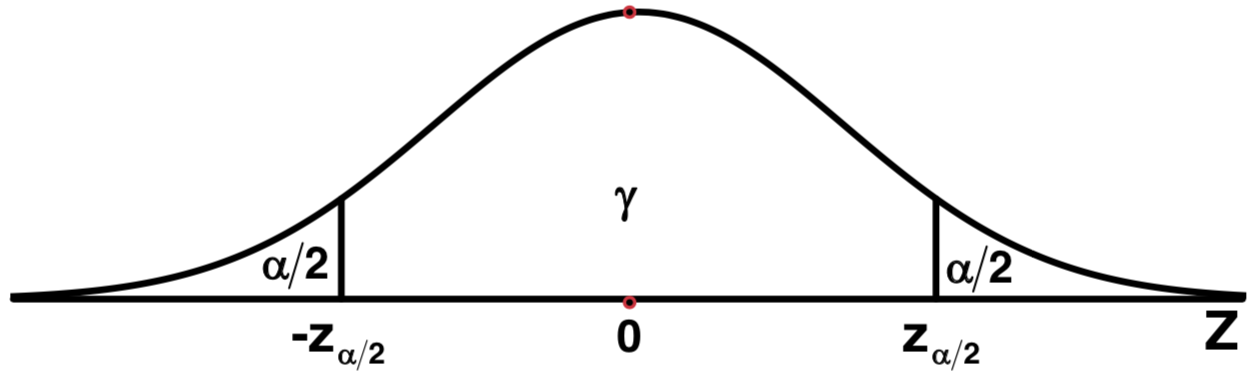
\includegraphics[width=6.5cm]{Graficos/fig1_CE}		}{  \caption*{}	}
	%
\end{floatrow}
\end{figure}
	
	\vspace{-3\baselineskip}
	%
	Cuando no se especifica el valor de \(\gamma\) y no se pide calcularlo, se supone que su valor es igual a \(0,95\).
\end{observ}


\begin{proposicion}
	Intervalo de confianza para la media \(\mu=\Esp[X]\), conocida \(\sigma^2=\Var[X]\); \(\bar{x}-B<\mu\bar{x}+B\), donde \(B=z_{\nicefrac{\alpha}{2}}\sqrt{\Var[\bar{X}]}\) y \(\Var[\bar{X}]=\dfrac{\sigma^2}{n}\).
\end{proposicion}
\begin{proof}
	Por el Teorema del Límite Central, si \(X\sim\Normal(\mu,\sigma^2)\) o \(n\) es suficientemente grande, \(\bar{X}\sim\Normal\left(\mu,\dfrac{\sigma^2}{n}\right)\), por lo que \(\Var[\bar{X}]=\dfrac{\sigma^2}{n}\), entonces \(Z=\nicefrac{\bar{X}-\mu}{\sigma}\sqrt{n}\) y \(P(-z_{\nicefrac{\alpha}{2}}<Z<z_{\nicefrac{\alpha}{2}})=\gamma\), lo cual es lo mismo que \(P\left(-z_{\nicefrac{\alpha}{2}}<\dfrac{\bar{X}-\mu}{\sigma}\sqrt{n}<z_{\nicefrac{\alpha}{2}}\right)=\gamma\), de donde \(P\left(\bar{X}-z_{\nicefrac{\alpha}{2}}\dfrac{\sigma}{\sqrt{n}}<\mu<\bar{X}+z_{\nicefrac{\alpha}{2}}\dfrac{\sigma}{\sqrt{n}}\right)=\gamma\). Por este resultado y utilizando la observación \eqref{obs-4.2}; \(B=z_{\nicefrac{\alpha}{2}}\dfrac{\sigma}{\sqrt{n}}\).  Como \(\Var[\bar{X}]=\dfrac{\sigma^2}{n}\), \(B\) se puede escribir como \(B=z_{\nicefrac{\alpha}{2}}\sqrt{\Var[\bar{X}]}\).
\end{proof}

\begin{observ}\label{obs-4.4}
	Por el resultado obtenido para \(B\): \(B=z_{\nicefrac{\alpha}{2}}\dfrac{\sigma}{\sqrt{n}}\)
	\begin{APAenumerate}
		\item \(B\) y \(n\) son inversamente proporcionales; por lo tanto, si se resuelve disminuir el límite para el error de estimación \(B\),  se debe incrementar el tamaño de la muestra \(n\).
		\item \(n=\dfrac{z_{\nicefrac{\alpha}{2}}^2\sigma^2}{B^2}\), por lo que \(z_{\nicefrac{\alpha}{2}}\) y \(n\) son directamente proporcionales. Si se resuelve aumentar el nivel de confianza \(\gamma\), se debe aumentar	 el valor de \(z_{\nicefrac{\alpha}{2}}\) con lo cual \(\gamma\) y \(n\) son directamente proporcionales; es decir, si se resuelve incrementar el valor de \(\gamma\), se debe incrementar el tamaño de la muestra.
	\end{APAenumerate}

Como para todo intervalo de confianza se aspira que sea pequeño el límite para el error de estimación y el nivel de confianza lo más grande posible, por los análisis realizados, el tamaño de la muestra debe ser suficientemente grande; lo que se opone a otras variables que intervienen en los procesos de muestreo tales como: costos, tiempo, recursos humanos, etc.

Por lo anterior, en la mayoría de estudios referentes a muestreo, uno de los aspectos fundamentales es el cálculo del tamaño de la muestra, para lo que se consideran a más del límite para el error de estimación y el nivel de confianza, otras variables como las mencionadas que no siempre es posible cuantificarlas
de manera más o menos precisa.
\end{observ}



%
%%%
%%%%% 	
%%%%%%%
\subsubsection{Muestreo aleatorio simple}

\neodefi{Sin considerar el tamaño de la población}

\neodefi{Para la media} 

Para estimar la media de una variable cuantitativa en una población a través de intervalos de confianza, existen dos posibilidades como consecuencia de la medida de variabilidad que se conozca:

\vspace{0.75\baselineskip}
	\textbf{Si se conoce la varianza \(\sigma^2\) (o la desviación estándar \(\sigma\)) de la variable en la población en estudio}\newline


Se utiliza lo desarrollado en la proposición \eqref{prop-4.2} \(\), \(\bar{x}-B<\mu<\bar{x}+B\), donde \(Bz_{\nicefrac{\alpha}{2}} 	\sqrt{\Var[\bar{X}]}\), \(\Var[\bar{X}]=\dfrac{\sigma^2}{n}\).

\begin{ejem}
	Un psicólogo desea estimar el tiempo medio de reacción de sus pacientes, para un estímulo especial, suponiendo que la desviación estándar de ese tiempo es igual a \(0.8\) segundos.
	\begin{APAenumerate}
		\item Con una muestra aleatoria de 73 pacientes obtuvo un promedio de \(4.1\) segundos. Calcule el intervalo de confianza para la media, al \(93\%\).
		\item Calcule el tamaño mínimo de la muestra para estimar la media poblacional si la longitud del intervalo de confianza es igual a \(0.32\) segundos y el nivel de confianza igual a \(0.96\).
	\end{APAenumerate}
\end{ejem}

\begin{proof}[Solución]\quad
	\begin{enumerate}
		\item \(n=73\); \(\bar{x}=42\); \(\sigma=0.8\); \(\gamma=0.93\)
		
		\(\bar{x}-B<\mu<\bar{x}+B\); \(B=z_{\nicefrac{\alpha}{2}}\sqrt{\Var[\bar{X}]}\); \(\Var[\bar{X}]=\dfrac{\sigma^2}{n}\); \(B=z_{\nicefrac{\alpha}{2}}\sqrt{\dfrac{\sigma^2}{n}}\); \(P(Z<z_{\nicefrac{\alpha}{2}})=0.965\); \(z_{\nicefrac{\alpha}{2}}=1.81\)
		
		\(B=1.81\sqrt{\dfrac{0.8^2}{73}}=1.69\); \(4.1-0.169<\mu<4.1+0.169\); \(3.931<\mu<4.269\)
		
		\vspace{1\baselineskip}
		\item \(\sigma=0.8\); \(L=0.32\); \(\gamma=0.96\)
		
		Para calcular el tamaño de la muestra: \(B=z_{\nicefrac{\alpha}{2}}\sqrt{\dfrac{\sigma^2}{n}}\), de donde \(n=\dfrac{z_{\nicefrac{\alpha}{2}}^2\sigma^2}{B^2}\)
		
		\(B=\dfrac{L}{2}=\dfrac{0.32}{2}=0.16\); \(P(Z<z_{\nicefrac{\alpha}{2}})=0.98\);
		
		\(z_{\nicefrac{\alpha}{2}}=2.05\); \(n=\dfrac{2.05^2 \times 0.8^2}{0.16^2}=105.0625\)
		
		El tamaño de toda muestra \(n\) es un número entero y \(B\) se define como el límite para el error de estimación, por lo que el resultado obtenido para \(n\) debe aproximarse.
		
		Si \(n=105\), \(B=z_{\nicefrac{\alpha}{2}}\sqrt{\dfrac{\sigma^2}{n}}=2.05\sqrt{\dfrac{0.8^2}{105}}=1.160047\)
		
		Si \(n=106\), \(B=z_{\nicefrac{\alpha}{2}}\sqrt{\dfrac{\sigma^2}{n}}=2.05\sqrt{\dfrac{0.8^2}{106}}=0.15929\)
		
		Por lo tanto, el tamaño mínimo de la muestra es igual a \(106\).			\qedhere
	\end{enumerate}
\end{proof}



\vspace{0.75\baselineskip}
	\textbf{Si se conoce la varianza \(s^2\) (o la desviación estándar \(s\)) de una muestra de la población en estudio (no se conoce \(\sigma^2\)).}\newline

\begin{proposicion}\label{prop-5.1}
	La variable \(T=\dfrac{\bar{X}-\mu}{S}\sqrt{n}\) tiene una distribución \(t\) de student con \(n-1\) grados de libertad.
\end{proposicion}


\begin{proposicion}\label{prop-5.2}
	El intervalo de confianza para la media \(\mu\) está dado por \(\bar{x}-B<\mu<\bar{x}+B\), con \(B=t_{\nicefrac{\alpha}{2},n-1} \sqrt{\Var[\bar{X}]}\); \(\Var[\bar{X}]=\dfrac{s^2}{n}\).
\end{proposicion}
\begin{proof}
	\(\bar{X}\) es estimador insesgado de \(\mu\), entonces \(P(\bar{X}-B<\mu<\bar{X}+B)=\gamma\) y el intervalo de confianza es igual a \(\bar{x}-B<\mu<\bar{x}+B\).
	
	Por la proposición \eqref{prop-5.1} y el comportamiento de la distribución \(t\) de student 
	\[
		P(-t_{\nicefrac{\alpha}{2},n-1}<T<t_{\nicefrac{\alpha}{2},n-1})= P\left(-t_{\nicefrac{\alpha}{2},n-1}<\dfrac{\bar{X}-\mu}{s}<t_{\nicefrac{\alpha}{2},n-1}\right)=\gamma,
	\]
	de donde  
	\[
		P\left(\bar{X}-t_{\nicefrac{\alpha}{2},n-1}\dfrac{s}{\sqrt{n}}<\mu<\bar{X}+t_{\nicefrac{\alpha}{2},n-1}\dfrac{s}{\sqrt{n}}\right)=\gamma. 
	\]	
	Por lo tanto: \(B=t_{\nicefrac{\alpha}{2},n-1}\dfrac{s}{\sqrt{n}}\).
	
	\(s^2\) estima a \(\sigma^2\), \(\Var[\bar{X}]=\dfrac{s^2}{n}\) estima a \(\Var[\bar{X}]=\dfrac{\sigma^2}{n}\), con lo cual \(B=t_{\nicefrac{\alpha}{2},n-1}\sqrt{\Var[\bar{X}]}\); \(\Var[\bar{X}]=\dfrac{s^2}{n}\).
\end{proof}


\begin{observ}\quad
	\begin{APAenumerate}
		\item Los valores de la distribución \(t\) de student son similares a los de la distribución normal estándar, cuando \(n\) toma valores altos.
		\item Para calcular \(t_{\nicefrac{\alpha}{2},n-1}\), se utiliza la relación \(P(T>t_{\nicefrac{\alpha}{2},n-1})=\dfrac{\alpha}{2}\), con \(\gamma+\alpha=1\).
	\end{APAenumerate}
\end{observ}


\begin{ejem}
	En un estudio de mercado sobre la cantidad mensual utilizada para adquirir productos de aseo personal.
	\begin{enumerate}
		\item Se tomó una muestra de 54 familias, obteniéndose que en promedio utilizaban \(67.2\) dólares mensuales y la desviación estándar era igual a \(39.5\) dólares. Calcule el intervalo de confianza para la cantidad mensual media familiar empleada en productos de aseo personal, al \(90\%\).
		\item Calcule el tamaño mínimo muestral necesario para calcular el intervalo de confianza para la cantidad mensual media que utiliza la población en estudio para adquirir productos de aseo, si el límite para el error de estimación es igual a \(7.9\) dólares y el nivel de confianza es igual a \(0.94\).
	\end{enumerate}
\end{ejem}
\begin{proof}[Solución]\quad
	\begin{APAenumerate}
		\item \(n=54\); \(\bar{x}=62.7\); \(s=39.5\), \(\gamma=0.9\)
		
		\(\bar{x}-B<\mu<\bar{x}+B\); \(B=t_{\nicefrac{\alpha}{2},n-1}\sqrt{\Var[\bar{X}]}\); \(\Var[\bar{X}]=\dfrac{s^2}{n}\), entonces \(B=t_{\nicefrac{\alpha}{2},n-1}\sqrt{\dfrac{s^2}{n}}\)
		
		\(P(T_{53}>t_{\nicefrac{\alpha}{2},n-1})=0.05\); \(t_{\nicefrac{\alpha}{2},n-1}=1.673\) (aproximadamente \(53\) a \(55\) y utilizando la tabla 2 de este documento)
		
		\(B=1.673\sqrt{\dfrac{39.5^2}{54}}=8.842\), entonces \(67.2-8.842<\mu<67.2+8.842\); \(58.358<\mu<76.042\) 
		
		\vspace{1\baselineskip}
		\item \(s=39.5\); \(B=7.9\); \(\gamma=0.94\)
		
		De \(B=t_{\nicefrac{\alpha}{2},n-1}\sqrt{\dfrac{s^2}{n}}\); \(n=\dfrac{t_{\nicefrac{\alpha}{2},n-1}^2s^2}{B^2}\).
		
		Como no se conoce el valor de \(n\) (lo que se solicita), no es posible obtener \(t_{\nicefrac{\alpha}{2},n-1}\), por lo que aproximamos su valor con el de \(z_{\nicefrac{\alpha}{2}}\); \(P(Z<z_{\nicefrac{\alpha}{2}})=0.97\); \(z_{\nicefrac{\alpha}{2}}=1.88\)
		
		\(n=\dfrac{1.88^2*39.5^2}{7.9^2}=88.26\); \(n =89\)
		
		Para calcular \(n\) se utilizó la distribución normal en lugar de  la distribución de student, por lo que es necesario realizar un ajuste, comenzando con el valor calculado para \(n\), hasta obtener el mínimo valor que garantice que el valor de \(B\) no supere al determinado (\(7.9\)).
		
		Ajuste
		\[
		P(T_{n-1}>t_{\nicefrac{\alpha}{2},n-1})=0.03
		\]
		\vspace{-1\baselineskip}
		
	\begin{table}[H]
	\fontsize{7.25}{11}\selectfont
	\centering
	\begin{tabular}{l  c cc cc} \thickline
		\(n\) & \(n-1\) 	&	\(t_{\nicefrac{\alpha}{2},n-1}\)	&  \(B=t_{\nicefrac{\alpha}{2},n-1}\sqrt{\dfrac{s^2}{n}}\) 
		\vspace{0.5em}
	 		\\     \hline
		89    & 88(90)  	& 1.9048                           & \(B=1.9048\sqrt{\dfrac{38.9^2}{89}}\approx 7.975\)             \\
		90    & 89(90)  	& 1.9048                           & \(B=1.9048\sqrt{\dfrac{39.5^2}{90}}\approx 7.931\)             \\
		91    & 90      	& 1.9048                           & \(B=1.9048\sqrt{\dfrac{39.5^2}{91}}\approx 7.887\)                                                                          
	\end{tabular}
	\end{table}
		
	El tamaño mínimo de la muestra es \(91\).			\qedhere
	\end{APAenumerate}
\end{proof}



\neodefi{Para la proporción}

Para la proporción, \(X\): <<Número de éxitos en los \(n\) procesos de Bernoulli>>, donde \(P(E)=p\) y \(P(F)=q=1-p\) constantes para los \(n\) procesos \(X_1,X_2,\ldots,X_n\) aleatorios e independientes, con 
\[
	X_i=\begin{cases} 1 & E,\\ 0 & F;\end{cases}
	\qquad
	P(X_i=1)=P(E)=p;
	\qquad
	P(X_i=0)=P(F)=q;
\]
y \(\Esp[X_i]=p\), \(\Var[X_i]=pq\), para todo \(i \in \{1,\ldots,n\}\); con lo cual se puede escribir: \( X=\displaystyle\sum_{i=1}^{n}X_i\), entonces \(P=\dfrac{X}{n}=\dfrac{1}{n}\dsum_{i=1}^{n}X_i=\bar{X}\).

\begin{proposicion}
	El intervalo de confianza para la proporción \(p\), conocida \(p\) está dado por \(\hat{p}-B<p<\hat{p}+B\), donde: \(B=z_{\nicefrac{\alpha}{2}}\sqrt{\Var[\hat{p}]}\); \(\Var[\hat{p}]=\dfrac{pq}{n}\).
\end{proposicion}
\begin{proof}
	Por la proposición \eqref{prop-4.1}, \(P=\dfrac{X}{n}=\dfrac{1}{n}\displaystyle\sum_{i=1}^{n}X_i=\bar{X}\) es un estimador insesgado de \(p\). Por la definición \eqref{def-4.4} \(P\big(\left|\hat{P}-p\right|<B\big)=\gamma\), lo que es equivalente a  \(P(\hat{P}-B<p<\hat{P}-p)=\gamma\) y el intervalo de confianza para  \(p\) es \(\hat{p}-B<p<\hat{p}+B\).
	
	Como \(P=\bar{X}\), utilizando el Teorema del Límite Central, \(P=\bar{X}\sim\Normal\big(\Esp[\hat{P}],\Var[\hat{P}]\big)\) asintóticamente (\(n\) suficientemente grande).
	
	Por los resultados obtenidos en la proposición \eqref{prop-4.1} \(\Esp[\hat{P}]=p\) y \(\Var[\hat{P}]=\dfrac{pq}{n}\); por lo tanto, \(P\sim\Normal\left(p,\dfrac{pq}{n}\right)\). Entonces \(Z=\dfrac{\bar{X}-\mu}{\sigma}\sqrt{n}\) y \(P(-z_{\nicefrac{\alpha}{2}}<Z<z_{\nicefrac{\alpha}{2}})=\gamma\)
	
	\begin{figure}[H]
\hspace{-3.5em}
\begin{floatrow}
	\fontsize{8}{11}\selectfont
	\captionsetup{justification=centering, labelfont=footnotesize, font=footnotesize}
	%	Tabla
	\capbtabbox{%
	$
	P( Z<z_{\nicefrac{\alpha}{2}} )=
	\begin{cases}
		1-\nicefrac{\alpha}{2} \\
		\nicefrac{\alpha}{2}+\gamma \vspace{2.5\baselineskip} \\
		\dfrac{1+\gamma}{2}
	\end{cases}
	$
	\vspace{2.1em}
	}{	  \caption*{}%
	}
	%	Figura
	\ffigbox{	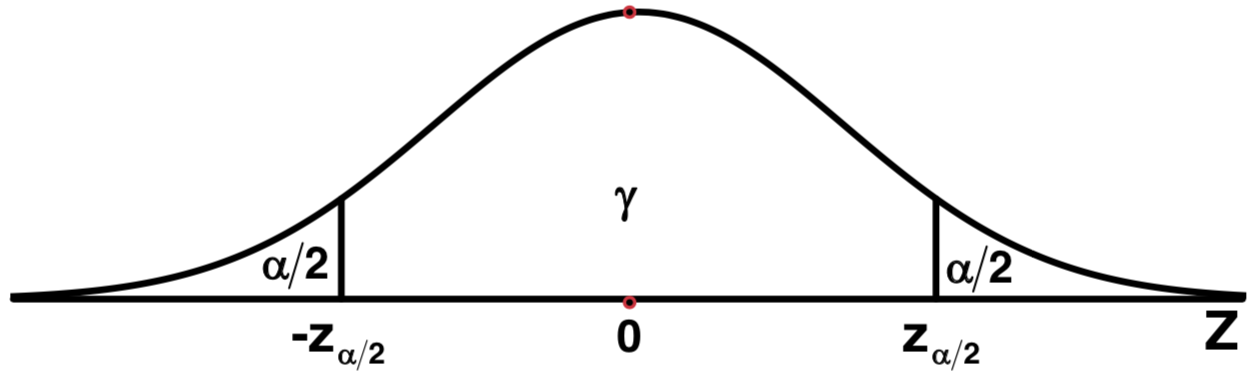
\includegraphics[width=6.5cm]{Graficos/fig1_CE}		}{  \caption*{}	}
	%
\end{floatrow}
\end{figure}
	
	\vspace{-3\baselineskip}
	\(P\left(-z_{\nicefrac{\alpha}{2}}<\dfrac{\bar{X}-p}{pq}\sqrt{n}<z_{\nicefrac{\alpha}{2}}\right)=\gamma\), de donde \(P\left(\bar{X}-z_{\nicefrac{\alpha}{2}}\dfrac{p1}{\sqrt{n}}<p<\bar{X}+z_{\nicefrac{\alpha}{2}}\dfrac{pq}{\sqrt{n}}\right)=\gamma\), con lo cual \(B=z_{\nicefrac{\alpha}{2}}\dfrac{pq}{n}\) y como \(\Var[\hat{P}]=\dfrac{pq}{n}\), \(B\) se puede escribir como \(B=z_{\nicefrac{\alpha}{2}}\dfrac{pq}{\sqrt{n}}\).
\end{proof}

\begin{ejem}
	El auditor de una empresa está interesado en conocer la proporción de comprobantes que podrían 	estar archivados incorrectamente. Se sabe que en empresas similares, el \(8\%\) de los comprobantes se archivan incorrectamente
	\begin{APAenumerate}
		\item Calcule el intervalo de confianza para la proporción de comprobantes que podrían estar mal archivados, si se toma una muestra de tamaño \(172\).
		\item Si se fija la longitud del intervalo de confianza en \(0.066\) y el nivel de confianza en \(0.93\), calcule el tamaño de muestra mínimo necesario para hacer el estudio.
	\end{APAenumerate}
\end{ejem}
\begin{proof}[Solución]\quad
	\begin{APAenumerate}
		\item \(p=0.08\); \(n=172\); \(\gamma=0.95\)
		
		\(B=z_{\nicefrac{\alpha}{2}}\sqrt{\Var[\hat{P}]}\), donde \(\Var[\hat{P}]=\dfrac{pq}{n}\); \(B=z_{\nicefrac{\alpha}{2}}\sqrt{\dfrac{pq}{n}}\); \(P(Z<z_{\nicefrac{\alpha}{2}})=0.975\); \(z_{\nicefrac{\alpha}{2}}=1.96\).
		
		Entonces  \(B=1.96\sqrt{\dfrac{0.08 \times 0.92}{172}}=0.0405\).
		
		Como se conoce el valor de \(p\), el intervalo de confianza es igual a 
		\[0.08-0.0405<p<0.08+0.0405 ; \qquad 0.0395<p<0.1205.\]
		
		\vspace{1\baselineskip}
		\item \(p=0.08\); \(\gamma=0.93\); \(L=0.066\); \(B=0.033\); \(P(Z<z_{\nicefrac{\alpha}{2}})=0.965\); \(z_{\nicefrac{\alpha}{2}}=1.81\)
		
		\(B=z_{\nicefrac{\alpha}{2}}\sqrt{\dfrac{pq}{n}}\), de donde \(n=\dfrac{z_{\nicefrac{\alpha}{2}}^2*pq}{B^2}\); \(n=\dfrac{1.81^2 \times 0.08 \times 0.92}{0.033^2}=221.415\). El tamaño mínimo de la muestra es \(222\).		\qedhere
	\end{APAenumerate}
\end{proof}


\begin{proposicion}\label{prop-5.4}
	El intervalo de confianza para la proporción \(p\), conocida \(\hat{p}\) está dado por \(\hat{p}-B<p<\hat{p}+B\), donde \(B=z_{\nicefrac{\alpha}{2}}\sqrt{\Var[\hat{P}]}\); \(\Var[\hat{P}]=\dfrac{pq}{n}\).
\end{proposicion}
\begin{proof}
	Por la proposición \eqref{prop-4.1}, \(P=\dfrac{X}{n}=\dfrac{1}{n}\displaystyle\sum_{i=1}^{n}X_i=\bar{X}\) es un estimador insesgado de \(p\). Por lo tanto \(P(\hat{P}-B<p<\hat{P}-B)=\gamma\) y el intervalo de confianza para \(p\) es \(\hat{p}-B<p<\hat{p}+B\).
	
	\(\hat{p}\) estima a \(p\); \(\Var[\hat{P}]\dfrac{pq}{n}\) estima a \(\Var[P]=\dfrac{pq}{n}\), con lo cual por lo tanto \(\hat{p}-B<p<\hat{p}+B\) es el intervalo de confianza para \(p\), con \(B=z_{\nicefrac{\alpha}{2}}\sqrt{\Var[\hat{P}]}\); \(\Var[\hat{P}]=\dfrac{pq}{n}\).
\end{proof}


\begin{observ}
	Si nada se conoce como \(p\), se considera a \(p=q=0.5\), ya que, como primera aproximación, con esos valores se obtiene el mayor valor posible para \(B=z_{\nicefrac{\alpha}{2}}\sqrt{\dfrac{pq}{n}}\).
\end{observ}

\begin{ejem}
	Con una muestra piloto de \(764\) votantes respecto a que la Asamblea Nacional elija a los miembros de la Corte Suprema de Justicia, el \(20\%\) respondió estar de acuerdo.
	\begin{APAenumerate}
		\item Calcule el intervalo de confianza al \(95\%\) para la proporción de votantes que están de acuerdo con ese planteamiento.
		\item Se ha resuelto que se realice el estudio definitivo con el límite para el error de estimación igual a \(0.02\) y el nivel de confianza igual a \(0.97\). Calcule el tamaño mínimo de muestra para realizar el estudio.
	\end{APAenumerate}
\end{ejem}
\begin{proof}[Solución]\quad
	\begin{APAenumerate}
		\item \(n=764\); \(p=0.2\); \(\gamma=0.95\); \(P(Z<z_{\nicefrac{\alpha}{2}})=0.975\); \(z_{\nicefrac{\alpha}{2}}=1.96\)
		
		\(\hat{p}-B<p<\hat{p}+B\), \(B=z_{\nicefrac{\alpha}{2}}\sqrt{\Var[\hat{P}]}\); \(\Var[\hat{P}]=\dfrac{pq}{n}\); \(B=z_{\nicefrac{\alpha}{2}}\sqrt{\dfrac{pq}{n}}\), entonces 
		
		\(B=1.96\sqrt{\dfrac{0.2 \times 0.8}{764}}=0.0283641\); \(0.1-0.0283541<p<0.2+0.0283641\); \(0.1716359<p<0.02283641\).
		
		\vspace{1\baselineskip}
		\item \(B=0.025\); \(p=0.2\); \(\gamma=0.96\); \(P(Z<z_{\nicefrac{\alpha}{2}})=0.98\); \(z_{\nicefrac{\alpha}{2}}=2.05\); \(B=z_{\nicefrac{\alpha}{2}}\sqrt{\dfrac{\hat{p}{\hat{q}}}{n}}\); \(n=\dfrac{z_{\nicefrac{\alpha}{2}}^2\hat{p}\hat{q}}{B^2}\)
		\(n=\dfrac{2.05^2 \times 0.2 \times 0.8}{0.025^2}=1075.84\); \(n=1076\).		\qedhere
	\end{APAenumerate}
\end{proof}

%
%
%
\newpage
\neodefi{Muestreo aleatorio simple considerando el tamaño de la población}


\begin{proposicion}
	Supóngase una población de \(N\) elementos que tienen igual probabilidad de ser incluidos en cualquier muestra extraída al azar; \(y_1.y_2.\ldots,y_n\) representan los valores asignables a cada uno de los elementos de la población al aplicársele una variable aleatoria \(X\); \(\Esp[X]=\mu\); \(\Var[X]=\sigma^2\); \(X_1.X_2.\ldots,X_n\)una muestra de variables aleatorias idénticamente distribuidas (que se obtienen al aplicar \(n\) veces \(X\) en la población) con \(\Esp[X_i]=\mu\); \(\Var[X_i]=\sigma^2\); \(\bar{X}=\dfrac{1}{n}\displaystyle\sum_{i=1}^{n}X_i\); \(S^2=\dfrac{1}{n-1}\displaystyle\sum_{i=1}^{n}(X_i-\bar{X})^2\). Entonces:
	\begin{APAenumerate}
		\item \(\Esp[\bar{X}]=\Esp[X]=\mu\) (\(\bar{X}\) es un estimador insesgado de \(\Esp[X]\)),
		\item \(\cov(X_i,X_j)=-\dfrac{\sigma^2}{N-1}\),
		\item \(\Var[\bar{X}]=\dfrac{s^2}{n}\left(\dfrac{N-n}{N-1}\right)\),
		\item \(\Esp[S^2]=\dfrac{\sigma^2N}{N-1}\),
		\item Si \(\Var[\bar{X}]=\dfrac{s^2}{n}\left(\dfrac{N-n}{N}\right)\), entonces  \(\Esp\big[\Var[\bar{X}]\big]=\Var[\bar{X}]\)
		(\(\Var[\bar{X}]\) es un estimador insesgado de \(\Var[X]\)).
	\end{APAenumerate}
\end{proposicion}


\neodefi{Para la media} 

El intervalo de confianza para la media: \(\bar{x}-B<\mu<\bar{x}+B\).

\vspace{0.75\baselineskip}
	\textbf{Si se conoce la varianza \(\sigma^2\)(o la desviación estándar \(\sigma\)) de la variable en la población en estudio}
	\[
		B=z_{\nicefrac{\alpha}{2}}\sqrt{\Var[\bar{X}]}, \qquad \Var[\bar{X}]=\dfrac{\sigma^2}{n}\left(\dfrac{N-n}{N-1}\right)
	\]
	

\begin{ejem}
	En la fabricación de \(1462\) soportes de caucho se ha resuelto trabajar con las siguientes condiciones: el intervalo de confianza para la media de dureza igual a \([158 ; 165] \) la varianza del proceso igual a \(169\); el nivel de confianza del intervalo igual a \(0.92\). Calcule el tamaño mínimo de la muestra que cumple con las condiciones planteadas.
\end{ejem}
\begin{proof}[Solución]\qquad

		\(N=1462\); \([158;165]\); \(\sigma^2=169\); \(\gamma=0.92\); \(P(Z<z_{\nicefrac{\alpha}{2}})=0.96\); \(z_{\nicefrac{\alpha}{2}}=1.75\)
		
		\(B=z_{\nicefrac{\alpha}{2}}\sqrt{\Var[\bar{X}]}\); \(\Var[\bar{X}]=\dfrac{\sigma^2}{n}\left(\dfrac{N-n}{N-1}\right)\); \(B=z_{\nicefrac{\alpha}{2}}\sqrt{\dfrac{\sigma^2(N-n)}{n(N-1)}}\)
		
		\(n=\dfrac{z_{\nicefrac{\alpha}{2}}^2\sigma^2 N}{B^2(N-1)+z_{\nicefrac{\alpha}{2}}^2\sigma^2}=\dfrac{1.75^2 \times 169 \times 1462}{3.5^2 \times 1461+1.75^2 \times 169}=41.0906\ldots\); \(n=42\)
\end{proof}


\vspace{0.75\baselineskip}
	\textbf{Si se conoce la varianza \(s^2\) (o la desviación estándar \(s\)) de una muestra de la población en estudio (no se conoce \(\sigma^2\)) }
	\[
		B=t_{\nicefrac{\alpha}{2},n-1}\sqrt{\Var[\bar{X}]}; \qquad
		\Var[\bar{X}]=\dfrac{s^2}{n}\left(\dfrac{N-n}{N}\right)
	\]
	

\begin{ejem}
	Para producir \(587\) piezas se ha resuelto realizar una prueba con \(16\), respecto al peso (en gramos). La muestra piloto obtenida es:
	\[\begin{Bmatrix}
	97.9 & 88.0 & 94.6 & 97.0 & 98.1 & 80.1 & 79.9 & 87.1 \\
	 88.0 & 93.4 & 84.4 & 79.0 & 87.9 & 80.6 & 94.2 & 86.0
	\end{Bmatrix}\]

\begin{APAenumerate}
	\item Calcule el intervalo de confianza para la media de producción al \(93\%\). 
	\item Para el estudio muestral definitivo se ha resuelto fijar el límite para el error de estimación igual a \(2.4\) gramos y el nivel de confianza igual a \(0.96\). Calcule el tamaño mínimo de muestra que cumpla lo establecido.
\end{APAenumerate}
\end{ejem}
\begin{proof}[Solución]\quad
	\begin{APAenumerate}
		\item \(N=587\); \(n=16\); \(\gamma=0.93\); \(\bar{x}=88.5125\); \(s=6.681\ldots\); \(P(T_{15}>t_{\nicefrac{\alpha}{2},n-1})=0.035\); \(t_{\nicefrac{\alpha}{2},n-1}=1.9509\)
		
		\(\bar{x}-B<\mu<\bar{x}+B\); \(B=t_{\nicefrac{\alpha}{2},n-1}\sqrt{\Var[\bar{X}]}\); \(\Var[\bar{X}]=\dfrac{s^2}{n}\left(\dfrac{N-n}{N}\right)\);
		
		\(B=t_{\nicefrac{\alpha}{2},n-1}\sqrt{\dfrac{s^2(N-n)}{Nn}}=1.9509\sqrt{\dfrac{{6.681\ldots}^2(587-1)}{16 \times 587}}=3.21377\ldots\)
		
		\(88.5125-3.21377\ldots<\mu<88.5125+3.21377\ldots\); \(85.2987\ldots<\mu<91.72627\ldots\)
		
		\vspace{1\baselineskip}
		\item \(N=5887\); \(B=2.6\); \(\gamma=0.96\); \(s=6.681005...\);
		 
		\(B=t_{\nicefrac{\alpha}{2},n-1}\sqrt{\dfrac{s^2(N-n)}{Nn}}\); \(n=\dfrac{t_{\nicefrac{\alpha}{2},n-1}^2s^2N}{B^2N+t_{\nicefrac{\alpha}{2},n-1}^2s^2}\);
		
		Como no se conoce el valor de \(n\) (lo que se solicita), no es posible obtener \(t_{\nicefrac{\alpha}{2},n-1}\), por lo que 	aproximamos su valor con el de \(z_{\nicefrac{\alpha}{2}}\); \(P(Z<z_{\nicefrac{\alpha}{2}})=0.98\); \(z_{\nicefrac{\alpha}{2}}=2.05\)
		\(n=\dfrac{2.05^2 \times 6.681\ldots^2 \times 587}{2.6^2 \times 587+2.05^2 \times 6.681\ldots^2}=26.49\ldots\); \(n=27\)
		
		Para calcular \(n\) se utilizó la distribución normal en lugar de la distribución de student, por lo que es necesario realizar un ajuste, comenzando con el valor calculado para n, hasta obtener el mínimo valor que garantice que el valor de \(B\) no supere al determinado (\(2.6\)).
		
		Ajuste \[P(T_{n-1}>t_{\nicefrac{\alpha}{2},n-1})=0.02\]
		
		
	\vspace{-1\baselineskip}	
	\begin{table}[H]
	\fontsize{7.25}{11}\selectfont
	\centering
	\begin{tabular}{l  c cc cc} \thickline
		\(n\) & \(n-1\) 	&	\(t_{\nicefrac{\alpha}{2},n-1}\)	&  \(B=t_{\nicefrac{\alpha}{2},n-1}\sqrt{\dfrac{s^2(N-n)}{nN}} \) 
		\vspace{0.5em}
	 		\\     \hline
		27    & 26      & 2.162                            & 2.7151\ldots                                                  \\
		28    & 27      & 2.1578                           & 2.6586\ldots                                                  \\
		29    & 28      & 2.1539                           & 2.6053\ldots                                                  \\
		30    & 29      & 2.1503                           & 2.5549\ldots  
	\end{tabular}
	\end{table}

	
	El tamaño mínimo de la muestra es \(30\).				\qedhere
	\end{APAenumerate}
\end{proof}


\newpage

\neodefi{Para el total}

\begin{proposicion}\label{prop-5.6}\quad
	\begin{APAenumerate}
		\item \(\hat{T}=N\hat{X}\) es un estimador insesgado para el total \(T=N\mu\)
		\item Si se conoce la varianza \(\sigma^2\)(o la desviación estándar \(\sigma\)) de la variable en la población en estudio, el intervalo de confianza para el total está dado por \(\hat{t}-B<T<\hat{t}+B\), donde \(\hat{t}=N\bar{x}\); \(B=z_{\nicefrac{\alpha}{2}}\sqrt{\Var[\bar{T}]}\); \(\Var[\hat{T}]=N^2\Var[\bar{X}]\).
		\item Si se conoce la varianza \(s^2\) (o la desviación estándar \(s\)) de una muestra de la población en estudio (no se conoce \(\sigma^2\)), el intervalo de confianza total está dado por \(\hat{t}-B<T<\hat{t}+B\), donde \(\hat{t}=N\bar{x}\); \(B=t_{\nicefrac{\alpha}{2},n-1}\sqrt{\Var[\hat{T}]}\); \(\hat{\Var}[\hat{T}]=N^2\Var[\bar{X}]\).
	\end{APAenumerate}
\end{proposicion}
\begin{proof}\quad
	\begin{APAenumerate}
		\item El total \(T\) está dado por \(T=N\mu\). Como \(\bar{X}\) es un estimador insesgado de \(\mu\), \(\hat{T}=N\bar{x}\) es un estimador insesgado de \(T\), ya que \(\Esp[\hat{T}]=\Esp[N\bar{X}]=N\Esp[\bar{X}]=N\mu=T\).
		
		\vspace{1\baselineskip}
		\item El intervalo de confianza para \(\mu\) está dado por: \(\bar{x}-B<\mu<\bar{x}+B\); con \(B=z_{\nicefrac{\alpha}{2}}\sqrt{\Var[\bar{X}]}\)
		
		\(N\bar{x}-BN<N\mu<N\bar{x}+NB\); \(\hat{t}=N\bar{x}\); \(T=N\mu\)
		
		\(NB=Nz_{\nicefrac{\alpha}{2}}\sqrt{\Var[\bar{X}]}=z_{\nicefrac{\alpha}{2}}\sqrt{N^2\Var[\bar{X}]}=z_{\nicefrac{\alpha}{2}}\sqrt{\Var[\hat{T}]}\); luego \(\hat{t}-B<T<\hat{t}+B\) con \(B=z_{\nicefrac{\alpha}{2}}\sqrt{\Var[\hat{T}]}\); \(\Var[\hat{T}]=N^2\Var[\bar{X}]\).
		
		\vspace{1\baselineskip}
		\item El intervalo de confianza para \(\mu\) está dado por: \(\bar{x}-B<\mu<\bar{x}+B\); con \(B=t_{\nicefrac{\alpha}{2},n-1}\sqrt{\Var[\bar{X}]}\);
		
		\(N\bar{x}-NB<N\mu<N\bar{x}+NB\); \(\hat{t}=N\bar{x}\); \(T=N\mu\)
		
		\(NB=Nt_{\nicefrac{\alpha}{2},n-1}\sqrt{\Var[\bar{X}]}=t_{\nicefrac{\alpha}{2},n-1}\sqrt{N^2\Var[\bar{X}]}=t_{\nicefrac{\alpha}{2},n-1}\sqrt{\Var[\hat{T}]}\); luego \(\hat{t}-B<T<\hat{t}+B\), con \(B=t_{\nicefrac{\alpha}{2},n-1}\sqrt{\Var\hat{T}}\).									\qedhere
	\end{APAenumerate}
\end{proof}


\begin{ejem}\label{ejem-5.7}
	En el supermercado se está realizando un estudio sobre los ingresos anuales.
	\begin{APAenumerate}
		\item Con la muestra aleatoria piloto de los ingresos diarios (en miles de dólares) obtenida, calcule el intervalo de confianza para el total de los 365 días del año.
		\[\setcounter{MaxMatrixCols}{20}
		\begin{Bmatrix}
	4.66 & 3.85 & 3.97 & 5.02 & 4.14 & 4.24 & 3.42 & 4.22& 3.63 & 4.99  \\
	5.57 & 4.70 & 5.44 & 4.70 & 5.02 & 4.38 & 4.63 & 5.18 & 3.81 & 4.53 \\
	4.84 & 4.58 & 5.50 & 4.24 & 4.02 & 4.82 & 5.69 & 4.38 & 5.00 & 4.08
	\end{Bmatrix}\]

\item Para realizar el estudio definitivo se ha determinado que el límite para el error de estimación para el total sea igual a 7000 dólares y el nivel de confianza igual a \(0.97\). Calcule el tamaño mínimo de muestra que cumple lo dispuesto.
	\end{APAenumerate}
\end{ejem}
\begin{proof}[Solución]\quad
	\begin{APAenumerate}
		\item \(N=365\); \(n=30\); como no hay información sobre el nivel de confianza se supone que \(\gamma=0.95\); \(\bar{x}=4.575\); \(s=0.587177\ldots\); \(P(T_{29}<t_{\nicefrac{\alpha}{2},n-1})=0.025\); 
		
		\(t_{\nicefrac{\alpha}{2},n-1}=2.0452\) \(\hat{t}-B<T<\hat{t}+B\); \(\hat{t}=N\bar{x}=365 \times 4.575=1669.875\)
		
		\(B=t_{\nicefrac{\alpha}{2},n-1}\sqrt{\Var[\hat{T}]}\); \(\Var[\hat{T}]=N^2\Var[\bar{X}]=\dfrac{N^2s^2(N-n)}{nN}=\dfrac{Ns^2(N-n)}{n}\), entonces
		
		\(B=t_{\nicefrac{\alpha}{2},n-1}\sqrt{\Var[\hat{T}]}=t_{\nicefrac{\alpha}{2},n-1}\sqrt{\dfrac{Ns^2(N-n)}{n}}=\dfrac{365 \times 0.587177\ldots^2(365-30)}{30}=76.66788\ldots\);
		
		\(1666.875-76.66788\ldots<T<1666.875+76.6788\ldots\)
		
		\(1593.2071\ldots<T<1746.5428\ldots\)
		
		\vspace{1\baselineskip}
		\item \(N=365\); \(B=70\); \(\gamma=0.97\); \(s=	0.587177\ldots\);
		
		\(B=t_{\nicefrac{\alpha}{2},n-1}\sqrt{\dfrac{Ns^2(N-n)}{n}}\); \(n=\dfrac{t_{\nicefrac{\alpha}{2},n-1}^2N^2s^2}{B^2+t_{\nicefrac{\alpha}{2},n-1}^2Ns^2}\);
		
		Como no se conoce el valor de \(n\) (lo que se solicita), no es posible obtener \(t_{\nicefrac{\alpha}{2},n-1}\)por lo que aproximaremos su valor con el de \(z_{\nicefrac{\alpha}{2}}\); \(P(Z<z_{\nicefrac{\alpha}{2}})=0.985\); \(z_{\nicefrac{\alpha}{2}}=2.17\)
		
		\(n=\dfrac{2.17^2 \times 365 \times 0.587177\ldots^2}{70^2+2.17^2 \times 365 \times 6.681\ldots^2}=39.379\); \(n=40\)
		
		Para calcular \(n\) se utilizó la distribución normal en lugar de la distribución  de student, por lo que es necesario realizar un ajuste, comenzando con el valor calculado para \(n\), hasta obtener el mínimo valor que garantice que el valor de \(B\) no supere determinado (\(70\)).
		
		Ajuste \[P(T_{n-1}>t_{\nicefrac{\alpha}{2},n-1})=0.015\]

	\vspace{-1\baselineskip}	
	\begin{table}[H]
	\fontsize{7.25}{11}\selectfont
	\centering
	\begin{tabular}{l  c cc cc} \thickline
		\(n\) & \(n-1\) 	&	\(t_{\nicefrac{\alpha}{2},n-1}\)	&  \(B=t_{\nicefrac{\alpha}{2},n-1}\sqrt{\dfrac{s^2(N-n)}{nN}} \) 
		\vspace{0.5em}
	 		\\     \hline
		40    & 39(40)  & 2.2503                           & 71.956                                                        \\
		41    & 40      & 2.2503                           & 70.963                                                        \\
		42    & 41(40)  & 2.2503                           & 70.0056                                                       \\
		43    & 42(40)  & 2.2503                           & 69.079  
	\end{tabular}
	\end{table}

	
	El tamaño mínimo de la muestra es \(43\).			\qedhere
	\end{APAenumerate}
\end{proof}


\neodefi{Para la proporción}


\begin{proposicion}\label{prop-5.7}
	Dados \(n\) procesos de Bernoulli con \(P(E)=p\) y \(P(F)=q=1-p\) constantes para los \(n\) procesos; \(X_1.X_2.\ldots,X_n\) variables aleatorias con
	\[
	X_i=\begin{cases} 1 & E,\\ 0 & F;\end{cases}
	\qquad
	P(X_i=1)=P(E)=p;
	\qquad
	P(X_i=0)=P(F)=q;
\]
y \(\Esp[X_i]=p\), \(\Var[X_i]=pq\), para todo \(i \in \{1,\ldots,n\}\); \(X\): <<Número de éxitos en los \(n\) procesos>>; \(p=\dfrac{x}{n}\). Entonces
	\begin{APAenumerate}
		\item \(\Var[\hat{P}]=\dfrac{pq}{n}\left(\dfrac{N-n}{N-1}\right)\),
		\item \(s^2=\dfrac{n\hat{p}\hat{q}}{n-1}\),
		\item \(\hat{\Var}[\hat{P}]=\dfrac{\hat{p}\hat{q}}{n-1}\left(\dfrac{N-1}{N}\right)\).
	\end{APAenumerate}
\end{proposicion}

\begin{observ}
	Por la proposición \eqref{prop-5.7}: El intervalo de confianza para la proporción\(p\), conocida \(p\), está dado por \(\hat{p}-B<p<\hat{p}+B\), donde \(B=z_{\nicefrac{\alpha}{2}}\sqrt{\Var[\hat{P}]}\); \(\Var[\hat{P}]=\dfrac{pq}{n}\left(\dfrac{N-n}{N-1}\right)\).
	
	El intervalo de confianza para la proporción \(p\), conocida \(\hat{p}\), está dado \(\hat{p}-B<p<\hat{p}+B\), donde \(B=z_{\nicefrac{\alpha}{2}}\sqrt{\hat{\Var}[\hat{P}]}\); \(\hat{\Var}[\hat{P}]=\dfrac{\hat{p}\hat{q}}{n-1}\left(\dfrac{N-n}{N}\right)\).
	
	Si nada se conoce sobre \(p\), se cnsidera que \(p=q=0.5\) ya que, como primera aproximación, con esos valores se obtiene el mayor valor posible para \(B=z_{\nicefrac{\alpha}{2}}\sqrt{\Var[\hat{P}]}\).
\end{observ}



\begin{ejem}
	Se ha resuelto realizar un estudio sobre el uso de compras por internet en una población de 3734 familias.
	\begin{APAenumerate}
		\item Con una muestra piloto de 250 familias se obtuvo que 162 realizaban compras por ese sistema. Calcule el intervalo de confianza para la proporción de familias que compran por internet, al \(91\%\).
		\item Con base a lo obtenido en la solución de la primera pregunta, calcule el mínimo y el máximo número de familias que se esperaría realicen compras por internet.  
		\item Si se aspira a realizar el estudio definitivo al \(93\%\) con el límite para el error de estimación igual a \(0.04\), calcule el tamaño mínimo de muestra.
	\end{APAenumerate}
\end{ejem}
\begin{proof}[Solución]\quad
	\begin{APAenumerate}
		\item \(N=3734\); \(n=250\); \(x=162\); \(\gamma=0.91\)
		
		\(\hat{p}-B<p<\hat{p}+B\); \(B=z_{\nicefrac{\alpha}{2}}\sqrt{\hat{\Var}[\hat{P}]}\); \(\hat{\Var}[\hat{P}]=\dfrac{\hat{p}\hat{q}}{n-1}\left(\dfrac{N-n}{N}\right)\); \(B=z_{\nicefrac{\alpha}{2}}\sqrt{\dfrac{\hat{p}\hat{q}(N-n)}{(n-1)N}}\)
		
		\(\hat{p}=\dfrac{x}{n}=\dfrac{162}{250}=0.648\); \(P(Z<z_{\nicefrac{\alpha}{2}})=0.955\); \(z_{\nicefrac{\alpha}{2}}=1.7\);
		
		\(B=1.7\sqrt{\dfrac{0.648 \times 0.352(3734-250)}{249 \times 3734}}=0.0497\)
		
		\(0.648-0.0497<p<0.648+0.0497\); \(0.59829<p<0.69770\)
		
		\vspace{1\baselineskip}
		\item \(3734 \times 0.59829<Np<3734 \times 0.69770\); \(2234.0606<T<2605.213\)
		
		El mínimo número de familias que se esperaría realicen compras por internet: \(2235\)
		
		El máximo número de familias que se esperaría realicen compras por internet: \(260\)
		
		\vspace{1\baselineskip}
		\item \(N=3437\); \(\gamma=0.93\); \(B=0.04\)
		
		\(P(Z<z_{\nicefrac{\alpha}{2}})=0.955\); \(z_{\nicefrac{\alpha}{2}}=1.81\); \(B=z_{\nicefrac{\alpha}{2}}\sqrt{\dfrac{\hat{p}\hat{q}(N-n)}{(n-1)N}}\); \(n=\dfrac{z_{\nicefrac{\alpha}{2}}^2\hat{p}\hat{q}N+B^2N}{B^2N+z_{\nicefrac{\alpha}{2}}^2\hat{p}\hat{q}}\)
		
		\(n=\dfrac{1.81^2 \times 0.648 \times 0.352 \times 3734+0.05^2 \times 3734}{0.04^2 \times 3734+1.81^2 \times 0.648 \times 0.352}=416.007\); \(n=416\)		\qedhere
	\end{APAenumerate}
\end{proof}



%
%
%

\neodefi{Muestreo sistemático}

Consiste en tomar aleatoriamente un elemento inicial \(i\) de la población y sucesivamente tomar cada \(k\), los restantes elementos de la muestra.

\begin{definicion}\qquad
	
	\begin{table}[H]
	\fontsize{7.25}{11}\selectfont
	\raggedleft
	\begin{tabular}{r p{9cm} } 
		\(N\) & Tamaño de la población	 		\\     
		\(n\)    & Tamaño de la muestra, que se obtiene con muestreo aleatorio simple	\\
		\(k=\nicefrac{N}{n}\)    & Longitud de paso o intervalo de selección, el número de elementos de la población que se debe pasar para alcanzar el siguiente elemento de la muestra		\\
		\(i\)   	& El primer elemento de la muestra, \(1\leq i\leq k\)	\\
		\end{tabular}
	\end{table}
	\begin{table}[H]
	\fontsize{7.25}{11}\selectfont
	\raggedleft
	\begin{tabular}{r p{9cm} } 
		\(a=i-1\)    & El número de elementos de la población anteriores al elemento inicial \(i\)	\\
		\(l\)		& El último elemento de la muestra (el \(n\)-ésimo elemento de la muestra)	\\
		\(b=N-l\)	& El número de elementos posteriores al último elemento de la muestra		\\
		\(e=\nicefrac{N}{n}-k\) & Error de aproximación al tomar cada uno de los \(n-1\) elementos de la muestra, luego del primer elemento \((i)\)	\\
		\(r=(n-1) \times 3\) & Número aproximado de elementos que al final del proceso no se consideran al obtener la muestra, independiente del valor de \(b\).
	\end{tabular}
	\end{table}
\end{definicion}


\begin{proposicion}\label{prop-6.1}\quad
	\begin{APAenumerate}
		\item \(l=(n-1)k+i\)
		\item \(a+b\) es constante (independiente del elemento en el que se inicie el proceso) \[a+b=N-(n-1)k-1.\]
	\end{APAenumerate}
\end{proposicion}
\begin{proof}\quad
	\begin{APAenumerate}
		\item \(l=(n-1)k+i\)
		
		Si el tamaño de la muestra es \(n\), se inicia el proceso en el elemento \(i\) y la longitud de cada paso es \(k\), para llegar a \(l\) se debe dar \(n-1\) pasos, por lo tanto \(l=(n-1)k+i\).
		
		\vspace{1\baselineskip}
		\item \(a+b\) es constante (independiente del elemento en el que se inicie el proceso)
		\[a+b=(i-1)+(N-1)=i-1+N-\big[(n-1)k+i\big]=N-(n-1)k-1		\qedhere\]
	\end{APAenumerate}
\end{proof}


\begin{observ}\quad
	\begin{APAenumerate}
		\item Si la longitud de paso \(k\) toma un valor mayor a \(\left[\nicefrac{N}{n}\right]\), no es posible obtener los \(n\) elementos de la muestra de la población dada.
		\item Si la longitud de paso \(k\) toma un valor menor a \(\left[\nicefrac{N}{n}\right]\), se debe incrementar significativamente el tamaño de la muestra para cubrir la mayor cantidad posible de elementos de la población dada.
	\end{APAenumerate}
\end{observ}

\begin{ejem}
	Supóngase que \(N=1545\) y utilizando muestreo aleatorio simple se obtuvo \(n=132\), así \(\nicefrac{N}{n}=\nicefrac{1545}{132}=11.7045\ldots\), entonces \(k=11\).
	
	Si \(k=12\) y aleatoriamente \(i=6\); entonces \(l=6+131 \times 12=1578\).
	
	Como \(N=1545\), no se podría tomar \(132\) elementos de la muestra.
	
	Si \(k=10\) y aleatoriamente \(i=6\), entonces \(l=6+131 \times 10=1316\).
	
	Como \(N=1545\) y \(b=1545-1316=229\), se debería incrementar  aproximadamente \(23\) elementos en la muestra ya que \(\nicefrac{b}{k}=\nicefrac{229}{10}=22.9\).
\end{ejem}

\begin{observ}\quad
	\begin{APAenumerate}
		\item Si \(\nicefrac{N}{n}\) es entero, \(e=0\); \(r=0\) y por lo tanto, al final del proceso no existe la posibilidad de elementos que no puedan ser parte de la muestra. Su participación depende del elemento inicio.
		
		El Plan de Muestreo (PM) está dado por: \(N\), \(n\) y \(k\)
		
		\item Si \(\nicefrac{N}{n}\) no es entero, \(e\neq 0\) y por tanto \(r>0\).
		
		Si \(r\) es mayor que \(k\), se debe incrementar el tamaño de la muestra en \(\left[\nicefrac{r}{k}\right]\), para garantizar que la mayor cantidad de elementos de la población participe del proceso.
		
		Si \(r\) es menor que \(k\) la muestra se incrementa en una unidad hasta el valor específico de \(i\).	
	\end{APAenumerate}
\end{observ}

\begin{proposicion}\label{prop-6.2}
	Si \(0<r<k\), el elemento de inicio \(i\) hasta el cual se incrementa la muestra en una unidad está dado por \(i=a+b-k+1\) o equivalentemente \(i=N-nk\).
\end{proposicion}
\begin{proof}
	Para que se presente la posibilidad de incrementar el tamaño de la muestra en 1, \(b\geq k\). 
	
	Como \(a=i-1\) y \(a+b\) es constante (independiente de i), entonces \(a+b\geq i-1+k\), con lo cual \(i\leq a+b-k+1\). Por lo tanto, el máximo valor de \(i\) hasta el cual el tamaño de la muestra se incrementa en 1 se cumple cuando \(i=a+b-k+1\).
\end{proof}

\begin{ejem}\label{ejem-6.2}
	Supóngase que \(N=5052\) y utilizando muestreo aleatorio simple se obtuvo \(n=115\).
	
	
	Ajuste el tamaño de la muestra, si es posible, para que se garantice la participación de la mayor cantidad posible de elementos de la población.
\end{ejem}
\begin{proof}[Solución]\quad

		\(\nicefrac{N}{n}=\nicefrac{5052}{115}=43.9304\); \(k=43\); \(e=0.9304\); \(r=114 \times e=106.0695\)
		
		\(\left[\nicefrac{r}{k}\right]=\left[\nicefrac{106.0695}{43}\right]\left[2.466\right]=2\). De aproximadamente \(106\) elementos de la población se pueden tomar \(2\) de cada \(43\); por lo tanto \(n=117\).
		
		\(\nicefrac{N}{n}=\nicefrac{5052}{117}=43.179\); \(k=43\); \(e=0.179\); \(r=116 \times e=20.8205\).
		
		Como \(r=20.8205<k=43\), se incrementa un elemento en la muestra hasta cierto \(i\). Además, tomando un elemento \(i\leq k\); por ejemplo \(i=9\), \(a=8\); \(l=i+(n-1) \times k=9+116 \times 43=4997\); \(b=N-l=5052-4997=55\); \(a+b=8+55=63\); se ratifica que se incrementa un elemento en la muestra hasta cierto \(i\).
		
		¿Hasta qué \(i\) se incrementa la muestra en una unidad?
		Hasta \(i=a+b-k+1=63-43+1=21\), o, \(i=N-nk=5052-117 \times 43=21\).
\end{proof}

\begin{observ}
	Los resultados obtenidos en el ejemplo \eqref{ejem-6.2} se pueden presentar utilizando una figura como la siguiente:
	
	\vspace{-1\baselineskip}
	\begin{figure}[h]
	\captionsetup{justification=centering, labelfont=footnotesize, font=footnotesize}
		\centering
		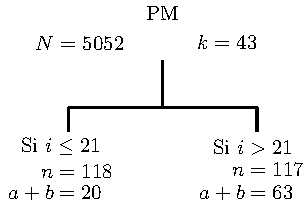
\includegraphics[width=4cm]{Graficos/e-figura1}
		
		%%
		%
		%	CAMBIAAAAAAAR
		%
		\caption{}
		\label{fig:e-figura1}
	\end{figure}
\end{observ}

\begin{observ}
	En el ejemplo \eqref{ejem-6.2}, el tamaño de la muestra obtenida con muestreo aleatorio simple es igual a \(115\), que por los ajustes necesarios en el muestreo sistemático aplicado, el tamaño de la muestra es igual a \(117\) o \(118\), dependiendo del elemento de inicio \(i\).
	
	Aparentemente, la diferencia en el tamaño de la muestra no es significativa; pero, en ciertos procesos es indispensable realizar esos ajustes para evitar que al final se pierda información de elementos que podrían representar cambios en la calidad de la producción. Por ejemplo, en la fabricación de piezas con maquinaria posible de recalentamiento o el tipo de materia prima utilizada.
\end{observ}

\begin{observ}
	Es conveniente presentar en la figura resumen, como la figura \eqref{fig:e-figura1}, el resultado de \(a+b\) dependiendo del valor de inicio \(i\) podría ser significativo para los interesados, tomar un elemento aleatorio adicional al principio o al final por cuestiones de calidad o un mejor conocimiento del comportamiento de los elementos de la población.
	
	
	En el ejemplo \eqref{ejem-6.2}.
	
	Si aleatoriamente se inicia en el elemento \(18\), \(a=17\) y \(b=3\). Podría ser de interés tomar aleatoriamente un elemento adicional entre los primeros 17 para analizar cómo comienza el proceso de producción o servicio.
	
	Si aleatoriamente se inicia en el elemento 25. \(a=24\) y \(b=39\). Podría ser de interés tomar aleatoriamente un elemento adicional entre los 39 últimos para analizar cómo culmina el proceso de producción o servicio.
	
	Eso se debe analizar considerando los costos o tiempo que representa incrementar adicionalmente
	un elemento en el proceso de muestreo sistemático.
\end{observ}


\begin{ejem}
	En un proceso de producción de 2236 unidades se conoce que la desviación estándar del proceso es igual a 6.4 libras. Obtenga el plan de muestreo sistemático si el límite para el error de estimación para la media del proceso es igual a 1.33 libras.
\end{ejem}
\begin{proof}[Solución]
		\(N=2236\); \(\sigma=6.4\); \(B=1.33\). No hay fija el nivel de confianza, se supone \(\gamma=0.95\),
		
		\(B=z_{\nicefrac{\alpha}{2}}\sqrt{\hat{\Var}[\bar{X}]}=\dfrac{\sigma^2}{n}\left(\dfrac{N-n}{N-1}\right)\); \(B=z_{\nicefrac{\alpha}{2}}\sqrt{\dfrac{\sigma^2(N-n)}{n(N-1)}}\); 
		
		\(P(Z<z_{\nicefrac{\alpha}{2}})=0.975\); \(z_{\nicefrac{\alpha}{2}}=1.96\);
		
		\(n=\dfrac{z_{\nicefrac{\alpha}{2}}\sigma^2N}{B^2(N-1)+z_{\nicefrac{\alpha}{2}}^2\sigma^2}=\dfrac{1.96^2 \times 6.4^2 \times 2236}{1.33^2 \times 2235+1.96^2 \times 6.4^2}=85.588\); \(n=86\)
		
		\(\dfrac{N}{n}=\dfrac{2236}{26}=26\); \(k=26\); \(e=0\); \(r=0\)
		
		No es posible incrementar una unidad en la muestra.
		
		Para comprobar lo obtenido: \(i=6\); \(a=5\); \(l=6+85 \times 26=2216\); \(b=2236-2216=20\); \(a+b=25\). No es posible incrementar una unidad en la muestra.
		
		PM: \(N=2236\); \(n=86\); \(k=26\)
\end{proof}

\begin{ejem}
	En la segunda parte del problema del ejemplo \eqref{ejem-5.7} se ha resuelto tomar la muestra sistemáticamente. Obtenga el plan de muestreo sistemático que garantice la participación de la mayor cantidad posible de elementos de la población.
\end{ejem}
\begin{proof}[Solución]\qquad
	
		\(N=365\); \(n=43\)
		
		\(\dfrac{N}{n}=\dfrac{365}{43}=8.488\); \(k=8\); \(e=0.488\); \(r=42 \times e=20.5116\)
		
		\(\left[\dfrac{r}{k}\right]=\left[\dfrac{20.5116}{8}\right]=[2.5639]=2\). De aproximadamente \(20\) elementos de la población se pueden tomar \(2\) de cada \(8\); por lo tanto \(n=45\).
		
		\(\dfrac{N}{n}=\dfrac{365}{45}=8.1111\); \(k=8\); \(e=0.1111\); \(r=44 \times e=4.888\)
		
		Como \(r=4.888<k=8\), se incrementa un elemento en la muestra hasta cierto \(i\).
		
		Tomando un elemento \(i\leq k\); por el ejemplo \(i=3\), \(a=2\);
		\(l=i+(n-1) \times k=3+44 \times 8=355\); \(b=N-l=365-355=10\); \(a+b=2+10=12\); se ratifica que se incrementa un elemento en la muestra hasta cierto \(i\).
		
		¿Hasta qué \(i\) se incrementa la muestra en una unidad?
		Hasta \(i=a+b-k+1=12-8+1=5\), o, \(i=N-nk=365-45 \times 8=5\)	\qedhere
		\begin{figure}[H]
			\centering
			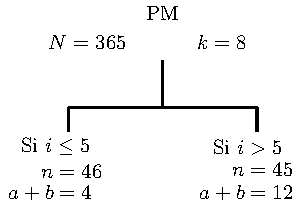
\includegraphics[width=4.5cm]{Graficos/e-figura2}
%			\caption{}
%			\label{fig:e-figura2}
		\end{figure}
		
\end{proof}


\begin{ejem}
	Por muestreo piloto anterior se conoce que el \(63\%\) de las \(4556\) personas están de acuerdo con la atención que reciben en el centro comercial donde realizan sus compras.
	
	Para realizar el estudio definitivo se ha fijado que el límite para el error de estimación para la proporción de personas que están de acuerdo con la atención que reciben sea igual al \(4.73\%\) y que el nivel de confianza sea igual al \(90\%\). Obtenga el plan de muestreo sistemático que garantice la participación de la mayor cantidad posible de elementos de la población.
\end{ejem}
\begin{proof}[Solución]
		\(N=4556\); \(\hat{p}=0.63\); \(B=0.473\); \(\gamma=0.90\); \(P(Z>z_{\nicefrac{\alpha}{2}})=0.95\); \(z_{\nicefrac{\alpha}{2}}=1.645\)
		
		\(B=z_{\nicefrac{\alpha}{2}}\sqrt{\hat{\Var}[\hat{P}]}\); \(\hat{\Var}[\hat{P}]=\dfrac{\hat{p}\hat{q}}{n-1}\left(\dfrac{N-n}{N}\right)\); \(B=z_{\nicefrac{\alpha}{2}}\sqrt{\dfrac{\hat{p}\hat{q}(N-n)}{(n-1)N}}\); \(n=\dfrac{z_{\nicefrac{\alpha}{2}}^2\hat{p}\hat{q} N+B^2N}{B^2N+z_{\nicefrac{\alpha}{2}}^2\hat{p}\hat{q}}\)
		
		\(n=\dfrac{1.645^2 \times 0.63 \times 0.37 \times 4556+0.0473^2 \times 4556}{0.0473^2 \times 4556+1.645^2 \times 0.63 \times 0.37}=266.448\); \(n=267\)
		
		\(\dfrac{N}{n}=\dfrac{4556}{267}=17.0636\); \(k=17\); \(e=0.0636\); \(r=266 \times e=16.936\)
		
		Como \(r=16.936<k=17\), se incrementa un elemento en la muestra hasta cierto \(i\).
		
		Tomando \(i=8\), \(a=7\); \(l=i+(n-1) \times k=8+266 \times 17=4530\); \(b=N-l=4556-4530=26\); \(a+b=7+26=33\); se ratifica que se incrementa un elemento en la muestra hasta cierto  \(i\).
		
		¿Hasta qué \(i\) se incrementa la muestra en una unidad?
		
		Hasta \(i=a+b-k+1=33-17+1=17\), o, \(i=N-nk=4556-267 \times 17=17\).
		
		Por lo tanto PM: \(N=4556\); \(n=268\); \(k=17\).
\end{proof}


\nocite{E-1, E-2, E-3, E-4, E-5}
}

\newpage




\begin{table}[H]
\fontsize{6.5}{7.5}\selectfont
\captionsetup{justification=centering, labelfont=footnotesize, font=footnotesize}
  \centering
  \vspace{-2.5em}
  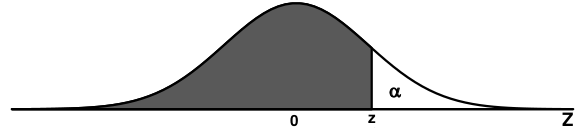
\includegraphics[width=0.55\linewidth]{Graficos/e-d-n}
%
	\[F(z)=P(Z\leq z)=\int_{-\infty}^{z}\dfrac{1}{\sqrt{2\pi}}e^{\nicefrac{t^2}{2}}=1-\alpha\]
    \begin{tabular}{c | cccccccccccc} \thickline
	$z$ & 0.00&0.01&0.02&0.03&0.04&0.05&0.06&0.07&0.08&0.09
    \\ \hline
	0.0&0.5000&0.5040&0.5080&0.5120&0.5160&0.5199&0.5239&0.5279&0.5319&0.5359    \\
	0.1&0.5398&0.5438&0.5478&0.5517&0.5557&0.5596&0.5636&0.5675&0.5714&0.5753	\\
	0.2&0.5793&0.5832&0.5871&0.5910&0.5948&0.5987&0.6026&0.6064&0.6103&0.6141	\\
	0.3&0.6179&0.6217&0.6255&0.6293&0.6331&0.6368&0.6406&0.6443&0.6480&0.6517	\\
	0.4&0.6554&0.6591&0.6628&0.6664&0.6700&0.6736&0.6772&0.6808&0.6844&0.6879	\\
	0.5&0.6915&0.6950&0.6985&0.7019&0.7054&0.7088&0.7123&0.7157&0.7190&0.7224	\\
	0.6&0.7257&0.7291&0.7324&0.7357&0.7389&0.7422&0.7454&0.7486&0.7517&0.7549	\\
	0.7&0.7580&0.7611&0.7642&0.7673&0.7703&0.7734&0.7764&0.7794&0.7823&0.7852	\\
	0.8&0.7881&0.7910&0.7939&0.7967&0.7995&0.8023&0.8051&0.8078&0.8106&0.8133	\\
	0.9&0.8159&0.8186&0.8212&0.8238&0.8264&0.8289&0.8315&0.8340&0.8365&0.8389	\\
	1.0&0.8413&0.8438&0.8461&0.8485&0.8508&0.8531&0.8554&0.8577&0.8599&0.8621	\\
	1.1&0.8643&0.8665&0.8686&0.8708&0.8729&0.8749&0.8770&0.8790&0.8810&0.8830	\\
	1.2&0.8849&0.8869&0.8888&0.8907&0.8925&0.8944&0.8962&0.8980&0.8997&0.9015	\\
	1.3&0.9032&0.9049&0.9066&0.9082&0.9099&0.9115&0.9131&0.9147&0.9162&0.9177	\\
	1.4&0.9192&0.9207&0.9222&0.9236&0.9251&0.9265&0.9279&0.9292&0.9306&0.9319	\\
	1.5&0.9332&0.9345&0.9357&0.9370&0.9382&0.9394&0.9406&0.9418&0.9429&0.9441	\\
	1.6&0.9452&0.9463&0.9474&0.9484&0.9495&0.9505&0.9515&0.9525&0.9535&0.9545	\\
	1.7&0.9554&0.9564&0.9573&0.9582&0.9591&0.9599&0.9608&0.9616&0.9625&0.9633	\\
	1.8&0.9641&0.9649&0.9656&0.9664&0.9671&0.9678&0.9686&0.9693&0.9699&0.9706	\\
	1.9&0.9713&0.9719&0.9726&0.9732&0.9738&0.9744&0.9750&0.9756&0.9761&0.9767	\\
	2.0&0.9772&0.9778&0.9783&0.9788&0.9793&0.9798&0.9803&0.9808&0.9812&0.9817	\\
	2.1&0.9821&0.9826&0.9830&0.9834&0.9838&0.9842&0.9846&0.9850&0.9854&0.9857	\\
	2.2&0.9861&0.9864&0.9868&0.9871&0.9875&0.9878&0.9881&0.9884&0.9887&0.9890	\\
	2.3&0.9893&0.9896&0.9898&0.9901&0.9904&0.9906&0.9909&0.9911&0.9913&0.9916	\\
	2.4&0.9918&0.9920&0.9922&0.9925&0.9927&0.9929&0.9931&0.9932&0.9934&0.9936	\\
	2.5&0.9938&0.9940&0.9941&0.9943&0.9945&0.9946&0.9948&0.9949&0.9951&0.9952	\\
	2.6&0.9953&0.9955&0.9956&0.9957&0.9959&0.9960&0.9961&0.9962&0.9963&0.9964	\\
	2.7&0.9965&0.9966&0.9967&0.9968&0.9969&0.9970&0.9971&0.9972&0.9973&0.9974	\\
	2.8&0.9974&0.9975&0.9976&0.9977&0.9977&0.9978&0.9979&0.9979&0.9980&0.9981	\\
	2.9&0.9981&0.9982&0.9982&0.9983&0.9984&0.9984&0.9985&0.9985&0.9986&0.9986	\\
	3.0&0.9987&0.9987&0.9987&0.9988&0.9988&0.9989&0.9989&0.9989&0.9990&0.9990	\\
	3.1&0.9990&0.9991&0.9991&0.9991&0.9992&0.9992&0.9992&0.9992&0.9993&0.9993	\\
	3.2&0.9993&0.9993&0.9994&0.9994&0.9994&0.9994&0.9994&0.9995&0.9995&0.9995	\\
	3.3&0.9995&0.9995&0.9995&0.9996&0.9996&0.9996&0.9996&0.9996&0.9996&0.9997	\\
	3.4&0.9997&0.9997&0.9997&0.9997&0.9997&0.9997&0.9997&0.9997&0.9997&0.9998	\\
	3.5&0.9998&0.9998&0.9998&0.9998&0.9998&0.9998&0.9998&0.9998&0.9998&0.9998	\\
	3.6&0.9998&0.9998&0.9999&0.9999&0.9999&0.9999&0.9999&0.9999&0.9999&0.9999	\\
	3.7&0.9999&0.9999&0.9999&0.9999&0.9999&0.9999&0.9999&0.9999&0.9999&0.9999	\\
	3.8&0.9999&0.9999&0.9999&0.9999&0.9999&0.9999&0.9999&0.9999&0.9999&0.9999	\\
	3.9&1.0000&1.0000&1.0000&1.0000&1.0000&1.0000&1.0000&1.0000&1.0000&1.0000\\	
    \thickline
    \end{tabular}
    \caption{Distribución Normal}
\end{table}

\newpage
\newgeometry{top=2cm, bottom=2cm, left=1cm, right=1cm, headheight=1.8cm,headsep=.5cm,footskip=1.3cm}
	

\begin{table}[H]
\setlength{\tabcolsep}{1.5pt}
%\renewcommand{\arraystretch}{1}

\fontsize{6}{7}\selectfont
\captionsetup{justification=centering, labelfont=footnotesize, font=footnotesize}
  \centering
  \vspace{-2.5em}
  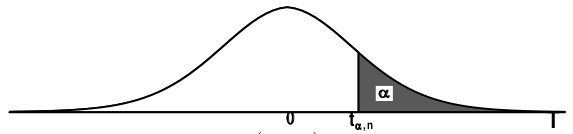
\includegraphics[width=0.55\linewidth]{Graficos/e-d-t}
%
	\[F(z)=P(T\geq t_{\alpha,n})=\alpha\]
    \begin{tabular}{c | ccccccccccccccccc} 
    \thickline
	\multirow{2}{*}{$\nu$} & \multicolumn{17}{c}{\(\alpha\)}
	\\
&0.200&0.150&0.100&0.090&0.080&0.070&0.060&0.050&0.045&0.040&0.035&0.030&0.025&0.020&0.015&0.010&0.005
    \\ \hline
	%
1&1.3764&1.9626&3.0777&3.4420&3.8947&4.4737&5.2422&6.3138&7.0264&7.9158&9.0579&10.579&12.706&15.895&21.205&31.821&63.657
\\
2&1.0607&1.3862&1.8856&2.0261&2.1894&2.3834&2.6202&2.9200&3.1040&3.3198&3.5782&3.8964&4.3027&4.8487&5.6428&6.9646&9.9248
\\
3&0.9785&1.2498&1.6377&1.7413&1.8589&1.9950&2.1562&2.3534&2.4708&2.6054&2.7626&2.9505&3.1824&3.4819&3.8960&4.5407&5.8409
\\
4&0.9410&1.1896&1.5332&1.6226&1.7229&1.8375&1.9712&2.1318&2.2261&2.3329&2.4559&2.6008&2.7764&2.9985&3.2976&3.7469&4.6041\\
5&0.9195&1.1558&1.4759&1.5579&1.6493&1.7529&1.8727&2.0150&2.0978&2.1910&2.2974&2.4216&2.5706&2.7565&3.0029&3.3649&4.0321\\
6&0.9057&1.1342&1.4398&1.5172&1.6033&1.7002&1.8117&1.9432&2.0192&2.1043&2.2011&2.3133&2.4469&2.6122&2.8289&3.1427&3.7074\\
7&0.8960&1.1192&1.4149&1.4894&1.5718&1.6643&1.7702&1.8946&1.9662&2.0460&2.1365&2.2409&2.3646&2.5168&2.7146&2.9980&3.4995\\
8&0.8889&1.1081&1.3968&1.4691&1.5489&1.6383&1.7402&1.8595&1.9280&2.0042&2.0902&2.1892&2.3060&2.4490&2.6338&2.8965&3.3554\\
9&0.8834&1.0997&1.3830&1.4537&1.5315&1.6185&1.7176&1.8331&1.8992&1.9727&2.0554&2.1504&2.2622&2.3984&2.5738&2.8214&3.2498\\
10&0.8791&1.0931&1.3722&1.4416&1.5179&1.6031&1.6998&1.8125&1.8768&1.9481&2.0283&2.1202&2.2281&2.3593&2.5275&2.7638&3.1693\\
11&0.8755&1.0877&1.3634&1.4318&1.5069&1.5906&1.6856&1.7959&1.8588&1.9284&2.0067&2.0961&2.2010&2.3281&2.4907&2.7181&3.1058\\
12&0.8726&1.0832&1.3562&1.4237&1.4979&1.5804&1.6739&1.7823&1.8440&1.9123&1.9889&2.0764&2.1788&2.3027&2.4607&2.6810&3.0545\\
13&0.8702&1.0795&1.3502&1.4170&1.4903&1.5718&1.6641&1.7709&1.8317&1.8989&1.9742&2.0600&2.1604&2.2816&2.4358&2.6503&3.0123\\
14&
0.8681&
1.0763&
1.3450&
1.4113&
1.4839&
1.5646&
1.6558&
1.7613&
1.8213&
1.8875&
1.9617&
2.0462&
2.1448&
2.2638&
2.4149&
2.6245&
2.9768\\
15&
0.8662&
1.0735&
1.3406&
1.4063&
1.4784&
1.5583&
1.6487&
1.7531&
1.8123&
1.8777&
1.9509&
2.0343&
2.1314&
2.2485&
2.3970&
2.6025&
2.9467\\
16&
0.8647&
1.0711&
1.3368&
1.4021&
1.4736&
1.5529&
1.6425&
1.7459&
1.8046&
1.8693&
1.9417&
2.0240&
2.1199&
2.2354&
2.3815&
2.5835&
2.9208\\
17&
0.8633&
1.0690&
1.3334&
1.3983&
1.4694&
1.5482&
1.6370&
1.7396&
1.7978&
1.8619&
1.9335&
2.0150&
2.1098&
2.2238&
2.3681&
2.5669&
2.8982\\
18&
0.8620&
1.0672&
1.3304&
1.3950&
1.4656&
1.5439&
1.6322&
1.7341&
1.7918&
1.8553&
1.9264&
2.0071&
2.1009&
2.2137&
2.3562&
2.5524&
2.8784\\
19&
0.8610&
1.0655&
1.3277&
1.3920&
1.4623&
1.5402&
1.6280&
1.7291&
1.7864&
1.8495&
1.9200&
2.0000&
2.0930&
2.2047&
2.3456&
2.5395&
2.8609\\
20&
0.8600&
1.0640&
1.3253&
1.3894&
1.4593&
1.5369&
1.6242&
1.7247&
1.7816&
1.8443&
1.9143&
1.9937&
2.0860&
2.1967&
2.3362&
2.5280&
2.8453\\
21&
0.8591&
1.0627&
1.3232&
1.3870&
1.4567&
1.5338&
1.6207&
1.7207&
1.7773&
1.8397&
1.9092&
1.9880&
2.0796&
2.1894&
2.3278&
2.5176&
2.8314\\
22&
0.8583&
1.0614&
1.3212&
1.3848&
1.4542&
1.5311&
1.6176&
1.7171&
1.7734&
1.8354&
1.9045&
1.9829&
2.0739&
2.1829&
2.3202&
2.5083&
2.8188\\
23&
0.8575&
1.0603&
1.3195&
1.3828&
1.4520&
1.5286&
1.6148&
1.7139&
1.7699&
1.8316&
1.9003&
1.9782&
2.0687&
2.1770&
2.3132&
2.4999&
2.8073\\
24&
0.8569&
1.0593&
1.3178&
1.3810&
1.4500&
1.5263&
1.6122&
1.7109&
1.7667&
1.8281&
1.8965&
1.9740&
2.0639&
2.1715&
2.3069&
2.4922&
2.7969\\
25&
0.8562&
1.0584&
1.3163&
1.3794&
1.4482&
1.5242&
1.6098&
1.7081&
1.7637&
1.8248&
1.8929&
1.9701&
2.0595&
2.1666&
2.3011&
2.4851&
2.7874\\
26&
0.8557&
1.0575&
1.3150&
1.3778&
1.4464&
1.5223&
1.6076&
1.7056&
1.7610&
1.8219&
1.8897&
1.9665&
2.0555&
2.1620&
2.2958&
2.4786&
2.7787\\
27&
0.8551&
1.0567&
1.3137&
1.3764&
1.4449&
1.5205&
1.6056&
1.7033&
1.7585&
1.8191&
1.8867&
1.9632&
2.0518&
2.1578&
2.2909&
2.4727&
2.7707\\
28&
0.8546&
1.0560&
1.3125&
1.3751&
1.4434&
1.5189&
1.6037&
1.7011&
1.7561&
1.8166&
1.8839&
1.9601&
2.0484&
2.1539&
2.2864&
2.4671&
2.7633\\
29&
0.8542&
1.0553&
1.3114&
1.3739&
1.4421&
1.5174&
1.6020&
1.6991&
1.7540&
1.8142&
1.8813&
1.9573&
2.0452&
2.1503&
2.2822&
2.4620&
2.7564\\
30&
0.8538&
1.0547&
1.3104&
1.3728&
1.4408&
1.5159&
1.6004&
1.6973&
1.7520&
1.8120&
1.8789&
1.9546&
2.0423&
2.1470&
2.2783&
2.4573&
2.7500\\
35&
0.8520&
1.0520&
1.3062&
1.3681&
1.4356&
1.5101&
1.5937&
1.6896&
1.7436&
1.8030&
1.8691&
1.9438&
2.0301&
2.1332&
2.2622&
2.4377&
2.7238\\
40&
0.8507&
1.0500&
1.3031&
1.3646&
1.4317&
1.5057&
1.5887&
1.6839&
1.7375&
1.7963&
1.8617&
1.9357&
2.0211&
2.1229&
2.2503&
2.4233&
2.7045\\
45&
0.8497&
1.0485&
1.3006&
1.3619&
1.4287&
1.5023&
1.5849&
1.6794&
1.7327&
1.7911&
1.8561&
1.9294&
2.0141&
2.1150&
2.2411&
2.4121&
2.6896\\
50&
0.8489&
1.0473&
1.2987&
1.3598&
1.4263&
1.4996&
1.5818&
1.6759&
1.7289&
1.7870&
1.8516&
1.9244&
2.0086&
2.1087&
2.2338&
2.4033&
2.6778\\
55&
0.8482&
1.0463&
1.2971&
1.3580&
1.4243&
1.4974&
1.5793&
1.6730&
1.7258&
1.7836&
1.8479&
1.9204&
2.0040&
2.1036&
2.2278&
2.3961&
2.6682\\
60&
0.8477&
1.0455&
1.2958&
1.3566&
1.4227&
1.4956&
1.5772&
1.6706&
1.7232&
1.7808&
1.8448&
1.9170&
2.0003&
2.0994&
2.2229&
2.3901&
2.6603\\
65&
0.8472&
1.0448&
1.2947&
1.3553&
1.4213&
1.4941&
1.5755&
1.6686&
1.7210&
1.7785&
1.8423&
1.9142&
1.9971&
2.0958&
2.2188&
2.3851&
2.6536\\
70&
0.8468&
1.0442&
1.2938&
1.3543&
1.4202&
1.4927&
1.5740&
1.6669&
1.7192&
1.7765&
1.8401&
1.9118&
1.9944&
2.0927&
2.2152&
2.3808&
2.6479\\
75&
0.8464&
1.0436&
1.2929&
1.3534&
1.4191&
1.4916&
1.5727&
1.6654&
1.7176&
1.7747&
1.8381&
1.9097&
1.9921&
2.0901&
2.2122&
2.3771&
2.6430\\
80&
0.8461&
1.0432&
1.2922&
1.3526&
1.4183&
1.4906&
1.5716&
1.6641&
1.7162&
1.7732&
1.8365&
1.9078&
1.9901&
2.0878&
2.2095&
2.3739&
2.6387
\\
    \thickline
    \end{tabular}
    \caption{Distribución \(t\) de Student -- (a)}
\end{table}	
	
\begin{table}[H]
\setlength{\tabcolsep}{1.5pt}
%\renewcommand{\arraystretch}{1}

\fontsize{6}{7}\selectfont
\captionsetup{justification=centering, labelfont=footnotesize, font=footnotesize}
  \centering
  \vspace{-2.5em}
  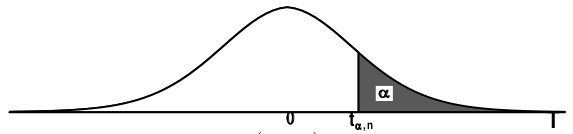
\includegraphics[width=0.55\linewidth]{Graficos/e-d-t}
%
	\[F(z)=P(T\geq t_{\alpha,n})=\alpha\]
    \begin{tabular}{c | ccccccccccccccccc} 
    \thickline
	\multirow{2}{*}{$\nu$} & \multicolumn{17}{c}{\(\alpha\)}
	\\
&0.200&0.150&0.100&0.090&0.080&0.070&0.060&0.050&0.045&0.040&0.035&0.030&0.025&0.020&0.015&0.010&0.005
    \\ \hline
	%
85&
0.8459&
1.0428&
1.2916&
1.3519&
1.4175&
1.4897&
1.5706&
1.6630&
1.7149&
1.7719&
1.8350&
1.9062&
1.9883&
2.0857&
2.2071&
2.3710&
2.6349\\
90&
0.8456&
1.0424&
1.2910&
1.3513&
1.4168&
1.4889&
1.5697&
1.6620&
1.7138&
1.7707&
1.8337&
1.9048&
1.9867&
2.0839&
2.2050&
2.3685&
2.6316\\
95&
0.8454&
1.0421&
1.2905&
1.3507&
1.4162&
1.4882&
1.5689&
1.6611&
1.7129&
1.7696&
1.8326&
1.9035&
1.9853&
2.0823&
2.2032&
2.3662&
2.6286\\
100&
0.8452&
1.0418&
1.2901&
1.3502&
1.4156&
1.4876&
1.5682&
1.6602&
1.7120&
1.7687&
1.8315&
1.9024&
1.9840&
2.0809&
2.2015&
2.3642&
2.6259\\
105&
0.8451&
1.0416&
1.2897&
1.3497&
1.4151&
1.4870&
1.5675&
1.6595&
1.7112&
1.7678&
1.8306&
1.9013&
1.9828&
2.0796&
2.2000&
2.3624&
2.6235\\
110&
0.8449&
1.0413&
1.2893&
1.3493&
1.4146&
1.4865&
1.5669&
1.6588&
1.7105&
1.7670&
1.8297&
1.9004&
1.9818&
2.0784&
2.1986&
2.3607&
2.6213\\
115&
0.8448&
1.0411&
1.2890&
1.3490&
1.4142&
1.4861&
1.5664&
1.6582&
1.7098&
1.7663&
1.8289&
1.8995&
1.9808&
2.0773&
2.1974&
2.3592&
2.6193\\
120&
0.8446&
1.0409&
1.2886&
1.3486&
1.4138&
1.4856&
1.5659&
1.6577&
1.7092&
1.7656&
1.8282&
1.8987&
1.9799&
2.0763&
2.1962&
2.3578&
2.6174\\
125&
0.8445&
1.0408&
1.2884&
1.3483&
1.4135&
1.4852&
1.5655&
1.6571&
1.7086&
1.7650&
1.8276&
1.8980&
1.9791&
2.0754&
2.1951&
2.3565&
2.6157\\
130&
0.8444&
1.0406&
1.2881&
1.3480&
1.4132&
1.4849&
1.5651&
1.6567&
1.7081&
1.7645&
1.8270&
1.8973&
1.9784&
2.0746&
2.1942&
2.3554&
2.6142\\
135&
0.8443&
1.0404&
1.2879&
1.3477&
1.4129&
1.4845&
1.5647&
1.6562&
1.7076&
1.7640&
1.8264&
1.8967&
1.9777&
2.0738&
2.1933&
2.3543&
2.6127\\
140&
0.8442&
1.0403&
1.2876&
1.3475&
1.4126&
1.4842&
1.5643&
1.6558&
1.7072&
1.7635&
1.8259&
1.8962&
1.9771&
2.0731&
2.1924&
2.3533&
2.6114\\
145&
0.8441&
1.0402&
1.2874&
1.3473&
1.4123&
1.4839&
1.5640&
1.6554&
1.7068&
1.7630&
1.8254&
1.8956&
1.9765&
2.0724&
2.1917&
2.3523&
2.6102\\
150&
0.8440&
1.0400&
1.2872&
1.3470&
1.4121&
1.4836&
1.5637&
1.6551&
1.7064&
1.7626&
1.8249&
1.8951&
1.9759&
2.0718&
2.1909&
2.3515&
2.6090\\
169&
0.8438&
1.0396&
1.2866&
1.3463&
1.4113&
1.4828&
1.5627&
1.6539&
1.7052&
1.7613&
1.8235&
1.8935&
1.9741&
2.0697&
2.1886&
2.3486&
2.6052\\
188&
0.8435&
1.0393&
1.2861&
1.3458&
1.4107&
1.4821&
1.5619&
1.6530&
1.7042&
1.7602&
1.8223&
1.8922&
1.9727&
2.0681&
2.1867&
2.3463&
2.6022\\
207&
0.8434&
1.0390&
1.2857&
1.3453&
1.4101&
1.4815&
1.5612&
1.6522&
1.7034&
1.7593&
1.8213&
1.8912&
1.9715&
2.0668&
2.1852&
2.3445&
2.5998\\
226&
0.8432&
1.0388&
1.2853&
1.3449&
1.4097&
1.4810&
1.5607&
1.6516&
1.7027&
1.7586&
1.8205&
1.8903&
1.9705&
2.0657&
2.1839&
2.3430&
2.5978\\
245&
0.8431&
1.0386&
1.2850&
1.3446&
1.4093&
1.4806&
1.5602&
1.6511&
1.7021&
1.7580&
1.8199&
1.8895&
1.9697&
2.0647&
2.1828&
2.3417&
2.5960\\
264&
0.8430&
1.0385&
1.2848&
1.3443&
1.4090&
1.4802&
1.5598&
1.6506&
1.7016&
1.7575&
1.8193&
1.8889&
1.9690&
2.0639&
2.1819&
2.3406&
2.5946\\
283&
0.8429&
1.0383&
1.2846&
1.3441&
1.4088&
1.4799&
1.5595&
1.6503&
1.7012&
1.7570&
1.8188&
1.8884&
1.9684&
2.0633&
2.1811&
2.3396&
2.5933\\
302&
0.8428&
1.0382&
1.2844&
1.3439&
1.4085&
1.4797&
1.5592&
1.6499&
1.7009&
1.7566&
1.8184&
1.8879&
1.9679&
2.0627&
2.1804&
2.3388&
2.5922\\
401&
0.8425&
1.0378&
1.2837&
1.3431&
1.4077&
1.4787&
1.5581&
1.6487&
1.6995&
1.7551&
1.8168&
1.8861&
1.9659&
2.0605&
2.1778&
2.3357&
2.5881\\
500&
0.8423&
1.0375&
1.2832&
1.3426&
1.4072&
1.4781&
1.5574&
1.6479&
1.6987&
1.7543&
1.8158&
1.8851&
1.9647&
2.0591&
2.1763&
2.3338&
2.5857\\
599&
0.8422&
1.0373&
1.2830&
1.3423&
1.4068&
1.4778&
1.5570&
1.6474&
1.6981&
1.7537&
1.8152&
1.8844&
1.9639&
2.0582&
2.1753&
2.3326&
2.5841\\
\(\infty\)&
0.8416&
1.0364&
1.2816&
1.3408&
1.4051&
1.4758&
1.5548&
1.6449&
1.6954&
1.7507&
1.8119&
1.8808&
1.9600&
2.0538&
2.1701&
2.3264&
2.5758
\\
    \thickline
    \end{tabular}
    \caption{Distribución \(t\) de Student -- (b)}
\end{table}		
	
	
	

%
%
%
%
%
%
%
%
%
%
%
%
%
%
%
%
%
%
%
%
%
%
%
%
%
%
%
%
%
%
%
%
%
%

\vfill
\newpage
\newgeometry{top=2cm, bottom=2cm, left=2cm, right=2cm, headheight=1.8cm,headsep=.5cm,footskip=1.3cm}


% ------------------ Menthor ------------------%
\Tutorial{Introducción a la teoría de estabilidad: sistemas de ecuaciones diferenciales ordinarias}{Ménthor Urvina}{\EPN, Ecuador}{menthor.urvina@epn.edu.ec}{

\vspace{1\baselineskip}\setcounter{figure}{0} \setcounter{teorema}{0} \setcounter{definicion}{0} \setcounter{proposicion}{0}
\setcounter{ejem}{0} \setcounter{observ}{0}

En el documento se presentan las principales definiciones usadas en estabilidad: sistemas autónomos, plano de fase, puntos críticos, estabilidad; así como los principales resultados para determinar la naturaleza de los puntos críticos y su estabilidad.

\subsubsection{Sistemas autónomos, el plano de fase}

A menudo sucede que muchas ecuaciones diferenciales ordinarias (o sistemas de ecuaciones diferenciales ordinarias) no pueden resolverse analíticamente en forma explícita, pero se puede analizar el comportamiento cualitativo de sus soluciones, sin el conocimiento explícito de ellas.

En lo que sigue se estudian sistemas de ecuaciones diferenciales ordinarias de la forma:
\begin{equation}\label{m-1}
	\begin{cases}
		\dfrac{dx}{dt}=F(x,y) ,\vspace{0.3em}
		\\
		\dfrac{dy}{dt}=G(x,y),
	\end{cases}
\end{equation}
donde \(F=F(x,y)\), \(G=G(x,y)\) y sus derivadas parciales son continuas en todo el plano.

EL sistema \eqref{m-1} en el que la variable  independiente \(t\) no aparece explícitamente en \(F\) y \(G\) se llama \emph{\textbf{autónomo}}.

Por el teorema de existencia y unicidad, se tiene que para cualquier \(t_0\in\R\) y \((x_0,y_0)\in\R^2\), el sistema anterior tiene una solución única: 
\begin{equation}\label{m-2}
	\begin{cases}
		x=x(t),	
		 \\
		y = y(t);
	\end{cases}
\end{equation}
que satisface la condición inicial: 
\[
	\begin{cases}
		x(t_0)=x_0,
		 \\
		y(t_0) = y_0.
	\end{cases}
\]

La solución del sistema \(\begin{cases}	x=x(t),	\\		y = y(t),	\end{cases}\) \hspace{-1em} corresponde a la representación paramétrica de una curva en el plano \(xy\), al cual se le llama plano de fase y la curva solución se denomina trayectoria del sistema, y se denota con \(\Gamma=\Gamma(x,y)=\Gamma\big(x(t),y(t)\big)\). La familia de trayectorias representadas en el plano de fase se denomina el retrato de fase.
	
\begin{observ}
	Si \eqref{m-2} es la solución de \eqref{m-1} se puede mostrar que:
	\begin{equation}\label{m-2}
	\begin{cases}
		x=x(t+c),	
		 \\
		y = y(t+c),
	\end{cases}
	\end{equation}
	también es solución del sistema, para cualquier constante \(c\), luego:
	\[
	\Gamma=\Gamma(x,y)=\Gamma\big(x(t+c),y(t+c)\big).
	\]
	Es decir cada trayectoria viene representada por muchas soluciones que difieren entre sí por una traslación del parámetro. Como el problema de valor inicial tiene solución, entonces por cada punto \((x_0,y_0)\) pasa una sola trayectoria, esto significa que las trayectorias no se intersecan.
\end{observ}

\begin{observ}\quad
	\begin{APAenumerate}
		\item La dirección \(t\) creciente a lo largo de la trayectoria dada es la misma para todas las soluciones que representa a esa trayectoria. Una trayectoria \(\Gamma=\Gamma(x,y)\)  es por tanto una curva dirigida, en los gráficos se utilizan flechas para indicar la dirección de \(t\) creciente sobre las trayectorias.
		
		\item Para los sistemas
		\[
			\begin{cases}
			x' = F(x,y),
			 \\
			y' = G(x,y),
			\end{cases}
			\yds
			\begin{cases}
			x' = -F(x,y),
			 \\
			y' = -G(x,y),
			\end{cases}
		\]
		Los diagramas de fase son los mismos, excepto que la orientación en las trayectorias se invierte.


		\item Para el punto \((x_0,y_0)\) tal que
		\(
			\begin{cases}
			x' = F(x_0,y_0)=0,
			 \\
			y' = G(x_0,y_0)=0,
			\end{cases}
		\)\hspace{-1em}
		se cumple que 
		\(
			\begin{cases}
			x(t) = x_0,
			 \\
			y(t) = y_0,
			\end{cases}
		\)\hspace{-1em}
		es también solución, pero no es una  trayectoria.
		
		
	\end{APAenumerate}
\end{observ}

De las observaciones anteriores se concluye que las trayectorias cubren todo el plano de fase y no se intersecan entre sí, la única excepción ocurre en los puntos \((x_0,y_0)\) donde \(F\) y \(G\) son cero.



\paragraph{Punto crítico}

\begin{definicion}
	Al punto \((x_0,y_0)\) que satisface \(\begin{cases}
			F(x_0,y_0)=0,
			 \\
			G(x_0,y_0)=0,
			\end{cases}
		\)\hspace{-1em}, se lo denomina \textbf{\emph{punto crítico}} del sistema.
\end{definicion}

\begin{observ}
	En los puntos críticos, la única solución del sistema es la solución constante \(x(t)=x_0\), \(y(t)=y_0\) y no define una trayectoria, así que por un punto crítico no pasa ninguna trayectoria.
	
	Se supondrá que todo punto crítico \((x_0,y_0)\) es \emph{\textbf{aislado}}, es decir, existe un círculo centrado en \((x_0,y_0)\)  que no contiene otro punto crítico.
\end{observ}

\begin{ejem}
	La ecuación del movimiento de un péndulo amortiguado es:
	\[
	\dfrac{d^2\theta}{dt^2}+\dfrac{c}{m}\dfrac{d\theta}{dt}+\dfrac{g}{a}\sen\theta=0.
	\]
	
	Tomando \(
			\begin{cases}
			x(t) = x_0,
			 \\
			y(t) = y_0,
			\end{cases}
		\)\hspace{-1em}: \(x=\theta\), \(y=\theta'\) se obtiene el sistema autónomo de ecuaciones no lineal:
	\[
		\begin{cases}
			x' = y = F(x,y),
			 \\
			y' = -\dfrac{c}{m}y-\dfrac{g}{a}\sen x=G(x,y),
			\end{cases}
	\]
	Los puntos \((n\pi,0)\) son puntos críticos aislados, ya que  \(F(n\pi,0)=G(n\pi,0)=0\). Estos puntos corresponden a un estado estacionario del cuerpo, ya que la velocidad angular \(y=\nicefrac{d\theta}{dt}\) y la aceleración angular \(\nicefrac{dy}{dt}=\nicefrac{d^2\theta}{dt^2}\)  se anulan en esos puntos, o sea la partícula está en reposo, no hay fuerza que actúe sobre ella y por consiguiente está en equilibrio. Por esta razón a los puntos críticos también se les llama puntos de equilibrio.

	Como \(x'=F(x,y)\), \(y'=G(x,y)\) son las componentes del vector tangencial a la trayectoria en el punto \(P=(x,y)\), si se considera el campo vectorial: \(V(x,y)=F(x,y)\vec{i}+G(x,y)\vec{j}\) entonces \(V\) es tangente a la trayectoria y apunta en la dirección de \(t\) creciente. Si \(t\) es el tiempo, entonces \(V\) es el vector velocidad de una partícula que se mueve sobre la trayectoria. Así, el plano de fase está lleno de partículas y cada trayectoria es la traza de una partícula precedida y seguida por otras sobre una misma trayectoria. Esto es lo que ocurre en un fluido en movimiento y como el sistema es autónomo entonces \(V(x,y)\) no cambia en el tiempo, por esta razón al movimiento del fluido se le llama \emph{\textbf{estacionario}}.

	\begin{figure}[H]
		\captionsetup{justification=centering, labelfont=footnotesize, font=footnotesize}
		\centering
		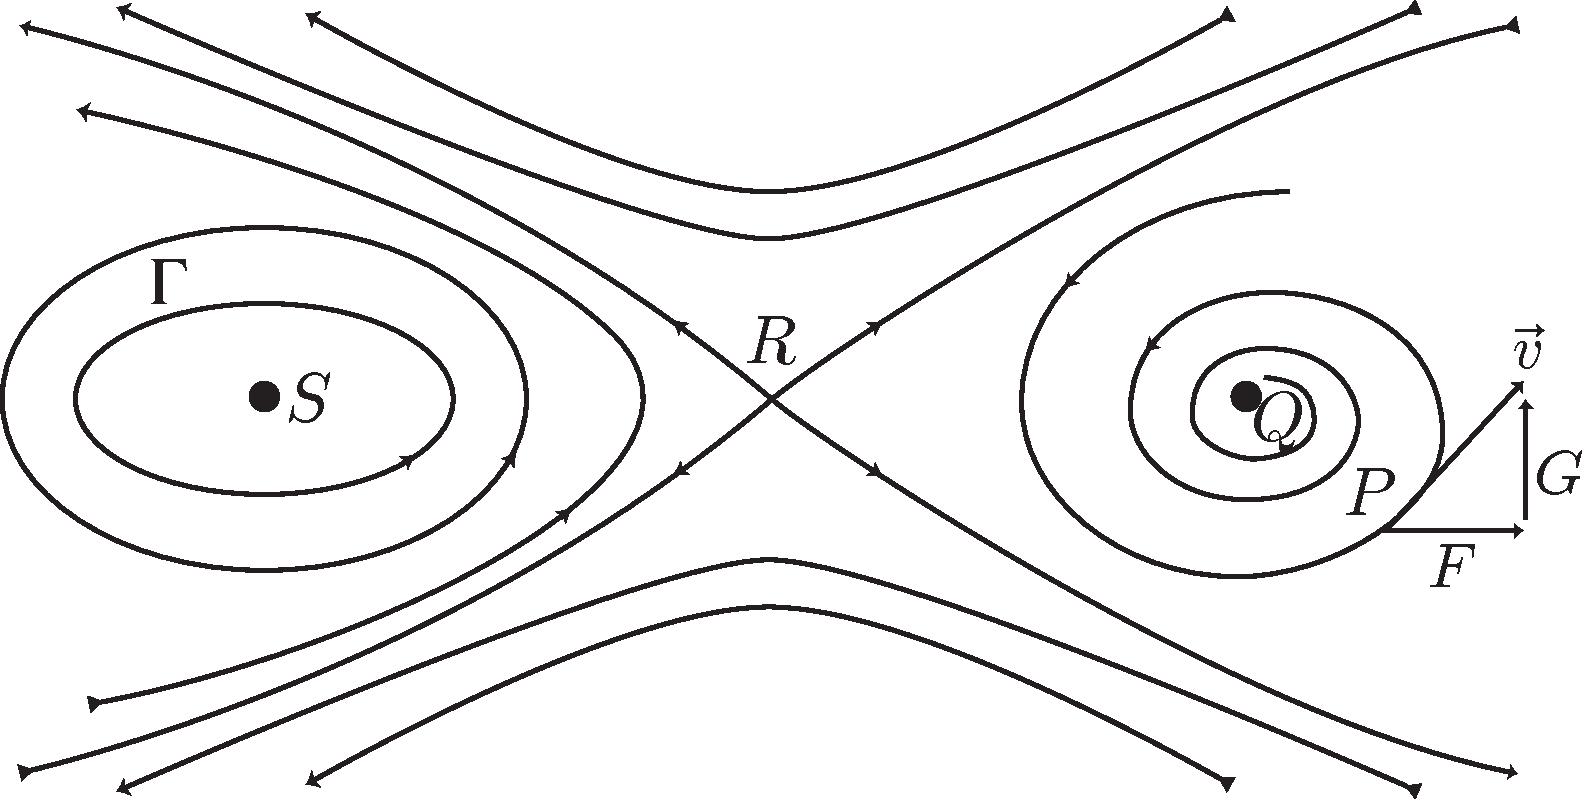
\includegraphics[width=4.5cm]{Graficos/figura1}
		\caption{ }
		\label{fig:M-1}
	\end{figure}

	
En la figura se pueden identificar lo siguiente:
	\begin{APAenumerate}
		\item Los puntos críticos,
		\item la disposición de las trayectorias cerca de los puntos críticos,
		\item la estabilidad o inestabilidad de los puntos críticos, es decir, si una partícula próxima a un punto crítico permanece cerca de él o se aleja hacia otra zona del plano,
		\item las trayectorias cerradas como la \(\Gamma\), corresponden a soluciones periódicas.
	\end{APAenumerate}

	\vspace{0.75\baselineskip}
	Como en general los sistemas no lineales no pueden resolverse explícitamente, el propósito de la teoría cualitativa siguiente es descubrir lo que sea posible acerca de los diagramas de fase a partir de las funciones \(F\) y \(G\).
\end{ejem}


%
%
%
\subsubsection{Tipos de puntos críticos y estabilidad}
%
%
%
Sea el sistema autónomo
\begin{equation}\label{m-4}
	\begin{cases}
		\dfrac{dx}{dt}=F(x,y) ,\vspace{0.3em}
		\\
		\dfrac{dy}{dt}=G(x,y),
	\end{cases}
\end{equation}
donde \(F=F(x,y)\) y \(G=G(x,y)\) son continuas, con derivadas parciales continuas en el plano de fase.

Sea \((x_0,y_0)\) un punto crítico aislado. Si \(\Gamma\big(x(t),y(t)\big)\) es una trayectoria del sistema, se dice que \(\Gamma\) tiende a \((x_0,y_0)\), cuando \(t\to\infty\) (o \(t\to-\infty\)), si:
\begin{equation}\label{m-5}
	\begin{cases}
		\lim_{t\to \infty} x(t) = x_0,
			 \\
		\lim_{t\to \infty} y(t) = y_0.
	\end{cases}
\end{equation}

\begin{observ}
	Si se cumple \eqref{m-5}, entonces \((x_0,y_0)\) es un punto crítico de \eqref{m-4}, además si \(\lim_{t\to\pm\infty}\dfrac{ y(t)-y_0}{x(t)-x_0}\), existe o es igual  a \(\pm\infty\), entonces se dice que \(\Gamma\) <<entra>> al punto crítico \((x_0,y_0)\) cuando \(t\to\infty\) o \(t\to-\infty\). Esto significa que la recta que une \((x_0,y_0)\) con \(P\) tiene una dirección determinada cuando \(t\to\infty\) o \(t\to-\infty\).
	
	Utilizando la regla de la cadena se tiene que \(\dfrac{dy}{dx}=\dfrac{G(x,y)}{F(x,y)}\) es la pendiente de la recta tangente de la trayectoria de \eqref{m-1} cuando \(F\) y \(G\) no se anulan simultáneamente; cuando se anulan simultáneamente, \((x_0,y_0)\) es un punto crítico y ninguna trayectoria pasa por él.
\end{observ}


\neodefi{Tipos de puntos críticos}


Por facilidad y sin pérdida de generalidad se supondrá que \((0,0)\) es un punto crítico.

%
\vspace{0.75\baselineskip}
	\textbf{Nodos}\newline

\vspace{-1\baselineskip}
	\begin{figure}[H]
		\captionsetup{justification=centering, labelfont=footnotesize, font=footnotesize}
		\centering
		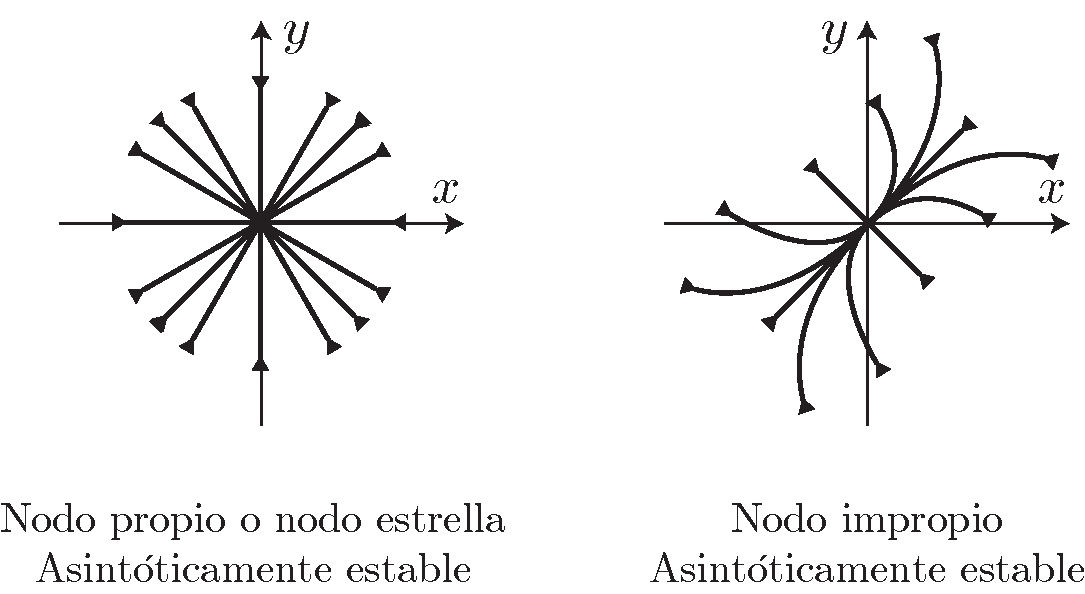
\includegraphics[scale=0.25]{Graficos/figura2}
		\caption{ }
		\label{fig:M-2}
	\end{figure}

Se distinguen dos tipos de nodos:
\begin{APAenumerate}
	\item \emph{\textbf{Nodos propios}}: en estos el retrato de fase está formado por semirectas donde todas entran (o todas salen) el punto crítico, se le llama también nodo estrella. Cuando tienden al punto cuando \(t\to\infty\), se dice que es un sumidero y cuando salen de él, o sea cuando tienden al punto cuando \(t\to-\infty\), se 	dice que es una fuente.
	
	\item \emph{\textbf{Nodo impropio}}: a un punto de este tipo tienden e incluso entran las trayectorias cuando \(t\to\infty\) (o \(t\to-\infty\)). Para este nodo existen cuatro trayectorias en forma de semirectas con extremos en el 	origen. Todas las demás trayectorias tienen el aspecto de ramas de parábola y al tender hacia el origen sus pendientes tienden a la pendiente de una de las semirectas.
\end{APAenumerate}

\vspace{-1\baselineskip}
	\begin{figure}[H]
		\captionsetup{justification=centering, labelfont=footnotesize, font=footnotesize}
		\centering
		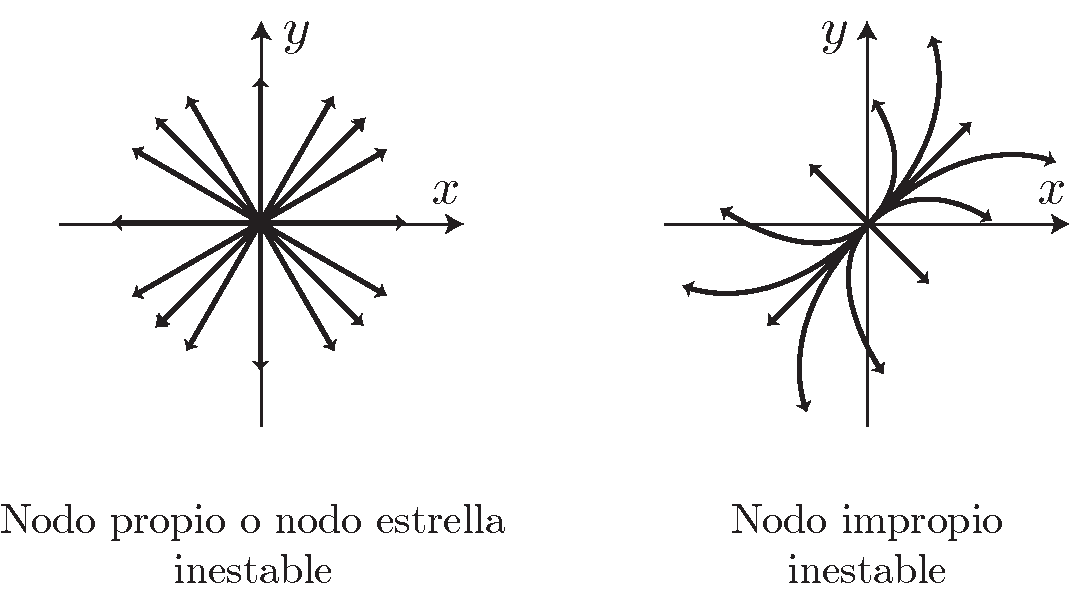
\includegraphics[scale=0.25]{Graficos/figura3}
		\caption{ }
		\label{fig:M-3}
	\end{figure}


\begin{ejem}
	Sea el sistema \(\nicefrac{dx}{dt}=x\), \(\nicefrac{dy}{dt}=-x+2y\) entonces \((0,0)\) es un punto crítico. La solución general es: 
	\[
		x(t)=c_1e^t	\yds	y(t)=c_1e^t+c_2e^{2t}.
	\]
	
	Cunado \(c_1=0 \Longrightarrow x=0\), \(y=c_2e^{2t}\) esto implica que la trayectoria es el eje \(Y\) positivo si \(c_2>0\) y el eje \(Y\) negativo si \(c_2>0\) y cada trayectoria tiende y  entra	 al origen cuando \(t\to-\infty\). Si \(c_2=0\) la trayectoria es la semirecta \(y=x\) con \(x<0\), \(c_1>0\), o también  la semirecta \(y=x\) con \(x<0\), \(c_1<0\). En estos casos ambas trayectorias tienden y entran al origen cuando \(t\to-\infty\).
	
	Si \(c_2=0\Longrightarrow x=c_1e^t\), \(y=c_1e^t\) y la trayectoria es la semirecta \(y=x\) con \(x>0\), \(c_1<0\) o también la
	semirecta \(y=x\) con \(x>0\), \(c_1>0\). En estos dos casos ambas trayectorias tienden y entran al origen cuando \(t\to-\infty\).
	
	Cuando \(c_1\neq0\), \(c_2\neq 0\), las trayectorias están sobre las parábolas \(y=x+\nicefrac{c_2}{c_1}x^2\) que entran al origen con	pendiente \(1\). Debe entenderse que estas trayectorias constan solo de una porción de la parábola, la parte con \(x>0\) si \(c_1>0\) y la parte \(x>0\) si \(c_1<0\).
	
	Nótese que \(\nicefrac{dy}{dx}=\nicefrac{(-x+2y)}{x}\): pendiente de la tangente a la trayectoria que pasa por \((x,y)\neq(0,0)\), resolviendo la EDO se encuentra \(y=x+cx^2\) que son las curvas (parábolas) sobre las que se apoyan las trayectorias, excepto las que están sobre el eje (ver figura \ref{fig:M-4}).
	
	\vspace{-1\baselineskip}
	\begin{figure}[H]
		\captionsetup{justification=centering, labelfont=footnotesize, font=footnotesize}
		\centering
		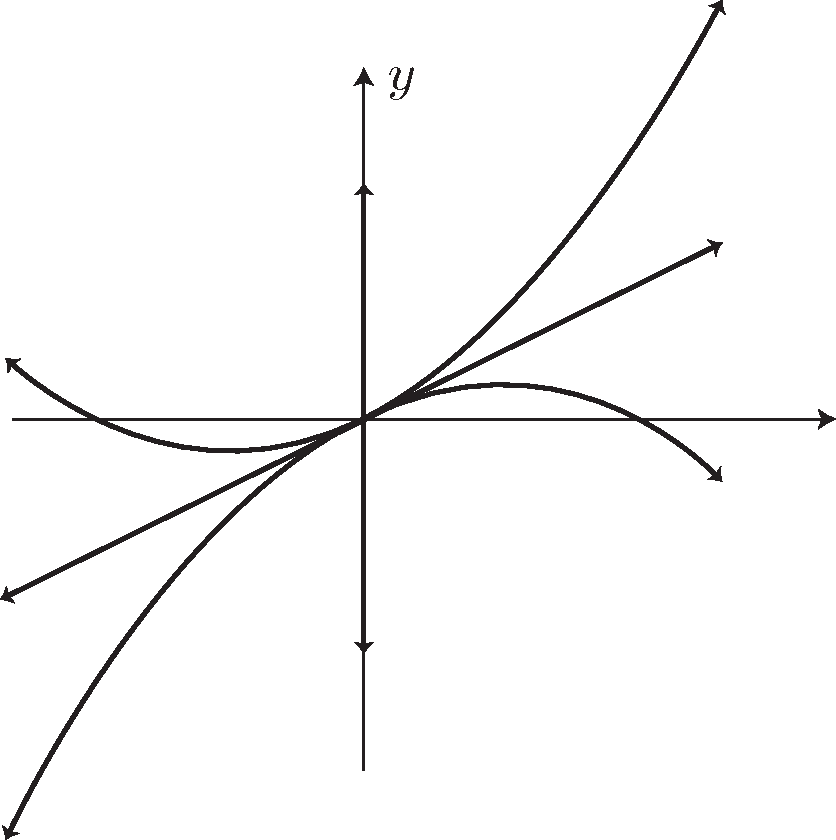
\includegraphics[width=4.5cm]{Graficos/figura4}
		\caption{Nodo impropio, inestable}
		\label{fig:M-4}
	\end{figure}
\end{ejem}



%
\vspace{0.75\baselineskip}
	\textbf{Punto de silla}\newline

\vspace{-1\baselineskip}
	\begin{figure}[H]
		\captionsetup{justification=centering, labelfont=footnotesize, font=footnotesize}
		\centering
		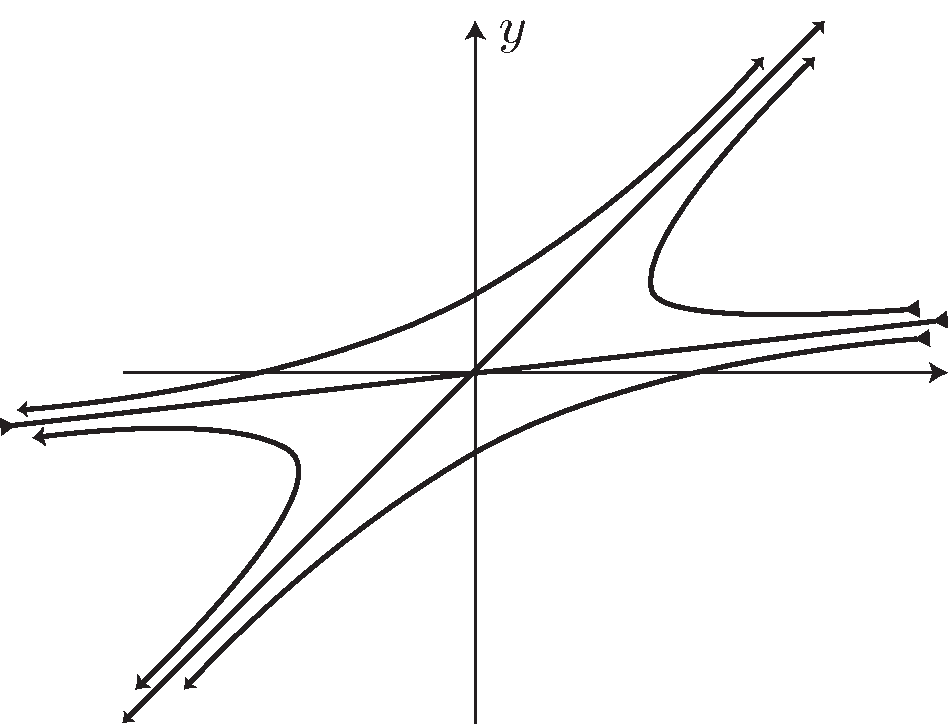
\includegraphics[width=4.5cm]{Graficos/figura5}
		\caption{Punto silla}
		\label{fig:M-5}
	\end{figure}

El origen es un punto silla si el retrato de fase muestra que a este punto tienden y hacia él entran dos semirectas con extremos en el origen cuando \(t\to\infty\) y hay otras dos semirectas que salen del origen cuando \(t\to-\infty\). Entre estas cuatro semirectas hay cuatro regiones, las cuales contienen una familia de trayectorias en forma de hipérbolas; estas trayectorias no tienden hacia el origen cuando , sino que son asintóticas a alguna de las semirectas. 

%
\vspace{0.75\baselineskip}
	\textbf{Centros (o vórtices)}\newline

\vspace{-1\baselineskip}
	\begin{figure}[H]
		\captionsetup{justification=centering, labelfont=footnotesize, font=footnotesize}
		\centering
		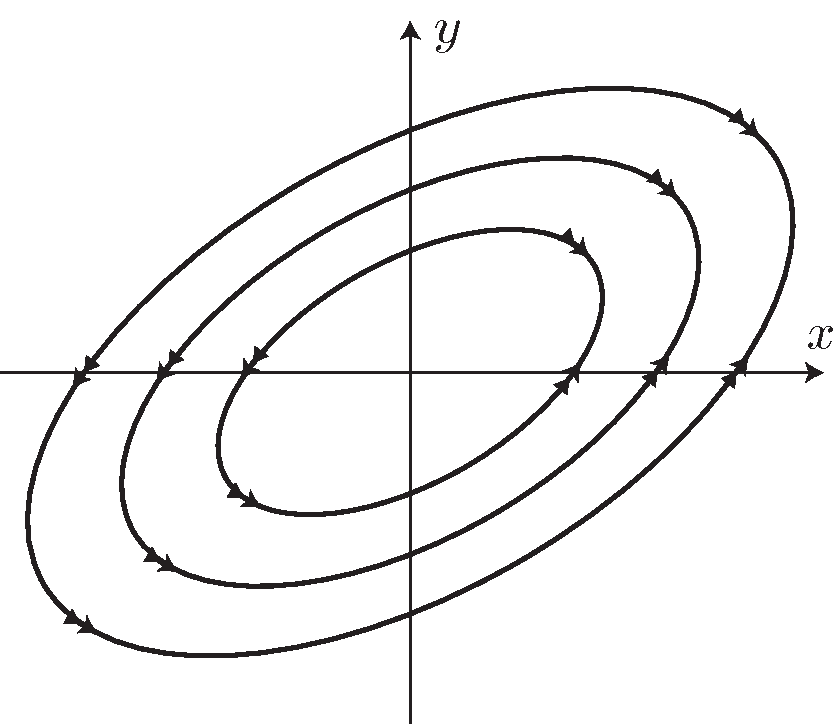
\includegraphics[width=4.5cm]{Graficos/figura6}
		\caption{Centro (estable)}
		\label{fig:M-6}
	\end{figure}

Es un punto crítico que está rodeado por una familia de trayectorias cerradas. Ninguna trayectoria tiende a él cuando \(t\to\pm\infty\).

\begin{ejem}
		Sea el sistema \(\nicefrac{dx}{dt}=-y\), \(\nicefrac{dy}{dt}=x\), el origen  es el único punto crítico.  Su solución general es:
		\[
		x(t) = -c_1 \sen t + c_2 \cos t 
		\yds
		y(t) = c_1 \sen t + c_2 \cos t.
		\]
		La solución que satisface las condiciones iniciales \(x(0)=1\), \(y(0)=0\) es  \(x=\cos t\), \(y=\sin t\), y la solución que satisface \(x(0)=0\), \(y(0)=1\) es \(x=-\sen t=\cos(t+\nicefrac{\pi}{2})\), \(y=\sen(t+\nicefrac{\pi}{2})\). Estas dos soluciones definen la misma trayectoria \(\Gamma\) que es la circunferencia \(x^2+y^2=1\) recorrida en sentido positivo (antihorario). En este caso \((0,0)\) es un centro.
		
		\vspace{-1\baselineskip}
	\begin{figure}[H]
		\captionsetup{justification=centering, labelfont=footnotesize, font=footnotesize}
		\centering
		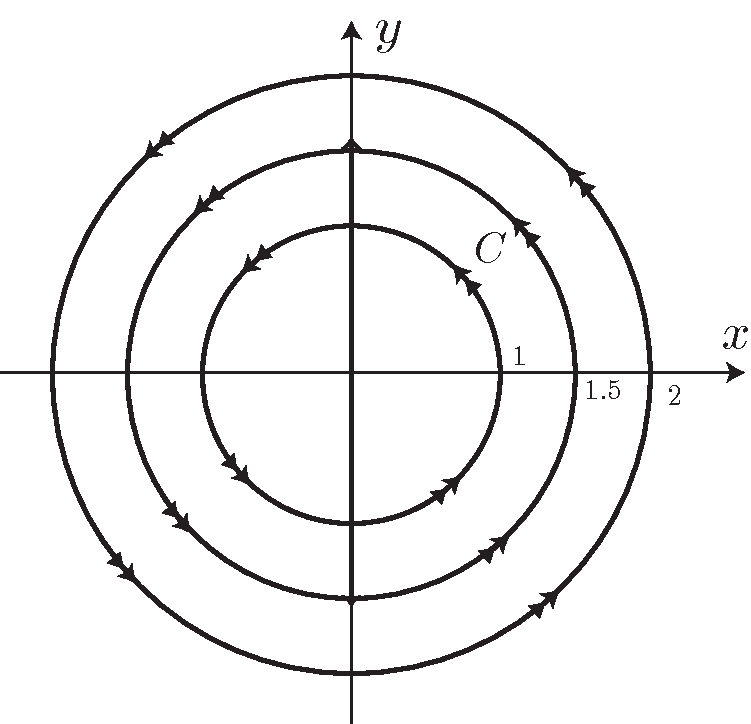
\includegraphics[width=4.5cm]{Graficos/figura7}
		\caption{Centro (estable)}
		\label{fig:M-7}
	\end{figure}		
	%
	\end{ejem}	

\newpage
%
%\vspace{0.75\baselineskip}
	\textbf{Focos}\newline

Un punto crítico se llama foco o punto espiral si el retrato de fase muestra que hacia él tienden (o salen de él) las trayectorias de una familia que gira en forma de espiral un número infinito de veces cuando \(t\to\pm\infty\).	Nótese que aunque las trayectorias tienden al origen, no entran a él en una dirección determinada, es decir, \(\displaystyle\lim_{t\to\infty}\nicefrac{dy}{dx}\) no existe.

\vspace{-1\baselineskip}
	\begin{figure}[H]
		\captionsetup{justification=centering, labelfont=footnotesize, font=footnotesize}
		\centering
		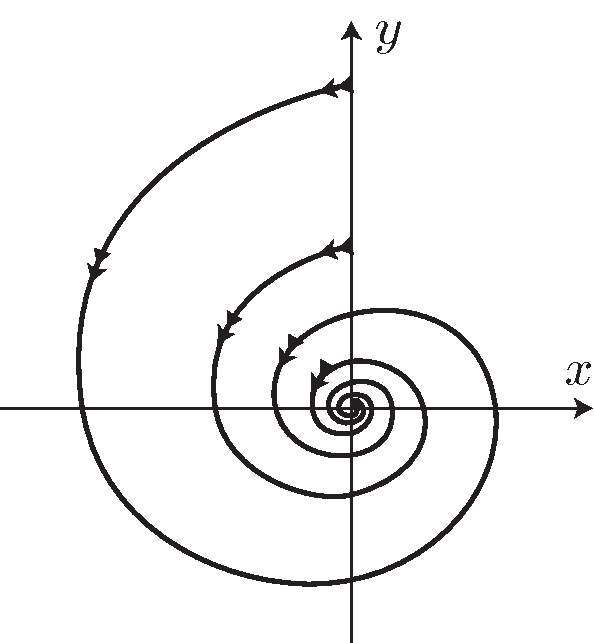
\includegraphics[width=4.5cm]{Graficos/figura8}
		\caption{Foco o espiral (asintóticamente estable)}
		\label{fig:M-8}
	\end{figure}

\begin{ejem}
	Sea \(a\) una constante arbitraria y considérese el sistema
	\[
	\begin{cases}
		\dfrac{dx}{dt}=ax - y,\vspace{0.3em}
		\\
		\dfrac{dy}{dt}=x+ay,
	\end{cases}
	\]

	Entonces \((0,0)\)es el único punto crítico, la ecuación diferencial de las trayectorias es:
			\[
			\dfrac{dx}{dy}=\dfrac{x+ay}{ax-y}.
			\]
			La cual en coordenadas polares queda: \(\nicefrac{dr}{d\theta}=ar\Longrightarrow r=ce^{a\theta}\) es la ecuación polar de las trayectorias.
			
			La dirección del recorrido se puede deducir del hecho que \(\nicefrac{dx}{dt}=-y\) cuando \(x=0\).
			
			Si \(a=0\)entonces el sistema se colapsa en \(\nicefrac{dx}{dt}=-y\), \(\nicefrac{dy}{dt}=x\) y se convierte en \(r=c\), que es la ecuación polar de la familia de circunferencias \(x^2+y^2=c^2\), en este caso se dice que cuando el parámetro \(a=0\)se ha producido una bifurcación, a este punto se lo llama de bifurcación, en esencia es un punto de donde las soluciones cambian cualitativamente de estable (o asintóticamente estables) a inestables o viceversa (ver figura \ref{fig:M-9}).
	
	\vspace{-1\baselineskip}
	\begin{figure}[H]
		\captionsetup{justification=centering, labelfont=footnotesize, font=footnotesize}
		\centering
		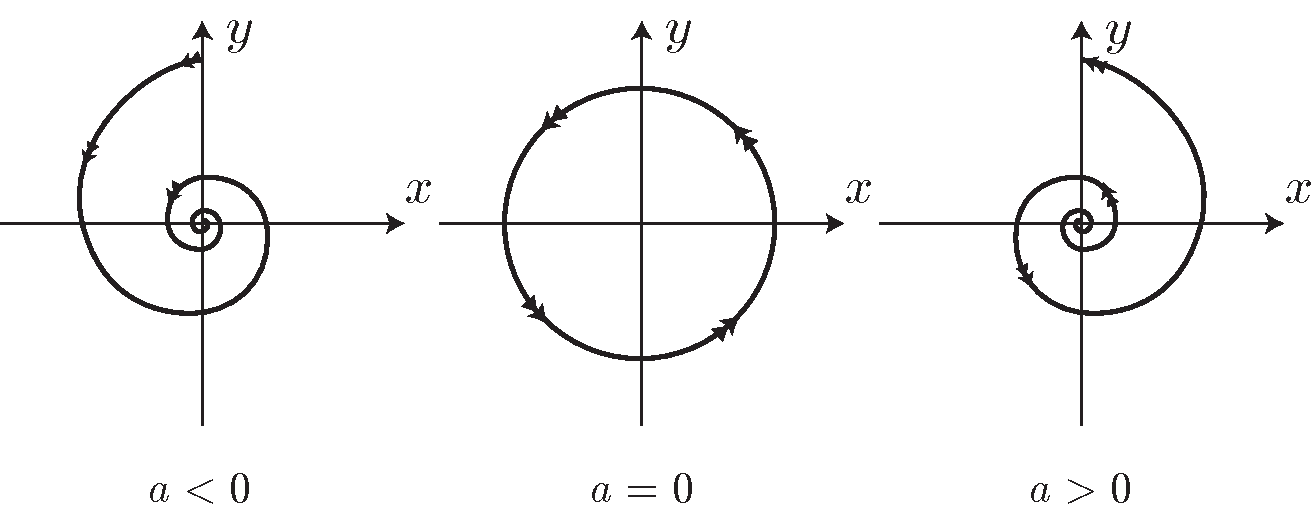
\includegraphics[scale=0.4]{Graficos/figura9}
	
		\footnotesize		
		\hspace{-2.5em}
		(a) Asin. estable	\qquad\quad
		(b) Estable		\qquad\quad
		(c) Inestable
		\caption{Bifurcación}
		\label{fig:M-9}
	\end{figure}
	
\end{ejem}


\neodefi{Estabilidad}

\begin{definicion}
				Si \((0,0)\) es un punto crítico de \eqref{m-1}, se dice que es \emph{\textbf{estable}} si para cada \(R>0\) existe un \(r>0\), con \(r\leq R\), tal que toda trayectoria que está dentro del círculo \(x^2+y^2=r^2\), para algún  \(t=t_0\), permanece en el círculo \(x^2+y^2=R^2\) para todo \(t>t_0\), es decir, si todas las trayectorias que están suficientemente cerca al punto crítico permanecen cercanas a él (ver figura \ref{fig:M-10}).

\vspace{-1\baselineskip}
	\begin{figure}[H]
		\captionsetup{justification=centering, labelfont=footnotesize, font=footnotesize}
		\centering
		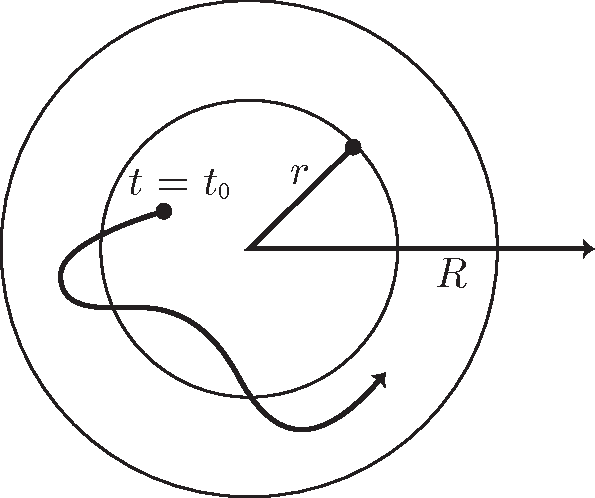
\includegraphics[width=4.5cm]{Graficos/figura10}
	
		\caption{}
		\label{fig:M-10}
	\end{figure}
\end{definicion}

\neodefi{Asintóticamente estable}

\begin{definicion}
	Si el punto crítico es estable y existe un círculo \(x^2+y^2=r_0^2\), tal que toda trayectoria que está dentro de él para algún \(t=t_0\), tiende al origen cuando \(t\to\infty\).
\end{definicion}


\begin{definicion}
	Si el punto crítico no es estable, se dice que es inestable.
\end{definicion}






\newpage

%
%
%
\subsubsection{Puntos críticos y estabilidad para sistemas lineales}
%
%
%

Se considera el sistema
\begin{equation}\label{m-6}
	\begin{cases}
		\dfrac{dx}{dt}=a_1 x + b_1 y,\vspace{0.3em}
		\\
		\dfrac{dy}{dt}=a_2 x + b_2 y,
	\end{cases}
\end{equation}
el cual tiene  a \((0,0)\) como punto crítico. Se supondrá que:
\begin{equation}\label{m-7}
	\begin{vmatrix}
		a_1	&	b_1	\\
		a_2	&	b_2
	\end{vmatrix}
	=	a_1b_2-a_2b_1\neq 0.
\end{equation}
Por tanto \((0,0)\) es el único punto crítico.

El sistema tiene una solución no trivial de la forma:
\vspace{0.5\baselineskip}
\begin{APAenumerate}
	\item \( \begin{aligned}[t]
	X_1 = \binom{x}{y}
		= e^{m_1 t } \binom{A_1}{B_1}
	;
	\qquad
	X_2 = \binom{x}{y}
		= e^{m_2 t } \binom{A_2}{B_2},
	\end{aligned}
	\)
	donde \(m_{1,2}\) son raíces distintas de la ecuación cuadrática: 
	\begin{equation}\label{m-8}
		m^2-(a_1+b_1)m+(a_1b_2-a_2b_1)=0.
	\end{equation}
	Que se conoce como ecuación característica del sistema, y \(\binom{A_1}{B_1}\), \(\binom{A_2}{B_2}\) son los vectores propios asociados a los valores propios \(m_{1,2}\). La condición \eqref{m-7} implica que \(m\neq 0\).
	
	\vspace{1\baselineskip}
	\item O de la forma:
	\( \begin{aligned}[t]
	X_1 = \binom{x}{y}
		= e^{m t } \binom{A}{B}
	;
	\qquad
	X_2 = \binom{x}{y}
		= e^{m t } \left[ \binom{A_1}{B_1} + t \binom{A}{B} \right]
	\end{aligned},
	\)
	donde \(\binom{A}{B}\) es el vector propio asociado al valor propio \(m\) de multiplicidad 2, y  \(\binom{A_1}{B_1}\) es el vector propio generalizado de rango 2 de \(m\).
\end{APAenumerate}

%
\neodefi{Caracterización de la naturaleza del punto crítico}

\begin{teorema}\label{teo-1}
	Sean \(m_1\) y \(m_2\) las raíces del polinomio característico. La naturaleza del punto crítico esta determinada por estas raíces.
\end{teorema}

Casos principales:
\begin{itemize}[leftmargin=15pt]
	\item[A:] Si las raíces \(m_1\) y \(m_2\) son reales, distintas y del mismo signo, entonces es un nodo.
	\item[B:] Si las raíces \(m_1\) y \(m_2\) son reales, distintas y de signos opuestos, entonces es un punto de silla.
	\item[C:] Si las raíces \(m_1\) y \(m_2\) son complejas conjugadas pero no imaginarias puras, entonces es un foco.
	\item[D:] Si las raíces \(m_1\) y \(m_2\) son reales e iguales, entonces es un nodo.
	\item[E:] Si las raíces \(m_1\) y \(m_2\) son imaginarias puras, entonces es un centro.
\end{itemize}

\newpage

\begin{observ}
	Para el Caso A, se puede tener:
	
	Si \(m_1<m_2<0\) se tiene un nodo impropio (asintóticamente estable)
	\vspace{-1\baselineskip}
	\begin{figure}[H]
		\captionsetup{justification=centering, labelfont=footnotesize, font=footnotesize}
		\centering
		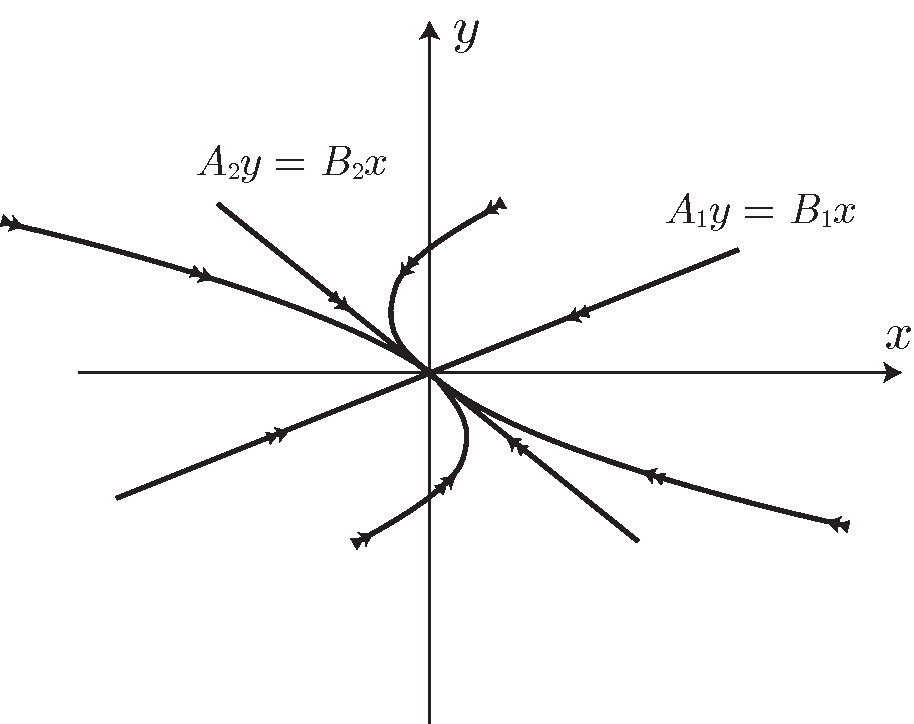
\includegraphics[width=4.5cm]{Graficos/figura11}
	
		\caption{Nodo impropio (asintóticamente estable)}
		\label{fig:M-11}
	\end{figure}
	
	Si \(m_1>m_2>0\) se tiene un nodo impropio (asintóticamente inestable)
	\vspace{-1\baselineskip}
	\begin{figure}[H]
		\captionsetup{justification=centering, labelfont=footnotesize, font=footnotesize}
		\centering
		\includegraphics[width=4.5cm]{Graficos/figura12}
	
		\caption{Punto silla (inestable)}
		\label{fig:M-12}
	\end{figure}
	
	Para el Caso B, se tiene un punto de silla
	\vspace{-1\baselineskip}
	\begin{figure}[H]
		\captionsetup{justification=centering, labelfont=footnotesize, font=footnotesize}
		\centering
		\includegraphics[width=4.5cm]{Graficos/figura13}
	
		\caption{Focos (asintóticamente estables)}
		\label{fig:M-13}
	\end{figure}
	
	Para el Caso D, se tiene  dos casos:
	\begin{APAenumerate}
		\item \(a_1=b_2\neq 0\), \(a_2=b_1=0\) se tiene un nodo propio o nodo estrella asintóticamente estable
		\vspace{-1\baselineskip}
	\begin{figure}[H]
		\captionsetup{justification=centering, labelfont=footnotesize, font=footnotesize}
		\centering
		\includegraphics[width=4.5cm]{Graficos/figura14}
	
		\caption{Nodo propio o nodo estrella (asintóticamente estable)}
		\label{fig:M-14}
	\end{figure}
		
		
		\item Todas las demás posibilidades dan como resultado un nodo impropio asintóticamente estable
		\vspace{-1\baselineskip}
	\begin{figure}[H]
		\captionsetup{justification=centering, labelfont=footnotesize, font=footnotesize}
		\centering
		\includegraphics[width=4.5cm]{Graficos/figura15}
	
		\caption{Nodo impropio (asintóticamente estable)}
		\label{fig:M-15}
	\end{figure}
	\end{APAenumerate}

Para el Caso E, el punto \((0,0)\) es un centro estable
\vspace{-1\baselineskip}
	\begin{figure}[H]
		\captionsetup{justification=centering, labelfont=footnotesize, font=footnotesize}
		\centering
		\includegraphics[width=4.5cm]{Graficos/figura6}
	
		\caption{Centro (estable)}
		\label{fig:M-16}
	\end{figure}
\end{observ}


%
\neodefi{Criterio de estabilidad}


\begin{teorema}\label{teo-2}
	El punto crítico \((0,0)\) del sistema es estable si y solo si  ambas raíces de la ecuación auxiliar: \(m^2-(a_1+b_2)m+(a_1b_2-a_2b_a)=0\) tienen partes reales no positivas, y es  asintóticamente estable si y solo si 	ambas raíces tienen partes reales negativas.
\end{teorema}

En efecto: si la ecuación auxiliar se escribe de la forma:
\[
(m-m_1)(m-m_2)=m^2-(m_1+m_2)m+m_1m_2=m^2+pm+1=0,
\]
entonces los cinco casos anteriores se pueden escribir en términos de \(p\) y \(q\) y para ello se utiliza el plano \(pq\).

El eje \(p\) está excluido ya que \(q=m_1m_2=a_1b_2-a_2b_1\neq 0\). Por tanto toda la información se puede extraer de \(m_{1,2}=\nicefrac{\big(-p\pm\sqrt{p^2-4q}\big)}{2}\).
\vspace{-1\baselineskip}
	\begin{figure}[H]
		\captionsetup{justification=centering, labelfont=footnotesize, font=footnotesize}
		\centering
		\includegraphics[scale=0.35]{Graficos/figura17}
	
		\caption{ }
		\label{fig:M-17}
	\end{figure}

De la figura \ref{fig:M-17} se tiene que:
\begin{APAitemize}
	\item Por encima de la parábola \(p^2-4q=0\) se tiene que \(p^2-4q<0\). Luego \(m_{1,2}\) son números 	complejos y estos son imaginarios puros si y solo si \(p=0\); estos son los caso C y E de focos y centros.
	\item Por debajo del eje \(p\) se tiene \(q<0\) lo que implica que las raíces son reales distintas y de signos opuestos, por tanto es un punto silla o sea el caso B.
	\item La zona entre la parábola y el eje \(p\) (excluido este eje e incluyendo a la parábola), se caracteriza porque \(p^2-4q\geq 0\), \(q>0\),  de donde las raíces son reales y del mismo signo y sobre la parábola	son iguales, por tanto son nodos y son los casos A y D.
	\item El primer cuadrante excluyendo a los ejes, es una región con estabilidad asintótica; el eje positivo \(q\) corresponde a centros y por tanto es estable; el segundo, tercero y cuarto cuadrante son regiones inestables.
\end{APAitemize}


%
\neodefi{Criterio de estabilidad asintótica}

\begin{teorema}
	El punto critico \((0,0)\) es asintóticamente estable si y solo si  los coeficientes \(p=-(a_1+b_2)\), \(q=a_1b_2-a_2b_1\) de la ecuación auxiliar son ambos positivos.
\end{teorema}

%\newpage

%
%
%
\subsubsection{Criterio de estabilidad por el método de Liapunov}
%
%
%
Considerando el sistema autónomo
\begin{equation}\label{m-9}
	\begin{cases}
		\dfrac{dx}{dt}=F(x,y) ,\vspace{0.3em}
		\\
		\dfrac{dy}{dt}=G(x,y),
	\end{cases}
\end{equation}

Suponiendo que tiene un punto crítico aislado; sea \((0,0)\) dicho punto (un punto crítico \(( x_0 , y_0 )\) se puede
llevar al origen por medio de una traslación). Sea \(\Gamma\big(x(t),y(t)\big)\) una trayectoria del sistema y sea \(E( x , y )\) una función continua con primeras derivadas parciales continuas en una región que contiene a la trayectoria. Si un punto \(( x, y )\) se mueve a lo largo de la trayectoria de acuerdo a las ecuaciones: \(x = x ( t )\), \(y = y ( t )\), entonces: 
\[
	E(x,y)=E\big(x(t),y(t)\big)=E(t).
\]
Es una función de \(t\) sobre \(\Gamma\), su razón de cambio es:
\begin{equation}\label{m-10}
	E'(x,y)=\dfrac{dE}{dt}=\dfrac{\partial E}{\partial x}\dfrac{dx}{dt}+\dfrac{\partial E}{\partial y}\dfrac{dy}{dt}=\dfrac{\partial E}{dx}F+\dfrac{\partial E}{\partial y}G.
\end{equation}
Esta fórmula es la idea principal de Liapunov.

\begin{definicion}
	Suponiendo que E \(( x , y )\) es continua y tiene primeras derivadas parciales continuas en una región que contiene al origen. Si \(E ( 0 , 0 ) = 0\) y
	\begin{APAenumerate}
		\item si \(E(x,y)>0\) y \((x,y)\neq(0,0)\), se dice que \(E(x,y)\) es definida positiva,
		\item si \(E(x,y)<0\) y \((x,y)\neq(0,0)\), se dice que \(E(x,y)\) es definida negativa,
		\item si \(E(x,y)\geq 0\) y \((x,y)\neq(0,0)\), se dice que \(E(x,y)\) es semidefinida positiva,
		\item si \(E(x,y)\leq 0\) y \((x,y)\neq(0,0)\), se dice que \(E(x,y)\) es semidefinida negativa.
	\end{APAenumerate}
\end{definicion}

\begin{observ}\quad
	\begin{APAitemize}
		\item \(E(x,y)=ax^{2m} + by^{2n}\) con \(a>0\), \(b>0\) y \(m\), \(n\) enteros positivos, es definida positiva.
		\item \(E(x,y)\) es definida negativa si y solo si \(-E(x,y)\) es definida positiva.
		\item Si \(E(x,y)\) es definida positiva, entonces \(z=E(x,y)\) es la ecuación de una superficie que podría parecerse a un paraboloide abierto hacia arriba y tangente al plano \(xy\) en el origen (ver figura \ref{fig:M-18}).
		%
		\vspace{-1\baselineskip}
	\begin{figure}[H]
		\captionsetup{justification=centering, labelfont=footnotesize, font=footnotesize}
		\centering
		\includegraphics[scale=0.35]{Graficos/figura18}
	
		\caption{ }
		\label{fig:M-18}
	\end{figure}	\end{APAitemize}
\end{observ}


\neodefi{Función de Liapunov}

\begin{definicion}
	Se dice que \(E(x,y)\) es una \emph{\textbf{función de Liapunov}} para el sistema autónomo, si:
	\begin{APAitemize}
		\item \(E(x,y)\) es continua, con primeras derivadas parciales continuas en una región que contiene al 	origen
		\item \(E(x,y)\) es definida positiva
		\item Existe la derivada de \(E\) a lo largo de trayectorias u órbitas del sistema y sea menor o igual que cero sobre la trayectoria, es decir, existe la derivada:
		\[
		\dfrac{\partial E}{\partial x}F+\dfrac{\partial E}{\partial y}G=E'\leq 0.
		\]
		\item Cuando \(\nicefrac{\partial E}{\partial x}F+\nicefrac{\partial E}{\partial y}G=E'<0\) se dice que \(E(x,y)\), se dice que es una \emph{\textbf{función de Liapunov}}	estricta.
	\end{APAitemize}
\end{definicion}


\neodefi{Criterio de Liapunov}

\begin{teorema}\quad
	\begin{APAenumerate}
		\item Si existe una función de Liapunov para el sistema, entonces el punto crítico \(( 0 , 0 )\) es estable.
		\item Si existe una función de Liapunov estricta para el sistema, entonces \((0,0)\) es un punto crítico asintóticamente estable.
		\item Si \(E'(x,y)\) es definida positiva, entonces el punto crítico \((0,0)\) es inestable.
	\end{APAenumerate}
\end{teorema}

\begin{ejem}
	La ecuación diferencial de una masa \(m\) sujeta a un resorte de constante \(k\) , en un medio que ofrece un amortiguamiento de coeficiente \(C\) es:
	\[
	m\dfrac{d^2x}{dt^2}+C\dfrac{dx}{dt}+kx=0.
	\]
	Analizar la estabilidad de su punto crítico.
\end{ejem}
\begin{proof}[Solución]
		El sistema autónomo equivalente es:
		\[
		\begin{cases}
		\dfrac{dx}{dt}=y,\vspace{0.3em}
		\\
		\dfrac{dy}{dt}=-\dfrac{k}{m}x-\dfrac{C}{m}y.
	\end{cases}
		\]
		Su único punto crítico es \((0,0)\). La energía cinética es \(\nicefrac{1}{2}my^2\) y la energía potencial (o energía almacenada en el muelle) es \(\int_{0}^{x}kx\,dx=\nicefrac{1}{2}kx^2\), luego la energía total es: \(E(x,y)=\nicefrac{1}{2}my^2+\nicefrac{1}{2}kx^2\), la cual es definida positiva.
		
		Como \(\nicefrac{\partial E}{\partial x}F+\nicefrac{\partial E}{\partial y}G=kxy+my\left(-\nicefrac{k}{m}x-\nicefrac{C}{m}y\right)=-Cy^2\leq 0\). Se tiene que \(E(x,y)\) es una función de Liapunov para el sistema y por tanto \((0,0)\) es estable.
		
		Se sabe que si \(C>0\) el punto crítico \((0,0)\) es asintóticamente estable, pero la función de Liapunov no detecta este hecho.
\end{proof}

\begin{ejem}[Resorte no lineal]
	Este es un ejemplo de masa \(m=1\) sujeta a un resorte no lineal, en el cual la fuerza restauradora es una función de la distancia de la masa al origen, sea \(-f(x)\) una función no lineal que representa la fuerza restauradora tal que \(f(0)=0\) y \(xf(x)>0\), \(x\neq 0\); no hay fricción. La ecuación de su movimiento es: \(\nicefrac{d^2x}{dt^2}+f(x)=0\). Analizar la estabilidad de su punto crítico.
\end{ejem}
\begin{proof}[Solución]
		El sistema autónomo equivalente es: 
		\[
			x'=y \yds y'=-f(x).
		\]
		
		Su único punto crítico es \((0,0)\). La energía cinética es \(\nicefrac{1}{2}x'^2=\nicefrac{1}{2}y^2\) y la energía potencial es: 
		\[
		F(x)=\displaystyle\int_{0}^{x}f(x)\,dx.
		\]
		Y la energía total es:
		\[
		E(x,y)=F(x)+\dfrac{1}{2}y^2.
		\]
		Como \(x\) y \(f(x)\) tienen el mismo signo entonces \(F(x)\geq0\) y por tanto \(E(x,y)\) es definida positiva. Además,
		\[
		E'(x,y)=F'(x)x'+yy'=f(x)y+y\big(-f(x)\big)=0.
		\]
		Es decir, es semidefinida negativa y por el teorema el punto crítico \((0,0)\) es estable. Igual que sucede con un resorte lineal, se puede demostrar que este punto crítico es un centro.
\end{proof}


\begin{ejem}
	Analizar la estabilidad del sistema:
	\[
	\begin{cases}
		x'=-x-\dfrac{x^3}{3}-x\sen y,
		\\
		y'=-y-\dfrac{y^3}{3}.
	\end{cases}
	\]
\end{ejem}
	\begin{proof}[Solución]
		El origen \((0,0)\) es el único punto crítico. Sea \(E(x,y)=\nicefrac{1}{2}(x^2+y^2)\), luego
		\begin{align*}
			E'(x,y)&=x\left(-x-\dfrac{x^3}{3}-x\sen y\right)+y\left(-y-\dfrac{y^3}{3}\right)\\
				&=-x^2-\dfrac{x^4}{3}-y^2-\dfrac{y^4}{3}-x^2\sen y\\
				&\leq -\dfrac{x^4}{3}-y^2-\dfrac{y^4}{3}<0.
		\end{align*}
		Es decir, \(E'\) es definida negativa, por tanto \((0,0)\) es asintóticamente estable.
	\end{proof}


\begin{ejem}
	Analizar la estabilidad del punto crítico del sistema:
	\[
	\begin{cases}
		x'=-2xy
		\\
		y'=x^2-y^2
	\end{cases}
	\]
\end{ejem}
	\begin{proof}[Solución]
		El origen \((0,0)\) es un punto crítico asilado. Sea \(E(x,y)=ax^{2m}+by^{2m}\), luego:
		\begin{align*}
			E'(x,y)&=2amx^{2m-1}(-2xy)+2by^{2n-1}(x^2-y^2)\\
				&=\left(-4amx^{2n}y+2bnx^2y^{2n-1}\right)-2nby^{2n+2} .
		\end{align*}
		Si: \(m=1\), \(n=1\), \(a=1\), \(b=2\) el paréntesis se anula, y se tiene: \(E(x,y)=x^2+2y^2\) es definida positiva y \(\nicefrac{\partial E}{\partial x}F+\nicefrac{\partial E}{\partial y}G=-4y^2\) es semidefinida negativa, de donde: \((0,0)\) es estable.
	\end{proof}



\begin{teorema}
	La función \(f(x,y)=ax^2+bxy+cy^2\) es:
	\begin{APAitemize}
		\item definida positiva si y solo si  \(a>0\) y \(b^2-4ac<0\),
		\item semidefinida positiva si y solo si \(a>0\) y \(b^2-4ac\leq 0\),
		\item definida negativa si y solo si \(a<0\) y \(b^2-4ac<0\),
		\item semidefinida negativa si y solo si \(a<0\) y \(b^2-4ac\leq 0\).
	\end{APAitemize}
\end{teorema}



%
%
%
\subsubsection{Linealización de sistemas no lineales}
%
%
%
Considere el sistema autónomo
\begin{equation}\label{m-11}
	\begin{cases}
		x'=F(x,y) ,
		\\
		y'=G(x,y),
	\end{cases}
\end{equation}
con un punto crítico asilado en \((x_0,y_0)\) (es decir \(F(x_0,y_0)=G(x_0,y_0)=0\)). Si \(F(x,y)\) y \(G(X,y)\) se pueden desarrollar en series de potencias alrededor de \((x_0,y_0)\), entonces si: \(u=x-x_0\), \(v=y-y_0\), entonces:
\begin{align}
	u'=x'&=F(x_0+u,y_0+v)\nonumber\\
		&=F(x_0,y_0)+u\dfrac{\partial F}{\partial x}(x_0,y_0)+v\dfrac{\partial F}{\partial y}(x_0,y_0)+\mathcal{O}(u,v,uv)\nonumber\\
		&=u\dfrac{\partial F}{\partial x}+v\dfrac{\partial F}{\partial y}+\mathcal{O}(u,v,uv)\label{m-12}
\end{align}
Similar:
\begin{equation}\label{m-13}
	v'=y'=u\dfrac{\partial G}{\partial x}+v\dfrac{\partial G}{\partial y}+\mathcal{O}'(u,v,uv).
\end{equation}
En forma matricial, se tiene que:
\begin{equation}\label{m-14}
	\begin{pmatrix} u' \\ v' \end{pmatrix}
	= \begin{pmatrix} \dfrac{\partial F}{\partial x} & \dfrac{\partial F}{\partial y} \\
\dfrac{\partial G}{\partial x} & \dfrac{\partial G}{\partial y} \end{pmatrix} \begin{pmatrix} u \\ v\end{pmatrix}+\begin{pmatrix} \mathcal{O}(u,v,uv) \\ \mathcal{O}'(u,v,uv)\end{pmatrix}.
\end{equation}

La matriz
\[
	J(F,G)(x_0,y_0)=\begin{pmatrix} \dfrac{\partial F}{\partial x}(x_0,y_0) & \dfrac{\partial F}{\partial y}(x_0,y_0) \\[1em]
\dfrac{\partial G}{\partial x}(x_0,y_0) & \dfrac{\partial G}{\partial y}(x_0,y_0)\end{pmatrix}
\]
se llama la \emph{\textbf{matriz Jacobiana}} del sistema evaluada en el punto crítico \((x_0,y_0)\). Cuando \(|u|\), \(|v|\) son pequeños, es decir, cuando \((u,v)\to(0,0)\) los términos de segundo orden y de orden superior son pequeños. Despreciando estos términos, se conjetura que el comportamiento cualitativo de \eqref{m-14} es similar al del sistema lineal asociado:
\begin{equation}\label{m-15}
	\begin{pmatrix} u' \\ v' \end{pmatrix}=\begin{pmatrix} \dfrac{\partial F}{\partial x} & \dfrac{\partial F}{\partial y} \\ \dfrac{\partial G}{\partial x} & \dfrac{\partial G}{\partial y} \end{pmatrix}	\begin{pmatrix} u \\ v \end{pmatrix},
\end{equation}
donde:
\[
\det\begin{pmatrix} \dfrac{\partial F}{\partial x}(x_0,y_0) & \dfrac{\partial F}{\partial y}(x_0,y_0) \\[1em]
\dfrac{\partial G}{\partial x}(x_0,y_0) & \dfrac{\partial G}{\partial y}(x_0,y_0)\end{pmatrix}\neq 0.
\]
Nótese que si \((x_0,y_0)\) es un punto crítico del sistema  de coordenadas \(XY\) entonces \((0,0)\) es el punto crítico en el nuevo sistema de coordenadas \(UV\). El proceso anterior de sustituir el sistema original por el  sistema lineal, se llama \emph{\textbf{linealización}} en el punto \((x_0,y_0)\).

Si se denota \(a_1=\nicefrac{\partial F}{\partial x}(x_0,y_0)\), \(b_1=\nicefrac{\partial F}{\partial y}(x_0,y_0)\), \(a_2=\nicefrac{\partial G}{\partial x}(x_0,y_0)\), \(b_2=\nicefrac{\partial G}{\partial y}(x_0,y_0)\), \(F(x_0,y_0)=0\) y \(G(x_0,y_0)=0\). El sistema puede ponerse de la forma:
\begin{equation}\label{m-16}
	\begin{cases}
		\dfrac{dx}{dt}= a_1x+b_1 y+f(x,y),	\vspace{0.3em}
		\\[1em]
		\dfrac{dy}{dt}= a_2 x+b_2 y+g(x,y).
	\end{cases}
\end{equation}
Suponiendo que
\begin{equation}\label{m-17}
	\det\begin{pmatrix} a_1 & b_1 \\ a_2 & b_2 \end{pmatrix} \neq 0,
\end{equation}
de tal manera que el sistema lineal asociado tiene a \((0,0)\) como punto crítico asilado y suponiendo que \(f\) y \(g\) son funciones continuas con primeras derivadas parciales continuas para todo \((x,y)\) y que
\begin{align}\label{m-18}
	\lim_{(x,y)\to(0,0)}\dfrac{f(x,y)}{\sqrt{x^2+y^2}} &= 0,
	\\
	\lim_{(x,y)\to(0,0)}\dfrac{g(x,y)}{\sqrt{x^2+y^2}}&= 0.
\end{align}
Estas dos últimas condiciones implican (por la continuidad) que \(f(0,0)=0\) y \(g(0,0)=0\), es decir, \((0,0)\) es un punto crítico. Se puede demostrar que es aislado. Con las restricciones indicadas se le llama \emph{\textbf{punto crítico simple}} de \eqref{m-16}.

Cuando se cumplen las condiciones \eqref{m-17} y \eqref{m-18}, se dice que  el sistema \eqref{m-16} es casi lineal o cuasi-lineal.

\begin{ejem}
	Comprobar que se cumplen las condiciones anteriores para el sistema:
	\[
	\begin{cases}
		\dfrac{dx}{dt}= -2x+3y+xy,	\vspace{0.3em}
		\\
		\dfrac{dy}{dt}= -x+y-2xy^2.
	\end{cases}
	\]
\end{ejem}
\begin{proof}[Solución]
		\[
		\det\begin{pmatrix} a_1 & b_1 \\ a_2 & b_2 \end{pmatrix}=\det\begin{pmatrix} -2 & 3 \\ -1 & 1 \end{pmatrix}=1\neq 0.
		\]
		Al usar coordenadas polares:
		\[
			\dfrac{|f(x,y)|}{\sqrt{x^2+y^2}}=\dfrac{|r^2\sin\theta\cos\theta|}{r}\leq r
			\yds
			\dfrac{|g(x,y)|}{\sqrt{x^2+y^2}}=\dfrac{|2r^3\sin^2\theta\cos\theta|}{r}\leq 2r^2.
		\]
		Cuando \((x,y)\to (0,0)\) se tiene:
		\[
			\lim_{r\to 0}\dfrac{f(x,y)}{r} = 0 \yds
			\lim_{r\to 0}\dfrac{g(x,y)}{r}=0.
		\]
		Luego \((0,0)\) es un punto crítico simple del sistema.
\end{proof}

\newpage

\neodefi{Tipos de punto crítico para sistemas no lineales}

\begin{teorema}\label{teo-6}
	Sea \((0,0)\) un punto crítico simple del sistema no lineal \eqref{m-16} y considere el sistema lineal asociado:
	\[
		\begin{cases}
			\dfrac{dx}{dt}=a_1 x + b_1 y,	\vspace{0.3em}
			\\
			\dfrac{dy}{dt}= a_2 x + b_2 y.
		\end{cases}
	\]
	Si el punto crítico \((0,0)\) del sistema asociado pertenece a alguno de los tres casos principales del  teorema \eqref{teo-1}, entonces el punto crítico \((0,0)\) es del mismo tipo para el sistema no lineal.
\end{teorema}

\begin{ejem}
	En el ejemplo anterior, analizar el punto crítico.
\end{ejem}
\begin{proof}[Solución]
	El sistema lineal asociado es:
	\[
		\begin{cases}
			\dfrac{dx}{dt}=-2 x + 3 y,	\vspace{0.3em}
			\\
			\dfrac{dy}{dt}=  {-x} +  y.
		\end{cases}
	\]
	La ecuación característica es: \(m^2+m+1=0\), con raíces \(m_{1,2}=-\nicefrac{1}{2}\pm\nicefrac{\sqrt{3}}{2}i\).
	
	Como las raíces son complejas conjugadas y no imaginarias puras, corresponde al caso C, lo que indica que \((0,0)\) es un foco para el sistema lineal, por lo que es un foco también para el sistema no lineal.
\end{proof}

\begin{observ}
	Aunque el tipo de punto crítico \((0,0)\) es el mismo para el sistema lineal y para el sistema no lineal, la apariencia de las trayectorias puede bien ser diferente. La figura \ref{fig:M-19} muestra un punto de silla para un sistema no lineal, en el cual se nota cierta distorsión, pero los rasgos cualitativos de las dos configuraciones son los mismos.
	
	\vspace{-1\baselineskip}
	\begin{figure}[H]
		\captionsetup{justification=centering, labelfont=footnotesize, font=footnotesize}
		\centering
		\includegraphics[width=4.5cm]{Graficos/figura19}
	
		\caption{ }
		\label{fig:M-19}
	\end{figure}
\end{observ}

\begin{observ}
Para los casos frontera no mencionados en el teorema \eqref{teo-6}, se tiene:
\begin{APAitemize}
	\item Si el sistema lineal asociado tiene un nodo frontera en \((0,0)\) (caso D), el sistema lineal puede tener
	un nodo o un foco.
	\item Si el sistema lineal asociado tiene un centro en \((0,0)\) (caso E), el sistema no lineal puede tener un
	centro o un foco.
\end{APAitemize}	
\end{observ}

\begin{ejem}
	Sea el sistema
	\[
	\begin{cases}
		\dfrac{dx}{dt}=-y+ax (x^2+y^2)  ,	\vspace{0.3em}
		\\
		\dfrac{dy}{dt}=x+ay(x^2+y^2),
	\end{cases}
	\]
	donde \(a\) es un parámetro. Mostrar que la linealización predice un centro o un foco en el origen. Mostrar que 	realmente corresponde a un foco.
\end{ejem}	
	\begin{proof}[Solución]
		El sistema lineal asociado es:
		\[
		\begin{cases}
		\dfrac{dx}{dt}=-y  ,	\vspace{0.3em}
		\\
		\dfrac{dy}{dt}=x.
	\end{cases}
		\]
		Para este último, \((0,0)\) es un centro, pero para el sistema no lineal es un foco, para mostrar ello, cambiemos el sistema a coordenadas polares. Sea \(x=r\cos\theta\), \(y=r\sin\theta\), \(r^2=x^2+y^2\), luego: \(rr'=xx'+yy'\). De donde:
		\[
		rr'=x\big(-y-ax(x^2+y^2)\big)+y\big(x+ay(x^2+y^2)\big)=ar^4.
		\]
		Por tanto: \(r'=ar^3\).
		
		Como \(\theta=\tan^{-1}(\nicefrac{y}{x})\), se obtiene: \(\theta'=\dfrac{xy'-yx'}{r^2}=1\).
		
		Obteniéndose el sistema en coordenadas polares:
		\[
		\begin{cases}
		r' = a r^3  ,	\vspace{0.3em}
		\\
		\theta' = 1.
		\end{cases}
		\]
		La solución es: \(r=\nicefrac{1}{\sqrt{c-2at}}\), \(\theta=t+t_0\) que corresponde a una familia de espirales.
		
		Luego si \(a<0\) entonces \(\lim_{t\to\infty}r(t)=0\), o sea que el origen es asintóticamente estable (es un sumidero) y si  \(a>0\) entonces \(\lim_{t\to-\infty}r(t)=0\) o sea que el origen es inestable (es una fuente), si \(a=0\) entonces \(r(t)=r_0\) o sea que el origen es un centro (ver figura \ref{fig:M-20}). Obsérvese que \(a=0\) es un punto de bifurcación.	\qedhere
		%
		\vspace{-1\baselineskip}
	\begin{figure}[H]
		\captionsetup{justification=centering, labelfont=footnotesize, font=footnotesize}
		\centering
		\includegraphics[scale=0.35]{Graficos/figura20}
	
		\caption{ }
		\label{fig:M-20}
	\end{figure}
		%
	\end{proof}


%
\neodefi{Estabilidad para sistemas no lineales}

\begin{teorema}\label{teo-7}
	Sea \((0,0)\) un punto crítico simple del sistema no lineal \eqref{m-16} y considérese el sistema lineal
	asociado.
	\begin{APAenumerate}
		\item Si el punto crítico \((0,0)\) del sistema lineal es asintóticamente estable, entonces también es asintóticamente estable para el sistema no lineal.
		\item Si el punto crítico\((0,0)\) del sistema lineal asociado es inestable, entonces es inestable para el sistema lineal.
		\item Si el punto crítico \((0,0)\) del sistema lineal asociado es estable pero no asintóticamente estable, entonces para el sistema no lineal puede ser estable, asintóticamente estable o inestable.
	\end{APAenumerate}
\end{teorema}

\begin{observ}
	En el caso 2 del teorema anterior se puede debilitar la hipótesis con la condición
	\begin{equation}\label{m-19}
		\det\begin{pmatrix} a_1 & b_1 \\ a_2 & b_2\end{pmatrix}=0
	\end{equation}
	y dejar las otras condiciones
	\[begin{align*}]
	\lim_{(x,y)\to(0,0)}\dfrac{f(x,y)}{\sqrt{x^2+y^2}}=0 \yds
	\lim_{(x,y)\to(0,0)}\dfrac{g(x,y)}{\sqrt{x^2+y^2}}=0.
	\]
	El resultado también se produce, es decir, si el punto crítico \((0,0)\) del sistema lineal asociado es inestable, entonces también lo es para el sistema no lineal.
\end{observ}


\begin{ejem}
	Sea el sistema:
	\[
	\begin{cases}
		\dfrac{dx}{dt}=-2x+3y+xy ,	\vspace{0.3em}
		\\
		\dfrac{dy}{dt}=-x+y-2xy^2,
	\end{cases}
	\]
	del sistema se puede concluir que 
	\[
		\det\begin{pmatrix} a_1 & b_1 \\ a_2 & b_2 \end{pmatrix}=1\neq 0.
	\]
	Es claro que  \((0,0)\) es un punto crítico simple, en este caso:
	\begin{align*}
		p&=-(a_1+b_2)=-(-2+1)=1>0\\
		q&=a_1b_2-a_2b_1=1>0.
	\end{align*}
	Luego, el punto crítico \((0,0)\) es asintóticamente estable para el sistema lineal y para el sistema no lineal.
\end{ejem}

\begin{ejem}
	La ecuación del movimiento para las oscilaciones forzadas de un péndulo es:
	\[
	\dfrac{d^2x}{dt^2}+\dfrac{c}{m}\dfrac{dx}{dt}+\dfrac{g}{a}\sen x=0,\quad c>0.
	\]
	El sistema no lineal es:
	\[
	\begin{cases}
		\dfrac{dx}{dt}=y ,	\vspace{0.3em}
		\\
		\dfrac{dy}{dt}=-\dfrac{g}{a}\sen x-\dfrac{c}{m}y.
	\end{cases}
	\]
	El cual puede escribirse de la forma
	\[
	\begin{cases}
		\dfrac{dx}{dt}=y ,	\vspace{0.3em}
		\\
		\dfrac{dy}{dt}=-\dfrac{g}{a}x-\dfrac{c}{m}y+\dfrac{g}{a}(x-\sen x).
	\end{cases}
	\]
	Se puede mostrar fácilmente que:
	\[
	\lim_{(x,y)\to(0,0)}\dfrac{x-\sen x}{\sqrt{x^2+y^2}}=0.
	\]
	Como el punto crítico \((0,0)\) es aislado del sistema lineal asociado
	\[
	\begin{cases}
		\dfrac{dx}{dt}=y ,	\vspace{0.3em}
		\\
		\dfrac{dy}{dt}=-\dfrac{g}{a}x-\dfrac{c}{m}y.
	\end{cases}
	\]
	Entonces \((0,0)\) es un punto crítico simple del sistema no lineal, además:
	\begin{align*}
		p&=-(a_1+b_2)=-\left(0-\dfrac{c}{m}\right)=\dfrac{c}{m}>0\\
		q&=a_1b_2-a_2b_1=0\left(-\dfrac{c}{m}\right)-1\left(-\dfrac{g}{a}\right)=\dfrac{g}{a}>0.
	\end{align*}
	Entonces el origen es un punto crítico asintóticamente estable del sistema lineal y también del no lineal. Esto refleja el hecho físico que si un péndulo se perturba ligeramente el movimiento resultante se extinguirá con el tiempo.
\end{ejem}


\begin{ejem}
	Hallar los puntos críticos, determinar su naturaleza y su estabilidad, para el siguiente sistema:
	\[
	\begin{cases}
		\dfrac{dx}{dt}=-2xy=F(x,y) ,	\vspace{0.3em}
		\\
		\dfrac{dy}{dt}=-x+y+xy-y^3=G(x,y).
	\end{cases}
	\]
\end{ejem}
\begin{proof}[Solución]
	La matriz Jacobiana es
	\[
	\begin{pmatrix} \dfrac{\partial F}{\partial x} & \dfrac{\partial F}{\partial y} \\ \dfrac{\partial G}{\partial x} & \dfrac{\partial G}{\partial y} \end{pmatrix}=\begin{pmatrix} -2y & -2x \\ -1+y & 1+x-3y^2 \end{pmatrix}.
	\]
	Para hallar los puntos críticos resolvemos el sistema:
	\[
	F(x,y)=G(x,y)=0.
	\]
	Obteniéndose como puntos críticos a \((0,0)\), \((0,1)\), \((0,-1)\).
	
	\begin{APAitemize}
		\item Para el punto crítico \((0,0)\) se tiene que la matriz Jacobiana es : \(\begin{bmatrix} 0 & 0 \\ -1 & 1 \end{bmatrix}\) y su determinante es  cero.
		
		El sistema lineal asociado es:
		\[
		\begin{cases}
			x' = a_1 x + b_1 y = 0,
			\\
			y' = a_2x+b_2y=-x+y.
		\end{cases}
		\]
		Los valores propios son \(\lambda_1=0\), \(\lambda_2=1\), los vectores propios asociados son \(\begin{pmatrix} 1 \\ 1\end{pmatrix}\), \(\begin{pmatrix} 0 \\ 1 \end{pmatrix}\) y la solución general es \(\begin{pmatrix} x \\ y \end{pmatrix}=\begin{pmatrix} c_1 \\ c_1+c_2e^t \end{pmatrix}\) que es una familia de semirectas paralelas el eje \(Y\) que comienzan en cada punto de la recta \(y = x\) alejándose de ella, por tanto todos los puntos críticos \(( x, x )\) son inestables, en particular \(( 0 , 0 )\) y por la nota anterior, se concluye que el sistema no lineal es inestable en \(( 0 , 0 )\) (ver figura \ref{fig:M-21})
		%
		\vspace{-1\baselineskip}
	\begin{figure}[H]
		\captionsetup{justification=centering, labelfont=footnotesize, font=footnotesize}
		\centering
		\includegraphics[scale=0.35]{Graficos/figura21}
	
		\caption{ }
		\label{fig:M-21}
	\end{figure}
	
	\item Para el punto \((1,0)\) la matriz Jacobiana es: \(\Big(\begin{smallmatrix} -2 & 0 \\ 0 & -2 \end{smallmatrix} \Big)\) y su determinante es diferente de cero. 
		
		Haciendo \(u=x-x_0=x\), \(v=y-y_0=y-1\), el sistema lineal asociado es:
		\[
		 \begin{pmatrix}u'\\v'\end{pmatrix}=\begin{pmatrix} \dfrac{\partial F}{\partial x} & \dfrac{\partial F}{\partial y} \\ \dfrac{\partial G}{\partial x} & \dfrac{\partial G}{\partial y}\end{pmatrix}\begin{pmatrix} u \\ v\end{pmatrix}=\begin{pmatrix}-2 & 0 \\ 0 & -2 \end{pmatrix}\begin{pmatrix} u \\ v\end{pmatrix}.
		\]
		Los valores propios del sistema lineal asociado son: \(\lambda_{1,2}=-2<0\), por el teorema \eqref{teo-1}, caso D, el punto crítico es un nodo estrella y por el teorema \eqref{teo-2} es asintóticamente estable para el sistema lineal asociado, por la observación del teorema \eqref{teo-6}, referente a los casos frontera y por el teorema \eqref{teo-7} es un nodo o un foco asintóticamente estable.
		
		
	\item Para el punto \((0,-1)\) la matriz Jacobiana es: \(\Big(\begin{smallmatrix} 2 & 0 \\ -2 & -2\end{smallmatrix}\Big)\) y su determinante es diferente de cero. Haciendo \(u=x-x_0=x\),  \(v=y-y_0=y+1\), el sistema lineal asociado es
		\[
		\begin{pmatrix}u'\\v'\end{pmatrix}=\begin{pmatrix} \dfrac{\partial F}{\partial x} & \dfrac{\partial F}{\partial y} \\ \dfrac{\partial G}{\partial x} & \dfrac{\partial G}{\partial y}\end{pmatrix}\begin{pmatrix} u \\ v\end{pmatrix}=\begin{pmatrix} 2 & 0 \\ -2 & -2\end{pmatrix}\begin{pmatrix} u \\ v\end{pmatrix}.
		\]
		Los valores propios  del sistema lineal asociado son: \(\lambda_1=2\), \(\lambda_2=-2\), por el teorema \eqref{teo-1}, el caso B, punto crítico es un punto silla y por el teorema \eqref{teo-2} es inestable para el sistema lineal asociado; entonces para el sistema no lineal, por el teorema \eqref{teo-6} y por el teorema \eqref{teo-7},	\((0,-1)\) es un punto silla inestable.	\qedhere
	\end{APAitemize}
\end{proof}


\begin{ejem}[Dos especies en competencia]
	Supóngase que dos especies liebres y ovejas compiten por el mismo tipo de alimento (grama) y esta cantidad de alimento es limitada, ignorando otros factores como depredadores, factores climáticos, otras fuentes de alimento. Las ecuaciones que modelan este fenómeno son las ecuaciones de Lotka--Volterra
	\[
	\begin{cases}
		x'=x(3-x-2y)=F(x,y),
		\\
		y'=y(2-x-y)=G(x,y),
	\end{cases}
	\]
	donde \(x(t)\) es la población de liebres y \(y(t)\) es la población de ovejas. Hallar los puntos críticos, definir el tipo y estabilidad.
\end{ejem}
\begin{proof}[Solución]
		Los puntos críticos son: \(A(0,0)\), \(B(0,2)\), \(C(3,0)\), \(D(1,1)\).
		
		El Jacobiano es: 
		\[
		J = \begin{pmatrix}\dfrac{\partial F}{\partial x} & \dfrac{\partial F}{\partial y} \\ \dfrac{\partial G}{\partial x} & \dfrac{\partial G}{\partial y} \end{pmatrix}=\begin{pmatrix} 3-2x-y & -2y \\ -y &  2-x-2y\end{pmatrix}.
		\]
		
		\begin{APAenumerate}
			\item Para el punto \(A(0,0)\), \(J=\Big(\begin{smallmatrix}  3 & 0 \\ 0 & 2\end{smallmatrix}\Big) \) y sus valores propios son: \(\lambda_1=3\), \(\lambda_2=2\), luego, \((0,0)\) es un nodo inestable, es decir las trayectorias salen tangencialmente del origen paralelas al vector propio \(v=\begin{pmatrix} 0 \\ 1\end{pmatrix}\) asociado al valor propio \(\lambda_2=2\).
			
			\item Para el punto \(B(0,2)\), \(J=\Big(\begin{smallmatrix}  -1 & 0 \\ -2 & 2 \end{smallmatrix}\Big) \) y sus valores propios son: \(\lambda_1=-1\), \(\lambda_2=2\), luego, \((0,2)\) es un nodo asintóticamente estable, las trayectorias entran al punto crítico en la dirección del vector propio \(v=\begin{pmatrix} 1 \\ -2\end{pmatrix}\) asociado al valor propio \(\lambda_1=-1\).
			
			\item Para el punto \(C(3,0)\), \(J=\Big(\begin{smallmatrix}  -3 & -6 \\ 0 & -1 \end{smallmatrix}\Big) \) y sus valores propios son: \(\lambda_1=-3\), \(\lambda_2=-1\), luego, \((3,0)\) es un nodo asintóticamente estable, las trayectorias entran al punto crítico en la dirección del vector propio \(v=\begin{pmatrix} 3 \\ -1\end{pmatrix}\) asociado al valor propio \(\lambda_1=-1\).
			
			\item Para el punto \(D(1,1)\), \(J=\Big(\begin{smallmatrix} -1 & -2 \\ -1 & -1 \end{smallmatrix}\Big) \) y sus valores propios son: \(\lambda_{1,2}=-1\pm\sqrt{2}\), luego, \((1,1)\) es un punto de silla y como \(p=-(a_1+a_2)=2\) y \(\det A=\left|\begin{smallmatrix} -1 & -2 \\ -1 & -1 \end{smallmatrix}\right|=-1<0\), entonces se tiene que \((1,1)\) es inestable.
		\end{APAenumerate}
	
	
	El retrato de fase mostrado en la figura \ref{fig:M-22} tiene la siguiente interpretación biológica: una de las dos especies 	inevitablemente se extingue, por ejemplo, por debajo de la curva l las trayectorias tienden al punto crítico \(C(3,0)\) lo cual quiere decir que las ovejas se extinguen; cuando las trayectorias están encima de la curva \(l\) las trayectorias tienden al punto crítico \(B(0,2)\) lo cual quiere decir que se extinguen las liebres.
	
	
	\end{proof}
	\newpage
%
	
	\begin{figure}[H]
		\captionsetup{justification=centering, labelfont=footnotesize, font=footnotesize}
		\centering
		\includegraphics[width=4.5cm]{Graficos/figura22}
	
		\caption{ }
		\label{fig:M-22}
	\end{figure}


\begin{ejem}[Dos especies: un depredador y una presa]
	Sea \(x(t)\) el número de presas (por ejemplo liebres) y \(y(t)\) el número de depredadores (por ejemplo lobos). A principios del siglo XX el matemático italiano Vito Volterra modeló este problema, haciendo las siguientes caracterizaciones:
	\begin{APAitemize}
		\item En ausencia de depredadores, la población de presas crece a la tasa natural \(\nicefrac{dx}{dt}=ax\), \(a>0\)
		\item En ausencia de presas, la población depredadora decrece a la tasa natural \(\nicefrac{dy}{dt}=-cy\), \(c>0\)
		\item Cuando las presas y los depredadores cohabitan el mismo lugar, las tasa naturales de crecimiento y   decrecimiento de presas y depredadores respectivamente son proporcionales al número de encuentros de ambos, es decir, son proporcionales a \(xy\). En consecuencia, el efecto de que los depredadores devoren a sus presas, produce una tasa decreciente de interacción \(-bxy\) con respecto a la población de presas \(x(t)\) y una tasa creciente \(dxy\) con respecto a la población de depredadores \(y(t)\).
		
		En consecuencia, sumando las tasan naturales y las tasa de interacción, se tienen las ecuaciones para una especie depredadora y una especie presa:
		\[
		\begin{cases}
		\dfrac{dx}{dt}=ax-bxy=x(a-by)  ,	\vspace{0.3em}
		\\
		\dfrac{dy}{dt}=-cy+dxy=y(-c+dx).
	\end{cases}
		\]
		Haciendo la consideración adicional de que en ausencia de depredadores el crecimiento de las presas es
		logístico, es decir, es directamente proporcional a su población como también a la diferencia con su población máxima y tomando \(a=b=c=d=1\), se tiene el sistema:
		\[
		\begin{cases}
		\dfrac{dx}{dt}=x-xy+\varepsilon x(1-x),	\vspace{0.3em}
		\\
		\dfrac{dy}{dt}=-y+xy.
	\end{cases}
		\]
	\end{APAitemize}
	Analizar la estabilidad, variando el parámetro \(\varepsilon\), para \(\varepsilon\geq 0\).
\end{ejem}
\begin{proof}[Solución]
		Los puntos críticos son \((0,0)\) y \((1,1)\). El Jacobiano es:
		\[
			J=\begin{pmatrix} \dfrac{\partial F}{\partial x} & \dfrac{\partial F}{\partial y} \\ \dfrac{\partial G}{\partial x} & \dfrac{\partial G}{\partial x}\end{pmatrix}=\begin{pmatrix} 1-y+\varepsilon(1-2x) & -x \\ y & -1+x\end{pmatrix}.
		\]
		Para \(\varepsilon=0\) tenemos (ver figura \ref{fig:M-23}):
		%
		\vspace{-1\baselineskip}
	\begin{figure}[H]
		\captionsetup{justification=centering, labelfont=footnotesize, font=footnotesize}
		\centering
		\includegraphics[width=4.5cm]{Graficos/figura23}
	
		\caption{Sistema depredador-presa, \(\varepsilon=0\)}
		\label{fig:M-23}
	\end{figure}
	
	\begin{APAenumerate}
			\item Para el punto crítico \((0,0)\), \(J= \Big(\begin{smallmatrix} 1 & 0 \\ 0 & -1\end{smallmatrix} \Big)\) y sus valores propios son: \(\lambda_1=1\), \(\lambda_2=1\), luego \((0,0)\) es un punto de silla estable.
			\item Para el punto crítico \((1,1)\), \(J= \Big(\begin{smallmatrix} 0 & -1 \\ 1 & 0 \end{smallmatrix}\Big) \) y sus valores propios son: \(\lambda_1=i\), \(\lambda_2=-i\), luego \((1,1)\) es un centro estable, las trayectorias giran alrededor el punto crítico.
		\end{APAenumerate}
	
	\vspace{1\baselineskip}
	Para \(0<\varepsilon<2\) tenemos (ver figura \ref{fig:M-24}):
	%
		%\vspace{-1\baselineskip}
	\begin{figure}[H]
		\captionsetup{justification=centering, labelfont=footnotesize, font=footnotesize}
		\centering
		\includegraphics[width=4.5cm]{Graficos/figura24}
	
		\caption{Sistema depredador-presa, \(\varepsilon \in (0,2)\)}
		\label{fig:M-24}
	\end{figure}

	\begin{APAenumerate}
		\item Para el punto crítico \((0,0)\), \(J= \Big(\begin{smallmatrix}  1+\varepsilon & 0 \\ 0 & -1 \end{smallmatrix} \Big) \) y sus valores propios son: \(\lambda_1=1+\varepsilon>0\), \(\lambda_2=-1\), luego \((0,0)\) es un punto de silla inestable.
		\item Para el punto crítico \((1,1)\), \(J= \Big(\begin{smallmatrix}  -\varepsilon & -1 \\ 1 & 0\end{smallmatrix} \Big) \) y sus valores propios son: \(\lambda_{1,2}=\dfrac{-\varepsilon\pm\sqrt{4-\varepsilon^2}i}{2}\), luego \((1,1)\) es un foco asintóticamente estable.
	\end{APAenumerate}

	\newpage
	Para \(\varepsilon=2\) tenemos (ver figura \ref{fig:M-25}):
	
	\begin{figure}[H]
		\captionsetup{justification=centering, labelfont=footnotesize, font=footnotesize}
		\centering
		\includegraphics[width=4.5cm]{Graficos/figura25}
	
		\caption{Sistema depredador-presa, \(\varepsilon=2\)}
		\label{fig:M-25}
	\end{figure}
	
	\begin{APAenumerate}
	\item Para el punto crítico \((0,0)\), \(J= \Big(\begin{smallmatrix}  3 & 0 \\ 0 & -1 \end{smallmatrix} \Big) \) y sus valores propios son: \(\lambda_1=-1\), \(\lambda_2=3\), luego \((0,0)\)  es un punto de silla inestable.
	\item Para el punto crítico \((1,1)\), \(J= \Big(\begin{smallmatrix}  -2 & -1 \\ 1 & 0 \end{smallmatrix} \Big) \) y sus valores propios son: \(\lambda_{1,2}=-1\), luego \((1,1)\) es un nodo o un foco asintóticamente estable.
\end{APAenumerate}


	Para \(\varepsilon>2\) tenemos (ver figura \ref{fig:M-26}):
	
	\begin{figure}[H]
		\captionsetup{justification=centering, labelfont=footnotesize, font=footnotesize}
		\centering
		\includegraphics[width=4.5cm]{Graficos/figura26}
	
		\caption{Sistema depredador-presa, \(\varepsilon>2\)}
		\label{fig:M-26}
	\end{figure}

	\begin{APAenumerate}
	\item Para el punto crítico \((0,0)\), \(J= \Big(\begin{smallmatrix}  1+\varepsilon & 0 \\ 0 & -1 \end{smallmatrix} \Big) \) y sus valores propios son: \(\lambda_1=\varepsilon+1\), \(\lambda_2=-1\), luego \((0,0)\) es un punto de silla inestable.
	\item Para el punto crítico \((1,1)\), \(J= \Big(\begin{smallmatrix}   -\varepsilon & -1 \\ 1 & 0 \end{smallmatrix} \Big) \) y sus valores propios son: \(\lambda_{1,2}=\dfrac{-\varepsilon\pm\sqrt{\varepsilon^2-4}}{2}<0\), luego \((1,1)\) es un nudo asintóticamente estable.
\end{APAenumerate}


Obsérvese que para soluciones para \(\varepsilon=0\) las soluciones son estructuralmente (son estables y periódicas) distintas de las \(\varepsilon>0\) (asintóticamente estables y no periódica, por este cambio estructural en las soluciones, se dice que en \(\varepsilon=0\) se produce una bifurcación.
\end{proof}









\nocite{bib-M}

}







\end{document}































